%Requires the memoir class 
\documentclass[twoside,11pt]{memoir}

%\usepackage{mathptmx}  % Times New Roman, but if you have Garamond 
                        % then use it;
                        % you are writing a book, not a newspaper column

\DoubleSpacing        % memoir's double spacing
\usepackage{rice}     % rice thesis package 


\usepackage{graphicx}
\usepackage{rotating}
\usepackage{caption}
\usepackage{subcaption}
\usepackage{multicol}

\usepackage{amsmath}
\usepackage{amssymb}
\usepackage{bm}
\usepackage{bbm}
%\usepackage{siunitx}
%\usepackage{txfonts}  % I used this one to summon the symbol for \lambdabar
\usepackage{lmodern}

\usepackage[numbers,compress]{natbib}

\usepackage[backref=page]{hyperref}
%\hypersetup{colorlinks=false}

\usepackage{parskip}
\usepackage{xfrac}
\usepackage{isomath}

\usepackage{memhfixc}

%%%%%%%%%%%%%%%%%%%%%%%%%%%%%%%%%%%%%%%%%%%%%%%%%%%%%%%%%%%%%%%%%%%
%%%% Definition of command shortcuts                           %%%%
%%%%%%%%%%%%%%%%%%%%%%%%%%%%%%%%%%%%%%%%%%%%%%%%%%%%%%%%%%%%%%%%%%%

\newcommand{\twos}[1]
     {\ensuremath{\hspace{-1pt}2\hspace{0.5pt}\hspace{0pt}S_{#1}\hspace{-1pt}}}
\newcommand{\twop}[1]
     {\ensuremath{\hspace{-1pt}2\hspace{0.5pt}\hspace{0pt}P_{#1}\hspace{-1pt}}}
\newcommand{\trep}[1]
     {\ensuremath{\hspace{-1pt}3\hspace{0.5pt}\hspace{0pt}P_{#1}\hspace{-1pt}}}

\newcommand{\cm}{\ensuremath{,\hspace{1pt}}}
\newcommand{\f}[1]{\ensuremath{F\hspace{-5pt}=\hspace{-4pt}#1}}
\newcommand{\mf}[1]{\ensuremath{m_{F}\hspace{-4pt}=\hspace{-4pt}#1}}
\newcommand{\mj}[1]{\ensuremath{m_{J}\hspace{-5pt}=\hspace{-4pt}#1}}
\newcommand{\mcm}{\ensuremath{\hspace{-4pt}}}

\newcommand{\red}
{\ensuremath{ \twos{1/2}\hspace{-0.0pt}\rightarrow\hspace{-0.0pt}\twop{3/2} }\ }
\newcommand{\uv}
{\ensuremath{ \twos{1/2}\hspace{-0.0pt}\rightarrow\hspace{-0.0pt}\trep{3/2} }\ }

\newcommand{\TD}{\ensuremath{ T_{D} }}
\newcommand{\TR}{\ensuremath{ T_{R} }}
\newcommand{\TF}{\ensuremath{ T_{F} }}

\newcommand{\one}{\ensuremath{|1\rangle }\ }
\newcommand{\two}{\ensuremath{|2\rangle }\ }

\newcommand{\isat}{ \ensuremath{ I_{\mathrm{sat}} } } 
\newcommand{\isatred}{ \ensuremath{ I_{sat\text{(red)}} } } 
\newcommand{\isatuv}{ \ensuremath{ I_{sat\text{(uv)}} } } 
\newcommand{\li} {\ensuremath{^{6}}Li\ }
\newcommand{\kb} { \ensuremath{k_{\mathrm{B}}}}

%%%%%%%%%%%%%%%%%%%%%%%%%%%%%%%%%%%%%%%%%%%%%%%%%%%%%%%%%%%%%%%%%%%

\newcommand{\bv}[1]{\ensuremath{\bm{#1}}}
\newcommand{\vo}{\ensuremath{V_{0}}}
\newcommand{\vvo}{\ensuremath{v_{0}}}
\newcommand{\bvo}{\ensuremath{\bv{V}_{0}}}
\newcommand{\er}{\ensuremath{E_{r}}}
\newcommand{\Lc}{\ensuremath{L_{\mathrm{c}}}}
\newcommand{\dsig}[1]{\ensuremath{ \frac{ d\,\sigma_{#1} }{d\,\Omega} }}
\newcommand{\dbl}{\ensuremath{ \uparrow\! \downarrow \, }}
\newcommand{\spup}{\ensuremath{ \uparrow }}
\newcommand{\spdn}{\ensuremath{ \downarrow}}


\newcommand{\ndbl} { \makebox[1em][c]{$\uparrow\! \downarrow \, $}}
\newcommand{\nvac} { \makebox[1em][c]{$0 $}}
\newcommand{\nspup}{ \makebox[1em][c]{$\uparrow$}}
\newcommand{\nspdn}{ \makebox[1em][c]{$\downarrow$}}
\newcommand{\nSspup}{ \makebox[0.7em][c]{$\uparrow$}}
\newcommand{\nSspdn}{ \makebox[0.7em][c]{$\downarrow$}}


\newcommand{\tbtwo}[4]{\scalebox{0.75}{\arraycolsep=1.0pt\def\arraystretch{0.7}$\left|\begin{array}{c|c}
\makebox[1em][c]{$#1$} &\makebox[1em][c]{$#2$} \\ \hline \makebox[1em][c]{$#3$}
&\makebox[1em][c]{$#4$} \\ \end{array}\right\rangle$ }}

%%%%%%%%%%%%%%%%%%%%%%%%%%%%%%%%%%%%%%%%%%%%%%%%%%%%%%%%%%%%%%%%%%%
% Compensated lattice
\newcommand{\rdiag}{\ensuremath{ r_{\text{\tiny{111}}} } }
\newcommand{\awaist}{\ensuremath{ \alpha_{w} }}  
\newcommand{\awaistevap}{\ensuremath{ \alpha_{w,\text{evap}} }}  
\newenvironment{myblock}{%
   \list{}{\rightmargin0pt}\item\relax
   % and maybe do more stuff
}{\endlist}


%%%%%%%%%%%%%%%%%%%%%%%%%%%%%%%%%%%%%%%%%%%%%%%%%%%%%%%%%%%%%%%%%%%
% Appendix on trap potentials 
\newcommand{\pin}{\ensuremath{ P_{\text{i}}} }
\newcommand{\pret}{\ensuremath{ P_{\text{r}}} }
\newcommand{\win}{\ensuremath{ w_{\text{in}}} }
\newcommand{\wret}{\ensuremath{ w_{\text{r}}} }
\newcommand{\wir}{\ensuremath{ w_{\text{ir}}} }

\newcommand{\pgr}{\ensuremath{ P_{\text{gr}}} }
\newcommand{\wgr}{\ensuremath{ w_{\text{gr}}} }

%%%%%%%%%%%%%%%%%%%%%%%%%%%%%%%%%%%%%%%%%%%%%%%%%%%%%%%%%%%%%%%%%%%
% Phase-contrast
\newcommand{\ts}[1]{\ensuremath{\tensorsym{#1}}}

\newcommand{\efield}{\ensuremath{\bv{\mathcal{E}}}}
\newcommand{\efieldo}{\ensuremath{\mathcal{E}_{0}}}
\newcommand{\epspol}{\ensuremath{\hat{\bv{\varepsilon}}}}
\newcommand{\dpol}{\ensuremath{\bv{\mathrm{P}}}}
\newcommand{\phcChi}{\ensuremath{\zeta}}

%%%%%%%%%%%%%%%%%%%%%%%%%%%%%%%%%%%%%%%%%%%%%%%%%%%%%%%%%%%%%%%%%%%
% Fermi Thermometry
\newcommand{\rf}[1]{\ensuremath{ R_{\mathrm{F}_{#1} } }}
\newcommand{\ldb}{\ensuremath{ \lambda_{\mathrm{th}} }}
\newcommand{\pli}{\ensuremath{ \mathrm{Li} }}

%%%%%%%%%%%%%%%%%%%%%%%%%%%%%%%%%%%%%%%%%%%%%%%%%%%%%%%%%%%%%%%%%%%
% Bragg
\newcommand{\sumOff}{\ensuremath{\sum_{\genfrac{}{}{-2pt}{}{m,n}{m\neq n}}}}
\newcommand{\sumOffn}{\ensuremath{\sum_{\genfrac{}{}{-2pt}{}{n}{n\neq m}}}}
\newcommand{\sumOffm}{\ensuremath{\sum_{\genfrac{}{}{-2pt}{}{m}{m\neq n}}}}
\newcommand{\sumOffij}{\ensuremath{\sum_{\genfrac{}{}{-2pt}{}{i,j}{i\neq j}}}}
\newcommand{\scrys}{\ensuremath{S_{\bv{Q}}^{\mathrm{crystal}}}}
\newcommand{\sq}{\ensuremath{S_{\bv{Q}}}}
\newcommand{\sPi}{\ensuremath{S_{\bv{\pi}}}}
\newcommand{\zoz}{\ensuremath{(0\hspace{0.3em}1\hspace{0.3em}0)}}
\newcommand{\ijk}{\ensuremath{(i\hspace{0.3em}j\hspace{0.3em}k)}}
%\newcommand{\zoz}{\ensuremath{(0\hspace{0.3em}\protect\raisebox{0.12em}{\protect\scalebox{0.75}[0.75]{-}}\hspace{-0.02em}1\hspace{0.3em}0)}}
\newcommand{\hhh}{\ensuremath{(\protect\raisebox{0.26em}{\protect\scalebox{0.75}[0.75]{-}}\sfrac{1}{2}\ \protect\raisebox{0.26em}{\protect\scalebox{0.75}[0.75]{-}}\sfrac{1}{2}\ \protect\raisebox{0.29em}{\protect\scalebox{0.5}[0.5]{+}}\sfrac{1}{2})}}


%%%%%%%%%%%%%%%%%%%%%%%%%%%%%%%%%%%%%%%%%%%%%%%%%%%%%%%%%%%%%%%%%%%
% Bragg paper
\newcommand{\half}{\frac{1}{2}}
\newcommand{\expect}[1]{\ensuremath{\langle{#1}\rangle}}
\newcommand{\ket}[1]{\ensuremath{|{#1}\rangle}}
\newcommand{\mathbfsf}[1]{\ensuremath{\bm{#1}}}
\newcommand{\debyew}{\ensuremath{e^{-2W_{\bv{Q}}(\tau)}}}

%%%%%%%%%%%%%%%%%%%%%%%%%%%%%%%%%%%%%%%%%%%%%%%%%%%%%%%%%%%%%%%%%%%
%\includeonly{
%part07,
%part08,
%part09,
%partB,
%partC,
%}

\DoubleSpacing

\begin{document}

\maxtocdepth{subsection}   % put everything into the ToC
\pagestyle{plain}          % pagestyle for the prelims

\frontmatter
\thetitlepage

%%%%%%%%%%%%%%%%%%%%%%%%%%%%%%%%%%%%%%%%%%%%%%%%%%%%%%%%%%%%%%%%%%%

% put your abstract here

\riceabstract
\pagestyle{empty}  % Rice requires no page numbering in the abstract


The Hubbard model contains only the essential ingredients to describe the
behavior of strongly interacting electrons moving in a periodic lattice.   It
describes particles that can tunnel between sites in the lattice and that
acquire an on-site interaction energy when two of them occupy the same lattice
site.   This simple model is a prominent example of how strongly correlated
phases emerge from simple Hamiltonians.  It gives rise to a Mott-metal
insulator transition,  and at a density of one particle per site shows an
antiferromagnetic ground state.  It is also considered to contain the essence
of high-temperature superconductivity as observed in the cuprates, a question
that remains open due to the difficulty in numerically accessing the solutions
of the model at densities different from one particle per site.  

In this work we have realized the Hubbard model with a spin mixture of
ultracold atoms in a simple cubic optical lattice.  Atoms in lattices have
emerged in the last decade as promising systems in which to perform quantum
simulations of condensed matter Hamiltonians.   In the laboratory we can create
defect-free optical lattice potentials with laser light, and we can control the
interactions between the atoms using a magnetic Feshbach resonance.  

For this work we implemented a novel compensated optical lattice setup, which
allows us to control the density of the sample and mitigate the
non-adiabaticity in the lattice loading process which often leads to heating of
the sample or to out of equilibrium distributions.   Using the compensated
optical lattice we are able to get closer to the ground state of the Hubbard
model than anybody before us has been able to do with ultracold atoms.

To demonstrate this achievement we use spin-sensitive Bragg scattering of light
to measure the spin-structure factor, a measure of the antiferromagnetic
correlations in the collection of spins.  Measurements of the spin-structure
factor are compared to results of theoretical calculations to establish precise
thermometry for the atoms in the lattice.  We have also studied the
\textit{in-situ} density distribution of the system, which confirms that the
temperature of our sample is in a regime where most of the remaining entropy in
the system resides in the spin degrees of freedom.  

The results presented here represent an important step in the field of quantum
simulation using ultracold atoms.  In the future, we expect to further explore
and exploit the experimental possibilities opened up by the compensated lattice
potential and by light scattering thermometry, with the ultimate goal of
addressing the existence of $d$-wave superfluidity in the Hubbard model. 


\pagestyle{plain} % Restore page numbering.

% put your acknowledgments here 
 
%\riceacknowledgments

%Acknowledgments go here. 

%% \setdedication{ text } % if you want a dedication
%\ricededication

%\tableofcontents
\tableofcontents*  % The starred version does not add "Table of Contents" 
                   % to the Table of Contents
                   % I prefer it this way


% I don't find these two particularly useful
%% \listoffigures  % if you want to include a list of figures  
%% \listoftables   % if you want to include a list of tables


%% if you have more prelim sections, then
%%%% \clearpage
%%%% \pagestyle{plain}
%%%% \prelimtitle   text % for sections after the ToC, etc, before main text


\mainmatter
\pagestyle{rice}


%% Change the spacing between paragraphs, I prefered this for readability 
\let\oldparskip\parskip
\setlength{\parskip}{0.8em}



%%%%%%%%%%%%%%%%%%%%%%%%%%%%%%%%%%%%%%%%%%%%%%%%%%%%%%%%%%%%%%%%%%%%%%%%%%%%%%%
%%%%%%%%%%%%%%%%%%%%%%%%%%%%%%%%%%%%%%%%%%%%%%%%%%%%%%%%%%%%%%%%%%%%%%%%%%%%%%%
%%%%  CHAPTER 1 
%%%%%%%%%%%%%%%%%%%%%%%%%%%%%%%%%%%%%%%%%%%%%%%%%%%%%%%%%%%%%%%%%%%%%%%%%%%%%%%
%%%%%%%%%%%%%%%%%%%%%%%%%%%%%%%%%%%%%%%%%%%%%%%%%%%%%%%%%%%%%%%%%%%%%%%%%%%%%%%

\chapter{Many body physics with ultracold atoms } 

\section{ Motivation:  Strongly correlated materials }

Most of our experiences in the physical world can, in principle, be explained
by considering the description of the collections of positively charged nuclei
and negatively charged electrons that make up ordinary matter.    From high to
low energy this includes: neutral plasmas,  free atoms, free  molecules, and
atoms and molecules that have condensed into liquid or glassy phases or
crystallized to form solids.   At lower energies more exotic phenomena take
place, starting with magnetism and going further to superfluidity,
superconductivity and the novel examples of modern condensed matter physics
such as the fractional quantum Hall effect, heavy electrons, high-temperature
superconductors and topological insulators.

In principle,  the correct description of all the above phenomena is contained
in the Schr\"{o}dinger equation for the interacting system of electrons and
nuclei,  where the interaction is given by the Coulomb potential. In practice,
we know that even though stating the equation is easy, there is not sufficient
computing power available in the world to solve it for systems of more than
just a few particles.  Xiao-Gang Wen, in the introduction to his textbook on
many-body physics~\cite{wen2004quantum}, points out that back in the 80's a
computer with 32 MB of RAM could solve a system of 11 interacting electrons.
In this century, while computing power has increased more than 100 times, this
allows for the addition of only two more electrons to the system.  

Despite the above,  the use of the Schr\"{o}dinger equation and perturbation
theory for the description of  systems of electrons and nuclei has been very
successful over the past century.  The most prominent example of this success
is our understanding of semiconductors, which are at the root of the electronic
devices that permeate all aspects of our lives.  The remarkable success of
condensed matter physics can be traced back to the principle of adiabatic
continuity~\cite{altland2010condensed}. This principle  states that  the
low-energy excitations of an interacting system  are  \textbf{non-interacting
quasiparticles} which can be closely related to the actual particles that form
the interacting system.   This last sentence may sound confusing, but think
about a hole in the valence band of a semiconductor.  The hole corresponds to a
collective arrangement of all the electrons in the system, but we typically do
not think about it that way.  The hole is a low energy excitation of the
collection of electrons, and thus we think about it as a
\textbf{quasiparticle}, with properties that are remarkably similar to those of
a free electron albeit with a positive rather than a negative charge.  The fact
that an electron and a hole behave so similarly is not at all intuitive,
especially if one stops to think about any effects due to the  Coulomb
interaction between electrons. However, adiabatic continuity guarantees that
for practical purposes we can think of the hole simply as a positively charged
electron.  

The practical consequence of adiabatic continuity is that interactions
seemingly do not play an important role in the low-energy description of the
system.  For this reason, the free electron model of Drude and
Sommerfeld~\cite{ashcroft1976solid} is relatively successful in explaining
electrical and thermal conductivity in metals,  and also in explaining the Hall
effect.   In 1957, Landau formulated the theory of the
Fermi-Liquid~\cite{landau1965collected} and gave a solid basis to the notion of
adiabatically connected quasiparticles.  To this day, the Fermi-Liquid theory
is the default starting point for the study of Fermi systems such as
conventional metals, helium-3, and ultracold atomic Fermi gases.   

But, just as Fermi-Liquid theory is celebrated for its success, it is also
known for the phenomena that it fails to explain.   Starting in the mid 70's
and going through the 80's, the discoveries of heavy electron
superconductivity~\cite{PhysRevLett.35.1779,PhysRevLett.43.1892},  the
fractional quantum Hall effect~\cite{PhysRevLett.48.1559,PhysRevLett.50.1395},
and high-temperature superconductors~\cite{Zeitschrift.64.189} sparked a
revolution in condensed matter physics~\cite{coleman2004revolution}.   These
materials, in which the electron behavior cannot be described effectively in
terms of non-interacting electron-like quasiparticles came to be known as
\textbf{strongly correlated materials}.   Strongly correlated materials, and
the concept of emergence, brought to the forefront by P.W.~Anderson in his
famous essay ``More is Different''~\cite{Anderson1972}, are at the center of
modern condensed matter physics. 

The behavior of strongly correlated materials is emergent because the
low-energy excitations of the system bear no resemblance to its constituent
particles.  This disconnect should not be so surprising, after all we are
familiar with this definition of emergence whenever a system undergoes a phase
transition.  For example, when a liquid cools down to form a crystalline solid,
continuous translational symmetry is broken.    By going across the
liquid-to-solid phase transition, adiabatic continuity is violated;
nevertheless, it is easy to mathematically identify the low energy excitations
of the new phase and ascribe them the character of quasiparticles.  In the case
of the crystalline solid this involves finding the normal modes of a set of
coupled oscillators; the normal modes are the quasiparticles known as phonons.
Phonons are emergent because they bear no direct resemblance to the constituent
ions that form the crystal lattice. 

Strongly correlated materials are examples of emergent phenomena in which the
origin and properties of the low-energy excitations are not as straightforward
as those of phonons in a crystalline solid.  The fractional quantum Hall state,
in which the quasiparticles carry a rational fraction of the electron charge
serves to illustrate this point.  The strong interactions between the electrons
in the quantum Hall system (electrons confined in a plane in the presence of a
very high magnetic field) make the problem intractable from the perturbative
point of view and thus \textbf{the connection between the microscopic degrees
of freedom and the collective low-energy excitations is very difficult to
establish}; certainly not as easy as the connection between small displacements
of ions about their equilibrium points in a crystal lattice and the collective
phonon modes. It was Laughlin's insight that led him to postulate the correct
wavefunction  for the quantum Hall state~\cite{PhysRevLett.50.1395}, but the
microscopic origin of the state is still under debate.   

The challenge posed by strongly correlated materials has led to great
discoveries in condensed matter physics, such as the concepts of topological
order~\cite{wen1990topological} and quantum
criticality~\cite{PhysRevB.14.1165,sachdev2011quantum}, but also many questions
remain unanswered.  Furthermore, the problem of strongly correlated materials
is only scratching the surface of what is possible and what remains to be
discovered.  New materials are being synthesized constantly.  Among the
myriad of possible materials and compounds yet to be explored by
materials scientists, one can only expect that there will be new states of
matter to be found; states with technological implications that will
revolutionize life on earth.  


\section{Quantum simulations with ultracold atoms}

We have seen that, even though the Schr\"{o}dinger equation in principle
contains a full description of a solid,  its solution is practically impossible
to compute using a classical computer due to the large amount of memory
required to represent a many-body quantum state.   
%Beyond this issue of scalability there is also the issue of interpretation of
%the results:  suppose that we were able to access the exact quantum state of
%the system and its time dependence,  what would we even do with such
%information?   It would be practically impossible to come up with experiments
%that could test the full validity of the state, thus making such knowledge
%superfluous since, after all, physics is an empirical endeavor.
The approach in condensed matter theory, rather than directly aim to solve the
complete Schr\"{o}dinger equation, is to introduce simplified effective models,
which should capture the essential features of the system under study.  Solving
the effective model leads to an understanding of the low-energy excitations of
the system and gives clues to their microscopic origin.   

The Hubbard model, formulated half a century ago~\cite{hubbard50} contains only
the essential ingredients necessary to describe the  behavior of strongly
interacting electrons moving in a periodic lattice. It describes electrons that
can hop between sites in a lattice (with probability amplitude $t$) , and which
acquire an interaction energy ($U$) when two electrons are on the same site,
see Figure~\ref{fig:chap01hubbard}.  
\begin{figure} \centering
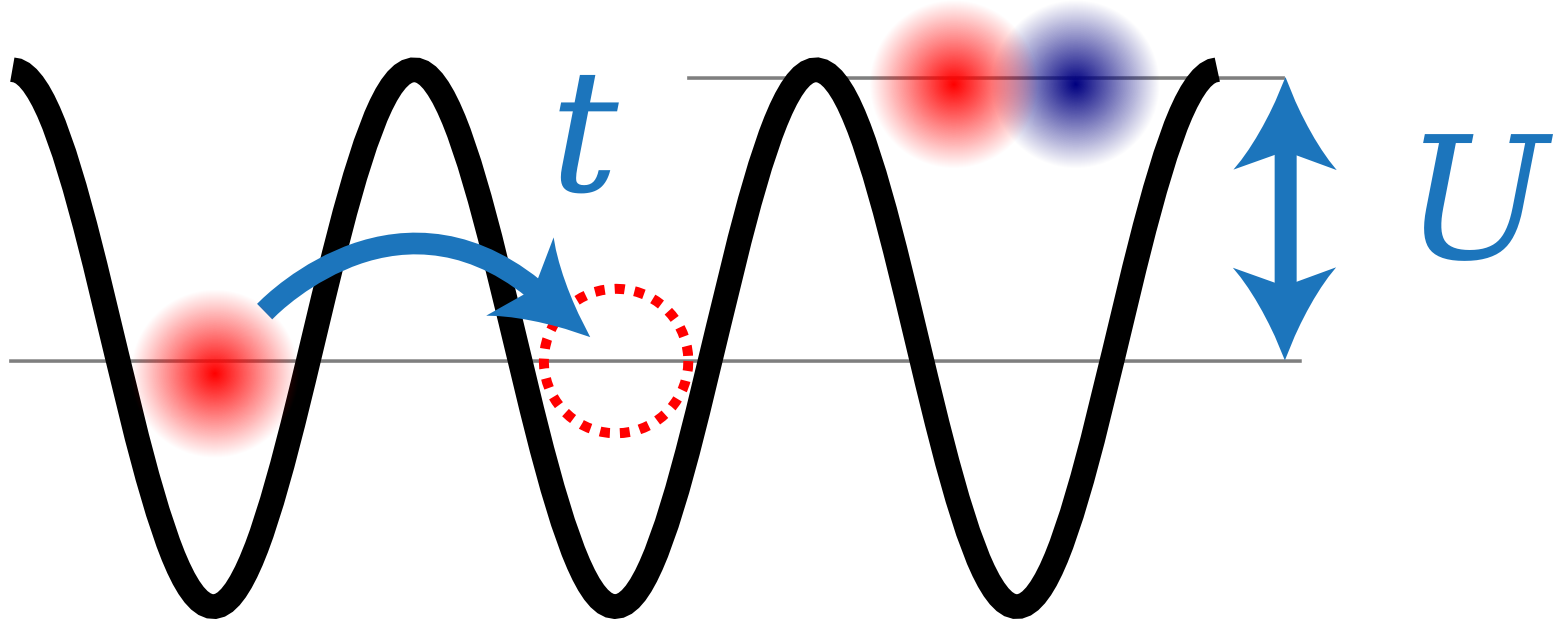
\includegraphics[width=0.4\textwidth]{../figures/hubbard/little-hubbard.png}
\caption[Hubbard model]{\small Illustration of the Hubbard model }
\label{fig:chap01hubbard}
\end{figure}
The Hubbard model is an extension of the tight-binding model, with the
interactions between electrons incorporated as the on-site energy $U$.
After its inception, it was shortly realized~\cite{Hubbard1964} that the model
could explain the Mott metal-insulator transition, which was observed in the
transition metal oxides even though conventional band theory predicted them to
be conductors.  Beyond its early success, the Hubbard model is now the
quintessential model for strongly correlated systems.  It is widely accepted as
the most viable candidate to explain high-$T_{c}$ superconductors from first
principles.   Despite this fact, its exact solution in more than one dimension
has evaded theorists for more than four decades~\cite{quintanilla2009strong}.

It is at this point that ultracold atoms enter the picture.   It turns out that
ultracold atoms in an optical lattice provide a faithful realization of the
Hubbard model~\cite{PhysRevLett.81.3108}, thus the properties exhibited by the
collection of atoms are in fact the solutions of the model.    In this way,
such systems can be used to map the phase diagram of the Hubbard model in what
is known as \textbf{quantum simulation}, an idea that was first proposed by
Richard Feynman in 1982~\cite{feynman1982simulating}. 

In a seminal paper~\cite{PhysRevLett.81.3108}, Jaksch and collaborators  showed
that Bose-Einstein condensates of atoms loaded into optical lattices could be
used as simulators of the Bose-Hubbard model.  A few years later, the
superfluid (SF) to Mott insulator (MI) phase transition, the hallmark of the
Bose-Hubbard model, was realized experimentally~\cite{Greiner2002}, and several
detailed studies of this system have followed since then~\cite{Gemelke2009,
Jimenez-Garcia2010, Trotzky2010, Mark2011, Zhang2012}.  For bosonic systems,
the properties of the ground state are well understood
theoretically~\cite{freericks1994bosehubbard, trivedi1991mott,
PhysRevB.40.546};  however, experiments on atoms in lattices are starting to
shed light into the dynamics of these systems~\cite{Fukuhara2013}, which are
more difficult to address for theorists.  

Despite the remarkable advances with bosonic systems, the ultimate goal of
quantum simulation with ultracold atoms is to find the ground states of
theoretically intractable fermionic models, to see if these models can
reproduce the measured properties of strongly correlated electron systems.  In
this prescription for quantum simulation, the subject of most interest is
whether or not the Hubbard model can exhibit a $d$-wave superfluid state which
would validate it as the prime model for high-$T_{c}$
superconductors~\cite{Scalapino1995329,PhysRevLett.89.220407}.  In pursuit of
this goal, experiments have realized the Hubbard model with spin mixtures of
fermionic atoms, where two hyperfine levels of the atomic ground state play the
role of spin-up and spin-down states of the spin-$\frac{1}{2}$ electrons in
real compounds.  Experiments with this kind of realization of the Hubbard model
are the subject of this thesis. 

A quantum degenerate spin-mixture of fermionic atoms is prepared in a harmonic
potential and then transferred adiabatically into an optical lattice potential.
The lattice depth and the contact interactions between the atoms, which
together set the values for the Hubbard parameters $t$ and $U$, can be
controlled almost at will by the experimenter.  The tunneling rate $t$ is
controlled  by adjusting the intensity of the lattice lasers.  The interaction
strength $U$ is controlled by setting the external magnetic field and making
use of a magnetically tunable Feshbach resonance, which offers the possibility
of realizing non-interacting samples, or samples with, arbitrarily, large
attractive or repulsive interactions\footnote{In practice it is observed that,
for some values of the interaction strength, significant three-body losses and
the associated heating rates prevent studying the equilibrium physics of the
quantum gas~\cite{PhysRevA.85.063615}.}.  The unprecedented control over the
system parameters has allowed the realization of band insulating
states~\cite{Kohl2005} and Mott insulating
states~\cite{Jordens2008,Schneider2008} with spin-mixtures of ultracold
fermionic atoms.  However, the possibility of exploring the strongly correlated
phases of the Hubbard model has not yet been realized because the required
temperatures are out of reach for current experiments.    


 
\section{Quantum magnetism with ultracold atoms }

Even though temperatures as low as $T\simeq 0.04\,T_{F}$ can be reached with
ultracold Fermi gases in a harmonic trap, these temperatures are not low enough
to allow exploration of the strongly correlated phases of the Hubbard model.
To get an idea of the temperature scales involved, we will examine a
qualitative temperature-doping 
%($T$-$x$) 
phase diagram, shown in Fig.~\ref{fig:cartoon-phasediag},  which is based on
experimental results obtained for the cuprate high-$T_{c}$
superconductors\footnote{See \cite{Damascelli2003} for a review of cuprate
superconductors, \cite{He2011} for a study of the onset of superconductivity at
optimal hole-doping, \cite{Jin2011} for the phase diagram of hole-doped cuprate
superconductors and \cite{Grant2011} for a more accessible report on the
subject.}, see Fig.~\ref{fig:cartoon-phasediag}.
\begin{figure} \centering
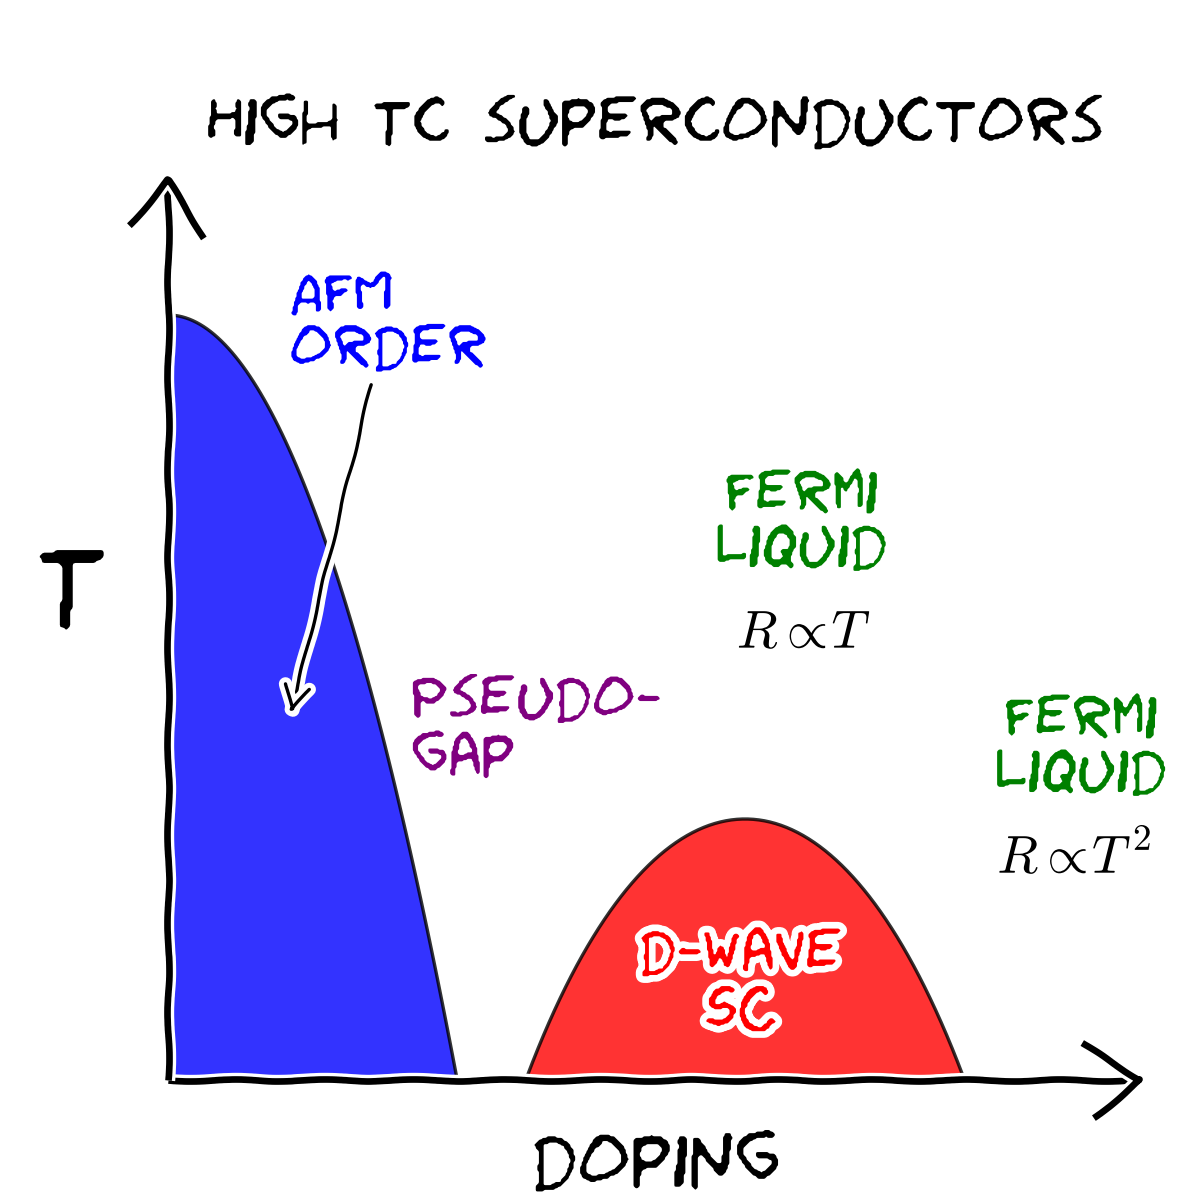
\includegraphics[width=0.4\textwidth]{../figures/hubbard/highTc.png}
\caption[Cartoon phase diagram for cuprate high-$T_{\text{C}}$
superconductors.]{\small Cartoon phase diagram for cuprate high-$T_{\text{C}}$
superconductors. The antiferromagnetic insulator (AFM) and the Fermi liquid
with quadratic resistivity are well understood by theory, however the strange
Fermi liquid with linear resistivity and the interplay between the pseudogap
regime and the superconducting dome are issues still under
debate~\cite{Grant2011}. }
\label{fig:cartoon-phasediag}
\end{figure}

The qualitative phase diagram shows that the cuprates exhibit various
interesting phases besides the superconducting (SC) dome at intermediate
doping.   Most importantly, the undoped parent compound is an antiferromagnetic
(AFM) Mott insulator with a N\'{e}el ordering temperature that is higher than
any value of the critical temperature $T_{\text{c}}$ along the SC dome.  

The onset of AFM ordering in the cuprate parent compounds is driven by the
magnetic exchange interaction~\cite{Koch2012}, where a spin can lower its
energy if it can tunnel virtually to a neighboring site.  For a single band
model, the Pauli exclusion principle dictates that this is only possible if
neighboring sites have opposing spins, as in the N\'{e}el AFM state.  The
N\'{e}el temperature $T_{N}$ is then of the order of the exchange energy
$4t^{2}/U$, which is the second-order correction (due to virtual tunneling)  to
the ground state energy of a two-site model in which the interaction $U$ is
treated as a perturbation.   The undoped parent compounds, at temperatures
several times larger than $T_{N}$, will be interaction driven Mott insulators
with exactly one electron per lattice site but without any spin ordering.  As
$T_{N}$ is approached, AFM correlations between the spins start to develop.  

To put some estimates on the values of $T_{N}$ and $T_{c}$, let's consider the
most common high-$T_{c}$ superconductor~\cite{Milton2010},
YBa$_{2}$Cu$_{3}$O$_{6+x}$, usually referred to as YBCO.  The critical
temperature for YBCO can be as large as $T_{c}\simeq 93$~K, obtained for
optimal hole-doping~\cite{Wu1987}. In the absence of doping, the YBCO parent
compound is antiferromagnetic with a N\'{e}el temperature $T_{N} \simeq 500
K$~\cite{Tranquada1988}.  The Fermi energy for YBCO is on the order of $\sim
1$~eV~\cite{liang2008ybco}, which corresponds to $\sim 10000$~K.  In units
of the Fermi temperature $T_{F}$, we have $T_{\text{C}}\simeq0.01\,T_{F}$,
and  $T_{\text{N}}\simeq0.05\,T_{F}$.

We immediately see that, in units of $T_{F}$,  the relevant temperature for
$d$-wave superconductivity is much lower than state-of-the-art temperatures for
ultracold fermionic atoms.  On the other hand $T_{N}$ may be just within reach.
The Mott insulator state (without spin ordering) was first realized with
fermionic atoms in a simple cubic lattice in
2008~\cite{Jordens2008,Schneider2008}.  Immediately after that, the race
started to see which group could be the first to observe the AFM state and take
the next step in the roadmap of quantum simulation.   

Recently in 2013, the Esslinger group, at ETH Z\"{u}rich, has demonstrated the
use of a dimerized optical lattice to measure the nearest-neighbor spin
correlations that start to develop, as a consequence of the exchange
interaction, at temperatures a few times larger than the N\'{e}el temperature
for AFM ordering~\cite{Greif2013}.  They observe significant spin-spin
correlations in arrays of one-dimensional chains, and they can detect the spin-spin
correlations that form on the approach to AFM order in a simple cubic lattice.
Prior to the work of the Esslinger group, the Bloch group used  a similar
optical super-lattice to study exchange interactions with bosons in isolated
double-wells~\cite{Trotzky2008} and isolated four-site
plaquettes~\cite{Nascimbene2012}. 

Other experiments have realized AFM states in engineered Ising Hamiltonians,
using trapped ions~\cite{Kim2010,Britton2012}, or by mapping motional degrees
of freedom to effective Ising models~\cite{Simon2011, Struck19082011}.  In
Ising type models, the magnetic coupling (anti or ferromagnetic) is put in by
hand in the Hamiltonian, and thus they realize what is referred to as
``classical'' magnetism.  In the Hubbard model, on the other hand,  magnetism
arises from the exchange interaction, as it does in condensed matter systems
such as the transition metal oxides or the cuprate parent compounds.
Realizations of classical magnetism are excellent systems to study magnetic
frustration, or the dynamics of quenching the system across a
phase-transition~\cite{PhysRevLett.111.053003}.   Systems of trapped ions can
help understand models with long range interactions~\cite{Richerme2014}, and
also emerge as good candidates to realize universal quantum
computers~\cite{Britton2012}.  Despite their advantages in other areas,
however, these systems do not directly address the long-standing open question
of superconductivity in the Hubbard model.


Approximately eight years ago, the Hulet lab started an experiment to study
strongly correlated matter using ultracold atoms in optical lattices; our main
goal being the achievement of temperatures below the N\'{e}el transition
temperature.  The N\'{e}el state in the Hubbard model,  besides being a
natural stepping stone in the quest to simulating strongly correlated systems,
offers the added benefit that it is well understood by theory~\cite{Paiva2011,
Fuchs2011}.   The ability to compare experimental results with theory offers a
test bed for quantum simulation and also a way to establish absolute
thermometry for ultracold atoms in optical lattices,  which is another major
challenge in this field~\cite{McKay2011}.  


%The absence of doping in the condensed matter system is
%equivalent to having a density of one atom per site in the ultracold atom
%system, also typically referred to as half-filling since the energy band has a
%total capacity of two atoms per site.  
%%The energy band has a total capacity of two atoms per site, so this $x=0$
%%point in the phase-diagram is also referred to as half-filling.   
%At half-filling, numerical approaches to the Hubbard model, such as
%determinantal quantum Monte Carlo (DQMC)~\cite{Paiva2011},  and dynamical mean
%field theory (DMFT)~\cite{Fuchs2011} do not suffer from the fermion sign
%problem~\cite{Jr1990}, and calculations can be performed down to temperatures
%below the N\'{e}el temperature for AFM ordering. 

\section{This thesis}

Over the course of this work we have used a compensated lattice potential,
which allows excellent control over the density distribution of the atoms in
the lattice.  The compensated lattice also helps mitigate heating of the atoms
as they are loaded into the lattice and has allowed us to reach temperatures as
low as 1.4~$T_{N}$, which is a factor of 2 colder than previous
experiments~\cite{Imriska2014}.  We measure the temperature of the atoms in the
lattice using Bragg scattering of light off of the magnetic sublattices that
start forming on the approach to the N\'{e}el transition.  This technique has
been discussed before~\cite{Ted2010}, but has not until now been implemented.
A very important aspect of our work is the comparison to \textit{ab initio}
numerical simulations of the Hubbard model.   We have used results from
determinantal quantum Monte Carlo (DQMC)~\cite{Paiva2011} and from numerical
linked-cluster expansion (NLCE)~\cite{Rigol2006} calculations,  along with the
local density approximation to establish the link between light scattering and
absolute thermometry of the sample. 

\subsection{Outline}

The approach taken in this thesis is to first provide a detailed description of
the condensed matter physics background which motivates our experiments, before
describing the experimental procedures and results.    

\begin{itemize}

\item Chapter~2 explains how ultracold atoms in an optical lattice can be an
almost ideal realization of the Hubbard model.   

\item Chapter~3 explores the
physics of the Hubbard model and gives the reader a flavor of the physics that
will be explored later on when discussing the results of our experiments. 

\item Chapter~4 introduces the experimental setup, to provide the context for the more detailed explanations that will follow.   

\item Chapter~5 discusses the optical lattice potential in which our
experiments are carried out.  We designed this potential with a few ideas in
mind regarding how it may help us reach lower temperatures with atoms in a
lattice.   Suggestions for future improvements of the setup will be given there.   

\item Chapters~6-9 describe the diagnostic tools that we have improved and
developed, over the course of this work, to access the physical observables in
our system.  

\item Chapter~10 gives details of a few crucial experimental steps required to
produce an ultracold gas of atoms in an optical lattice. 

\item Chapters 11 and
12 discuss the main results of this thesis:  the observation of an
incompressible Mott insulator of ultracold atoms in an optical lattice, and the
observation of antiferromagnetic correlations using Bragg scattering of light.

\item Chapter 13 concludes this thesis and discusses possible directions for
future experiments.  

\end{itemize}





%%%%%%%%%%%%%%%%%%%%%%%%%%%%%%%%%%%%%%%%%%%%%%%%%%%%%%%%%%%%%%%%%%%%%%%%%%%%%%%
%%%%%%%%%%%%%%%%%%%%%%%%%%%%%%%%%%%%%%%%%%%%%%%%%%%%%%%%%%%%%%%%%%%%%%%%%%%%%%%
%%%%  CHAPTER 2 
%%%%%%%%%%%%%%%%%%%%%%%%%%%%%%%%%%%%%%%%%%%%%%%%%%%%%%%%%%%%%%%%%%%%%%%%%%%%%%%
%%%%%%%%%%%%%%%%%%%%%%%%%%%%%%%%%%%%%%%%%%%%%%%%%%%%%%%%%%%%%%%%%%%%%%%%%%%%%%%

\chapter{Ultracold atoms in optical lattices}
\label{chap:atomsinlattices}

In this chapter we consider the description of cold atoms in an optical lattice
potential.    Second quantization is introduced, and the many-body Hubbard
Hamiltonian is derived, thus making the case for ultracold atoms as a nearly
ideal realization of the Hubbard model.  
% along the way we give a brief reminder of the treatment of interactions in
% cold atom gases.   
We discuss the requirements necessary for the ultracold atom system to be well
described by a single band Hubbard model. 

The computer code used to generate all of the plots in this chapter and to
calculate the Hubbard parameters $t$ and $U$ can be downloaded
from~\cite{PedroMDuarte:11612}. 


\section{One-dimensional optical lattice potential}

The contents of this section follow the derivation found in \S\,IV.A of the
review article by Morsch and Oberthaler.  \cite{RevModPhys.78.179}.  The
Hamiltonian for an atom moving in a one-dimensional (1D) sinusoidal potential,
such as that produced by an optical lattice, is 
\begin{equation}
  H_{\text{single,1D}} = 
  - \frac{\hbar^{2}}{2m} \frac{\partial^{2}}{\partial x^{2}} 
  + \vo\sin^{2}(kx) 
 \label{eq:Hsingle1D}
\end{equation}
where $k=2\pi/\lambda$, $\lambda$ is the wavelength of the lattice laser, and
$m$ is the mass of an atom.  The lattice depth \vo\ is naturally expressed in
units of the recoil energy: $\er=\frac{\hbar^{2}k^{2}}{2m}$.  Defining
$\vvo=\vo/\er$ the Hamiltonian reduces to  
\begin{equation}
\begin{split}
  H_{\text{single,1D}}= &
    -\frac{1}{k^{2}} \frac{\partial^{2}}{\partial x^{2}} 
    + \vvo\sin^{2}(kx) \\
           = &
    -\frac{1}{k^{2}} \frac{\partial^{2}}{\partial x^{2}} 
    + \frac{\vvo}{4}(2 - e^{2ikx} - e^{-2ikx} )  \\
\end{split}
\end{equation}
The solutions to the time independent Schr\"{o}dinger equation for this
Hamiltonian are Bloch states, which are labeled by their quasimomentum $q$ and
their band index $n$, and can be written in general form as 
\begin{equation}
  \psi_{q}^{n}(x) = e^{iqx} \sum_{l \in \mathbb{Z}} c_{ql}^{n} e^{ilGx}
  \label{eq:blochstate}
\end{equation}
The lattice translation invariant function that accompanies $e^{iqx}$ in a
Bloch state has been written here, with no loss of generality, as a sum of
plane waves with momenta $lG$,  where $l$ is an integer, $G=2k=2\pi/a$  is the
magnitude of the primitive vector of the reciprocal lattice,  and $a=\lambda/2$
is the lattice spacing. 

Acting with the Hamiltonian on the Bloch states and then rearranging some of
the terms in the infinite sum, we get \begin{equation}
\begin{split}
  H_{\text{single,1D}} \psi_{q}(x) = &  
      \sum_{l} \left[(q/k+2l)^{2} 
      + \frac{\vvo}{4}(2-e^{2ikx}-e^{-2ikx}) \right]
      c_{ql}^{n} e^{iqx+il2kx} \\ 
                                  = &  
      \sum_{l} \left[ \left(  (q/k+2l)^{2} 
      + \frac{\vvo}{2} \right) c_{ql}^{n} 
      - \frac{\vvo}{4}c_{q,l-1}^{n} - \frac{\vvo}{4}c_{q,l+1}^{n} \right] 
      e^{iqx+il2kx} 
\end{split}
\end{equation}
The quasimomentum is restricted to the first Brillouin zone, which can be taken
to be $[-\frac{\pi}{a}, \frac{\pi}{a})$.  The natural unit for the
quasimomentum is $2\pi/a$ ($=2k$).  Defining $q'=q/(2k)$,  we can then write
the time-independent Schr\"{o}dinger equation as 
\begin{equation}
  \left(  (2q'+2l)^{2} + \frac{\vo}{2} \right) c_{ql}^{n}
  - \frac{\vo}{4}c_{q,l-1}^{n} - \frac{\vo}{4}c_{q,l+1}^{n} = E_{q} c_{ql}^{n} 
\end{equation}
We then have an infinite linear system of equations which determines the
$c_{ql}^{n}$. For our practical purposes we truncate the set of equations such
that $|l|\leq\mathcal{N}$.  The resulting equations can be written in matrix form,
for example if we select $\mathcal{N}=2$ 
\begin{equation}
\left[\begin{smallmatrix}\frac{1}{2} V_{{0}} + 4 \left(q -2\right)^{2} & -
\frac{1}{4} V_{{0}} & 0 & 0 & 0\\- \frac{1}{4} V_{{0}} & \frac{1}{2} V_{{0}} +
4 \left(q -1\right)^{2} & - \frac{1}{4} V_{{0}} & 0 & 0\\0 & - \frac{1}{4}
V_{{0}} & \frac{1}{2} V_{{0}} + 4 q^{2} & - \frac{1}{4} V_{{0}} & 0\\0 & 0 & -
\frac{1}{4} V_{{0}} & \frac{1}{2} V_{{0}} + 4 \left(q + 1\right)^{2} & -
\frac{1}{4} V_{{0}}\\0 & 0 & 0 & - \frac{1}{4} V_{{0}} & \frac{1}{2} V_{{0}} +
4 \left(q + 2\right)^{2}\end{smallmatrix}\right] 
%
\cdot
\left[\begin{smallmatrix} 
  c_{q,-2}^{n} \\ 
  c_{q,-1}^{n} \\ 
  c_{q,0}^{n} \\ 
  c_{q,1}^{n} \\ 
  c_{q,2}^{n} \\ 
 \end{smallmatrix}\right]
 = E_{q}^{n} 
\left[\begin{smallmatrix} 
  c_{q,-2}^{n} \\ 
  c_{q,-1}^{n} \\ 
  c_{q,0}^{n} \\ 
  c_{q,1}^{n} \\ 
  c_{q,2}^{n} \\ 
 \end{smallmatrix}\right]
\label{eq:h1dmatrix} 
\end{equation}
These equations can be solved to obtain the eigenvectors $c_{ql}^{n}$ and the
eigenvalues $E_{q}^{n}$.  In the numerical solution that we implemented  we
truncated the infinite set at $\mathcal{N}=5$.  We find that, to accurately
obtain the dispersion relationship for the $n^{\text{th}}$ band, you need
$\mathcal{N}\geq n+1$.  

\subsection{Band structure}

The eigenvalues  obtained from the solutions to Eq.~\ref{eq:h1dmatrix}
correspond to the energies $E_{q}^{n}$ as a function of quasimomentum $q$ and
band index $n$ and are referred to as the band structure.  We show the band
structure for a 1D lattice as a function of $q$ in Fig.~\ref{fig:bands1d}, and
also as a function of lattice depth in Fig.~\ref{fig:bands1d_V0} 
\begin{figure}
\centering 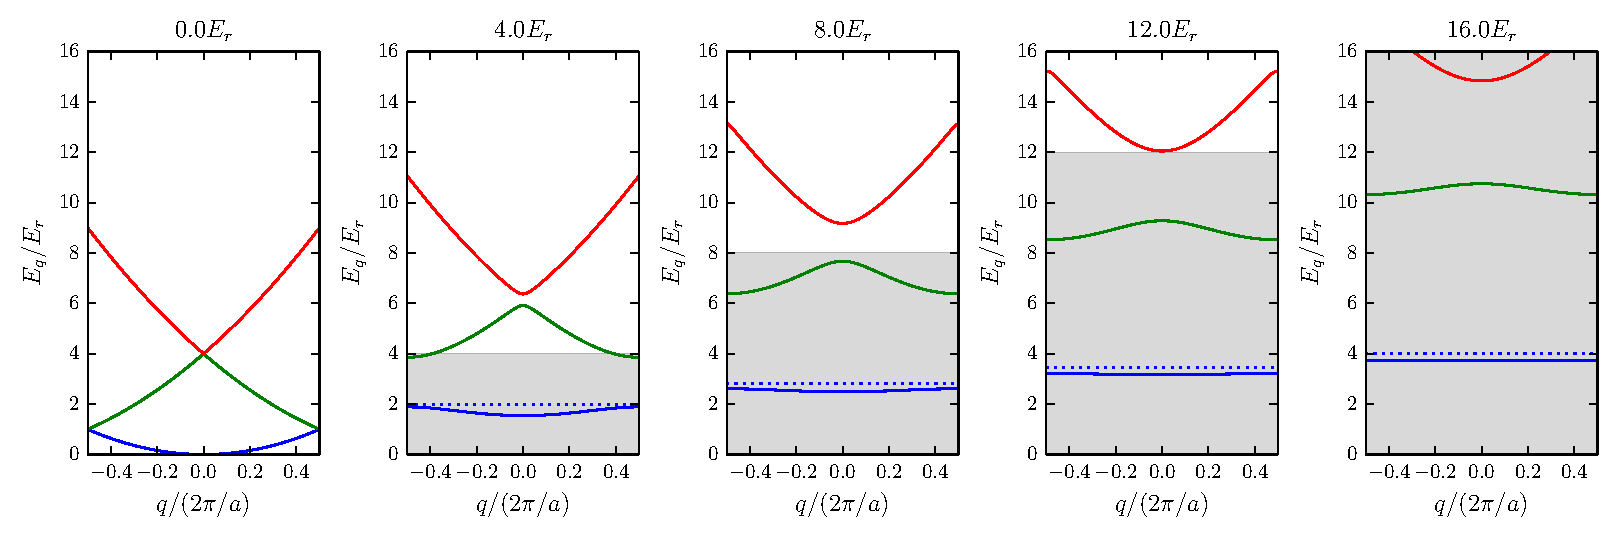
\includegraphics[width=\textwidth]{../figures/BandStructure_figures/bands1d.pdf}
\caption[Band structure in 1D lattice.]{\small Band structure in a 1D optical
lattice.  The depth of the lattice is indicated by the shaded area, and the
energy of the harmonic oscillator ground state in a single lattice site is shown
as a dotted line.  } \label{fig:bands1d}
\end{figure}
\begin{figure}
\centering 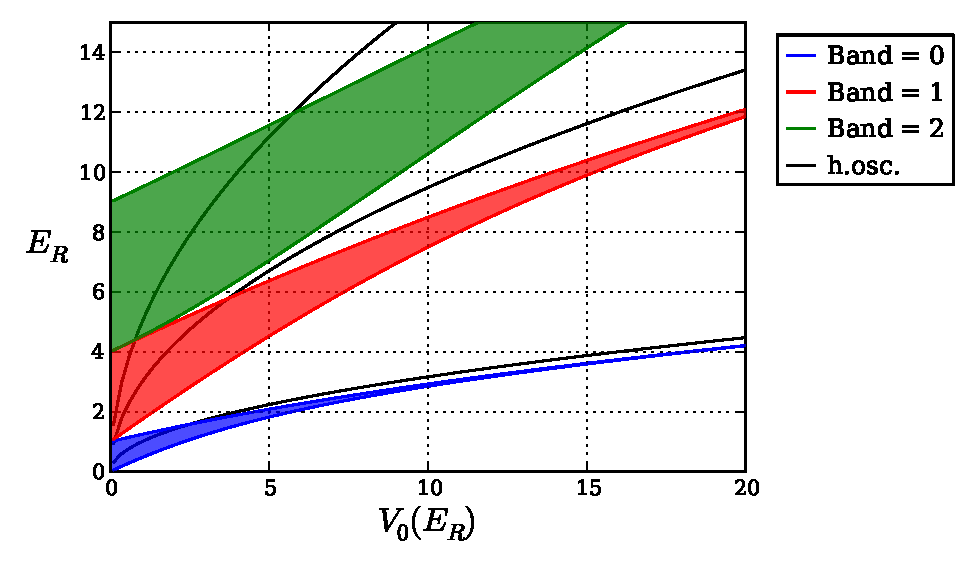
\includegraphics[width=0.6\textwidth]{../figures/BandStructure_figures/bands1d_V0.pdf}
\caption[Band structure in 1D lattice.]{\small Band structure in a 1D optical
lattice.  Each band is indicated by the colored area,  the harmonic oscillator
states in an isolated lattice site are shown as black lines. }
\label{fig:bands1d_V0}
\end{figure}

The time independent Schr\"{o}dinger equation for the Hamiltonian in
Eq.~\ref{eq:Hsingle1D}, can also be solved using Mathieu functions.  One can
then calculate the band structure by using the known properties of the Mathieu
functions, which are available on tables or as functions in some software
packages (e.g. Mathematica), see for instance the treatment
in~\cite{PhysRev.87.807}. 

\subsection{Eigenstates}
For each energy eigenvalue we have an associated eigenstate  which is defined
in terms of the $c_{ql}^{n}$ by Eq.~\ref{eq:blochstate}.   Typically, numerical
diagonalization routines return the normalized eigenvectors of the matrix in
question,  and for us this means that the coefficients $c_{ql}^{n}$ will
satisfy
\begin{equation}
   \sum_{l} | c_{ql}^{n} |^{2} = 1 
\end{equation} 
This has the implication that the states obtained from Eq.~\ref{eq:blochstate}
will be normalized over a lattice site.  In Fig.~\ref{fig:eigenfuns1d}. we show
the probability density for a lowest band eigenstate as a function of position
in the lattice for various lattice depths.  One can see how, as the lattice
gets deeper, the state becomes more localized around the center of each lattice
site. 
\begin{figure}
\centering 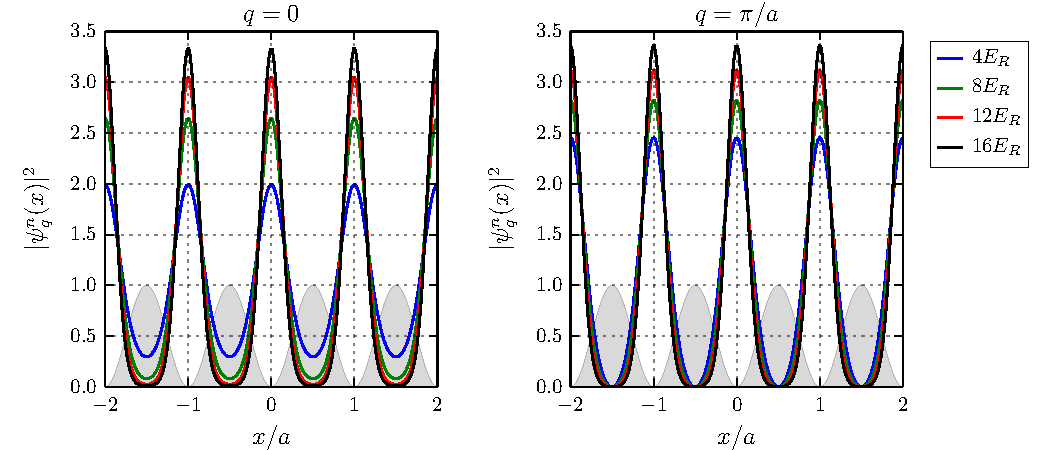
\includegraphics[width=\textwidth]{../figures/BandStructure_figures/eigenfuns1d.pdf}
\caption[Eigenstates in 1D lattice.]{\small Eigenstates of the Hamiltonian in a
1D optical lattice shown for $q=0$ (left) and $q=\pi/a$ (right) for various
lattice depths. The states are normalized so that the integral of the
probability density over one lattice site is equal to one.  The gray shaded
region is shown to indicate the variation of the lattice potential. }
\label{fig:eigenfuns1d}
\end{figure}

\subsection{Wannier states} 
\label{sec:1Dlattice}

It is useful to define a basis of states that are localized around a single
lattice site.  We will see later on that, when using such a basis, the
Hamiltonian for the Hubbard model takes its most familiar form.  In a finite
sized lattice with $L$ sites,  the localized state centered around the
$j^{\text{th}}$ site(at $x_{j}$) can be constructed as the following
superposition of eigenstates of the Hamiltonian\footnote{In some treatments
(for instance~\cite{salomon2013many}) the Wannier function is defined with a
normalization factor of $\sqrt{L}$  rather than $L$ as shown here.   Those
treatments consider eigenfunctions $\psi_{q}^{n}(x)$ which are normalized when
integrating over the full extent in the lattice.  We stick to the $L$
normalization factor, without the square root, since the eigenfunctions that
are obtained numerically come out normalized over a lattice site, as was
explained in the previous section.}: 
\begin{equation} w^{n}(x-x_{j}) =  \frac{1}{L} \sum_{q}  e^{-i q 2\pi x_{j} }
\psi_{q}^{n}(x) \label{eq:wannier} 
\end{equation} 
Here the sum runs over the
set of quasimomenta  $q \in \left\lbrace \frac{2\pi u}{a L} \ |\  u \in \lbrace
0,1,\ldots L-1 \rbrace \right\rbrace$.  Inserting the expansion of
$\psi_{q}^{n}(x)$ in plane waves into the definition of the Wannier state we
obtain 
\begin{equation}
 w^{n}(x-x_{j}) \equiv w_{j}^{n}(x)= 
    \frac{1}{L} \sum_{q}  
   \sum_{l \in \mathbb{Z}} 
   c_{ql}^{n} 
   e^{-i 2\pi q x_{j} }  
   e^{i 2\pi(q+l)x} 
\end{equation}
We will set $x_{j}=0$ for the calculation of the Wannier function,   Wannier
states centered at different lattice sites can be obtained by translation of
the $x_{j}=0$ solution. 
\begin{equation}
  w_{0}^{n}(x)= 
    \frac{1}{L} \sum_{q}  
   \sum_{l \in \mathbb{Z}} 
   c_{ql}^{n} 
   e^{i 2\pi(q+l)x} 
\end{equation}
Since the Hamiltonian commutes with the parity operator, it is required that
$\psi_{q}^{n}(-x) = \pm \psi_{q}^{n}(x)$, which implies that $c_{ql}^{n} = \pm
c_{pl'}^{n}$ if  $(q+l) = -(p+l')$.  Using this symmetry, the Wannier state
can be written as 
\begin{equation}
  w_{0}^{n}(x)= 
    \frac{1}{L} \left(
   c_{00}^{n} + 
    \sum_{q>0} 
   \sum_{l > 0 } 
   c_{ql}^{n} \left[ e^{i 2\pi(q+l)x} \pm e^{-i 2\pi(q+l)x } \right] \right)
\end{equation}
It is shown in~\cite{Kohn1959} that the maximally localized Wannier states are
obtained if the plus sign is chosen for even bands and the minus sign is chosen
for odd bands.  So, the $x_{j}=0$ Wannier state is symmetric for the even bands
and antisymmetric for the odd bands.  
\begin{equation}
  w_{0}^{n}(x)= 
    \frac{c_{00}^{n}}{L}
   + 
    \frac{2}{L}
    \sum_{q>0} 
   \sum_{l > 0 } 
   c_{ql}^{n} 
\begin{cases}
\cos[ 2\pi(q+l)x ] & \text{if $n$ even} \\
\sin[ 2\pi(q+l)x ] & \text{if $n$ odd }
\end{cases}
\end{equation}
%For $q,l>0$ all the coefficients $c_{ql}^{n}$ will have the same sign, so we
%select them to be positive.  

After defining the way to construct the Wannier states starting from the
$c_{ql}^{n}$, we can now proceed to add up the plane waves to  obtain the
states, as shown in Fig.~\ref{fig:wannier1d_V0} for various lattice depths.  As
the lattice depth is increased, the Wannier states become more localized, which
leads to less overlap between states in adjacent sites, and results in a
reduction of the probability amplitude for a particle to tunnel from one site
to the neighboring one.   More localized states also imply that the on-site
interaction will be larger, since, on average, two particles in the same site
will be closer to each other.  
\begin{figure}
\centering
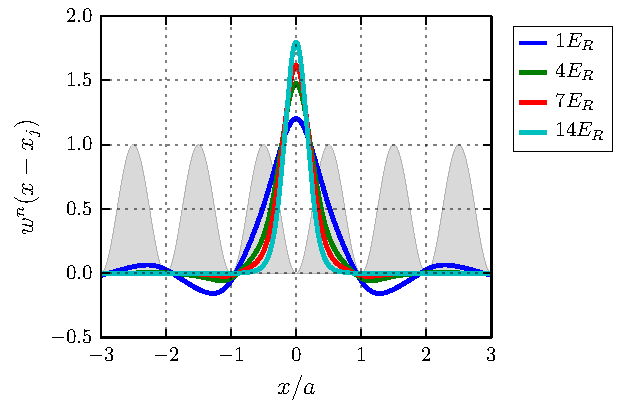
\includegraphics[width=0.6\textwidth]{../figures/BandStructure_figures/wannier1d_V0.pdf}
\caption[Wannier states in 1D lattice for various lattice depths.]{\small
Wannier states localized at $x_{j}=0$ in a 1D optical lattice for various
lattice depths.  The gray shaded region is shown to  indicate the spatial
variation of the lattice potential.  } \label{fig:wannier1d_V0}
\end{figure}

We also show, in Fig.~\ref{fig:wannier1d_bands}, the Wannier functions for the
first three bands in a 4$E_{R}$ lattice.  
\begin{figure}
\centering
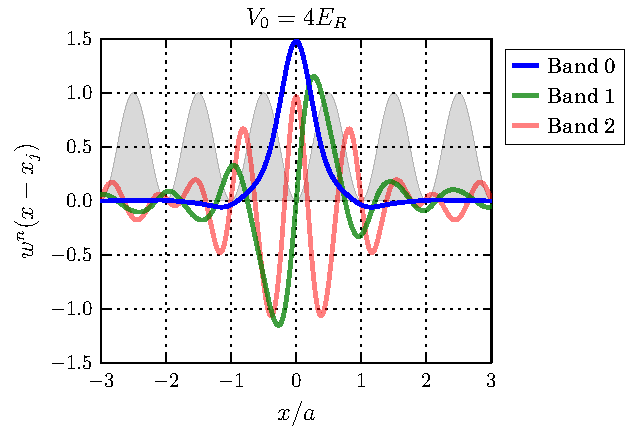
\includegraphics[width=0.6\textwidth]{../figures/BandStructure_figures/wannier1d_bands.pdf}
\caption[Wannier states in 1D lattice for the first three energy bands.]{\small
Wannier states localized at $x_{j}=0$  in a 4$E_{R}$ 1D optical lattice for the
first three energy bands.  The gray shaded region is shown to  indicate the
spatial variation of the lattice potential.  } \label{fig:wannier1d_bands}
\end{figure}

\section{Three-dimensional optical lattice potential}

The Hamiltonian for an atom moving in a  3D lattice can be separated in the
three spatial coordinates.  So we can use the solutions that were obtained in
the previous section for the 1D lattice and obtain the band structure and the
Wannier states for the 3D lattice.   The 3D band structure is shown in
Fig.~\ref{fig:bands3d_V0}. 
\begin{figure}
\centering 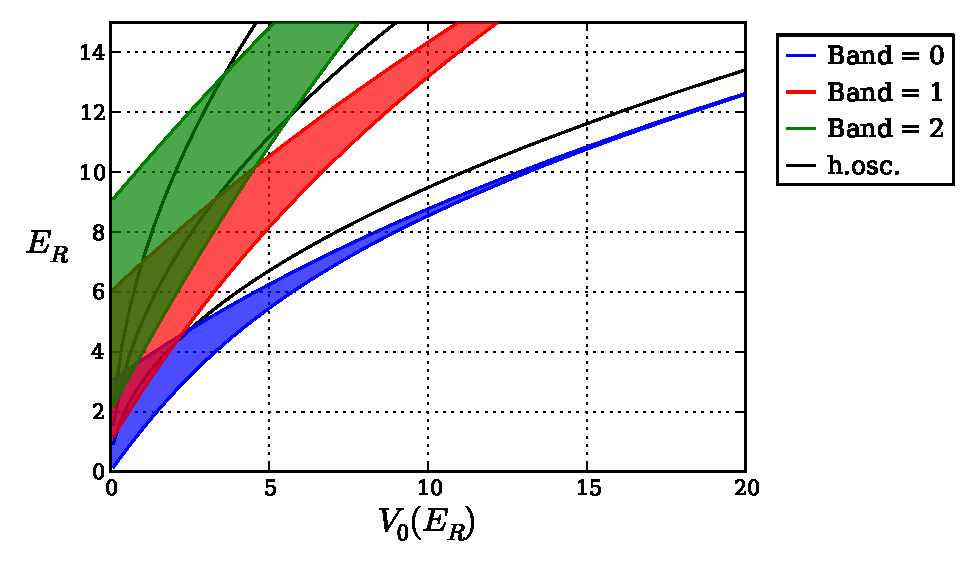
\includegraphics[width=0.6\textwidth]{../figures/BandStructure_figures/bands3d_V0.pdf}
\caption[Band structure in 3D lattice.]{\small Band structure in a 3D optical
lattice.  Each band is indicated by the colored area,  the harmonic oscillator
states in an isolated lattice site are shown as black lines. }
\label{fig:bands3d_V0}
\end{figure}

The Wannier states in a 3D lattice are simply products of the Wannier states in
each of the three spatial coordinates.  They are defined as 
\begin{equation}
 w^{n}(\bv{r}-\bv{r}_{j}) =  \frac{1}{L^{3}} \sum_{\bv{q}} e^{-i \bv{q}\cdot\bv{r}_{j} }
     \prod_{u=x,y,z}  \psi_{q_{u}}^{n_{u}}(u) 
 \label{eq:wannier3D}
\end{equation}
where $L^{3}$ is the total number of sites in the lattice. 

\section{Hubbard Hamiltonian}

The many-body Hubbard Hamiltonian is 
\begin{equation}
  H =  
-t \sum_{ \langle ij \rangle, \sigma   } 
          a_{i\sigma}^{\dagger}a_{j\sigma} \\
         + U\sum_{i} n_{i\spup} n_{i\spdn}  
\end{equation}
where $i,j$ are indices that run over lattice sites, $\langle ij \rangle$
denotes nearest-neighbors, and $\sigma$ denotes the spin state of the
particles.  The particle creation and annihilation operators,  $a_{j\sigma}$
and $a_{i\sigma}^{\dagger}$,  along with the number operator $n_{i\sigma}$
arise naturally in the second quantization formalism. In what follows, we will
see how to obtain this many-body form of the Hamiltonian, starting from the
first quantized version for a system of $N$ particles moving in a periodic
lattice. 


The Hamiltonian for a single atom in a 3D optical lattice is given by  
\begin{equation}
  H_{\text{single,3D}} = - \frac{\hbar^{2}}{2m} 
                 \left( \frac{\partial^{2}}{\partial x^{2}}
                            + \frac{\partial^{2}}{\partial y^{2}}
                            + \frac{\partial^{2}}{\partial z^{2}} \right)
 + \vo\left( \cos^{2}(kx)  + \cos^{2}(ky) + \cos^{2}(kz) \right)
\end{equation}
and when $N$ particles are considered, along with their interactions it takes a
more complicated form 
\begin{equation}
\begin{split}
  H = & \sum_{l}^{N}\left[ 
  -\frac{\hbar^{2}}{2m} \left( \frac{\partial^{2}}{\partial x_{l}^{2}}
                            + \frac{\partial^{2}}{\partial y_{l}^{2}}
                            + \frac{\partial^{2}}{\partial z_{l}^{2}} \right)
 + \vo\left( 
        \cos^{2}(kx_{l})  + \cos^{2}(ky_{l}) + \cos^{2}(kz_{l}) 
      \right) \right]\\
      &  + \frac{1}{2}\sum_{ l,n, l\neq n}^{N} 
              V_{\mathrm{int}}(\bv{r}_{l},\bv{r}_{n} )\\ 
    \equiv & ~ H_{0} + H_{\text{int}}
 \label{eq:hubbard1st}
\end{split} 
\end{equation} 
where the particles are labeled by indices $l$,$n$ and $V_{\mathrm{int}}$ is
the potential energy of interaction between two particles.  In the last line we
have defined a more concise notation that splits the Hamiltonian into the
non-interacting ($H_{0}$) and interacting ($H_{\text{int}}$) parts. Solving
this problem is a daunting task primarily for two reasons:
\begin{enumerate}
    \item The Bose or Fermi statistics of the identical particles under
consideration require the solutions to be fully symmetric or antisymmetric with
respect to particle exchange.
 
    \item The interactions between the particles prevent a straightforward
reformulation of the problem as a collection of easier-to-solve single particle
Hamiltonians.  
\end{enumerate}

The formalism of many-body theory encapsulates a series of methods to deal with
the two issues mentioned above.   First, the reformulation of the Schrodinger
equation in the language of second quantization provides the advantage that the
statistics are automatically taken into account by the notation, so one can
essentially forget about the the (anti)symmetrization of the many-particle wave
functions.  The small price to pay is that one needs to be very careful and
consistent about the order in which operators show up in the notation, since
the symmetry properties of the resulting states are contained in the
commutation relations defined between the operators.  Furthermore, second
quantization makes it easy to consider the extended Hilbert space where the
number of particles is not fixed, known as the Fock space. 

For weak interactions, many-body theory provides a solution to the problem in
terms of perturbation expansions for the physical quantities of interest.   The
theoretical formalism also reduces most of the important physical quantities in
terms of certain matrix elements (Green's functions). This allows the user to
concentrate on obtaining such matrix elements, which serve as a starting point
for the exploration of the properties of any system.   The complication arises
when the interactions are not weak, and the perturbative approach of the
many-body formalism breaks down.   


\subsection{Second quantization}

%The contents of this section comprise a short summary of the treatment in the
%books by Fetter and Walecka~\cite{fetter2003quantum} and
%Schwabl~\cite{schwabl2005advanced}.  

Let us start with a complete orthonormal set of single particle states $\lbrace
|i\rangle \rbrace \equiv \lbrace |1\rangle, |2\rangle, \ldots \rbrace$, using
these states we can write the basis states for the $N$-particle system as
\begin{equation}
   | i_{1}, \ldots i_{\alpha}, \ldots i_{N} \rangle \equiv 
   | i_{1}\rangle_{1} \ldots |i_{\alpha}\rangle_{\alpha} \ldots 
   | i_{N} \rangle_{N} ~,
\end{equation} 
which represents a state in which particle 1 is in state $i_{1} \in \lbrace
|i\rangle \rbrace$, particle $\alpha$ is in state $i_{\alpha}$ and so on.
These product states are not eigenstates of the permutation operator $P_{ij}$
which interchanges particles $i$ and $j$.  However, starting from the product
states we can obtain the completely (anti)symmetrized basis states for bosons
(fermions), which are eigenstates of any possible permutation of the
particle labels.  

For bosons, the normalized completely symmetric states are
\begin{equation} 
  | n_{1},  n_{2}, \ldots \rangle = 
  \frac{1}{\sqrt{N!n_{1}!n_{2}!\ldots}} \sum_{P}  
    P | i_{1},  i_{2}, \ldots i_{N} \rangle
\end{equation} 
where the $P$'s are elements of the permutation group\footnote{For $N$
particles there are $N!$ possible permutations and thus $N!$ elements in the
permutation group.}  In this expression, $n_{i}$ is the number of times that
the state $|i\rangle$ occurs among the $N$ particles, also called the
occupation number of state $|i\rangle$.  The sum of all occupation numbers
$n_{i}$ must equal the total number of particles, but otherwise there is no
restriction in the occupation number for bosons.

For fermions the normalized completely antisymmetric states have an extra
factor $(-1)^{P}$, which denotes the parity of the permutation $P$.  They can
be written in the form of Slater determinants: \begin{equation}
\begin{split}
  | n_{1},  n_{2}, \ldots \rangle = &
  \frac{1}{\sqrt{N!}} \sum_{P} (- 1)^{P} P |
                                 i_{1},  i_{2}, \ldots i_{N} \rangle \\
  = &
  \frac{1}{\sqrt{N!}}
  \begin{vmatrix}
  |i_{1}\rangle_{1} & |i_{1}\rangle_{2} & \dotsm & |i_{1}\rangle_{N} \\
  \vdots &  \vdots &  \ddots   & \vdots \\
  |i_{N}\rangle_{1} & |i_{N}\rangle_{2} & \dotsm & |i_{N}\rangle_{N} \\
\end{vmatrix}
\end{split} 
  \label{eq:antisymmetrize} 
\end{equation}  
If a single particle state appears more than once in the product state, the
resulting totally antisymmetric state is zero,  i.e. the occupation numbers
$n_{i}$ can only take the values 0 or 1, a consequence of the Pauli exclusion
principle. 

For bosons (fermions), we can combine the (anti)symmetric states for
$N=0,1,2,\ldots$ particles to obtain a complete orthonormal set of states for
arbitrary particle number.  This ``number states'' are the basis of the Fock
space. 


%We now define the creation  operators for bosons, which allow us to take a
%state from the subspace of $N$ particles, to the subspace of $N+1$  particles.
%\begin{equation}
% a_{i}^{\dagger} | \ldots, n_{i}, \ldots \rangle  = 
% \sqrt{n_{i}+1}|\ldots, n_{i}+1, \dots\rangle
%\end{equation}
%It follows that the adjoint of the creation operator is the annihilation
%operator and satisfies 
%\begin{equation}
%a_{i} | \ldots, n_{i}, \ldots \rangle  
%=\begin{cases}
%\sqrt{n_{i}}|\ldots, n_{i}-1, \dots\rangle
%& \text{if $n_{i}\geq 0$},\\
%0 & \text{if $n_{i}=0$}
%\end{cases}
%\end{equation}
%The creation and annihilation operators are defined such that one can create
%any state starting from the vacuum state $|0\rangle \equiv |0,0,\ldots\rangle$
%in which there are no particles at all.  In more formal terms 
%\begin{equation}
%  | n_{1}, n_{2}, \dots \rangle = \frac{1}{\sqrt{n_{1}!n_{2}!\ldots}} 
%   ( a_{1}^{\dagger} ) ^{n_{1}}  
%   ( a_{2}^{\dagger} ) ^{n_{2}}  \ldots | 0 \rangle
%  \label{eq:numberstate}
%\end{equation}
%The boson creation and annihilation operators satisfty the Bose communtation
%relations 
%\begin{equation}
%  [a_{i}, a_{j}] = 0 \ \ \ \ \  
%  [a_{i}^{\dagger}, a_{j}^{\dagger}] = 0 \ \ \ \ \   
%  [a_{i},a_{j}^{\dagger}]=\delta_{ij}
%\end{equation}

We will concentrate in the case of fermions, and define the creation operators
such that the number state can be written as 
\begin{equation}
 | n_{1}, n_{2}, \ldots \rangle = 
    \left( a_{1}^{\dagger}\right)^{n_{1}} 
    \left( a_{2}^{\dagger}\right)^{n_{2}} \ldots |0\rangle 
%    ~~~~~~ n_{i} = 0\ \text{or}\ 1  
\label{eq:defnumberstate0}
\end{equation}
where $|0\rangle$ is the vacuum state, in which there are no particles.  By
definition, the number state is completely antisymmetric, but what does this
imply for the creation operators?  Going back to Eq.~\ref{eq:antisymmetrize},
which defines the number states,  we see that the sign of the number state
depends on the particular ordering of the single particle states in the Slater
determinant.   Suppose $n_{1}=n_{2}=1$, changing the labels on states 1 and 2
corresponds to exchanging two rows in the Slater determinant and thus a minus
sign comes out: 
\begin{equation} 
    \left( a_{2}^{\dagger}\right)^{n_{2}} 
    \left( a_{1}^{\dagger}\right)^{n_{1}} \ldots |0\rangle  = 
  - | n_{1}, n_{2}, \ldots \rangle 
%    ~~~~~~ n_{i} = 0\ \text{or}\ 1  
\end{equation}
Comparing with Eq.~\ref{eq:defnumberstate0} we notice that the creation
operators must then satisfy the following anticommutation relation
\begin{equation} 
    a_{1}^{\dagger} a_{2}^{\dagger} + a_{2}^{\dagger} a_{1}^{\dagger} 
   \equiv  \left\lbrace  a_{1}^{\dagger} , a_{2}^{\dagger} \right\rbrace 
   = 0 
\end{equation}
Notice that this anticommutation relation implies $\left( a_{i}^{\dagger}
\right)^{2} = 0$, which is yet another manifestation of the Pauli exclusion
principle.
   
When dealing with fermions, one must decide first on a particular ordering of
the single particle states and then stick to it, noticing that to produce the
number states (without a minus sign) all the creation operators must be applied
to the vacuum state in the chosen order.   The action of a creation operator on
a number state is
\begin{equation}  
  a_{i}^{\dagger}| \ldots, n_{i}, \ldots \rangle 
  =    (-1)^{\sum_{k<i} n_{k}} | \ldots, n_{i}+1, \ldots \rangle 
 \label{eq:defcreation}
\end{equation} 
where the factor $(-1)^{\sum_{k<i} n_{k}}$ takes care of the number of
anticommutations needed to place the $a_{i}^{\dagger}$ operator in the correct
position.  The action of the fermion annihilation operators can be inferred by
taking the adjoint of Eq.~ \ref{eq:defcreation}.  One can then obtain all of
the anticommutation rules for fermions: 
\begin{equation}
  \left\lbrace a_{i}, a_{j} \right\rbrace = 0 \ \ \ \ \  
  \left\lbrace a_{i}^{\dagger}, a_{j}^{\dagger} \right\rbrace = 0 \ \ \ \ \   
  \left\lbrace a_{i},a_{j}^{\dagger} \right\rbrace=\delta_{ij}
\end{equation}


\subsection{Operators in second quantization}

So far two great leaps have been taken: 
\begin{enumerate}
 \item We have swept antisymmetrization under the rug by introducing the number
states, defined from the vacuum in terms of creation operators which satisfy
the Fermi anticommutation rules. 
 
 \item We started from an $N$ particle Hamiltonian, but we have now defined
number states that can handle the description of systems with an arbitrary
number of particles 
\end{enumerate}
The two ideas mentioned are related to the states used to describe the system,
now we will turn to the problem of the observables and see how they are handled
in the second quantization.  


Let us consider the sum $\sum_{\alpha} |i\rangle_{\alpha} \langle j | _{\alpha}
$ where $|i\rangle$ and $|j\rangle$ are single particle states, and $\alpha$
runs over all particles in the system.  We apply the sum to the number states
using the definition in Eq.~\ref{eq:antisymmetrize}: 
\begin{equation}
  \left(
   \sum_{\alpha} |i\rangle_{\alpha} \langle j | _{\alpha}  \right)
  | n_{1},  n_{2}, \ldots \rangle = 
  \frac{1}{\sqrt{N!}} \sum_{P} (- 1)^{P} P 
  \left( \sum_{\alpha} |i\rangle_{\alpha} \langle j | _{\alpha} 
   | i_{1},  i_{2}, \ldots i_{N} \rangle \right)
\end{equation}
For the term in the right not to vanish, the initial number state  must have a
particle in state $|j\rangle$, i.e. it must have $n_{j}=1$. Also, $n_{i}$ must
be $n_{i}=0$,  or else the completely antisymmetric state will vanish.  If the
particle initially in state $|j\rangle$ is labeled as  $J$  we can write
\begin{equation}
\begin{split}
  \left(
   \sum_{\alpha} |i\rangle_{\alpha} \langle j | _{\alpha}  \right)
  | n_{1},  n_{2}, \ldots \rangle = &
  \frac{1}{\sqrt{N!}} \sum_{P} (- 1)^{P} P \left( 
    |i_{1}\rangle_{1}
    |i_{2}\rangle_{2}
    \ldots 
     \!\!\!\!\!\!
    \underbrace{ 
    |i\rangle_{J} }_{\text{instead of } |j\rangle_{J}} 
     \!\!\!\!\!\!
    \ldots 
    |i_{N}\rangle_{N}
  \right) \\
   =&  
  \frac{1}{\sqrt{N!}}
  \begin{vmatrix}
  |i_{1}\rangle_{1} & |i_{1}\rangle_{2} & \dotsm & |i_{1}\rangle_{N} \\
  \vdots &  \vdots &     & \vdots \\
  |i\rangle_{1} & |i\rangle_{2} & \dotsm & |i\rangle_{N} \\
  \vdots &  \vdots &     & \vdots \\
  |i_{N}\rangle_{1} & |i_{N}\rangle_{2} & \dotsm & |i_{N}\rangle_{N} \\
\end{vmatrix} \\
\end{split} 
\end{equation}
In the determinant of the left, the state $|i\rangle$ appears in the
$j^{\text{th}}$ row, so a few rows need to be exchanged to put it in the
correct place, in accordance with our sign convention for the number states:
\begin{multline}
  \left(
   \sum_{\alpha} |i\rangle_{\alpha} \langle j | _{\alpha}  \right)
  | n_{1},  n_{2}, \ldots \rangle = \\  
 \begin{cases}
(-1)^{\sum_{k<j} n_{k} + \sum_{k<i}n_{k}~~~}
   \,| n_{1}, n_{2},  \ldots, n_{i}+1, \ldots,  n_{j}-1, \ldots  \rangle   
& \text{if $i\leq j$},\\
(-1)^{\sum_{k<j} n_{k} + \sum_{k<i}n_{k} -1 } 
   \,| n_{1}, n_{2},  \ldots, n_{j}-1, \ldots,  n_{i}+1, \ldots  \rangle
& \text{if $i>j$}
\end{cases}  
\end{multline}
Checking the definition of the creation and annihilation operators we obtain
the important result 
\begin{equation}
  \left(
   \sum_{\alpha} |i\rangle_{\alpha} \langle j | _{\alpha}  \right)
  | n_{1},  n_{2}, \ldots \rangle 
   =   a_{i}^{\dagger} a_{j} 
  | n_{1},  n_{2}, \ldots \rangle 
  ~~~~~ \Rightarrow ~~~~~ 
   \sum_{\alpha} |i\rangle_{\alpha} \langle j | _{\alpha} = 
     a_{i}^{\dagger} a_{j} 
\end{equation}

Now, consider an operator $T$ that is a sum over single particle operators
\begin{equation}
  T = \sum_{\alpha} t_{\alpha}
 \label{eq:defsingleparticleop}
\end{equation}  
If we insert the completeness relation for the single particle states twice in
this sum, we have \begin{equation}
\begin{split}
  T = & \sum_{\alpha} 
        \left( \sum_{i} |i\rangle_{\alpha}\langle i |_{\alpha} \right)
        t_{\alpha} 
        \left( \sum_{j} |j\rangle_{\alpha}\langle j |_{\alpha} \right) \\
    = & \sum_{ij}   \langle i | t | j \rangle  
          \sum_{\alpha} |i\rangle_{\alpha} \langle j |_{\alpha} \\ 
    = & \sum_{ij}   \langle i | t | j \rangle a_{i}^{\dagger} a_{j} 
          \equiv \sum_{ij} t_{ij}   a_{i}^{\dagger} a_{j} 
\end{split}  
\end{equation}
\textbf{This is the other big leap provided by the second quantization}:  an
operator that was written as a sum over particles becomes a sum of creation and
annihilation operators.   We will apply this prescription to the
non-interacting part of the Hamiltonian for $N$ particles moving in a lattice.  

Operators like the potential energy, $ \frac{1}{2}\sum_{l,n,l\neq n}^{N}
V_{\mathrm{int}}(\bv{r}_{l}, \bv{r}_{n} )$ , which are a sum over two-particle
(or many-particle) operators,  can be similarly expressed as sums of creation
and annihilation operators~\cite{schwabl2005advanced}.  For a two-body operator
we have the expression
\begin{equation}
\begin{split}
F = & \frac{1}{2} \sum_{\alpha\neq\beta} f(\bv{r}_{\alpha}, \bv{r}_{\beta} )  \\
  = & \frac{1}{2} \sum_{ijkm} \langle ij | f | km \rangle 
        a_{i}^{\dagger} a_{j}^{\dagger} a_{m} a_{k} 
\end{split}
\end{equation}

\subsection{Second quantized Hubbard Hamiltonian}

The Hubbard Hamiltonian in Eq.~\ref{eq:hubbard1st} is a sum of two
single-particle operators and one two-particle operator.  These are,
respectively: the kinetic energy, the energy of the atoms in the lattice
potential, and the interactions between the atoms.  In this section we will
express the Hubbard Hamiltonian in second quantized form.  As a single-particle
basis we will use the Wannier states that were derived in
Section.~\ref{sec:1Dlattice}

%In the Hubbard Hamiltonian the two single-particle operators are grouped
%together to define the non-interacting part of the Hamiltonian 
%\begin{equation}
%\begin{split}
%  H_{0} = & \sum_{l}^{N} -\frac{\hbar^{2}}{2m} 
%            \left( \frac{\partial^{2}}{\partial x_{l}^{2}}
%                            + \frac{\partial^{2}}{\partial y_{l}^{2}}
%                            + \frac{\partial^{2}}{\partial z_{l}^{2}} \right)
% + \vo\left( \cos^{2}(kx_{l})  + \cos^{2}(ky_{l}) + \cos^{2}(kz_{l}) \right) \\
%       = & \sum_{l}^{N} H_{\text{single,3D}}^{l}
%\end{split}
%\end{equation}

\paragraph{Tunneling matrix element, $\bm{t}$.} $H_{0}$ is a single particle
operator of the kind defined in Eq.~\ref{eq:defsingleparticleop}:
\begin{equation}
  H_{0} = 
     \sum_{l=1}^{N} H_{\text{single,3D}}^{l}
\end{equation}
where 
\begin{equation}
H_{\text{single,3D}}^{l} = 
  -\frac{\hbar^{2}}{2m} \left( \frac{\partial^{2}}{\partial x_{l}^{2}}
                            + \frac{\partial^{2}}{\partial y_{l}^{2}}
                            + \frac{\partial^{2}}{\partial z_{l}^{2}} \right)
 + \vo\left( \cos^{2}(kx_{l})  + \cos^{2}(ky_{l}) + \cos^{2}(kz_{l}) \right) 
\end{equation}
Its second quantized form can be written as 
\begin{equation}
\begin{split}
  H_{0} = & \sum_{ij} 
       \langle i| H_{\text{single,3D}} |j \rangle a_{i}^{\dagger} a_{j} \\
        \equiv & ~ -\sum_{ij} t_{ij}  a_{i}^{\dagger} a_{j} \\
\end{split}
\end{equation}  
Note that the sign of $t_{ij}$ was picked rather arbitrarily to follow the
usual conventions.  We now proceed to find the value of the matrix element
$t_{ij}$.  We use the definition of the Wannier states given in
Eq.~\ref{eq:wannier3D} to find 
\begin{equation}
\begin{split}
-t_{ij}  
= & 
  \frac{1}{L^{6}}\int \mathrm{d}\bv{r}\ 
     \sum_{\bv{q}'} e^{i \bv{q'}\cdot\bv{r}_{i} }
     \prod_{u'=x,y,z}  \psi_{q'_{u'}}^{n'_{u'}*}(u') 
  \Big( H_{\text{single,3D}}  \Big)
     \sum_{\bv{q}} e^{-i \bv{q}\cdot\bv{r}_{j} }
     \prod_{u=x,y,z}  \psi_{q_{u}}^{n_{u}}(u)\\ 
= &
  \sum_{\bv{q}\bv{q}'}   
  \frac{E_{\bv{q}}^{n}}{L^{6}}
   e^{ i \bv{q}'\cdot\bv{r}_{i} }  e^{ -i \bv{q}\cdot\bv{r}_{j} }
   \int\mathrm{d}\bv{r}\ 
     \prod_{u'=x,y,z}  \psi_{q'_{u'}}^{n'_{u'}*}(u') 
     \prod_{u=x,y,z}  \psi_{q_{u}}^{n_{u}}(u) \\ 
= &
  \sum_{\bv{q}\bv{q}'}   
  \frac{E_{\bv{q}}^{n}}{L^{6}}
   e^{ i \bv{q}'\cdot\bv{r}_{i} }  e^{ -i \bv{q}\cdot\bv{r}_{j} }
   \delta_{\bv{q}\bv{q}'} \delta_{nn'} L^{3} \\
= &
  \frac{1}{L^{3}}
  \sum_{\bv{q}}   E_{\bv{q}}^{n}
   e^{ i \bv{q}\cdot(\bv{r}_{i} - \bv{r}_{j}) } \delta_{nn'}\\
\end{split} 
\end{equation}
We observe that there is no amplitude to go between states that are in two
different bands, as is indicated by the appearance of $\delta_{nn'}$.   In what
follows, we will consider only the lowest band, $n=0$,  so we will drop the
band index, $n$, altogether.  For this simplification to be valid, the
following two requirements must be satisfied by the system:
 
\begin{enumerate}
\item \textbf{The temperature and the Fermi energy need to be small compared to
the energy gap between the lowest and first excited band.}

\item \textbf{The interaction energy scale must also be small compared to the
energy gap between the lowest and first excited band.}
\end{enumerate}

In the 3D lattice, the total energy $E_{\bv{q}}$ is the sum of the energy
associated with each quasimomentum component, $E_{\bv{q}} = \sum_{u=x,y,z}
E_{q_{u}} $.  By inserting this into the sum for $t_{ij}$ above we find 
\begin{multline}
-t_{ij} =  \frac{1}{L^{3}} \left[ 
          \left(\sum_{q_{x}} E_{q_{x}}   e^{ i q_{x} x_{ij} }   \right)
          \sum_{q_{y}} e^{ i q_{y} y_{ij} }   
          \sum_{q_{z}} e^{ i q_{z} z_{ij} }  
   \right. \\
\left. 
          + 
          \sum_{q_{x}} e^{ i q_{x} x_{ij} }  
          \left(\sum_{q_{y}} E_{q_{y}}   e^{ i q_{y} x_{ij} }   \right)
          \sum_{q_{z}} e^{ i q_{z} z_{ij} }  
          + 
          \sum_{q_{x}} e^{ i q_{x} x_{ij} }  
          \sum_{q_{y}} e^{ i q_{y} y_{ij} }   
          \left(\sum_{q_{z}} E_{q_{z}}   e^{ i q_{z} z_{ij} }   \right)
\right]
\end{multline}
We make use of the identity $\sum_{q_{u}} e^{ iq_{u}(u_{i}-u_{j}) } = L
\delta_{u_{i}u_{j}}$ to obtain
\begin{equation}
-t_{ij} =  \frac{1}{L} \left[ 
    \left(\sum_{q_{x}} E_{q_{x}}^{\text{\tiny 1D}}  e^{ i q_{x} x_{ij} } \right)
    \delta_{y_{i}y_{j}}
    \delta_{z_{i}z_{j}}
    + 
    \left(\sum_{q_{y}} E_{q_{y}}^{\text{\tiny 1D}}  e^{ i q_{y} x_{ij} } \right)
    \delta_{x_{i}x_{j}}
    \delta_{z_{i}z_{j}}
    + 
    \left(\sum_{q_{z}} E_{q_{z}}^{\text{\tiny 1D}}  e^{ i q_{z} z_{ij} } \right)
    \delta_{x_{i}x_{j}}
    \delta_{y_{i}y_{j}}
\right]
\label{eq:tunnelinglong}
\end{equation}

If $i=j$ we have 
\begin{equation}
  -t_{ii} =  \frac{3}{L} 
          \sum_{q} E_{q} 
\end{equation}
Since $q$ runs over the $L$ different values in the set $q \in \left\lbrace
\frac{2\pi u}{a L} \ |\  u \in \lbrace 0,1,\ldots L-1 \rbrace \right\rbrace$
(as explained above following Eq.\ref{eq:wannier}), $-t_{ii}$ is nothing more
than the mean energy of the 3D energy band, which we will refer to as
$\bar{E}$,  $-t_{ii}\equiv \bar{E}$  

If $i\neq j$,  tunneling can only occur along one of the lattice directions as
can be seen from the different Kronecker delta terms that show up in
Eq.~\ref{eq:tunnelinglong}.   In other words, for the simple cubic potential,
diagonal tunneling events are second order processes.  If we write the distance
between sites $i$,$j$ as $\Delta_{ij}$, the tunneling matrix element simplifies
to  
\begin{equation}
  -t_{ij} = \frac{1}{L} \sum_{q} E_{q} e^{iq \Delta_{ij}} 
\label{eq:tunneling3D}
\end{equation}
Formula~\ref{eq:tunneling3D} is how we regularly calculate the tunneling matrix
element\footnote{This derivation has used the Wannier states,
constructed as a sum of plane waves, to obtain the tunneling matrix element.
It can also be obtained directly from the Wannier states'  wavefunctions as:
\begin{equation}
  -t_{ij} = \int \mathrm{d}\bv{r} \, w_{i}(\bv{r}) H_{\text{single,3D}} w_{j}(\bv{r}) 
\end{equation}
Calculating the tunneling matrix element by computing the overlap integral of
the Wannier wavefunctions is computationally more expensive than obtaining it
as a sum over the energy eigenvalues of the band. }. Starting from the lattice
depth we solve for $E_{q}$ and then carry out the sum over $q$.


In the tight-binding approximation, terms for which $|\Delta_{ij}|>a$ are
neglected, and  $\Delta_{ij}$ can only take the values $-a$ or $a$,
where $a$ is the lattice spacing.  In this case we use $t_{ij}\equiv t$, where
$t$ is given by
\begin{equation}
  -t = \frac{1}{L} \sum_{q} E_{q} e^{iqa} 
\label{eq:tunneling3D_tight}
\end{equation}

We can then go ahead and write the second quantized form of $H_{0}$ in the
tight-binding approximation 
\begin{equation}
  \label{eq:hubbard_not_shifted} 
  H_{0}  =  \bar{E} \sum_{i}  a_{i}^{\dagger} a_{i}  - t 
    \sum_{ \langle i j \rangle }
                      a_{i}^{\dagger} a_{j}   
\end{equation} 
The first term in this expression is constant for a system with a conserved
number of particles, since $\sum_{i}  a_{i}^{\dagger} a_{i}=N$.    Usually this
energy offset is neglected, but when dealing with inhomogeneous systems which
have a position dependent lattice depth it will be important to take it into
account, as we will see later on.   


We can go ahead and invert the Fourier series in Eq.~\ref{eq:tunneling3D} to
obtain 
\begin{equation} 
  E_{q} = - \sum_{\Delta_{ij}} t_{ij} e^{-iq \Delta_{ij}} 
\end{equation}
which in the tight-binding approximation reduces to 
\begin{equation}
  E_{q} = -2 t\cos( qa) 
\end{equation}
This explicit form for the dispersion relation allows us to relate the
bandwidth, $W_{\text{1D}}$, to the tunneling matrix element as
$W_{\text{1D}}=4t$,  which in 3D becomes $W_{\text{3D}}= 12t$.

It is useful to find out the range of lattice depths for which the
tight-binding approximation is valid in the optical lattice potential.  To do
this we just need to look at the tunneling matrix elements for beyond
nearest-neighbor tunneling,  as shown in Fig.~\ref{fig:tightbinding}.  It is
seen in the figure that, for lattice depths $\gtrsim 5 E_{R}$  we can safely
ignore beyond nearest-neighbor tunneling, see also Fig.~\ref{fig:hubbardvalid}.  
\begin{figure}
\centering
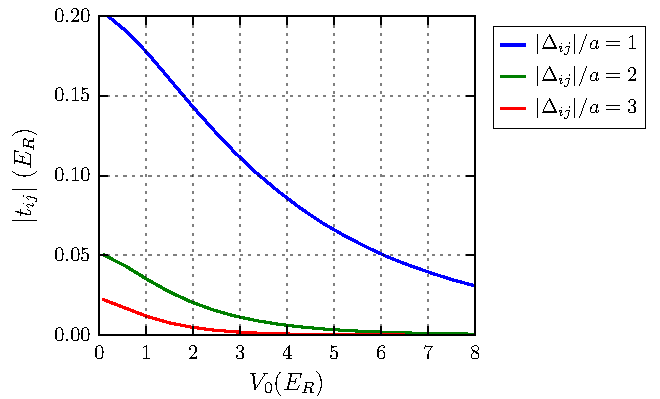
\includegraphics[width=0.6\textwidth]{../figures/BandStructure_figures/tightbinding_V0_interp.pdf}
\caption[Tunneling matrix elements in a 3D lattice.]{\small Tunneling matrix
element in an optical lattice as a function of lattice depth.  Nearest-neighbor
and beyond nearest-neighbor matrix elements are shown to illustrate the range
of lattice depths for which the tight-binding limit is a good approximation.
$\Delta_{ij}$ corresponds to the distance between initial and final lattice
sites in the tunneling matrix element.  For $V_{0}\gtrsim 5\,E_{r}$ we can
safely neglect tunneling beyond nearest neighbors.  } \label{fig:tightbinding}
\end{figure}

Yet another way of estimating the tunneling matrix element \cite{Bloch2008} is
by using the relationship $t=W_{\text{1D}}/4$, valid in the tight-binding
limit, and then working backwards.  An analytical form for the bandwidth can be
obtained from the known properties of the Mathieu functions, which are
solutions to the Schrodinger equation in a 1D lattice.  This approach yields
the analytic result 
\begin{equation}
 t/\er \simeq \frac{4}{\sqrt{\pi}} \vvo^{3/4} \exp(-2\sqrt{\vvo}) 
\label{eq:tunnelMathieu}
\end{equation} 
where \vvo\ is the lattice depth in units of the recoil energy. This formula
appears in a popular review of the subject~\cite{Bloch2008} and is thus widely
used.  The comparison between the result from Eq.~\ref{eq:tunneling3D} and
Eq.~\ref{eq:tunnelMathieu} is shown in Fig.~\ref{fig:tMathieu}. 
\begin{figure}
\centering
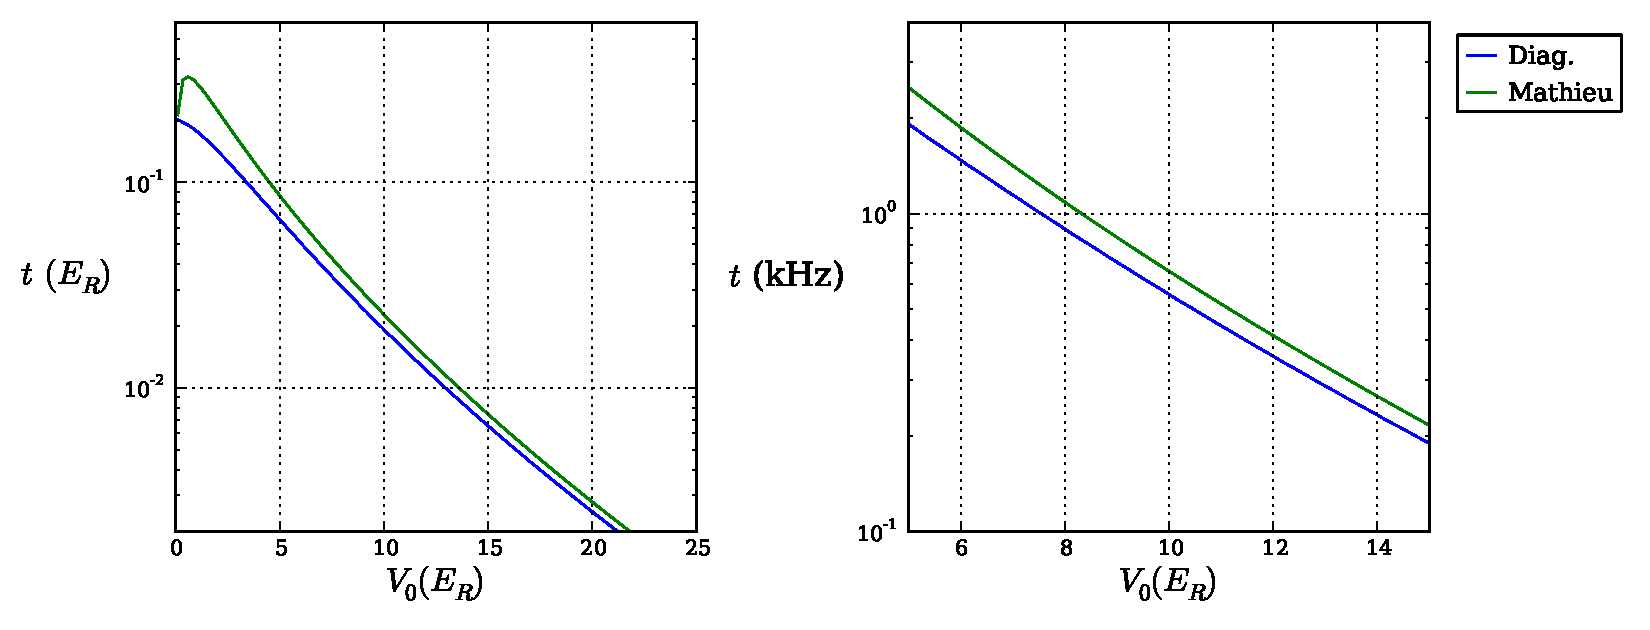
\includegraphics[width=\textwidth]{../figures/BandStructure_figures/tunneling_V0_Mathieu.pdf}
\caption[Nearest neighbor tunneling matrix element]{\small Nearest neighbor
tunneling matrix element in an optical lattice as a function of lattice depth.
Comparison between the result from Eq.~\ref{eq:tunneling3D} (blue line) and the
one obtained from the Mathieu functions, Eq.~\ref{eq:tunnelMathieu} (green
line).  The right panel shows the tunneling rate in kHz for the mass of a
$^{6}$Li atom.  At 7\,$E_{r}$, where we perform most of our experiments, the
discrepancy can be significant.  }
\label{fig:tMathieu}
\end{figure}

%Finally, we have the second quantized form of $H_{0}$ in the tight-binding
%limit 
%\begin{equation}
%  H_{0} = -t \sum_{ \langle ij \rangle } a_{i}^{\dagger}a_{j} 
%\end{equation}
%where the $\langle \rangle$ denote nearest-neighbors, and the creation operator
%$a_{i}^{\dagger}$ create particles in the Wannier state localized at site $i$.

Notice that, up to now, we have ignored the spin part of the wavefunction.   We
can include it easily by noticing that $H_{0}$ does not act on the spin at all,
so the states $|i\rangle$ and $|j\rangle$ that we have used in the derivation
above need to have the same spin.   If two spin states are available, our basis
set is twice as large, which can be taken care of by including a sum over spin
states in the second quantized form of the Hamiltonian:
\begin{equation}
  H_{0} = \bar{E}\sum_{i}  a_{i}^{\dagger} a_{i} \, -\ t
   \!\!\! 
  \sum_{ \langle ij \rangle, \sigma=\dbl   } 
   \!\!\!
  a_{i\sigma}^{\dagger}a_{j\sigma} 
\end{equation}

\paragraph{On-site interaction energy, $\bm{U}$.}

The interaction part of the Hamiltonian for $N$ particles is
given by \begin{equation}
    H_{\text{int}} = 
         \frac{1}{2}\sum_{ l,m, l\neq m}^{N} 
         V_{\mathrm{int}}(\bv{r}_{l},\bv{r}_{m} )\\ 
\end{equation}
This is a two-particle operator, and its second quantized form is given by
\begin{equation}
   H_{\text{int}} = \frac{1}{2} \sum_{i,j,k,m} 
           \langle ij | V_{\mathrm{int}} | km \rangle
           a_{i}^{\dagger} a_{j}^{\dagger} a_{m} a_{k}
\end{equation}
where 
\begin{equation}
    \langle ij | V_{\mathrm{int}} | km \rangle =
    \int \mathrm{d}\bv{r}_{1} \int \mathrm{d}\bv{r}_{2} \ \  
    \varphi_{i}^{*}(\bv{r}_{1}) \varphi_{j}^{*}(\bv{r}_{2}) 
    V_{\mathrm{int}}(\bv{r}_{1},\bv{r}_{2}) 
    \varphi_{k}(\bv{r}_{1}) \varphi_{m}(\bv{r}_{2}) 
\end{equation}
and the $\varphi$'s correspond to the wavefunctions of the single particle
basis states chosen. 

The interaction between ultracold atoms can be described in terms of the
$s$-wave scattering length, $a_{s}$,  and a
pseudo-potential~\cite{sakurai2014modern,Bloch2008} given by\footnote{This is a
good approximation as long as the $s$-wave scattering lengths is small compared
to the single-site harmonic oscillator length~\cite{Busch1998}. This condition
is typically satisfied, and other concerns such as collisional losses or
coupling to higher bands become more important well before the $s$-wave
scattering length is comparable to the harmonic oscillator length.  For
reference, the harmonic oscillator length in a lattice site is $\ell = a / (\pi
\vvo^{1/4})$, which for a 7\,\er\ lattice with $a=532\,$nm is $\ell \approx
2000\,a_{0}$, where $a_{0}$ is the Bohr radius.}
\begin{equation}
    V_{\mathrm{int}}(\bv{r}_{1},\bv{r}_{2}) 
    = \frac{ 4 \pi \hbar^{2} a_{s} } { m } \delta(\bv{r}_{1}-\bv{r}_{2}) 
\end{equation}
so the matrix element above can be written as 
\begin{equation}
    \langle ij | V_{\mathrm{int}} | km \rangle =
\frac{ 4 \pi \hbar^{2} a_{s} } { m }
    \int \mathrm{d}\bv{r}  \ \  \varphi_{i}^{*}(\bv{r}) \varphi_{j}^{*}(\bv{r}) 
                                \varphi_{k}(\bv{r}) \varphi_{m}(\bv{r}) 
\end{equation}
Our basis states, $\varphi$, are the 3D Wannier states defined in
Eq.~\ref{eq:wannier3D}, which are separable in the three spatial coordinates.
We recall that the Wannier states are labeled by the lattice site around which
they are centered, and by their band index.   If we explicitly write out the two
labels in the expression above, we obtain
\begin{equation}
    \langle ij | V_{\mathrm{int}} | km \rangle =
\frac{ 4 \pi \hbar^{2} a } { m }
  \prod_{v=x,y,z}
    \int \mathrm{d}v  \ \ 
    w_{i}^{n_{i}}(v) w_{j}^{n_{j}}(v) w_{k}^{n_{k}}(v) w_{m}^{n_{m}}(v) 
   \equiv \, U_{ijkm}
\end{equation}

In general $i,j,k,m$ can represent any lattice sites.  We will restrict
our treatment to on-site interactions by enforcing $i=j=k=m$,  furthermore, we
consider only Wannier states in the lowest band. 
%The Wannier function along  $x,y,z$ depends on the lattice depth along the
%respective coordinate.  We will consider a lattice with different depths along
%the three spatial coordinates, $\bvo = ( V_{0x}, V_{0y}, V_{0z} ) $.  At this
%point we make the approximation of neglecting all of the off-site interaction
%terms, which can be justified by the localized nature of the Wannier states.
%Furthermore, we consider only Wannier states in the lowest band, which is
%valid for scattering lengths smaller than the single-site harmonic oscillator
%length~\cite{Busch1998}.  
With this considerations, and also explicitly writing down the spin quantum
number, we find 
\begin{equation}
   H_{\text{int}} =  
           \frac{U}{2}
        \sum_{i} 
         \left( 
           a_{i\spup}^{\dagger} a_{i\spdn}^{\dagger} a_{i\spdn} a_{i\spup} +
           a_{i\spdn}^{\dagger} a_{i\spup}^{\dagger} a_{i\spup} a_{i\spdn}
         \right)\\
\end{equation}
where we have defined $U\equiv U_{ijkm}$ for $i=j=k=m$, with $U$ is given by  
%\begin{equation}
%  U = 
%  \frac{ 4 \pi \hbar^{2} a } { m }
%   \prod_{v=x,y,z}  \int  w(v) ^{4} \mathrm{d}v  
%\end{equation}
%In units of $E_{R}$, 
\begin{equation}
  U/\er = \frac{ 8}{ \pi}  \frac{ a_{s} }{a}
   \prod_{v=x,y,z}  \int  w(v) ^{4} \mathrm{d}v  
\end{equation}

Defining the number operator as $n_{i\sigma} = a_{i\sigma}^{\dagger}
a_{i\sigma}$ 
\begin{equation}
\begin{split}
   H_{\text{int}}  
     = & \  
           \frac{U}{2}
         \sum_{i} \left( 
           n_{i\spdn} n_{i\spup} + 
           n_{i\spup} n_{i\spdn} \right) 
    \\
     = & \ 
           U\sum_{i}
           n_{i\spup} n_{i\spdn}  
\end{split}
\end{equation}
where $i$ runs over all of the lattice sites.  


To calculate the value of $U$ we use the Wannier states obtained in
Sec.~\ref{sec:1Dlattice}.  Alternatively, one can approximate the Wannier state
by the Gaussian ground state in the local oscillator potential of one lattice
site and carry out the integral analytically to obtain~\cite{Bloch2008} 
\begin{equation} 
  U  = \sqrt{ 8\pi } \frac{a_{s}}{a} \vvo^{3/4} 
\end{equation} 
Figure~\ref{fig:wfactor} shows a comparison of the exact result and the
Gaussian approximation to the Wannier state for a lattice with
$\lambda=1064$\,nm. 
\begin{figure}
\centering
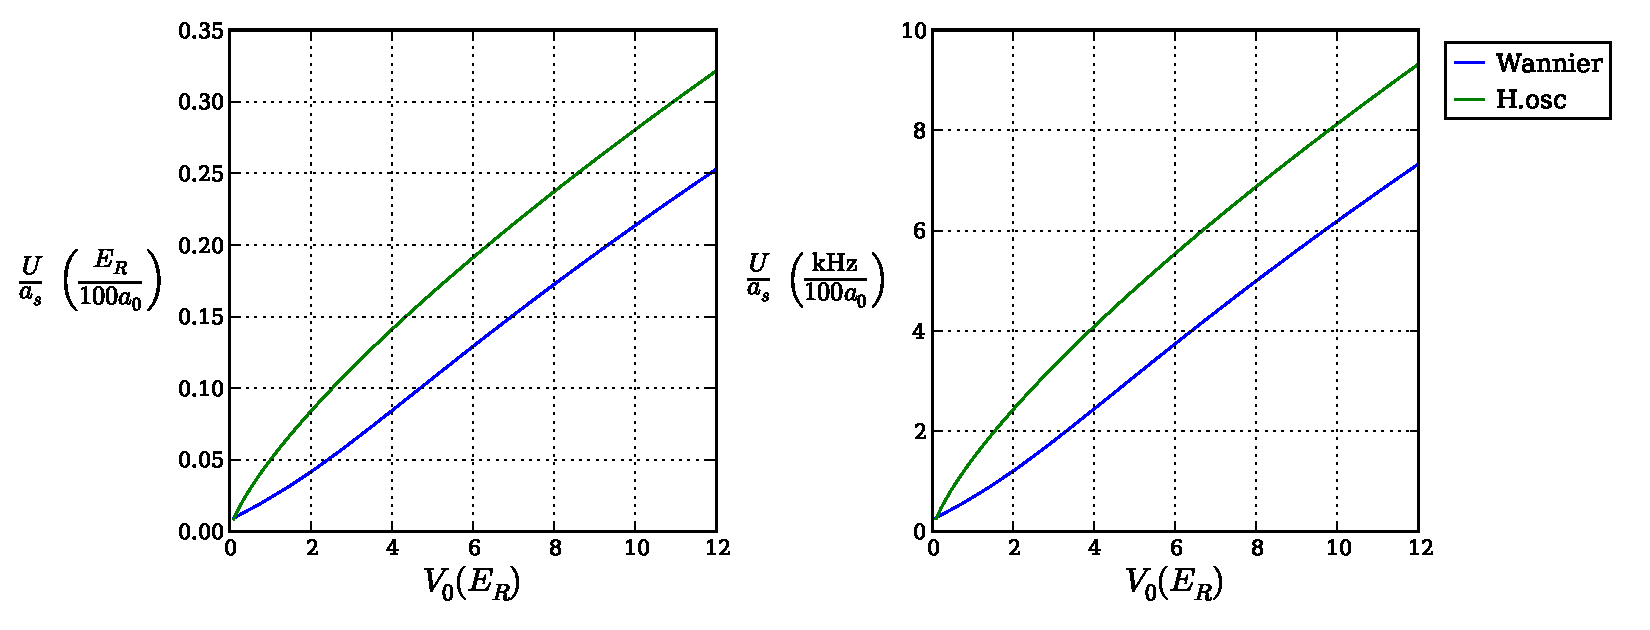
\includegraphics[width=\textwidth]{../figures/BandStructure_figures/wFactor_V0_a0.pdf}
\caption[On-site interactions in a 3D lattice]{\small On-site interactions in a
3D lattice ($\lambda=1064\,\text{nm}$) as a function of lattice depth.
Numerical calculation using Wannier functions (blue line) compared to the
approximation using harmonic oscillator states (green line).  The lattice
depth is the same in all three directions of the lattice.   The left panel
shows uses \er\ for the units of $U$ and the right panel uses kHz for $U/h$. }
\label{fig:wfactor}
\end{figure}

If the on-site interaction term is comparable to the energy spacing between the
lowest and first excited bands, the single band approximation presented here
breaks down.  Corrections to the tunneling rate and the on-site interactions
are necessary, which may depend on the lattice site
occupation~\cite{Werner2005,Jordens2010,Mark2012}.

\section{Parameter regimes for a valid description using a single band
Hubbard model}

Throughout this chapter we have mentioned the possible scenarios for which the
single band Hubbard model is not an accurate description of ultracold atoms in
an optical lattice.  The two most important ones are:
\begin{itemize} 
\item The on-site interaction $U$ is comparable to the band gap $\Delta$.  The
band gap is the energy difference between the highest energy state in the
lowest band and the lowest energy state in the first excited band, see
Fig.~\ref{fig:bands3d_V0}. \item Tunneling beyond nearest-neighbor (rate
$t_{2}\equiv t_{ij}$ for $\Delta_{ij}=2a$, see Fig.~\ref{fig:tightbinding}) is
not negligible compared to nearest-neighbor tunneling (rate $t$), i.e.  the
tight-binding approximation does not hold. 
\end{itemize}
In Fig.~\ref{fig:hubbardvalid} we have represented these two conditions as a
function of the lattice depth and the $s$-wave scattering length.  For more
details on the validity of the single band Hubbard Hamiltonian see
Ref.~\cite{Werner2005}. 
\begin{figure}
\centering
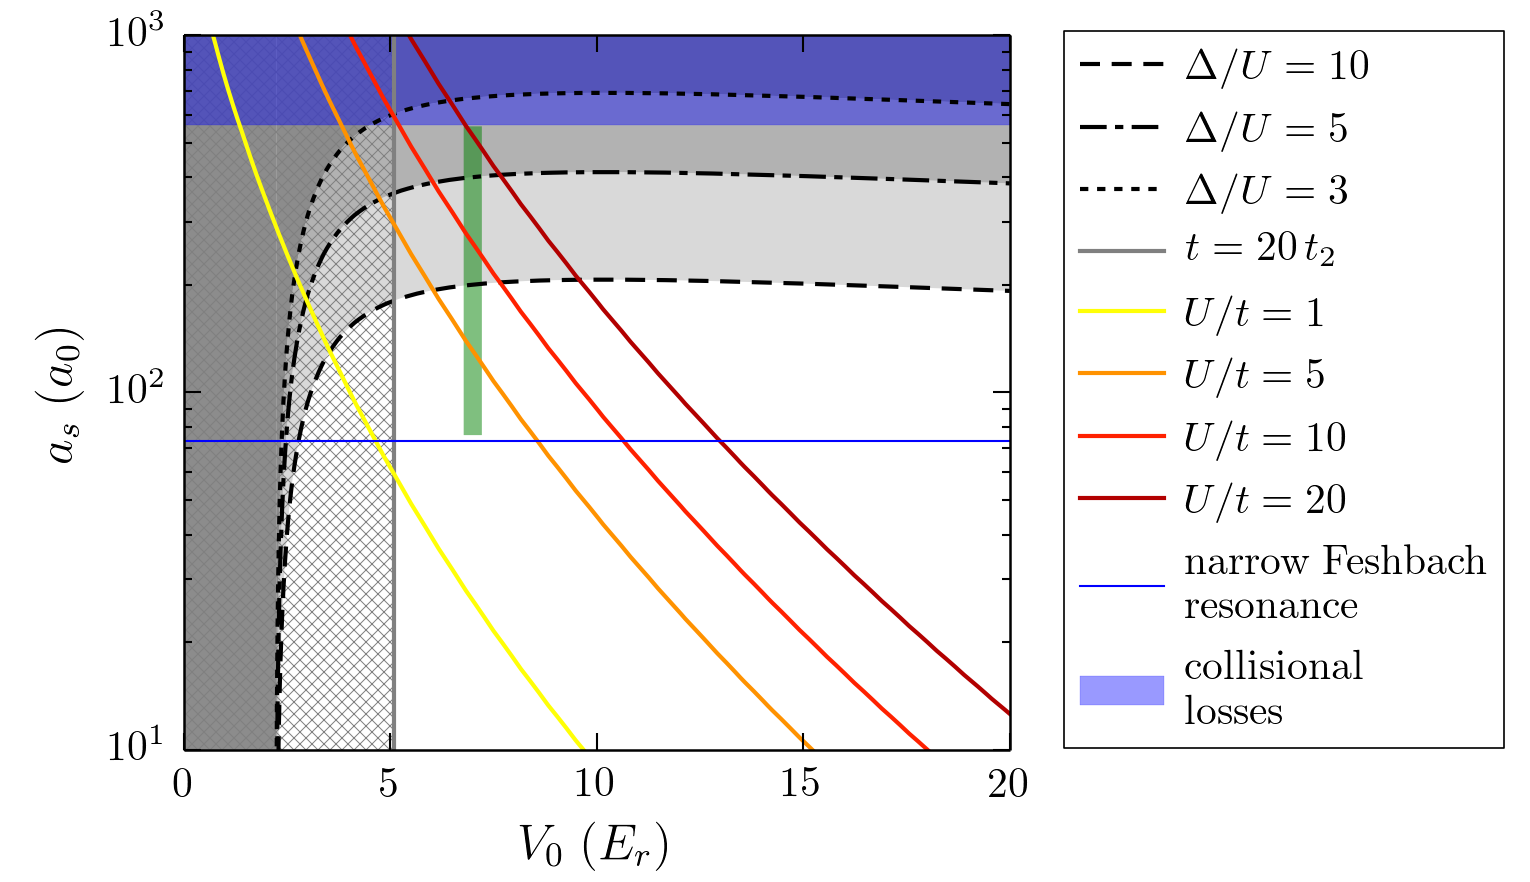
\includegraphics[width=0.9\textwidth]{../figures/BandStructure_figures/singleband.png}
\caption[Regimes of validity for the single band Hubbard Hamiltonian]{\small
Regimes of validity for the single band Hubbard Hamiltonian.   The dashed black
lines show curves at constant $\Delta/U$.  As $U$ approaches $\Delta$, higher
bands have to be taken into account to describe the system
accurately~\cite{Werner2005}.  The vertical gray line indicates the lattice
depth at which $t = 20t_{2}$, which delimits the region of validity of the
tight-binding approximation.  Yellow to brown hued lines indicated curves at
constant $U/t$.  The thin blue line indicates the background $s$-wave
scattering length in the vicinity of the narrow Feshbach resonance of
$^{6}Li$~\cite{Strecker2003,Zurn2013}.  The shaded blue area indicates the
range of scattering lengths over which we see significant collisional losses
and heating of the sample.   The shaded green area denotes the parameter regime
covered by the experiments carried out in this thesis.} 
\label{fig:hubbardvalid}
\end{figure}


 
%%%%%%%%%%%%%%%%%%%%%%%%%%%%%%%%%%%%%%%%%%%%%%%%%%%%%%%%%%%%%%%%%%%%%%%%%%%%%%%
%%%%%%%%%%%%%%%%%%%%%%%%%%%%%%%%%%%%%%%%%%%%%%%%%%%%%%%%%%%%%%%%%%%%%%%%%%%%%%%
%%%%  CHAPTER 3 
%%%%%%%%%%%%%%%%%%%%%%%%%%%%%%%%%%%%%%%%%%%%%%%%%%%%%%%%%%%%%%%%%%%%%%%%%%%%%%%
%%%%%%%%%%%%%%%%%%%%%%%%%%%%%%%%%%%%%%%%%%%%%%%%%%%%%%%%%%%%%%%%%%%%%%%%%%%%%%%
\chapter{The Hubbard model}
\label{chap:hubbardmodel}

In Chapter 2 we saw how ultracold atoms, under a large range of values for the
lattice depth and the $s$-wave scattering length are a nearly ideal realization
of the single band Hubbard model.   The Hubbard model, nevertheless, was not
originally formulated with these kind of systems in mind; it originated as an
overly simplified picture for the description of electrons in solids.   In this
chapter we start by providing a brief historical perspective of the Hubbard
model.  We then go on to introduce simplified treatments of the model which
will allow us to gain insight into its physics. We conclude by describing some
of the latest advances in numerical simulations. 

\section{A bit of history}

%The contents of this section are based on the book ``Out of the Crystal
%Maze''~\cite{hoddeson1992out}, which chronicles the origin and development of
%solid state physics from 1920 to 1960. 

% References: 
%
% Louis Neel Nobel Lecture
% Out of the Crystal Maze
% Magnetism in condensed matter  
% Hubbard's original paper. 

At the end of the 1920's, when the foundations of quantum mechanics were almost
all formally laid out, there were quite a few phenomena begging for a touch of
quantum mechanics to elucidate the physics behind them.  One of those problems
was ferromagnetism.    Ferromagnetism was first understood classically within
the Weiss picture of a molecular field,   in which a ferromagnet is treated as
a paramagnet under the influence of a fictitious magnetic field (the molecular
field), which is postulated to be proportional to the magnetization.  It was
Heisenberg in 1928~\cite{Heisenberg:1928:TFG} who realized that the exchange
interaction, as used by Heitler and London to explain the singlet and triplet
energy level splitting of the Helium atom, was responsible for the existence
and magnitude of Weiss's molecular field.   This motivated the Heisenberg model for ferromagnetism 
\begin{equation}
   H = -\sum_{ij} J_{ij} \bv{S}_{i} \cdot \bv{S}_{j} 
\end{equation} 
where $J_{ij}$ is the exchange constant between spins  that are localized at
sites  $i$  and $j$ in a crystal lattice.  Under the assumption that only
nearest neighboring spins affect each other, the Heisenberg model can account
for the Curie temperature of ferromagnets, with reasonable values of $J$ as an
input.  However, even though Heisenberg's theory of ferromagnetism had the
correct physical basis, a formal calculation of the exchange term, $J$, for a
large system of interacting electrons is too difficult to carry out.  

% Further work by
%Bloch, Slater, Bethe and others led to further understanding of the
%ferromagnetic state, such as the discovery of spin waves.  However, the problem
%remained a challenge, primarily due to the interactions between electrons.  


%Around the same time as Heisenberg developed his theory of ferromagnetism,  his
%Ph.D student Felix Bloch established the theory of energy bands (tight-binding
%model) to describe the behavior of conduction electrons in
%solids~\cite{Bloch1929lattice}.    
%At the time there was some dissatisfaction
%with the work of Heisenberg, because even though it had the correct physical
%basis, a formal calculation of the exchange term for a large system of
%interacting electrons proved too difficult to carry out.  With iron being a
%ferromagnetic metal, the role that the $s$ conduction electrons could be
%playing in its ferromagnetic properties (for instance the interaction of $d$
%electrons with $s$ electrons)  was an important question, which Bloch set out
%to answer using his band theory as a starting point.   Bloch realized that the
%exchange term could sometimes have a negative sign, which would not be
%consistent with ferromagnetism.  He came to the conclusion that, only for
%narrow energy bands (which favor wavefunctions that are more localized around
%the atoms), would the exchange interaction produce a ferromagnetic state.   Bloch was unable to 
%
% Pauli paramagnetism ( magnetism of the spins ) 
% Landau diagmagnetism ( magnetism of the free electrons being charged 
% particles and quantized Landau levels in B field)

%By the early 1930's, the band theory of solids, developed by Bloch during his
%PhD in 1928~\cite{Bloch1929lattice},  had become the foundation of solid state
%physics. In the following years, the interest in the field began to shift from
%general principles to computation of the properties of particular materials.
%Nevertheless, 

The problem of $d$ electrons in ferromagnetic metals  was still of much
interest in the early 1960's.    A lot of attention had been given in the
previous decade to the issue of considering the consequences of interactions
between electrons (correlations) in a free electron gas.  This was very
important for the description of electrons in conduction bands, but not
satisfactory when considering partially filled $d$ or $f$ bands, such as those
present in the transition and rare-earth metals.    In particular, the $d$
electrons of the transition metals  were of major interest at the time because
they are not as localized as $f$ electrons, but also not as ``free'' as
$s$-electrons in a conduction band.  

Hubbard realized, in the early 60's, that the problem of $d$-electrons could be
thought of as a problem of electrons in a conduction band, where the effects of
interactions between electrons (correlations) give rise to behavior more
consistent with an atomic picture of localized electrons. He then postulated a
model~\cite{Hubbard26111963}, now known as the Hubbard model,  as an extension
of the tight-binding model (the simplest model for an energy band) on which the
effects of correlations are simplified at maximum without removing them
altogether.   The hope was to see the behavior of electrons as localized
moments, i.e. ferromagnetism or an insulating state, emerge solely as a
consequence of electron correlations in a conduction band. 

To simplify the role of correlations, Hubbard neglected all of the terms due to
interactions, except the one where two electrons are on the same site.  As we
saw in Chapter~2, this approximation is easy to express in the second quantized
formalism using Wannier states as a single particle basis.  The on-site
interaction term for the Coulomb energy between two electrons is then:
\begin{equation}
U =  \int 
      w^{*}( \bv{x} - \bv{R}_{i} )
      w( \bv{x} - \bv{R}_{k} )
 \left( \frac{ e^{2} }{ | \bv{x} - \bv{x}' | } \right) 
      w^{*}( \bv{x}' - \bv{R}_{j} )
      w( \bv{x}' - \bv{R}_{l} )
 \ \mathrm{d}\bv{x}\mathrm{d}\bv{x}'
\end{equation}
where $w$ are the Wannier states, introduced in Chapter~2, and $\bv{R}_{i} =
\bv{R}_{j} = \bv{R}_{k} = \bv{R}_{l}$.  In the same year as Hubbard,
Gutzwiller~\cite{PhysRevLett.10.159} and Kanamori~\cite{Kanamori01091963},
independently formulated essentially the same model for $d$ electrons. 

Another thing to point out about the Hubbard model is that even though it was
conceived with the problem of $d$-electrons in mind, the band considered in the
model is an $s$-band. In a $d$-band there are 10 different levels that an
electron can occupy, however in an $s$-band there are only two, spin up and
spin down.  Hubbard himself commented on this point and said: ``one may
nevertheless hope to obtain some results of general
application''~\cite{Hubbard26111963},.  

%In 1936 Louis N\'{e}el noted that, since the exchange energy originates from
%short range overlap between wavefunctions, then it would be possible for it to
%give rise to an antiferromagnetic state.   An antiferromagnetic state can form
%in a bipartite lattice,  a lattice that can be subdivided into two sublattices
%such that for any given site all of its neighbors belong to the other
%sublattice.   For a system with a negative value of the exchange integral then
%the antiferroma 

\section{Hubbard model for a single lattice site, $t=0$}

%For a more complete introduction to the Hubbard model refer to
%Ref.~\cite{Scalettar:hubbard7}. 

In the Hubbard model, the limit of no interactions,  $U=0$, takes us simply
back to the tight-binding model.  In this case the properties of the system can
be well understood in terms of a single particle picture, where electrons
occupy the single particle energy levels of the Hamiltonian according to the
Fermi-Dirac distribution.  The dispersion relation of the tight-binding model
determines the density of states, and the thermodynamics at low temperature can
be obtained from the value of the Fermi energy and the temperature by making
use of Sommerfeld's approach for approximating Fermi-Dirac
integrals~\cite{ashcroft1976solid}.

On the other hand, the limit of no tunneling~\cite{Scalettar:hubbard7}, $t=0$,
will allow us to gain some insight into the thermodynamics of the Hubbard
model.  In this case the lattice sites can be considered to be completely
independent of each other, and the partition function of the total system is
simply a product of the partition function for a system with a single lattice
site.

We recall the Hubbard Hamiltonian:
\begin{equation}
  H =  
-t \sum_{ \langle ij \rangle, \sigma   } 
          a_{i\sigma}^{\dagger}a_{j\sigma} 
         + U\sum_{i} n_{i\spup} n_{i\spdn}  
   - \mu \sum_{i}  ( n_{i\spup} + n_{i\spdn} ) 
\end{equation}
where $\mu$ is the chemical potential, and the term $- \mu \sum_{i}  (
n_{i\spup} + n_{i\spdn} ) $ is included to work in the grand
canonical ensemble, where the particle number is allowed to vary. 

The grand canonical partition function is given by
\begin{equation} 
 Z = \text{Tr} e^{-\beta H}  =  z^{N} 
\end{equation} 
where $z$ is the partition function for an individual site given by
\begin{equation}
  z = 1 + 2e^{\beta\mu} + e^{2\beta\mu - \beta U} 
\end{equation}
With the partition function in hand we can obtain the thermodynamic quantities
as derivatives of the grand canonical potential, $\Omega = - \ln Z /
\beta $.  We have for the density, double occupancy, and entropy per lattice
site:
\begin{equation}
  n  = -\frac{1}{N}\frac{\partial \Omega}{ \partial \mu } ~~~~~~~~~
  d  = \frac{1}{N}\frac{\partial \Omega}{ \partial U }  ~~~~~~~~~
  s  = -\frac{1}{N}\frac{\partial \Omega}{ \partial T} 
\end{equation}

For example, the explicit expression for the density can be derived:
\begin{equation}
  n  = 2\frac{ e^{\beta \mu} + e^{2\beta\mu - \beta U} }
          { 1 + 2e^{\beta \mu} + e^{2\beta\mu-\beta U } } 
\end{equation}
An important physical quantity in the Hubbard model is the local moment,
defined as 
\begin{equation}
  \langle m ^{2} \rangle = \langle ( n_{\spup} - n_{\spdn} )^{2} \rangle  = n - 2d 
\end{equation} 
If there is no probability of having doubly occupied sites, $d=0$ and the local
moment simply becomes equal to the density $n$.   From the grand potential we
obtain the expression
\begin{equation} 
  \langle m ^{2} \rangle =  2\frac{ e^{\beta \mu}  }
          { 1 + 2e^{\beta \mu} + e^{2\beta\mu-\beta U } } 
\end{equation}
 
In Fig.~\ref{fig:0t_occupation} we show plots of the density and the local
moment versus chemical potential for various temperatures.  As we mentioned
above, the Hubbard model describes an $s$-band with a maximum capacity of two
electrons per lattice site.   When the average number of particles per site in
the Hubbard model  is $n=1$, the system is said to be at half-filling.
Figure~\ref{fig:0t_occupation} shows us that there is a plateau in the density
as a function of chemical potential which occurs at half-filling for
sufficiently low temperatures.   This plateau is an indication of the Mott
insulating gap, it can be interpreted as a discontinuous jump in the energy
necessary to add an extra particle to the system.   At the same time we see
that the local moment goes to 1, equal to the density at half filling, which
tells us that in the Mott insulating plateau the probability of finding doubly
occupied sites goes to zero, as well as the fluctuations in the number of
particles per site 
\begin{figure}
\centering
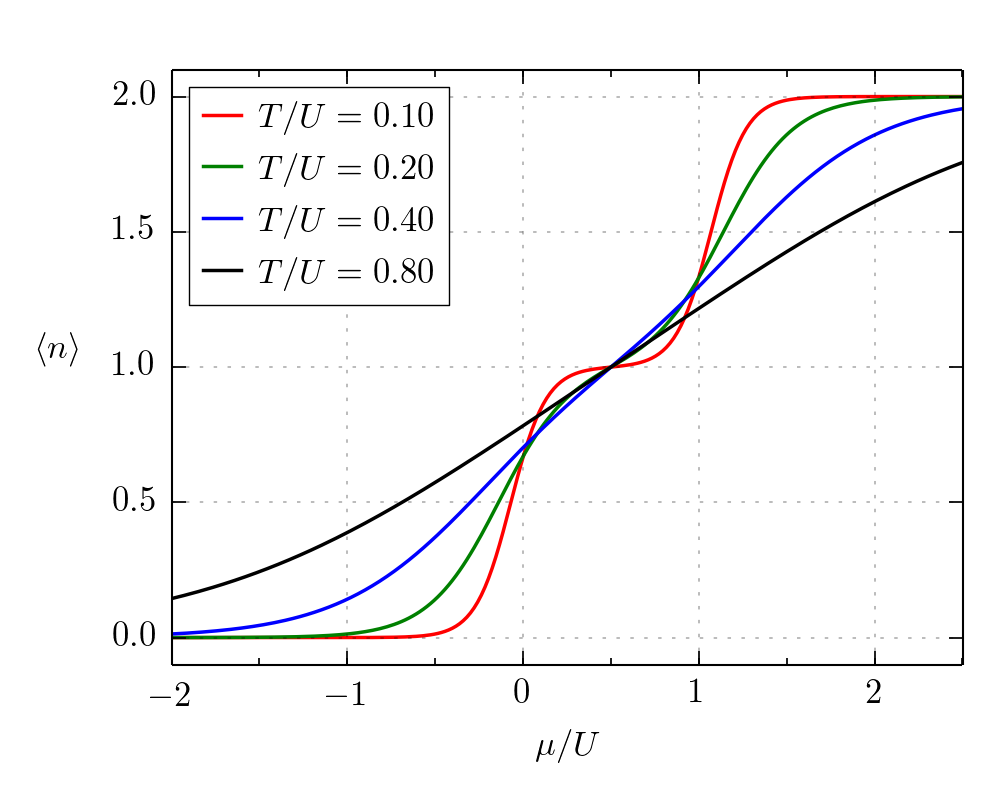
\includegraphics[width=0.48\textwidth]{../figures/hubbard/hubbard_0t_occupation.png}
~
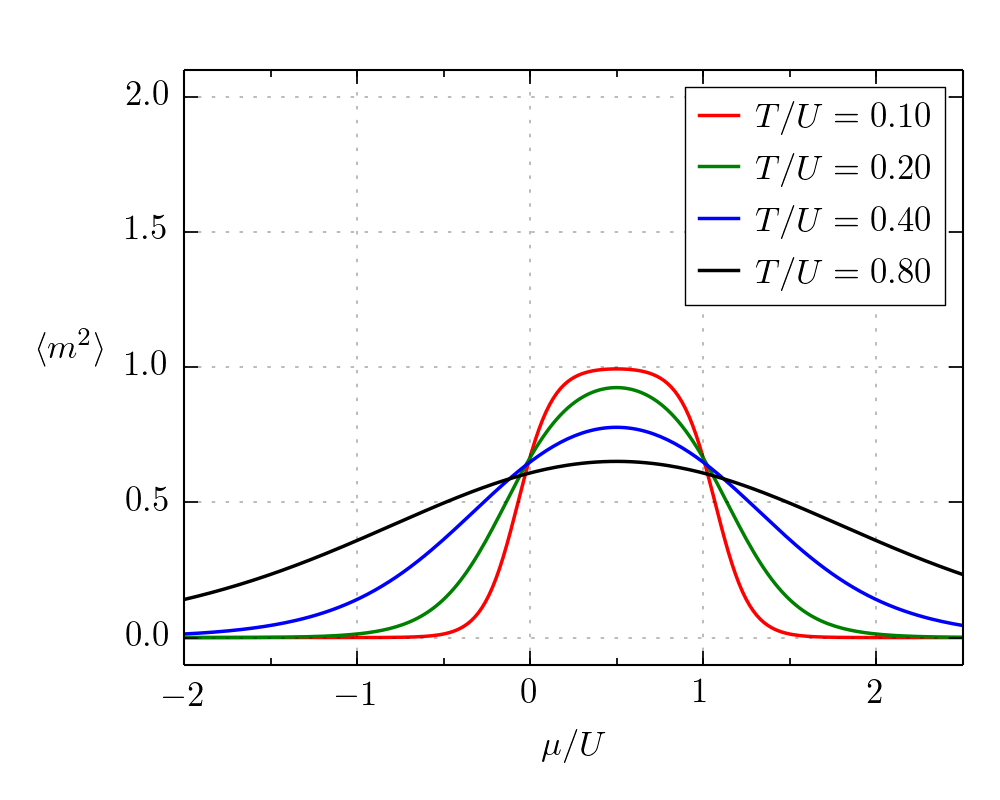
\includegraphics[width=0.48\textwidth]{../figures/hubbard/hubbard_0t_moments.png}
\caption[Density and local moment in the Hubbard model at $t=0$]{\small Density
and local moment versus chemical potential in the Hubbard model for $t=0$.  In
this limit the Hubbard model represents a collection of uncorrelated lattice
sites.  For a temperature, $T$, significantly lower than the on-site
interaction, $U$,  the density shows a plateau as a function of chemical
potential, representative of the Mott insulating gap. At the same time the
local moment goes to 1, indicating the absence of doubly occupied sites, and
the suppression of fluctuations on the number of atoms per site, two indicators
of an insulating state.  } 
\label{fig:0t_occupation}
\end{figure}

In the previous paragraph we suggested that the plateau in $n$ vs. $\mu$ is
indicative of an energy gap.  In more formal terms, to establish the presence
of a gap in the spectrum of a many-body system, one should calculate the
pseudo-particle density of states (also known as the spectral function).  This
was done by Hubbard on the third of the series of papers that followed his
introduction of the Hubbard model~\cite{Hubbard1964}, and he showed that his
model predicted the  existence of the Mott-Hubbard insulating gap.  In 1949,
Mott had suggested that the Coulomb interaction was responsible for the
insulating properties of nickel monoxide (NiO), a material with a partially
filled band that should be a conductor according to conventional band
theory~\cite{Mott1949}.  The treatment by Hubbard was the first formal
treatment of the Mott metal-insulator transition~\cite{RevModPhys.40.677} and
the first big success of the Hubbard model.


\section{Particle-hole symmetry} 

The reader may have noticed, by looking at Fig.~\ref{fig:0t_occupation}, that
all of the plotted curves have a symmetry about $\mu=U/2$.    All of the the
thermodynamic properties of the Hubbard model exhibit this symmetry, a
consequence of the particle-hole symmetry of the Hamiltonian,  and one only
needs to obtain them for densities $0\leq n \leq 1$, as they can be inferred
for $1\leq n \leq 2$ by reflection about $\mu=U/2$.  In some theoretical
treatments it is desirable to have the reflection point be independent of $U$,
so a shift is introduced in the chemical potential $\mu' = \mu-U/2$ which
results in the ``particle-hole symmetric'' form of the Hubbard Hamiltonian:
\begin{equation}
  H' =  
-t \sum_{ \langle ij \rangle, \sigma   } 
          a_{i\sigma}^{\dagger}a_{j\sigma} 
         + U\sum_{i} \left( n_{i\spup} -\frac{1}{2}\right) 
                     \left( n_{i\spdn} -\frac{1}{2}\right) 
   - \mu' \sum_{i}  ( n_{i\spup} + n_{i\spdn} ) 
\end{equation}
This form produces the same physical results as the non-shifted one. 
 

\section{Exact diagonalization} 

The treatment of the single-site limit of the Hubbard model was very simple and
we showed how to obtain an expression for the grand potential, from which all of
the thermodynamic properties can be obtained.  From this simple treatment we
saw how the Mott insulating gap opens up at low temperatures, and a Mott
insulator, with exactly one particle per lattice site, can exist at
half-filling.   At even lower temperatures it is well known that the localized
moments of the Mott insulator order themselves into an AFM ordered state. 

In what follows we will obtain the exact solution for the ground state of
models with 2 sites and 4 sites.  These solutions are going to motivate the
antiferromagnetic character of the ground state of the Hubbard model, and give
us a glimpse of the connection between the Hubbard model and high-$T_{c}$
superconductivity. 

\subsubsection { Exact diagonalization for 2 sites } 

The full Hilbert space for a two-site model has dimension 16.  To do an exact
diagonalization we will restrict to a sector at half-filling with a balanced
spin-mixture (equal number of up and down spins).  The basis states are:
\begin{align}
  |\ndbl, \nvac \rangle  & =  
      a_{1\spup}^{\dagger} a_{1\spdn}^{\dagger} |\nvac\rangle \\  
  |\nspdn, \nspup \rangle & =    
      a_{1\spdn}^{\dagger} a_{2\spup}^{\dagger} |\nvac\rangle \\  
  |\nspup, \nspdn \rangle & =   
      a_{1\spup}^{\dagger} a_{2\spdn}^{\dagger} |\nvac\rangle \\  
  | \nvac, \ndbl \rangle & =  
      a_{2\spup}^{\dagger} a_{2\spdn}^{\dagger} |\nvac\rangle \\  
\end{align}
Notice that we have chosen the ordering convention for fermion creation
operators in which lower site indices are leftmost and spin up is to the left
of spin down.   Calculating the matrix elements of the Hubbard Hamiltonian in
this basis is an exercise in tracking minus signs when commuting fermion
creation and annihilation operators.   We have automated that procedure by
writing a python program which is available online~\cite{PedroMDuarte:11558}.

The resulting matrix for the Hamiltonian is 
\begin{equation}
H =   
\left(
\begin{array}{cccc}
 U & 0 & -t & -t \\
 0 & U & -t & -t \\
 -t & -t & 0 & 0 \\
 -t & -t & 0 & 0 \\
\end{array}
\right)  
\end{equation}
which can be analytically diagonalized to obtain the eigenvalues
\begin{equation}
\begin{array}{c}
 \frac{1}{2} \left(U-\sqrt{16 t^2+U^2}\right) \\
 0 \\
 U \\
 \frac{1}{2} \left(U+\sqrt{16 t^2+U^2}\right) \\
\end{array}
\end{equation}
For large $U/t$ the energy of the ground state goes to $\approx -4 t^{2}/U$,
which is the value of the AFM exchange energy.  In Fig.~\ref{fig:exact_2site}
we show plots of the energy eigenvalues as a function of $U/t$ and also show
the composition of the energy eigenstates in terms of our basis states.  
\begin{figure}
\centering
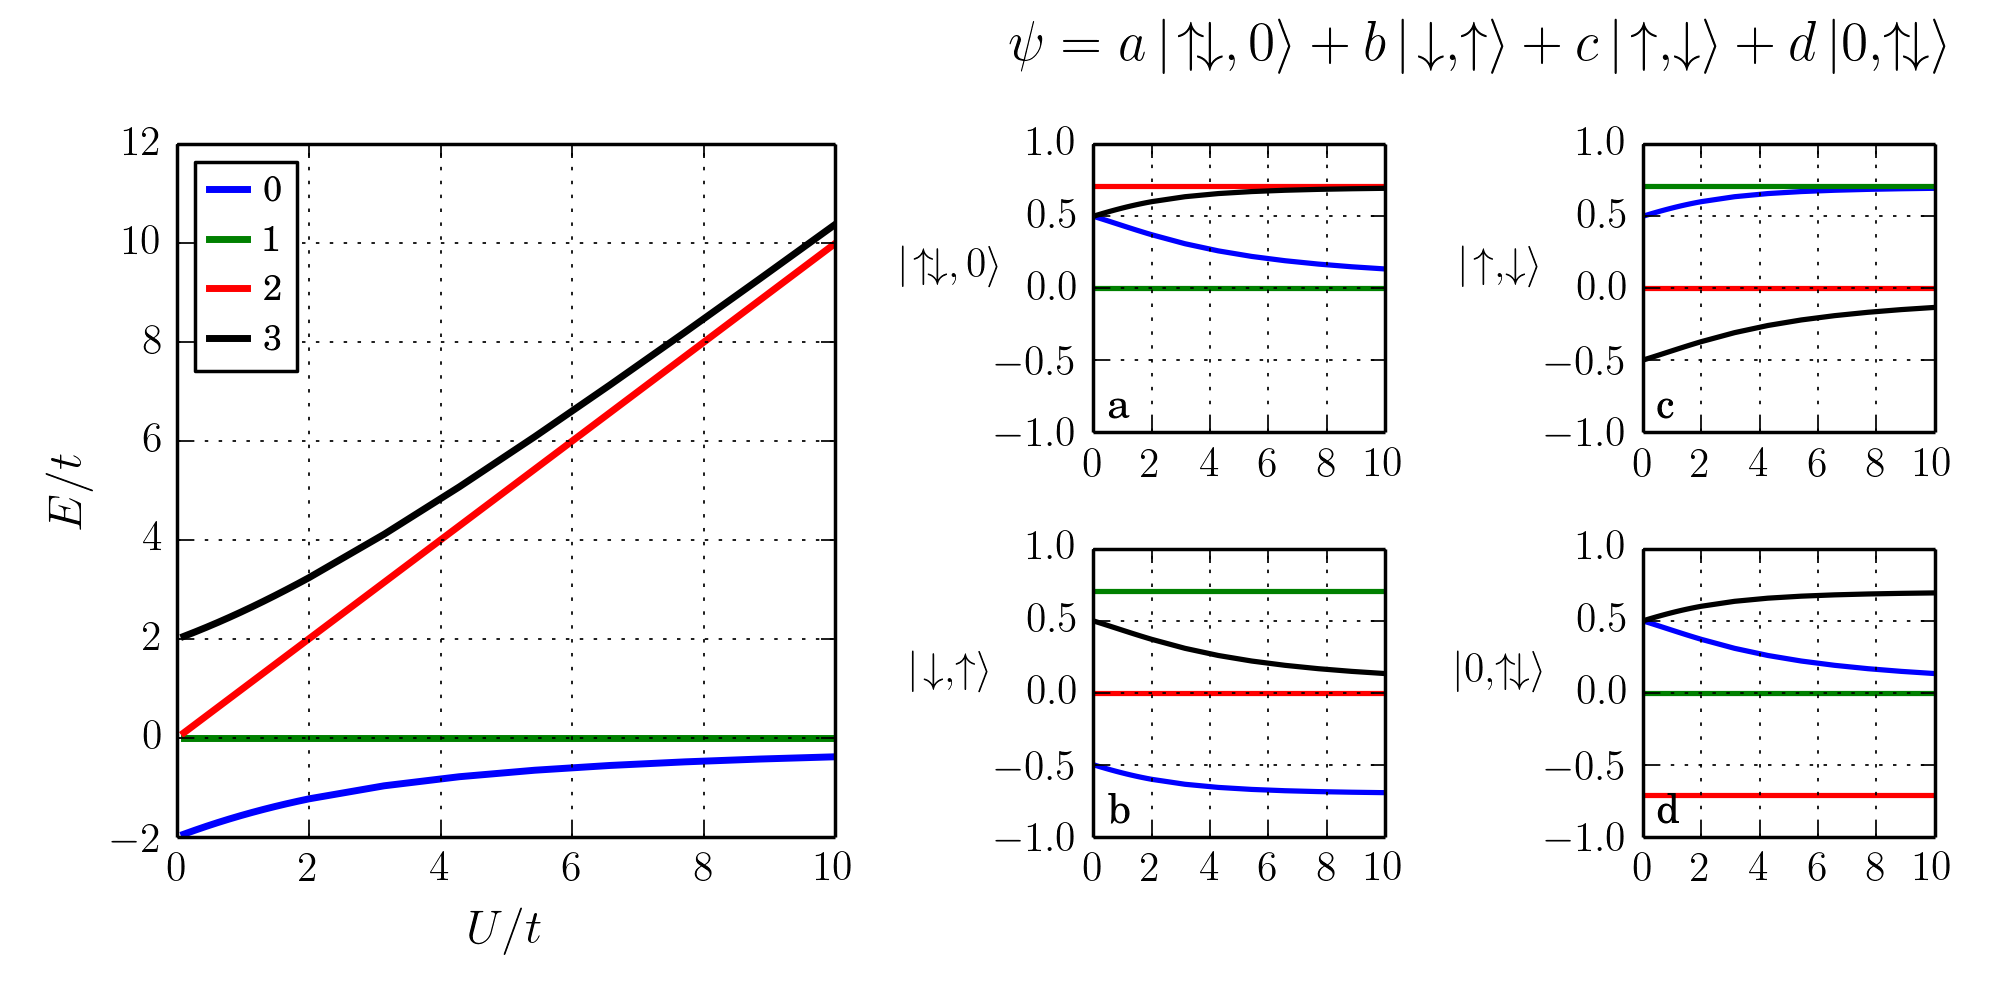
\includegraphics[width=0.7\textwidth]{../figures/hubbard/Ut_eigenvalues_2site.png}
\caption[Exact diagonalization results for two lattice sites.]{\small Energy
eigenvalues and eigenstates for a two lattice site system.  The coefficients
$a,b,c,d$, which define the energy eigenstates are shown in the four panels at
the right.  We see that the ground state has an antiferromagnetic character. } 
\label{fig:exact_2site}
\end{figure}
In the two-site system, we can see the opening of the Mott-Hubbard gap in the
spectrum as $U/t$ is increased, in agreement with the single site treatment.
We can now also see the antiferromagnetic character of the ground state.  In
the limit of large $U/t$, the ground state is given by 
\begin{equation}
    \frac{1}{\sqrt{2}} | \nspup, \nspdn\rangle  
  - \frac{1}{\sqrt{2}} | \nspdn, \nspup\rangle 
\end{equation} 


\subsubsection { Exact diagonalization for 4 sites } 

In the case of four lattice sites (a $2\times$2 plaquette), the basis set in the
half-filling spin-balanced sector grows to contain 36 states.   The Hamiltonian
matrix is a 36$\times$36 matrix, which can be readily diagonalized numerically.
% TO SEE THE MATRIX FOR THE 2X2 PROBLEM UNCOMMENT BELOW
%\begin{equation} \tiny \arraycolsep=1.0pt\def\arraystretch{0.6} \left(
%\begin{array}{cccccccccccccccccccccccccccccccccccc} 2 U & 0 & -t & 0 & t & 0 &
%0 & 0 & 0 & -t & 0 & 0 & 0 & 0 & 0 & 0 & 0 & 0 & t & 0 & 0 & 0 & 0 & 0 & 0 & 0
%& 0 & 0 & 0 & 0 & 0 & 0 & 0 & 0 & 0 & 0 \\ 0 & U & -t & 0 & 0 & 0 & 0 & t & 0
%& t & 0 & 0 & 0 & 0 & 0 & 0 & 0 & 0 & 0 & 0 & -t & 0 & 0 & 0 & 0 & 0 & 0 & 0 &
%0 & 0 & 0 & 0 & 0 & 0 & 0 & 0 \\ -t & -t & U & 0 & 0 & 0 & 0 & 0 & -t & 0 & t
%& t & 0 & 0 & 0 & 0 & 0 & 0 & 0 & 0 & 0 & -t & 0 & 0 & 0 & 0 & 0 & 0 & 0 & 0 &
%0 & 0 & 0 & 0 & 0 & 0 \\ 0 & 0 & 0 & U & -t & 0 & t & 0 & 0 & 0 & 0 & 0 & -t &
%0 & 0 & 0 & 0 & 0 & t & 0 & 0 & 0 & 0 & 0 & 0 & 0 & 0 & 0 & 0 & 0 & 0 & 0 & 0
%& 0 & 0 & 0 \\ t & 0 & 0 & -t & U & 0 & 0 & 0 & t & 0 & 0 & 0 & 0 & 0 & t & 0
%& 0 & 0 & 0 & t & 0 & 0 & 0 & 0 & -t & 0 & 0 & 0 & 0 & 0 & 0 & 0 & 0 & 0 & 0 &
%0 \\ 0 & 0 & 0 & 0 & 0 & 2 U & -t & t & 0 & 0 & 0 & 0 & -t & 0 & 0 & 0 & 0 & 0
%& 0 & 0 & t & 0 & 0 & 0 & 0 & 0 & 0 & 0 & 0 & 0 & 0 & 0 & 0 & 0 & 0 & 0 \\ 0 &
%0 & 0 & t & 0 & -t & U & 0 & -t & 0 & 0 & 0 & 0 & -t & 0 & 0 & t & 0 & 0 & 0 &
%0 & t & 0 & 0 & 0 & 0 & 0 & 0 & 0 & 0 & 0 & 0 & 0 & 0 & 0 & 0 \\ 0 & t & 0 & 0
%& 0 & t & 0 & U & t & 0 & 0 & 0 & 0 & 0 & -t & 0 & 0 & 0 & 0 & 0 & 0 & 0 & t &
%0 & 0 & t & 0 & 0 & 0 & 0 & 0 & 0 & 0 & 0 & 0 & 0 \\ 0 & 0 & -t & 0 & t & 0 &
%-t & t & 2 U & 0 & 0 & 0 & 0 & 0 & 0 & -t & 0 & -t & 0 & 0 & 0 & 0 & 0 & t & 0
%& 0 & t & 0 & 0 & 0 & 0 & 0 & 0 & 0 & 0 & 0 \\ -t & t & 0 & 0 & 0 & 0 & 0 & 0
%& 0 & U & -t & t & 0 & 0 & -t & 0 & 0 & 0 & 0 & 0 & 0 & 0 & 0 & 0 & 0 & 0 & 0
%& -t & 0 & 0 & 0 & 0 & 0 & 0 & 0 & 0 \\ 0 & 0 & t & 0 & 0 & 0 & 0 & 0 & 0 & -t
%& U & 0 & 0 & 0 & 0 & t & 0 & 0 & 0 & 0 & 0 & 0 & 0 & 0 & 0 & 0 & 0 & 0 & -t &
%0 & 0 & 0 & 0 & 0 & 0 & 0 \\ 0 & 0 & t & 0 & 0 & 0 & 0 & 0 & 0 & t & 0 & 0 & 0
%& 0 & 0 & 0 & 0 & t & 0 & 0 & 0 & 0 & 0 & 0 & 0 & 0 & 0 & 0 & 0 & 0 & 0 & t &
%0 & 0 & 0 & 0 \\ 0 & 0 & 0 & -t & 0 & -t & 0 & 0 & 0 & 0 & 0 & 0 & U & -t & t
%& 0 & -t & 0 & 0 & 0 & 0 & 0 & 0 & 0 & 0 & 0 & 0 & -t & 0 & 0 & 0 & 0 & 0 & 0
%& 0 & 0 \\ 0 & 0 & 0 & 0 & 0 & 0 & -t & 0 & 0 & 0 & 0 & 0 & -t & 0 & 0 & -t &
%0 & 0 & 0 & 0 & 0 & 0 & 0 & 0 & 0 & 0 & 0 & 0 & -t & 0 & 0 & 0 & 0 & 0 & 0 & 0
%\\ 0 & 0 & 0 & 0 & t & 0 & 0 & -t & 0 & -t & 0 & 0 & t & 0 & 0 & t & 0 & -t &
%0 & 0 & 0 & 0 & 0 & 0 & 0 & 0 & 0 & 0 & 0 & -t & 0 & 0 & 0 & t & 0 & 0 \\ 0 &
%0 & 0 & 0 & 0 & 0 & 0 & 0 & -t & 0 & t & 0 & 0 & -t & t & U & 0 & 0 & 0 & 0 &
%0 & 0 & 0 & 0 & 0 & 0 & 0 & 0 & 0 & 0 & -t & 0 & 0 & 0 & t & 0 \\ 0 & 0 & 0 &
%0 & 0 & 0 & t & 0 & 0 & 0 & 0 & 0 & -t & 0 & 0 & 0 & U & t & 0 & 0 & 0 & 0 & 0
%& 0 & 0 & 0 & 0 & 0 & 0 & 0 & 0 & -t & 0 & 0 & 0 & 0 \\ 0 & 0 & 0 & 0 & 0 & 0
%& 0 & 0 & -t & 0 & 0 & t & 0 & 0 & -t & 0 & t & U & 0 & 0 & 0 & 0 & 0 & 0 & 0
%& 0 & 0 & 0 & 0 & 0 & 0 & 0 & -t & 0 & 0 & -t \\ t & 0 & 0 & t & 0 & 0 & 0 & 0
%& 0 & 0 & 0 & 0 & 0 & 0 & 0 & 0 & 0 & 0 & U & -t & 0 & t & 0 & 0 & -t & 0 & 0
%& t & 0 & 0 & 0 & 0 & 0 & 0 & 0 & 0 \\ 0 & 0 & 0 & 0 & t & 0 & 0 & 0 & 0 & 0 &
%0 & 0 & 0 & 0 & 0 & 0 & 0 & 0 & -t & U & 0 & 0 & 0 & t & 0 & 0 & 0 & 0 & 0 &
%-t & 0 & 0 & 0 & 0 & 0 & 0 \\ 0 & -t & 0 & 0 & 0 & t & 0 & 0 & 0 & 0 & 0 & 0 &
%0 & 0 & 0 & 0 & 0 & 0 & 0 & 0 & U & -t & t & 0 & 0 & -t & 0 & t & 0 & 0 & 0 &
%0 & 0 & 0 & 0 & 0 \\ 0 & 0 & -t & 0 & 0 & 0 & t & 0 & 0 & 0 & 0 & 0 & 0 & 0 &
%0 & 0 & 0 & 0 & t & 0 & -t & 0 & 0 & -t & 0 & 0 & t & 0 & t & 0 & 0 & -t & 0 &
%0 & 0 & 0 \\ 0 & 0 & 0 & 0 & 0 & 0 & 0 & t & 0 & 0 & 0 & 0 & 0 & 0 & 0 & 0 & 0
%& 0 & 0 & 0 & t & 0 & 0 & t & 0 & 0 & 0 & 0 & 0 & t & 0 & 0 & 0 & 0 & 0 & 0 \\
%0 & 0 & 0 & 0 & 0 & 0 & 0 & 0 & t & 0 & 0 & 0 & 0 & 0 & 0 & 0 & 0 & 0 & 0 & t
%& 0 & -t & t & U & 0 & 0 & 0 & 0 & 0 & 0 & t & 0 & t & 0 & 0 & 0 \\ 0 & 0 & 0
%& 0 & -t & 0 & 0 & 0 & 0 & 0 & 0 & 0 & 0 & 0 & 0 & 0 & 0 & 0 & -t & 0 & 0 & 0
%& 0 & 0 & 0 & 0 & -t & 0 & 0 & 0 & 0 & 0 & 0 & -t & 0 & 0 \\ 0 & 0 & 0 & 0 & 0
%& 0 & 0 & t & 0 & 0 & 0 & 0 & 0 & 0 & 0 & 0 & 0 & 0 & 0 & 0 & -t & 0 & 0 & 0 &
%0 & U & t & 0 & 0 & 0 & 0 & 0 & 0 & -t & 0 & 0 \\ 0 & 0 & 0 & 0 & 0 & 0 & 0 &
%0 & t & 0 & 0 & 0 & 0 & 0 & 0 & 0 & 0 & 0 & 0 & 0 & 0 & t & 0 & 0 & -t & t & U
%& 0 & 0 & 0 & 0 & 0 & 0 & 0 & -t & t \\ 0 & 0 & 0 & 0 & 0 & 0 & 0 & 0 & 0 & -t
%& 0 & 0 & -t & 0 & 0 & 0 & 0 & 0 & t & 0 & t & 0 & 0 & 0 & 0 & 0 & 0 & 2 U &
%-t & t & 0 & -t & 0 & t & 0 & 0 \\ 0 & 0 & 0 & 0 & 0 & 0 & 0 & 0 & 0 & 0 & -t
%& 0 & 0 & -t & 0 & 0 & 0 & 0 & 0 & 0 & 0 & t & 0 & 0 & 0 & 0 & 0 & -t & U & 0
%& -t & 0 & 0 & 0 & -t & 0 \\ 0 & 0 & 0 & 0 & 0 & 0 & 0 & 0 & 0 & 0 & 0 & 0 & 0
%& 0 & -t & 0 & 0 & 0 & 0 & -t & 0 & 0 & t & 0 & 0 & 0 & 0 & t & 0 & U & t & 0
%& -t & 0 & 0 & 0 \\ 0 & 0 & 0 & 0 & 0 & 0 & 0 & 0 & 0 & 0 & 0 & 0 & 0 & 0 & 0
%& -t & 0 & 0 & 0 & 0 & 0 & 0 & 0 & t & 0 & 0 & 0 & 0 & -t & t & 2 U & 0 & 0 &
%0 & 0 & 0 \\ 0 & 0 & 0 & 0 & 0 & 0 & 0 & 0 & 0 & 0 & 0 & t & 0 & 0 & 0 & 0 &
%-t & 0 & 0 & 0 & 0 & -t & 0 & 0 & 0 & 0 & 0 & -t & 0 & 0 & 0 & U & t & 0 & 0 &
%-t \\ 0 & 0 & 0 & 0 & 0 & 0 & 0 & 0 & 0 & 0 & 0 & 0 & 0 & 0 & 0 & 0 & 0 & -t &
%0 & 0 & 0 & 0 & 0 & t & 0 & 0 & 0 & 0 & 0 & -t & 0 & t & U & 0 & 0 & 0 \\ 0 &
%0 & 0 & 0 & 0 & 0 & 0 & 0 & 0 & 0 & 0 & 0 & 0 & 0 & t & 0 & 0 & 0 & 0 & 0 & 0
%& 0 & 0 & 0 & -t & -t & 0 & t & 0 & 0 & 0 & 0 & 0 & U & t & t \\ 0 & 0 & 0 & 0
%& 0 & 0 & 0 & 0 & 0 & 0 & 0 & 0 & 0 & 0 & 0 & t & 0 & 0 & 0 & 0 & 0 & 0 & 0 &
%0 & 0 & 0 & -t & 0 & -t & 0 & 0 & 0 & 0 & t & U & 0 \\ 0 & 0 & 0 & 0 & 0 & 0 &
%0 & 0 & 0 & 0 & 0 & 0 & 0 & 0 & 0 & 0 & 0 & -t & 0 & 0 & 0 & 0 & 0 & 0 & 0 & 0
%& t & 0 & 0 & 0 & 0 & -t & 0 & t & 0 & 2 U \\ \end{array} \right)
%\end{equation}
The results for the eigenvalues and the coefficients of three of the
eigenvectors are shown in Fig.~\ref{fig:exact_4site}.
\begin{figure}
\centering
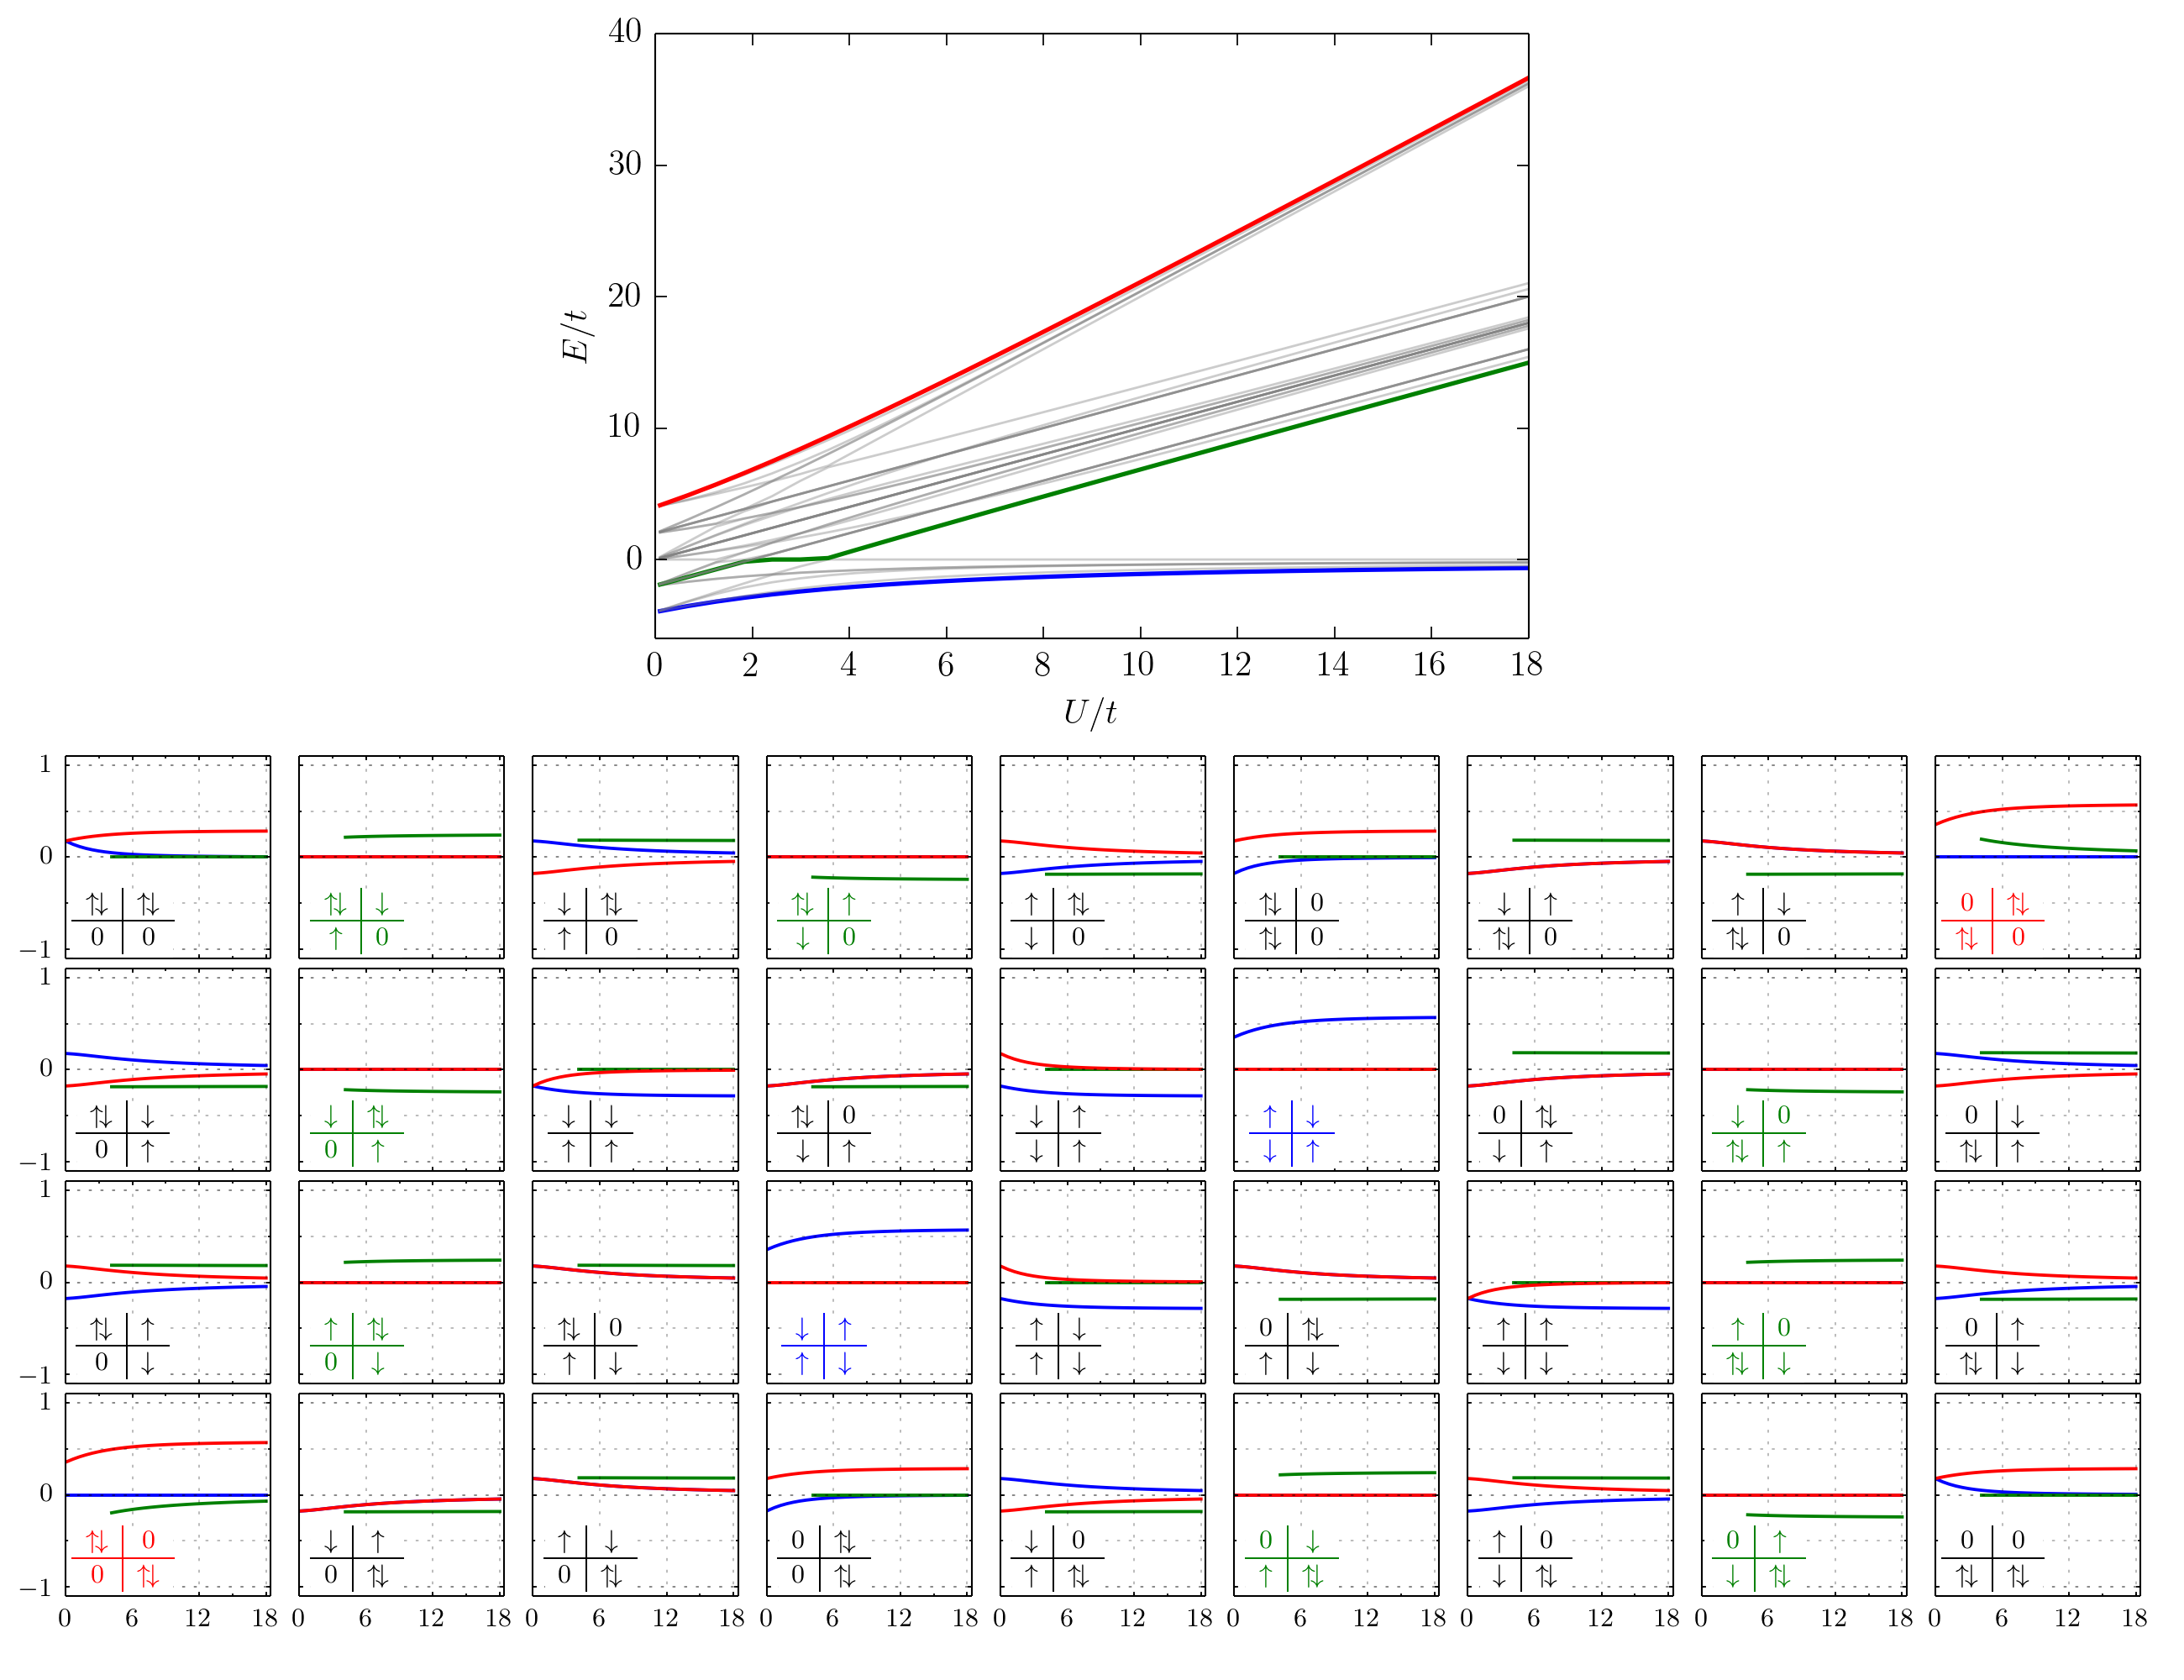
\includegraphics[width=1.0\textwidth]{../figures/hubbard/Ut_eigenvalues_4site.png}
\caption[Exact diagonalization results for a 4-site plaquette.]{\small Energy
eigenvalues and eigenstates for a 4-site plaquette.  In the top panel we show
the energy eigenvalues for all of the 36 different eigenstates.  We highlight
the ground state (blue),  the first state above the Mott-Hubbard gap (green)
and the highest energy state (red).  In the lower panels we show the
projections of each of the three highlighted states onto the basis states.
Each panel corresponds to a basis state as indicated by the diagram on the
lower left corner of the panels.  We have colored the state labels indicating
which states have the largest contribution to the eigenstates.    } 
\label{fig:exact_4site} 
\end{figure}

In the 4-site plaquette,  the largest contribution to the ground state comes
from states 
\begin{equation}
\arraycolsep=1.0pt\def\arraystretch{0.6}
  \left|
  \scalebox{0.75}{$ 
  \begin{array}{c|c}
    \nspdn & \nspup \\ \hline
    \nspup & \nspdn \\ \end{array}$ } \right\rangle =  
   a_{1\spdn}^{\dagger} a_{2\spup}^{\dagger} 
   a_{3\spup}^{\dagger} a_{4\spdn}^{\dagger} |\nvac\rangle
  ~~~~~~~~~~\text{and}~~~~~~~~~~
  \left|
  \scalebox{0.75}{$ 
  \begin{array}{c|c}
    \nspup & \nspdn \\ \hline
    \nspdn & \nspup \\ \end{array}$ } \right\rangle = 
   a_{1\spup}^{\dagger} a_{2\spdn}^{\dagger} 
   a_{3\spdn}^{\dagger} a_{4\spup}^{\dagger} |\nvac\rangle
\end{equation} 
where we have used the numbering convention
\scalebox{0.5}{\arraycolsep=1.0pt\def\arraystretch{0.7}$\begin{array}{c|c}
\makebox[1em][c]{$1$} &\makebox[1em][c]{$2$} \\ \hline \makebox[1em][c]{$3$}
&\makebox[1em][c]{$4$} \\ \end{array}$} to label the lattice sites.

There is something very important to notice in this case, though.  Going back
to the 2$\times$1 lattice we saw there was a minus sign between the two
antiferromagnetic configurations.  In this case, if we examine the panels in
Fig.~\ref{fig:exact_4site} we notice that the ground state has the largest
contributions from the antiferromagnetic configurations,  and that both
configurations show up with the same sign: 
\begin{equation} 
| \phi_{a} \rangle = 
   a_{1\spdn}^{\dagger} a_{2\spup}^{\dagger} 
   a_{3\spup}^{\dagger} a_{4\spdn}^{\dagger} |\nvac\rangle 
  ~~~~~~~~ 
|  \phi_{b} \rangle = 
   a_{1\spup}^{\dagger} a_{2\spdn}^{\dagger} 
   a_{3\spdn}^{\dagger} a_{4\spup}^{\dagger} |\nvac\rangle
\end{equation} 
As we will show, this is a consequence of the $d$-wave character of the ground
state of the 4-site plaquette at half filling.
 
The problem of a 4-site plaquette lattice should evidently be invariant to 90
degree rotations of the system about the vector normal to the lattice plane.
Four of such rotations bring the system back to the same spot, so there is an
operator $\hat{U}$, such that $\hat{U}^{4} =\mathbbm{ 1}$.  The eigenvalues of
$\hat{U}$ must therefore be $1,-1,i,-i$, each of these eigenvalues
corresponding to a different orbital symmetry.   We give an expression for
$\hat{U}$ in terms of operators that permute fermions~\cite{Gohmann1997}: 
\begin{equation} 
  \hat{U}_  = \prod_{\sigma = \spdn, \spup} 
                K_{12\sigma} K_{24\sigma} K_{43\sigma}   
\label{eq:defUrotate}
\end{equation}
The $K$ operators, which  permute fermions between two sites act as shown in
the following example: 
\begin{align} 
  K_{43\spup}  \tbtwo{\spup}{\dbl}{\spdn}{\spup}   & = 
       -\tbtwo{\spup}{\dbl}{\dbl}{0} \\
  K_{24\spup}K_{43\spup} \tbtwo{\spup}{\dbl}{\spdn}{\spup} & = 
       +\tbtwo{\spup}{\spdn}{\dbl}{\spup} \\
  K_{12\spup}K_{24\spup}K_{43\spup} \tbtwo{\spup}{\dbl}{\spdn}{\spup} & = 
       -\tbtwo{0}{\dbl}{\dbl}{\spup} \\
\end{align} 
It is seen that the combination $K_{12\spup}K_{24\spup}K_{43\spup}$ rotates all
spin ups clockwise,  which motivates the definition in Eq.~\ref{eq:defUrotate}:
first rotate the $\spdn$ spins and then rotate the $\spup$ spins to effect a
full rotation.  A formal expression for $K_{ij\sigma}$ is given by 
\begin{equation}
  K_{ij\sigma} = 1 - a_{i\sigma}^{\dagger}a_{i\sigma} 
                   - a_{j\sigma}^{\dagger}a_{j\sigma} 
                   + a_{i\sigma}^{\dagger}a_{j\sigma} 
                   + a_{j\sigma}^{\dagger}a_{i\sigma} 
\end{equation}
With the exact form for the 90 degree rotation operator in hand, we can go ahead
and apply it to the antiferromagnetic states of the 4-site plaquette to obtain
\begin{equation} 
   \hat{U} | \phi_{a} \rangle = - | \phi_{a}  \rangle
   ~~~~~~~~
   \hat{U} | \phi_{b} \rangle = - | \phi_{b}  \rangle,
\end{equation} 
thus proving the $d$-wave character of these states. The full ground state of
the 4-site plaquette also has some contributions from states with
double-occupancies and some smaller contributions from non-AFM configurations.
A complete analytical expression for the ground state, and all eigenstates in
the 4-site plaquette can be found in~\cite{Schumman2008arxiv}.  It can then be
verified that the exact ground state is an eigenstate of $\hat{U}$ with
eigenvalue -1, and thus a $d$-wave state~\cite{Schumman2008arxiv}.

\subsubsection{4-site plaquette: the connection between the Hubbard model and
$d$-wave superconductors} 

The present understanding of cuprate superconductors generally accepts a few
facts~\cite{leggett2006quantum}: 
\begin{itemize}

\item Cooper pairing is responsible for superconductivity.

\item Cooper pairs are singlet pairs with $d_{x^{2}-y^{2}}$ symmetry.  

\item Pairing occurs within the copper oxide CuO$_{2}$ planes (these planes are
a common trait of all cuprate materials).
 
\item Superconductivity occurs for a moderate amount of hole or electron doping
on a parent compound that is an antiferromagnetic Mott insulator.  
\end{itemize} 
The fact that the pairs are singlet forces their spatial wavefunction to have
even parity.  This, and the symmetry of the underlying CuO$_{2}$ square
lattice, constrains the possible orbital symmetry of the spatial part of the
wavefunction.  Experiments with Josephson junctions formed by two
superconductors have established the $d_{x^{2}-y^{2}}$ character of the spatial
part of the pair wave function~\cite{Tsuei1997,RevModPhys.72.969}.  

The simple model of a 4-site plaquette, which we saw has an antiferromagnetic
ground state with a $d$-wave orbital symmetry serves to motivate the postulate
that the Hubbard model is a very plausible model for the high-$T_{c}$ cuprates,
as we will explain below.    Considering doping on the 4-site plaquette, we can
obtain the solutions at quarter-filling, with only two electrons in the
plaquette.  Using exact diagonalization to obtain the ground state, or looking
it  up the analytical solution tables~\cite{Schumman2008arxiv},   we find that
the ground state in this case, $|\psi_{0,2}\rangle$ is an $s$-state, which
obeys 
\begin{equation}
  \hat{U} | \psi_{0,2} \rangle = + | \psi_{0,2} \rangle
\end{equation}
 
If we start out with a system of 4 particles in a plaquette, which has a
$d$-state antiferromagnetic ground state, $|\psi_{0,4}\rangle$, and want to
create a pair of holes, then the hole-pair creation operator, $\hat{\Delta}$
must satisfy
\begin{equation}
  \langle \psi_{0,2} | \hat{\Delta} | \psi_{0,4} \rangle \neq 0
\end{equation}
In other words the pairing operator must have a $d$-wave orbital symmetry, to
satisfy orbital angular momentum selection rules.  The orbital symmetry of the
pair creation operator in a 4-site plaquette is thus consistent with the
orbital symmetry of pairing observed in the high-$T_{c}$ cuprates.   This
argument, which uses the orbital symmetry of the hole-pair in a 4-site
plaquette to motivate the role of the Hubbard model in high-$T_{c}$
superconductivity, was first presented in~\cite{Scalapino1996}.
 
Another glimpse at the importance of an antiferromagnetic background for
high-$T_{c}$ superconductivity can be obtained by considering the energy of a
pair of holes in an antiferromagnetic background.   Consider the situation
shown in Fig.~\ref{fig:holepairing}, with one pair of holes.  The figure
illustrates that the energy cost of hopping, for a pair of holes, can be
limited if the hopping is correlated (the energy cost is then proportional to
the separation between holes) .  Since hopping reduces the energy by
delocalizing the holes, then it is possible for the ground state of the system
to be related to these correlated hole-pairs. 
\begin{figure} 
\centering
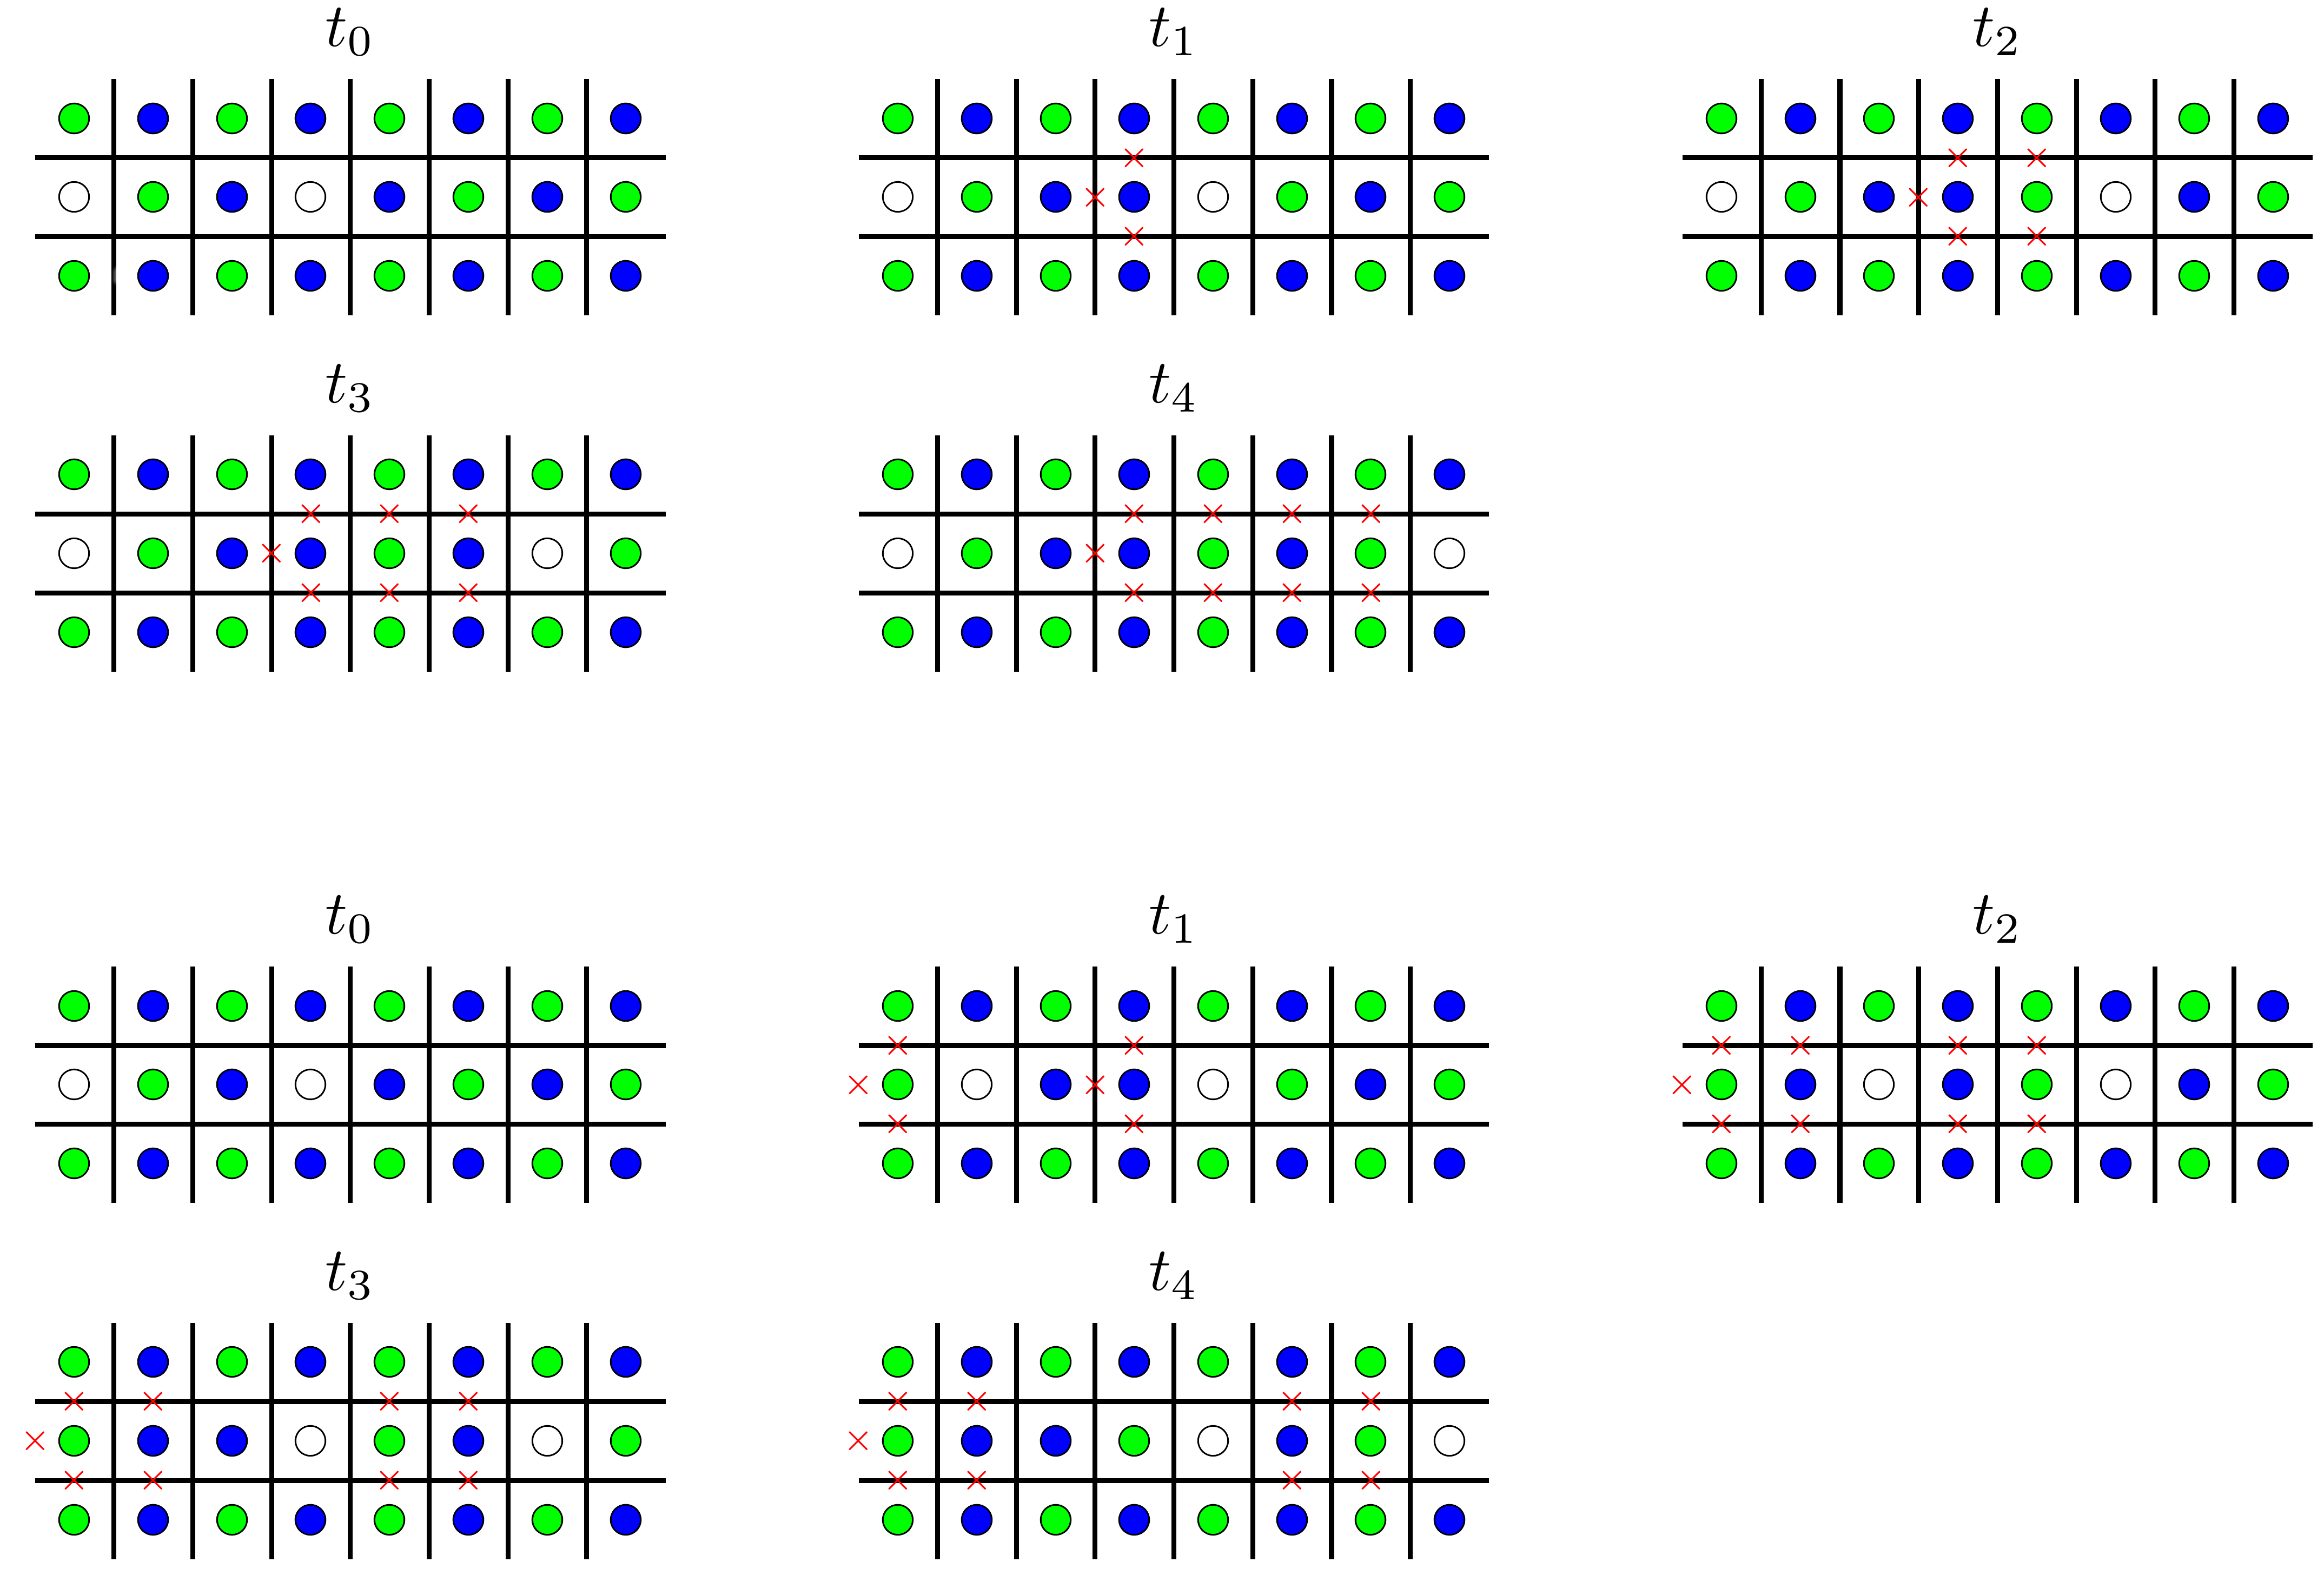
\includegraphics[width=\textwidth]{../illustrations/hole-pairing/pair_hopping.png}
\caption[Holes hopping in antiferromagnetic background.]{\small Energy
consideration for a pair of holes hopping in an antiferromagnetic background.
Spins up and down are represented as green and blue circles, holes are
represented as empty circles, and broken antiferromagnetic (AF) bonds are shown
as red crosses.  In the top series, every time the hole tunnels to an adjacent
site it breaks more AF bonds, which cost an energy $\approx -4t^{2}/{U}$ per
bond.  As the hole continues to hop, the total energy cost will be proportional
to the number of sites it has traveled.  In the bottom series, hopping is
correlated for the two holes; they hop together in the same direction.  In this
case, the energy cost of hopping will be proportional to the separation between
holes,  and it will not continue to grow as the holes move along further.   One
can see that the number of broken bonds is the same in going from $t_{3}$ to
$t_{4}$.  In the hole-doped antiferromagnet, if the kinetic energy decrease
from hole delocalization (tunneling) exceeds the cost of the broken AF bonds,
an insulating state may be able to lower its energy via the formation of
hole-pairs, } 
\label{fig:holepairing} 
\end{figure}

The arguments shown so far, regarding the symmetry of the ground states in a
4-site plaquette, and the effective attraction (or correlation) between holes
in an antiferromagnetic background, signal the close relationship between
antiferromagnetism and superconductivity.   To balance out the perspective on
this highly debated issue, we point out that in the phase diagram of
high-$T_{c}$ cuprates the  phase transition does not occur directly from an AFM
phase to a superconducting phase (the system must go through the pseudo-gap
regime as hole-doping is increased).  So if there is an AFM background in high
temperature superconductors, it may be of a different nature than the Mott
insulator type of AFM state which arises naturally in the Hubbard model. 


We hope that the simplified treatments of the Hubbard model presented so far
illustrate the richness of behaviors that emerge from it.   We have seen the
appearance of the Mott-Hubbard gap both in a single site, a double well, and a
4-site plaquette.  In the plaquette scenario we motivated the role of the
Hubbard model as one of the strongest candidates to describe the physics of
$d$-wave superconductivity in the cuprates. 
 

\section{ High-temperature series expansion } 


After exploring a few of the properties of the Hubbard model with overly
simplified approaches, we now turn to a method that will prove very useful in
comparing with experimental measurements.   The high-temperature series
expansion (HTSE) deals with tunneling as a perturbation on the on-site
interactions, and is thus the natural next step beyond the single site
treatment.  

 The partition function for the system is expanded as a series in the small
parameter $t/T$.   Clearly, this approach will work down to temperatures that
approach the tunneling rate, $T \gtrsim t$. We will see that this limits its
applicability to the calculation of thermodynamic quantities that involve the
charge degree of freedom, i.e. the density, double-occupancy, and their
derivatives.   The spin degree of freedom becomes relevant only at temperatures
below the antiferromagnetic exchange energy, which is much lower than $t$. 

We start by writing down the Hubbard Hamiltonian as  
\begin{equation}
\begin{split}
  H = &  
         \left( U\sum_{i} n_{i\spup} n_{i\spdn}  
         - \mu\sum_{i}( n_{i\spup} + n_{i\spdn} ) \right)
-t \sum_{ \langle ij \rangle, \sigma   } 
          a_{i\sigma}^{\dagger}a_{j\sigma} \\
   = &  H_{0} + H_{1} 
\end{split}
\end{equation}
We have already seen (in our treatment of the single-site model) that the
partition function for the unperturbed part, $Z_{0} = \text{Tr} e^{-\beta
H_{0}}$, factorizes as $Z_{0} = z_{0}^{k}$, for a system with $k$ sites.  The
single site partition function  is easy to calculate because the trace runs
over the only four possible states in a single site $\lbrace |0\rangle,
|\spup\rangle, |\spdn\rangle, |\dbl\rangle\rbrace$.
\begin{equation}
 z_{0} = 1 + 2 e^{\beta\mu} + e^{\beta (2\mu-U)} = 1 + 2z + z^{2}u 
\end{equation}
where we have defined $z=e^{\beta\mu}$ and $u=e^{-\beta U }$ 



For the full Hamiltonian, the grand canonical partition function $Z$ can be
expanded in a perturbation series~\cite{mahan2000many,Henderson1992} 
\begin{equation}
\begin{split}
  Z = & \text{Tr} e^{-\beta H}  \\
    = & Z_{0} \left[ 1 + 
        \sum_{n=1}^{\infty} (-1)^{n} 
        \int_{0}^{\beta} d\tau_{1} \int_{0}^{\tau_{1}} d\tau_{2} 
        \dotsm \int_{0}^{\tau_{n-1}} d\tau_{n} 
        \langle
              \tilde{H}_{1}(\tau_{1}) 
              \tilde{H}_{1}(\tau_{2})  \dotsm
              \tilde{H}_{1}(\tau_{n})  \rangle 
              \right] 
\end{split}
\end{equation} 
where the thermal expectation value inside the integrals is taken with the
unperturbed part of the Hamiltonian
\begin{equation}
\langle A \rangle = \text{Tr} ( e^{\beta H_{0} } A ) / Z_{0} , 
\end{equation}
and the tilde means that the operator is evaluated in the interaction picture
for the imaginary time in parenthesis: 
\begin{equation}
 \tilde{H}_{1}(\tau) = e^{\tau H_{0}} H_{1} e^{-\tau H_{0}} 
\end{equation}
Given the series expansion for $Z$, the grand potential is 
\begin{equation}
 -\beta \Omega = Z_{0} + 
        \sum_{n=1}^{\infty} (-1)^{n} 
        \int_{0}^{\beta} d\tau_{1} \int_{0}^{\tau_{1}} d\tau_{2} 
        \dotsm \int_{0}^{\tau_{n-1}} d\tau_{n} 
        \langle
              \tilde{H}_{1}(\tau_{1}) 
              \tilde{H}_{1}(\tau_{2})  \dotsm
              \tilde{H}_{1}(\tau_{n})  \rangle 
\end{equation}

One can see that the $n^{th}$ term in the expansion has $n$ copies of the
tunneling part of the Hamiltonian.  In the thermal average, each  application
of $H_{1}$ results in a particle tunneling to a neighboring site. We see that
there will be a contribution to the expansion only if after $n$ tunneling
events all the particles come back to their original sites.  A direct
consequence of this is that the first order term in the expansion vanishes (you
cannot recover the same lattice configuration after a single tunneling event).
The second order in the expansion corresponds to particles tunneling one site
over and then coming back.  Higher order terms can be represented by diagrams,
to make them easier to keep track off.  The contribution from orders up to
$n=9$ is shown in~\cite{Henderson1992}.  Here we will use up to the second
order term to illustrate the phases that appear in the system.  

The grand potential to second order is~\cite{Henderson1992,Jordens2010} 
\begin{equation}
-\beta \Omega_{2} = k \ln z_{0} + k \left( \frac{\beta t }{z_{0}} \right)^{2} m 
        \left( z + z^{3} u + 2z^{2} \frac{1-u}{\beta U} \right) 
\end{equation} 
where $m$ is the number of nearest neighbors for each lattice site, which in
the simple cubic case is $m=6$.  We see that the grand potential is
proportional to the number of lattice sites, so we will obtain all the
thermodynamic quantities per lattice site. 

\begin{figure}
\centering
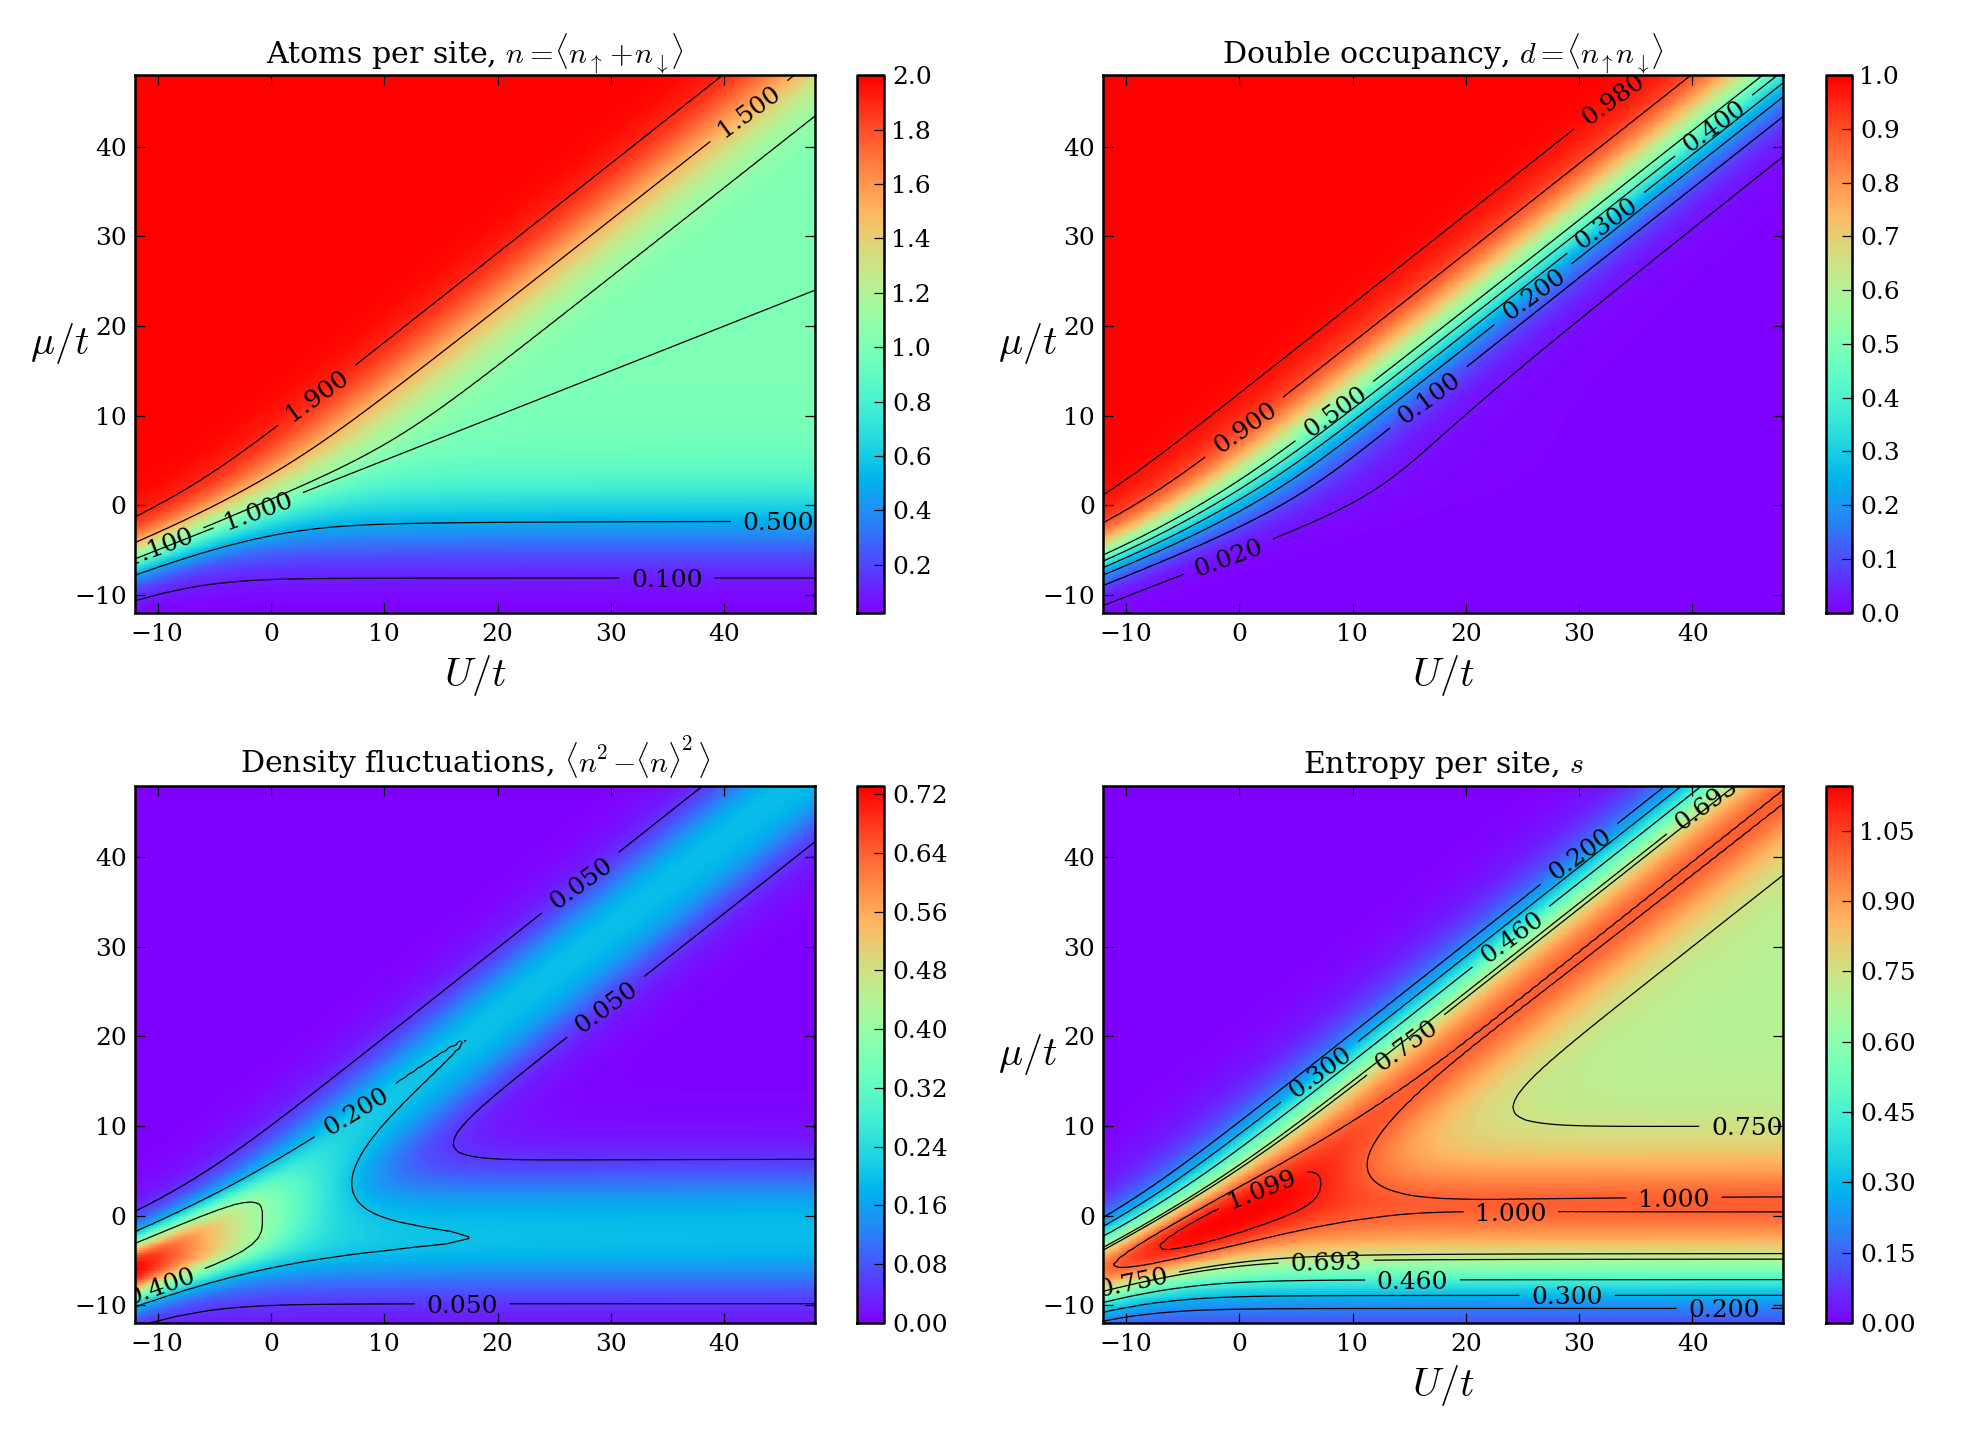
\includegraphics[width=\textwidth]{../figures/HubbardPhaseDiagram_figures/HTSE_phasesT025.png}
\caption[HTSE state diagram of the Fermi-Hubbard model]{\small HTSE state
diagram of the Fermi-Hubbard model calculated up to second order in the
perturbation series.  } \label{fig:highTphases}
\end{figure}
From the grand potential to second order we can calculate a state diagram for
the Hubbard model.  In Fig.~\ref{fig:highTphases}, the results are shown at a
temperature $T=2.5t$. Constant $T/t$ cuts are shown for different temperatures
in Fig.~\ref{fig:HTSEhomogeneous}.  

From the figures, we see that the HTSE up to second order exhibit the main
features of the Mott insulating regime: 
\begin{itemize}
\item The density as function of chemical potential has a
plateau at $n=1$ centered around $\mu=U/2$, Fig.\ref{fig:HTSEhomogeneousA}.
\item At $n=1$ the double occupancy
is suppressed for lower temperatures, Fig.~\ref{fig:HTSEhomogeneousB}.
\item
At $n=1$ the density fluctuations are suppressed, Fig.~\ref{fig:HTSEhomogeneousC}.
\item At $n=1$ the entropy per site is lowered,
Fig.~\ref{fig:HTSEhomogeneousD}.
\end{itemize}
For very large values of $U/t$, where at $T=2.5t$ we have $T \ll U$, the system
is deep in the Mott insulator regime.  The system has exactly one atom per
site, and the only remaining entropy is the spin entropy.  With two spin states
available per lattice site, the entropy per lattice site is $s = \ln 2 \approx
0.7 $, as can be seen in the third panel of Fig.~\ref{fig:HTSEhomogeneousD}.  

\begin{figure}
        \centering
        \begin{subfigure}[b]{0.48\textwidth}
                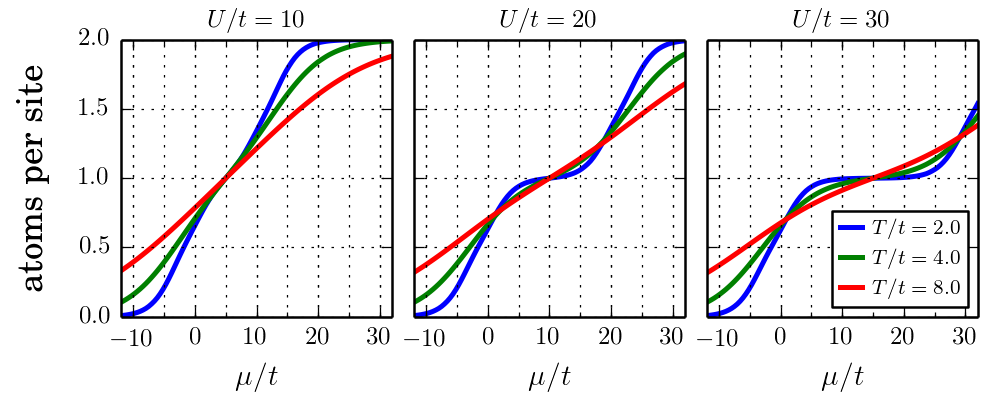
\includegraphics[width=\textwidth]{../figures/lda_evap/HTSE_density_U.png}
                \caption{Density}
\label{fig:HTSEhomogeneousA}
        \end{subfigure}%
          %add desired spacing between images, e. g. ~, \quad, \qquad etc.
          %(or a blank line to force the subfigure onto a new line)
        ~
        \begin{subfigure}[b]{0.48\textwidth}
                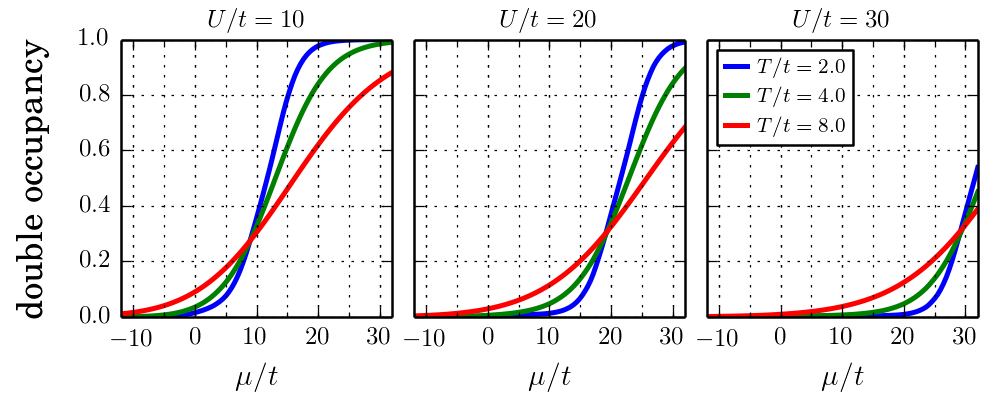
\includegraphics[width=\textwidth]{../figures/lda_evap/HTSE_doublons_U.png}
                \caption{Double occupancy}
\label{fig:HTSEhomogeneousB}
        \end{subfigure}

        \begin{subfigure}[b]{0.48\textwidth}
                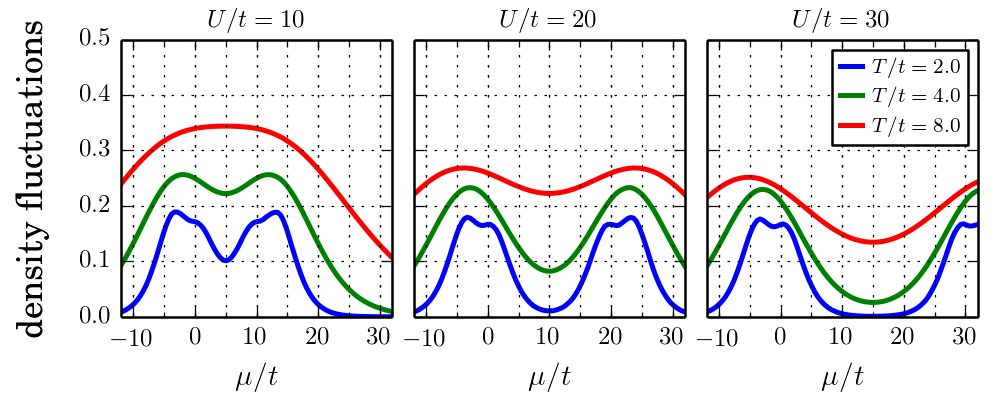
\includegraphics[width=\textwidth]{../figures/lda_evap/HTSE_densfluc_U.png}
                \caption{Density fluctuations}
\label{fig:HTSEhomogeneousC}
        \end{subfigure}
        ~
        \begin{subfigure}[b]{0.48\textwidth}
                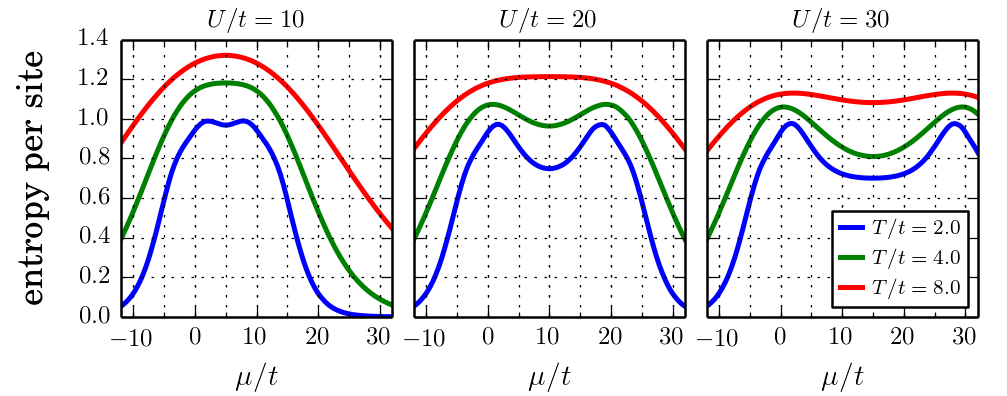
\includegraphics[width=\textwidth]{../figures/lda_evap/HTSE_entropy_U.png}
                \caption{Entropy per lattice site}
\label{fig:HTSEhomogeneousD}
        \end{subfigure}
        \caption{\small Thermodynamic quantities as a function of chemical potential calculated using the HTSE.}
\label{fig:HTSEhomogeneous}
\end{figure}


We can also plot the HTSE result for the entropy as a function of density, as
shown in Fig.~\ref{fig:HTSE_spersite}.  Dividing the entropy per lattice site
by the density, we obtain the entropy per particle, shown in
Fig.~\ref{fig:HTSE_sperparticle}.  The entropy per particle rises significantly
at lower densities, which indicates the large entropy capacity of the metallic
phase. 

\begin{figure}
        \centering
        \begin{subfigure}[b]{0.65\textwidth}
    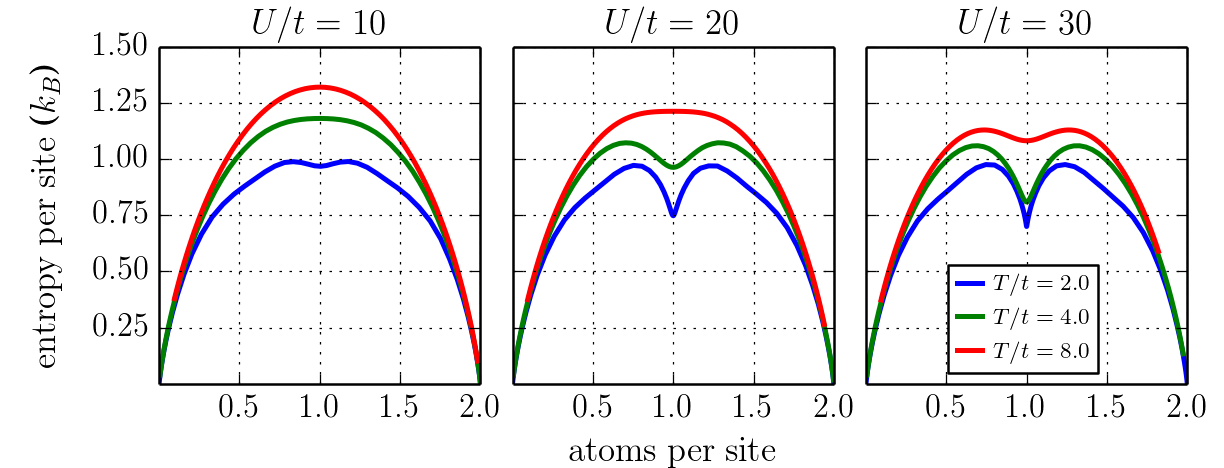
\includegraphics[width=\textwidth]{../figures/lda_evap/HTSE_EntropyPerSite_U.png}
    \caption{Entropy per lattice site versus density.}\label{fig:HTSE_spersite}
     \end{subfigure}

\begin{subfigure}[b]{0.65\textwidth}
    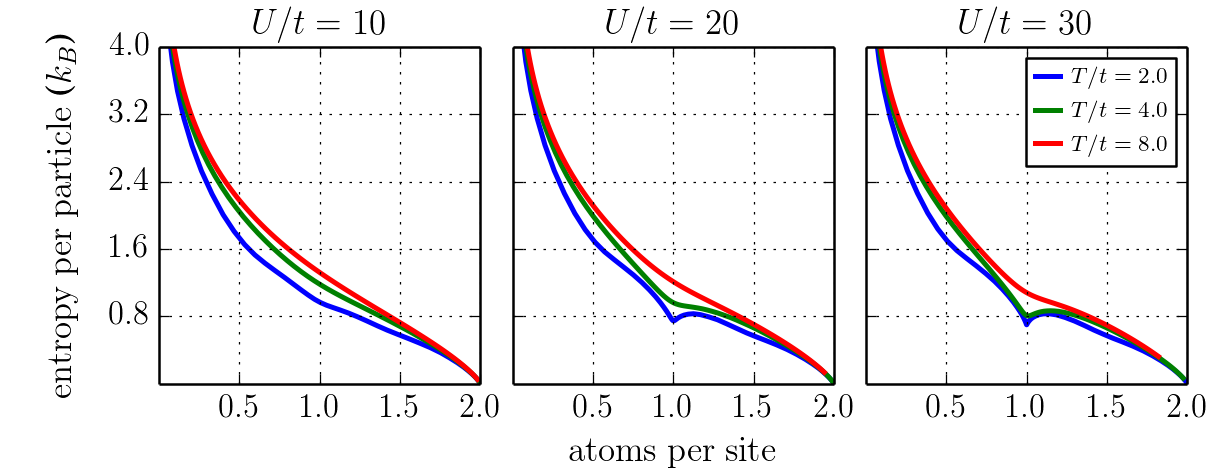
\includegraphics[width=\textwidth]{../figures/lda_evap/HTSE_EntropyPerParticle_U.png}
    \caption{Entropy per particle versus density.}\label{fig:HTSE_sperparticle}
   \end{subfigure}
\end{figure}

In a finite trapped system which inevitably has a shell with density $n<1$ , a
large part of the total entropy of the system is carried by particles in the
low density shell.  This \textbf{entropy redistribution} allows the core to be
at an effectively lower entropy per particle.  The core can then locally access
lower entropy phases, such as the AFM state,  even if the overall value of the
entropy per particle is larger than the N\'{e}el entropy for a homogeneous
system\footnote{ For the homogeneous system the N\'{e}el entropy per particle
(at which the Mott insulator becomes AFM ordered) is $s_{\text{N\'{e}el}} = 0.4
k_{\text{B}}$}.  We will elaborate more on this later on when we describe our
trapping potential. 


\section{ Local density approximation }

The results presented above consider a homogeneous lattice potential.  In
experiments with ultracold atoms,  a confining potential is a necessity since
the samples created have a finite number of atoms.  The presence of an
inhomogeneous overall trapping potential presents a major challenge when
comparing the results of experiment to theory.  A useful technique, which works
for systems without long range correlations, is the local density approximation
(LDA) .  In the LDA, we consider each point in the potential as an homogeneous
system and we set the condition that all of these local homogeneous systems are
in thermal equilibrium with each other  at some temperature $T$.  If the
trapping potential is properly characterized,  at each point we can obtain a
local value of the lattice depth, which along with the scattering length (set
for the whole system via a Feshbach resonance), determines the local values of
the Hubbard parameters $t$ and $U$.  With the Hubbard parameters in hand, we
can use a known solution to the homogeneous Hubbard model and obtain local
values for the thermodynamic quantities, such as density, double occupancy,
entropy, etc.   We can then plot the local thermodynamic quantities as a
function of trap position to obtain trap profiles.  Alternatively, one can also
integrate the results of the LDA over the trap and compare them to bulk
measurements. 


The validity of the LDA in lattice systems has been addressed
before~\cite{Rigol2003,Helmes2008,Chiesa2011},  proving that it yields very
good agreement with exact calculations of the trap for quantities such as
density profiles and momentum distributions and only slight discrepancies with
quantities like the spectral function of the many-body excitations.  In the
work carried out for this thesis, all the comparisons with theory were done
within the framework of the LDA. 


\section{Latest developments in numerical techniques}

When performing the LDA one needs to have available a set of results for a
homogeneous model with data available at low enough temperatures to match those
of the experiment.   In our experiment the temperature can be as low as
$T/t\approx0.4$ locally, just above $T_{N}$ and so we need to make use of the
latest developments in numerical techniques to access this regime.   The hope
is that one day ultracold atoms will greatly exceed the capabilities of
numerical calculations, such that open questions like that of $d$-wave
superconductivity in the Hubbard model can be put to rest. 

Going down to temperatures comparable to the tunneling rate ($T<t$), analytical
methods such as the HTSE up to second order fall short in their ability to
describe the thermodynamics of the Hubbard model.  Below these temperatures a
variety of more sophisticated approaches has been used in the literature.
Below we provide a non-exhaustive list of the main methods that have been
applied to ultracold atoms in optical lattices:  

\begin{itemize} 

\item \textbf{DMFT}.  Dynamical mean field theory. It considers a single site
of the lattice, $H_{1}= Un_{\spup}n_{\spdn} - \mu (n_{\spup} + n_{\spdn})$,
immersed in a bath of non-interacting electrons which represents the rest of
the system.   The interaction between the bath and the impurity is mapped onto
what is referred to as a single-impurity Anderson model.    The resulting
impurity model is solved with a self-consistency condition, i.e.  the resulting
dynamics of the bath must be consistent with the dynamics of the impurity
since, after all, the bath is made of a bunch of other sites, just like the one
under consideration.  Of course, this is easier said than done; nevertheless,
the problem reduces to solving the problem for a single-impurity.  There are
several techniques available for that task.  Ref.~\cite{Helmes2008} uses the
numerical renormalization group (NRG), for example. 


\item \textbf{DCA}.  Dynamical cluster approximation.  This is an extension of
DMFT, where the impurity is not a single site but a cluster of sites.  As the
number of sites in the cluster, $N_{c}$ goes to infinity one should recover the
exact solution, and for $N_{c}=1$ the method reduces to DMFT.   The DCA was used
to calculate the thermodynamics of the Fermi-Hubbard in a 3D lattice in
Ref.~\cite{Fuchs2011}.

\item \textbf{DQMC}.  Determinantal quantum Monte Carlo.  In general, the Monte
Carlo  method reduces the calculation of the full quantum partition function as
a sum over all possible configurations in some product space basis set (where
the basis states are products of single particle states).  In
DQMC~\cite{Scalettar:hubbardIII,PhysRevD.24.2278}, an exact simplification is
used where the partition function is reduced to a sum over the determinant of
the Hamiltonian matrix (in the chosen basis).  So the name ``determinantal''
QMC.  This simplification holds if the Hamiltonian is quadratic.  The on-site
interaction term in the Hubbard model is quartic instead of quadratic, but
there is a way to handle this using what is called a Hubbard-Stratonovich
transformation.  A problem with applying this method to fermions is that the
determinant of the resulting matrices can be negative sometimes, which affects
the convergence of the Monte Carlo evaluation of the sum.   This is known as
the sign problem,  it can be avoided completely for calculations at
half-filling ($\mu=U/2$) and it is not so significant for small values of $U$ at
arbitrary filling.  However, for large values of $U \gtrsim 12$ it prevents
calculations for values of $T/t \lesssim 1$. 

\item \textbf{NLCE}. Numerical linked-cluster expansion.   The NLCE is a series
expansion in powers of $t/T$, which reminds one of the HTSE.  In the HTSE,
different contributions are grouped solely by the power of $t/T$, whereas in
the NLCE clusters of sites are exactly diagonalized (numerically) and added to
the series according to a weight that can be obtained by a considering all
possible subclusters in the cluster~\cite{PhysRevLett.97.187202}.   The region
of convergence of the NLCE can be extended for  $T/t<1$ via numerical
resummations~\cite{Tang2013}, although results for $T/t<0.8$ in a 3D lattice
can get rather noisy, as we will see. 

\end{itemize}

As part of this thesis we have closely collaborated with the following condensed matter theorists:
\begin{itemize}
\item Thereza Paiva at Universidade Federale de Rio de Janeiro  
\item Ehsan Khatami at San Jose State University
\item Richard Scalettar at UC Davis
\item David Huse at Princeton University
\item Nandini Trivedi at Ohio State University
\end{itemize}  

Our collaborators are experts in the use of DQMC and NLCE and so all of the
modeling of our experimental results is restricted to these two techniques.

%%%%%%%%%%%%%%%%%%%%%%%%%%%%%%%%%%%%%%%%%%%%%%%%%%%%%%%%%%%%%%%%%%%%%%%%%%%%%%%
%%%%%%%%%%%%%%%%%%%%%%%%%%%%%%%%%%%%%%%%%%%%%%%%%%%%%%%%%%%%%%%%%%%%%%%%%%%%%%%
%%%%  CHAPTER 4   
%%%%%%%%%%%%%%%%%%%%%%%%%%%%%%%%%%%%%%%%%%%%%%%%%%%%%%%%%%%%%%%%%%%%%%%%%%%%%%%
%%%%%%%%%%%%%%%%%%%%%%%%%%%%%%%%%%%%%%%%%%%%%%%%%%%%%%%%%%%%%%%%%%%%%%%%%%%%%%%
\chapter{Overview of the experimental setup}
\label{chap:setup-overview}

In this chapter we will give a brief description of the experimental setup used
for this thesis.  The idea is to make the reader familiar with the experimental
steps required to produce an ultracold Fermi gas and the different systems
associated with each step,  before explaining concepts in more detail in later
chapters.  We will assume familiarity with the use of light to cool and trap
atoms~\cite{RevModPhys.70.685,RevModPhys.70.707,RevModPhys.70.721},  and with
the use of magnetic fields to control the strength of the interactions between
atoms~\cite{RevModPhys.82.1225}. 

For the non-expert, it will suffice to know that light that is near resonant to
an atomic transition can result in dissipative forces, which can be used to
reduce the velocity of atoms (cooling).  Light detuned far from an atomic
transition produces a conservative force,  which changes the potential energy
of an atom.  If the far detuned light is detuned to the red of the atomic
transition, atoms will be attracted to intensity maxima of the light field
(trapping), whereas if the light is red detuned they will be repelled from the
intensity maxima. 


It takes about 15 seconds to produce a degenerate cloud of \li\ atoms.  It then
takes only a few tens of milliseconds to load this cold sample into an optical
lattice and perform a measurement on it.  Measurements are destructive, so we
must repeat the process over and over again.   Most of the time in the lab is
spent optimizing the setup and finding out the right way to carry out the
experiments.   Final data can then consist of only a few tens to a few hundred
shots, depending on the statistics needed for the particular experiment. 

In Fig.~\ref{fig:vacuum} we show a schematic of the vacuum system where the
experiments are carried out.  This will give the reader a spatial setting in
which to visualize the descriptions given below.  The experimental cycle
proceeds in the following way:  
\begin{enumerate} 
\item A thermal beam of \li\ atoms, which originates at the oven, is
decelerated by near-resonant counter-propagating light.  A tapered solenoid is
used to produce a spatially varying magnetic field used to compensate the
changing Doppler shift as the atoms decelerate.   This scheme is referred to as
Zeeman slowing.  After the Zeeman slower, the atoms are  cooled transversally
by the two-dimensional magneto-optical trap (2DMOT). 

\item  The magneto-optical trap (MOT) captures the slowed atoms at the center
of the chamber, where they reach a temperature as low as $\sim300~\mu$K.  

\item  We transfer the atoms from the MOT to a narrow linewidth magneto-optical
trap, which operates on the ultraviolet \uv\ transition (UVMOT).  In the UVMOT
the atoms are cooled down to $\sim60~\mu$K.  

\item  We load a balanced mixture of atoms in the two lowest energy hyperfine
states into a crossed-beam optical dipole trap (ODT)

\item  Once in the ODT, a magnetic field is used to control the scattering
cross section between atoms in the two different hyperfine states, via a
magnetic Feshbach resonance~\cite{Houbiers1998}.   Setting a large scattering
cross section allows efficient evaporative cooling to quantum degeneracy.
Cooling is forced by reducing the depth of the optical potential. 

\item As the power in the ODT is reduced for evaporation, the atoms are left in
a dimple trap,  which was ramped up prior to the start of evaporation.   The
dimple trap is the starting point in all of our experiments.   

\item At this point, the trapping potential is slowly transformed into an
optical lattice potential, where the Hubbard model is realized. We then proceed
to measure the properties of the system.  
\end{enumerate}

In the following sections we briefly describe the different systems involved in
the realization of the experimental cycle. 


%########################################
\section{Vacuum system}
%########################################

\begin{figure}
\centering 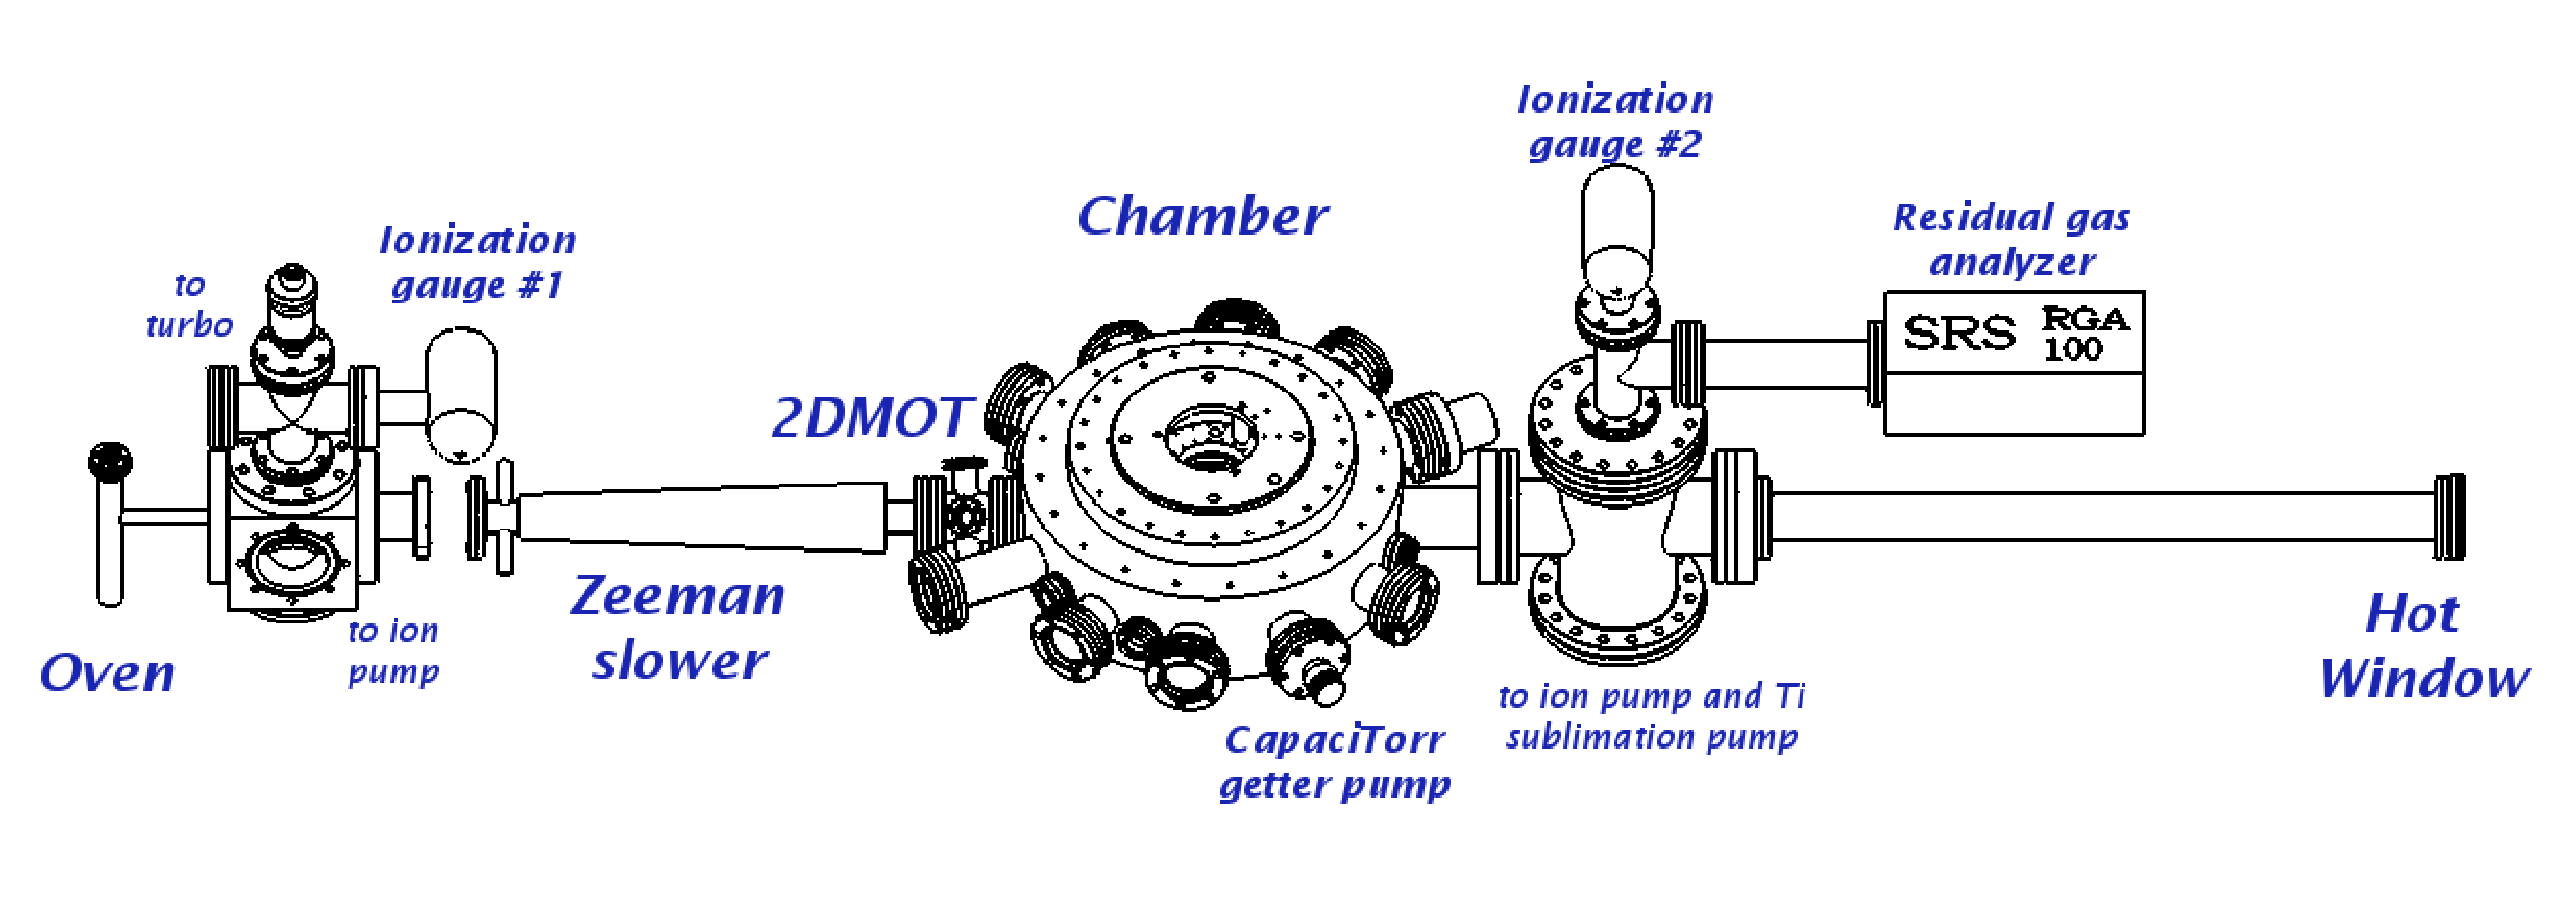
\includegraphics[width=\textwidth]{../masters-figures/vacuum/vacuum02.pdf}
\caption[Apparatus3 vacuum system]{\small Main components of the
vacuum system. } \label{fig:vacuum}
\end{figure}
During operation, the oven section of the vacuum system (see
Fig.~\ref{fig:vacuum}) is heated to 450$^{\circ}$C to produce a collimated beam
of lithium atoms.  The Zeeman slower (described later in
Sec.~\ref{subsec:zeemanslower}) is constructed with a narrow tube and provides
a low conductance (0.5~L/s) that can help maintain 
%up to a factor of 10
a pressure differential between the oven and the main chamber sections.  The
pressure\footnote{Measured with Bayard-Alpert type ionization gauge (Varian
Type 571) labeled \#1 in Fig.~\ref{fig:vacuum}} in the oven section is $4\times
10^{-9}$~Torr, and in the chamber section\footnote{Measured with ion gauge \#2}
is $<5\times10^{-10}$~Torr.   

Lithium atoms that are not captured by the MOT eventually hit a sapphire window
at the far end of the setup, which we refer to as the `hot window' because it
is heated up to around 290$^{\circ}$C to avoid coating it with the lithium
metal.  The long tube between the chamber and the hot window serves a
differential pumping purpose; the tube inside is lined with a helical strip of
non-evaporable getter material\footnote{SAES St 707/CTAM/30D, 30~mm wide
strip.}.

The vacuum is maintained by two ion pumps and a non-evaporable getter pump.  A
VacIon Plus Starcell (150~L/s) from Varian vacuum technologies is connected to
the cross between the chamber and the hot window sections.   A titanium
sublimation cartridge is attached to this pump.  A
smaller Vacion Plus Starcell (55~L/s) is connected to the cube on the oven
section.  A CapaciTorr B200 getter pump (90~L/s for H$_{2}$) is attached
directly to one of the chamber viewports.   Due to the close proximity of this
getter pump to the atoms (8~cm) we expect the background pressure to be lower
in the center of the chamber than the $5\times10^{-10}$~Torr measured with ion
gauge \#2.



%########################################
\section{671 nm laser cooling system}
%########################################


For the Zeeman slower, 2DMOT and MOT we perform laser cooling using the \red\
transition in \li\ (see level diagram in Fig.~\ref{fig:671levels}) which has a
wavelength of 671~nm.    The light is produced in a separate optical table and
transferred to the apparatus table via optical fibers.  In this section we give
a description of the different parts of the 671~nm laser cooling system.  

%On the apparatus table, the MOT light is split into
%six beams and the correct circular polarizations are set.  In this section I
%describe the laser system used to produce the light for the MOT and the Zeeman
%slower, and also give technical information about our Zeeman slower.  Details
%about the operation parameters and characteristics of the MOT are deferred to
%Chapter~\ref{ch:uvmot}.


%----------------------------------------
\subsection{Laser system}
%----------------------------------------

\begin{figure} \centering
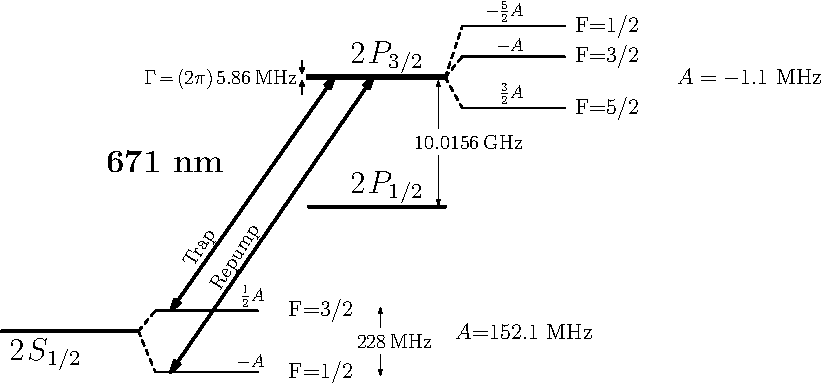
\includegraphics[width=0.85\textwidth]{../masters-figures/levels/671-levels/lithium.pdf}
\caption[Lithium-6 energy level diagram]{\small Energy level diagram showing
transitions relevant for laser cooling \li using the \red transition. }
\label{fig:671levels} \end{figure} 

Efficient laser cooling relies on continuous scattering of photons by the atom.
To avoid optical pumping to a dark hyperfine ground state we use two
frequencies of light, tuned to the $\twos{1/2}\cm\f{3/2}$ and
$\twos{1/2}\cm\f{1/2}$ states.  We refer to these as trap and repump,
respectively, as shown in Fig.~\ref{fig:671levels}. 

%  In a magneto-optical trap, a lithium atom,
%see Fig.~\ref{fig:671levels}, that absorbs a photon on the
%$\twos{1/2}\cm\f{3/2}\rightarrow\twop{3/2}$ transition, referred to as the
%trapping transition, can decay to the
%$\twos{1/2}\cm\f{1/2}$ state.  To maintain the continuous scattering of photons, a
%second frequency that is tuned to the
%$\twos{1/2}\cm\f{1/2}\rightarrow\twop{3/2}$ transition is required; we refer to
%this transition as the repumping transition.  The probability of going to a
%dark state is higher in lithium than in other alkalis such as rubidium, cesium,
%or sodium  because the hyperfine structure of the excited state is unresolved,
%$\Gamma\approx 5|A|$. 

%\begin{sidewaysfigure} \centering
%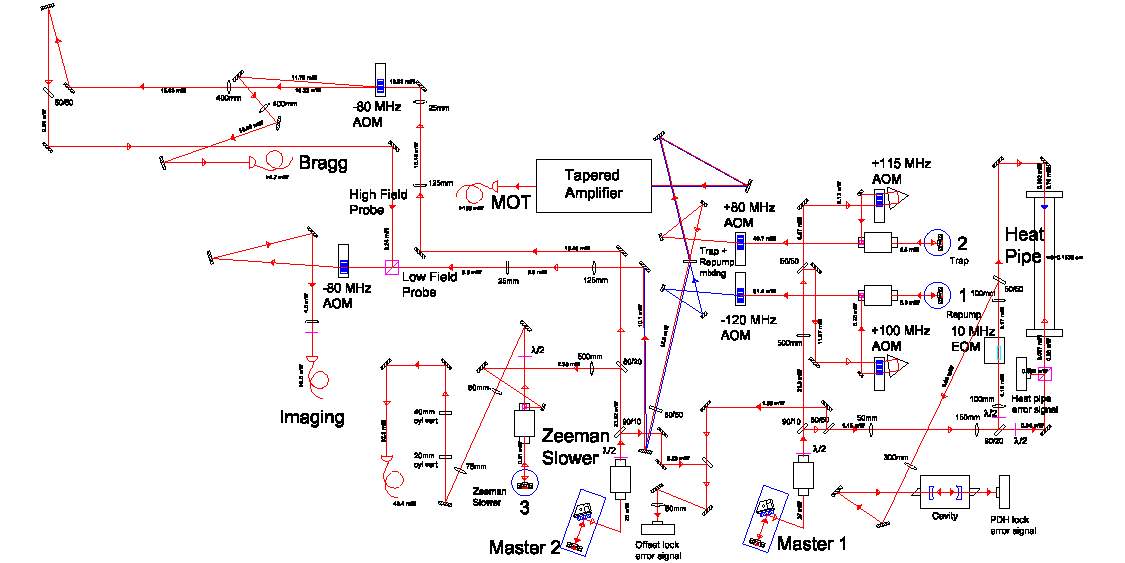
\includegraphics[width=1.\textwidth]{../masters-figures/671setup/671setup(v4).pdf}
%\vspace{1cm} \par \caption[671 nm laser system]{\small Intended for the in
%house reader, this figure shows the layout of the Apparatus3 671 nm laser
%system.  Benchmark powers are indicated on the figure.  } \label{fig:671system}
%\end{sidewaysfigure} 

The laser system that is used to produce the trapping and repumping MOT light,
as well as the Zeeman slower and imaging probe light, was described in detail
in my Master's thesis~\cite{DuarteMs}.    We have two home-built extended
cavity diode lasers, which we refer to as MOT~Master and ZS~Master. The
MOT~Master is stabilized to the $\twos{1/2}\cm\f{3/2}\rightarrow\twop{3/2}$
transition via saturated absorption spectroscopy and the ZS~Master is offset
locked (red detuned) to the MOT~Master using the side-of-filter
technique~\cite{SoftLock2004}.  

\subsubsection{MOT~Master} 

Light from the MOT~Master is split up for producing the trap and repump
frequencies; each path is passed through a double-pass acousto-optic modulator
(AOM) and injection-locks a slave laser diode for amplification.  The light
from the trap and repump slaves is overlapped on a beamsplitter before
injecting a tapered amplifier.  The output from the tapered amplifier is fiber
coupled to the apparatus table.  After passing through an AOM and splitting ten
percent of the light for the 2DMOT, we can get as much as 90 mW of power for
the MOT.   Due to the small splitting between trap and repump frequencies, 22
mW of light are produced by the tapered amplifier in unwanted sidebands at
\mbox{$f_{\mathrm{trap}}-228\,\mathrm{MHz}$} and
\mbox{$f_{\mathrm{repump}}+228\,\mathrm{MHz}$}~\cite{Ferrari1999}. This results
in a net 53~mW of trapping light and 16~mW of repumping light that are
dedicated to the MOT.  

\subsubsection{ZS~Master}
 
Light from the ZS~Master is split up into two paths.  The first path is used as
the probe light in Bragg scattering experiments. It is passed through AOMs for
power control and switching purposes and coupled into an optical fiber.
Approximately 5 mW are available for the experiment at the output end.  The
second path is used to inject a slave laser diode for amplification.  The
output of the slave passes through an AOM, which selects whether the light is
used for Zeeman slowing or imaging.  The zeroth order of the AOM is used for
Zeeman slowing and the 1st order is used as the imaging probe.   Approximately
30~mW (20~mW)  of light are available for Zeeman slowing (imaging) after the
light is coupled into an optical fiber.    

%Besides the loss of power we have not observed negative
%effects in the operation of the MOT from the presence of the sideband
%frequencies created by the tapered amplifier.
%
%The ZS~Master is used to produce the Zeeman slower light and the imaging probe.
%Light from the ECDL is  split into two paths:  the first path injects a slave to
%produce the Zeeman slower light, the second path is diverted to the imaging
%setup.   The light from the Zeeman slower slave is coupled to an optical fiber
%to be transferred to the apparatus table.   Light that goes to the imaging
%setup is passed through an AOM and coupled to a fiber to be used as the probe
%light for atoms at high magnetic field.   
%
%\begin{figure} \centering
%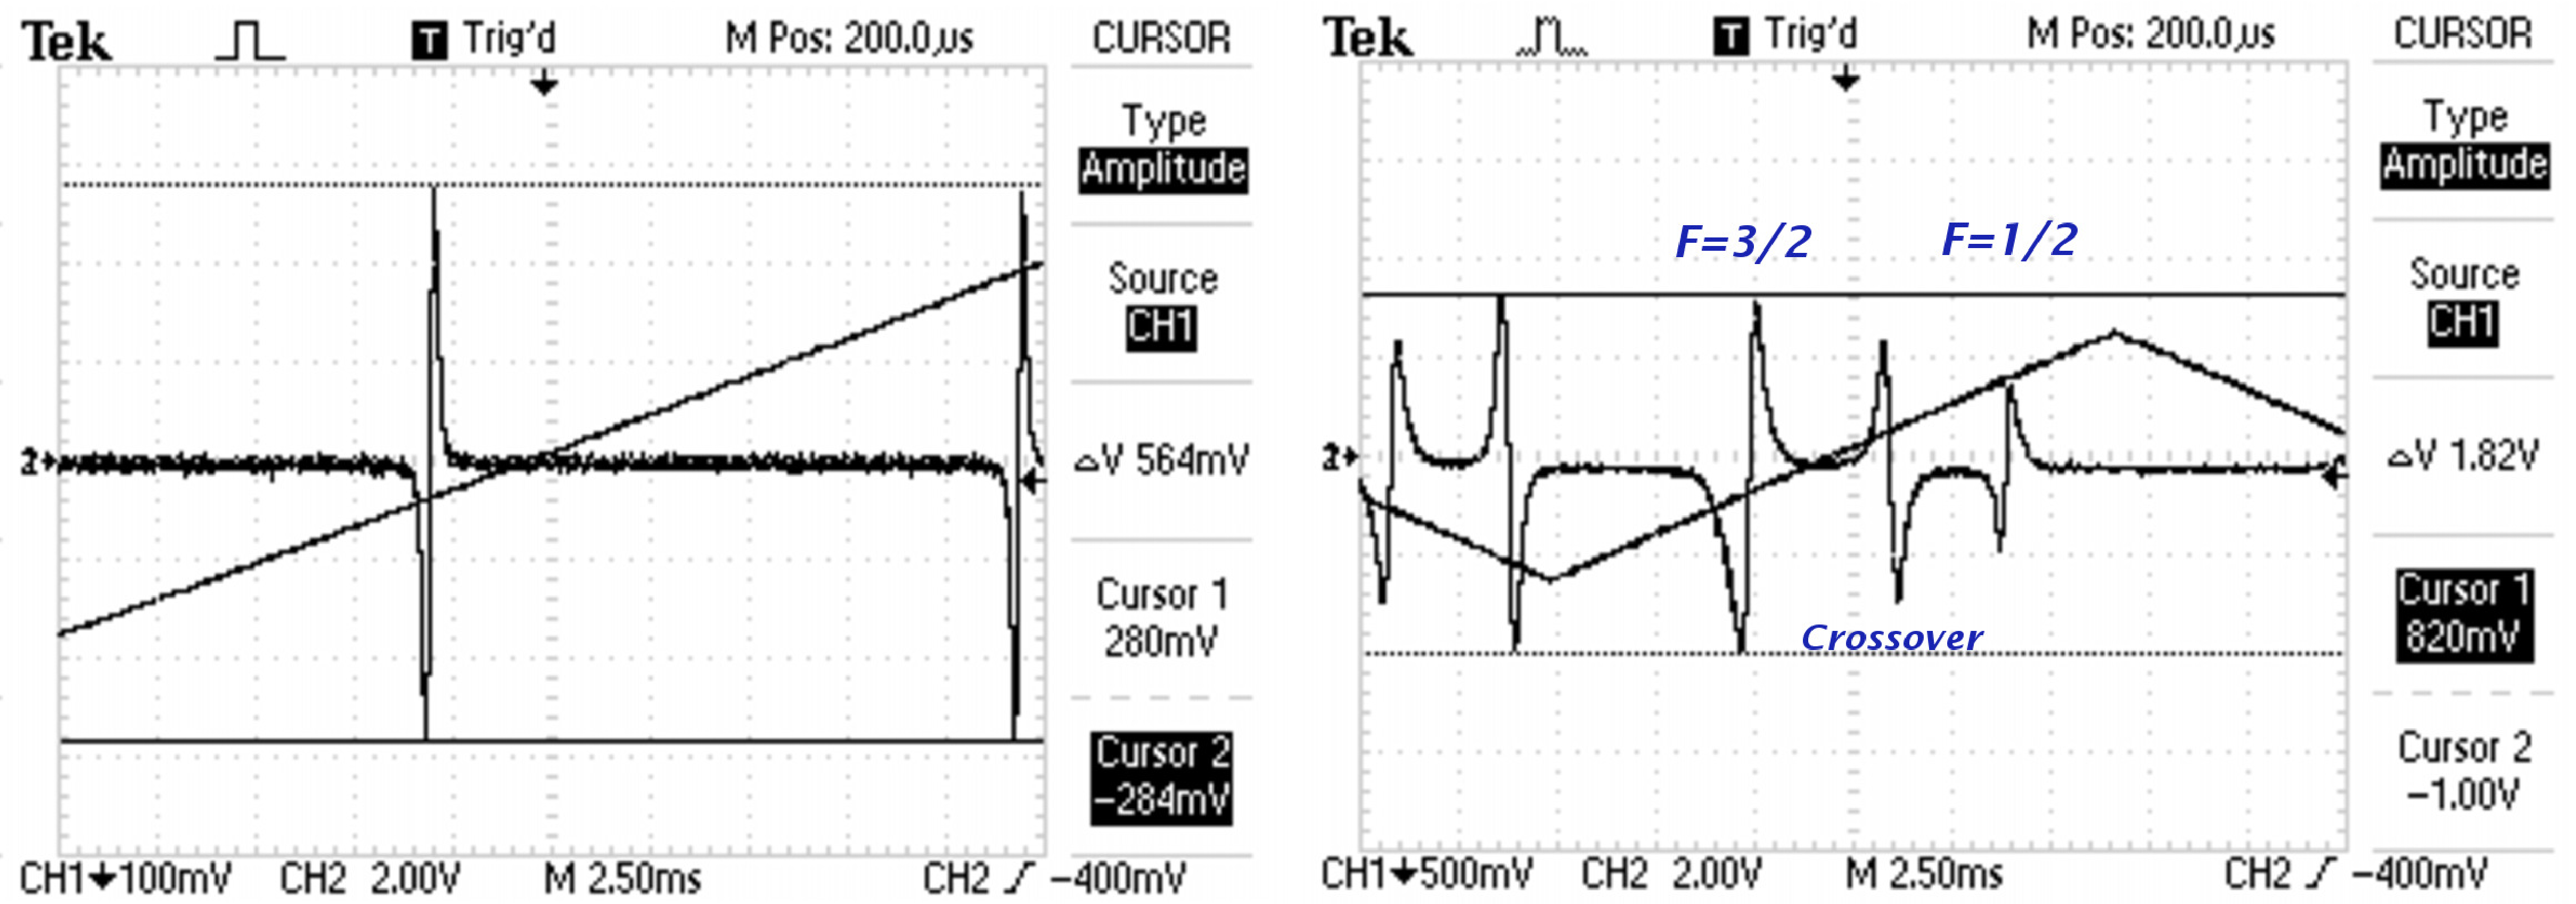
\includegraphics[width=0.95\textwidth]{../masters-figures/671setup/MotMaster.pdf}
%\caption[Lock error signals for  671 nm MOT~Master]{\small The MOT~Master is
%stabilized to the error signal from a Fabry-Perot cavity (left). The cavity is
%stabilized using a saturated absorption spectroscopy error signal obtained from
%a lithium heat pipe.  To obtain both of the error signals shown in this figure
%the Pound-Drever-Hall (PDH) technique is used, where the necessary sidebands
%are produced by phase modulation with an electro-optic modulator at 13 MHz. }
%\label{fig:motmaster} \end{figure}
%
%\begin{figure} \centering
%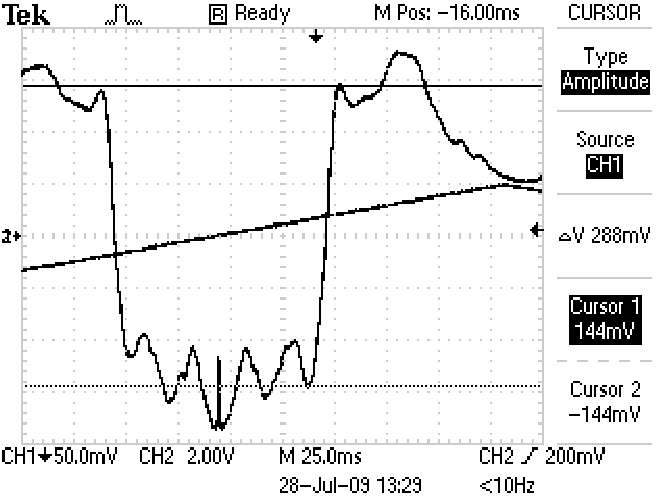
\includegraphics[width=0.475\textwidth]{../masters-figures/671setup/offsetlock.pdf}
%\caption[Side of filter lock error signal for 671 nm ZS~Master]{\small The
%ZS~Master is stabilized using an error signal obtained using the side-of-filter
%technique.   The zero crossing of the error signal is determined by the
%frequency of a local oscillator which can be tuned.  In our setup we can tune
%ZS~Master from -400 MHz to -1500 MHz with respect to  MOT~Master.  }
%\label{fig:zsmaster} \end{figure}

	
%----------------------------------------
\subsection{Zeeman slower}
\label{subsec:zeemanslower}
%----------------------------------------
The Zeeman slower reduces the speed of atoms coming out of the oven to less
than the capture velocity of our MOT, $v_{\mathrm{c}}\simeq 5\Gamma/k = 20$
m/s, where $5\Gamma$ is the red detuning from resonance at which we operate the
MOT during loading. The Zeeman slower works by using red detuned laser light
propagating opposite to the lithium atomic beam.  Due to the Doppler shift, the
laser light is resonant with atoms coming out of the oven, and via repeated
photon scattering can produce a maximum deceleration given by $a_{\mathrm{max}}
= \frac{h\Gamma}{2\lambda m}$.  As the atoms get slowed they shift out of
resonance, but the spatially dependent magnetic field of the Zeeman slower
shifts the transition to the red keeping the atoms resonant with the light as
they travel through the slower.

The Zeeman slower operates on the $\sigma^{-}$  transition between the
$\twos{1/2}\cm\f{3/2}\cm\mf{-3/2}$ and $\twop{3/2}\cm\f{5/2}\mf{-5/2}$ levels,
shown in red in Fig.~\ref{fig:zeemanlevels}. An advantage of choosing this
transition is that it is a cycling transition even at moderate magnetic fields.
This eliminates the need for using repumping light in the Zeeman slower.  
\begin{figure}
\centering
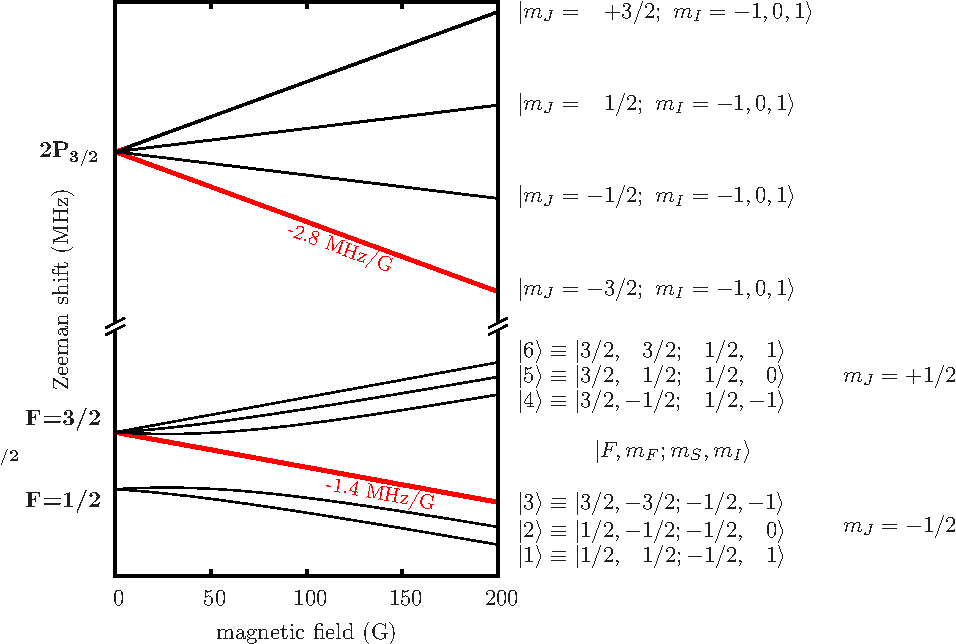
\includegraphics[width=1.0\textwidth]{../masters-figures/levels/zeeman_revised/01eps.pdf}
\caption[Levels of \li in a magnetic field. ]{\small Energy level diagram of
\li in a magnetic field.   The red lines show the levels used in the Zeeman
slower.  } \label{fig:zeemanlevels} 
\end{figure} 
We use a detuning of 1312~MHz, and a magnetic field profile given by \[ B_{z} =
B_{0}(1-\sqrt{1-z/L}) \] where $B_{0}\approx800$~G and $L=34.5$~cm.   



%----------------------------------------
\subsection{2DMOT and MOT}
%----------------------------------------
The 671 nm MOT is loaded from a Zeeman slower plus a 2DMOT. The 2DMOT is at the
output of the Zeeman slower and helps collimate the slow thermal beam of atoms
before it reaches the MOT.   The 2DMOT consists of a quadrupole field with two
pairs of counter-propagating beams which lie on a plane almost normal to the
direction of propagation of the atomic beam.   In our setup, the atomic beam is
offset from the center of the chamber by $\sim1\,$cm, and the angle of the
2DMOT is such that the slowed atoms from the Zeeman slower will be redirected
towards the MOT, located at the center of the chamber (see
Fig.~\ref{fig:apparatus-schem}). 
\begin{figure}
\centering
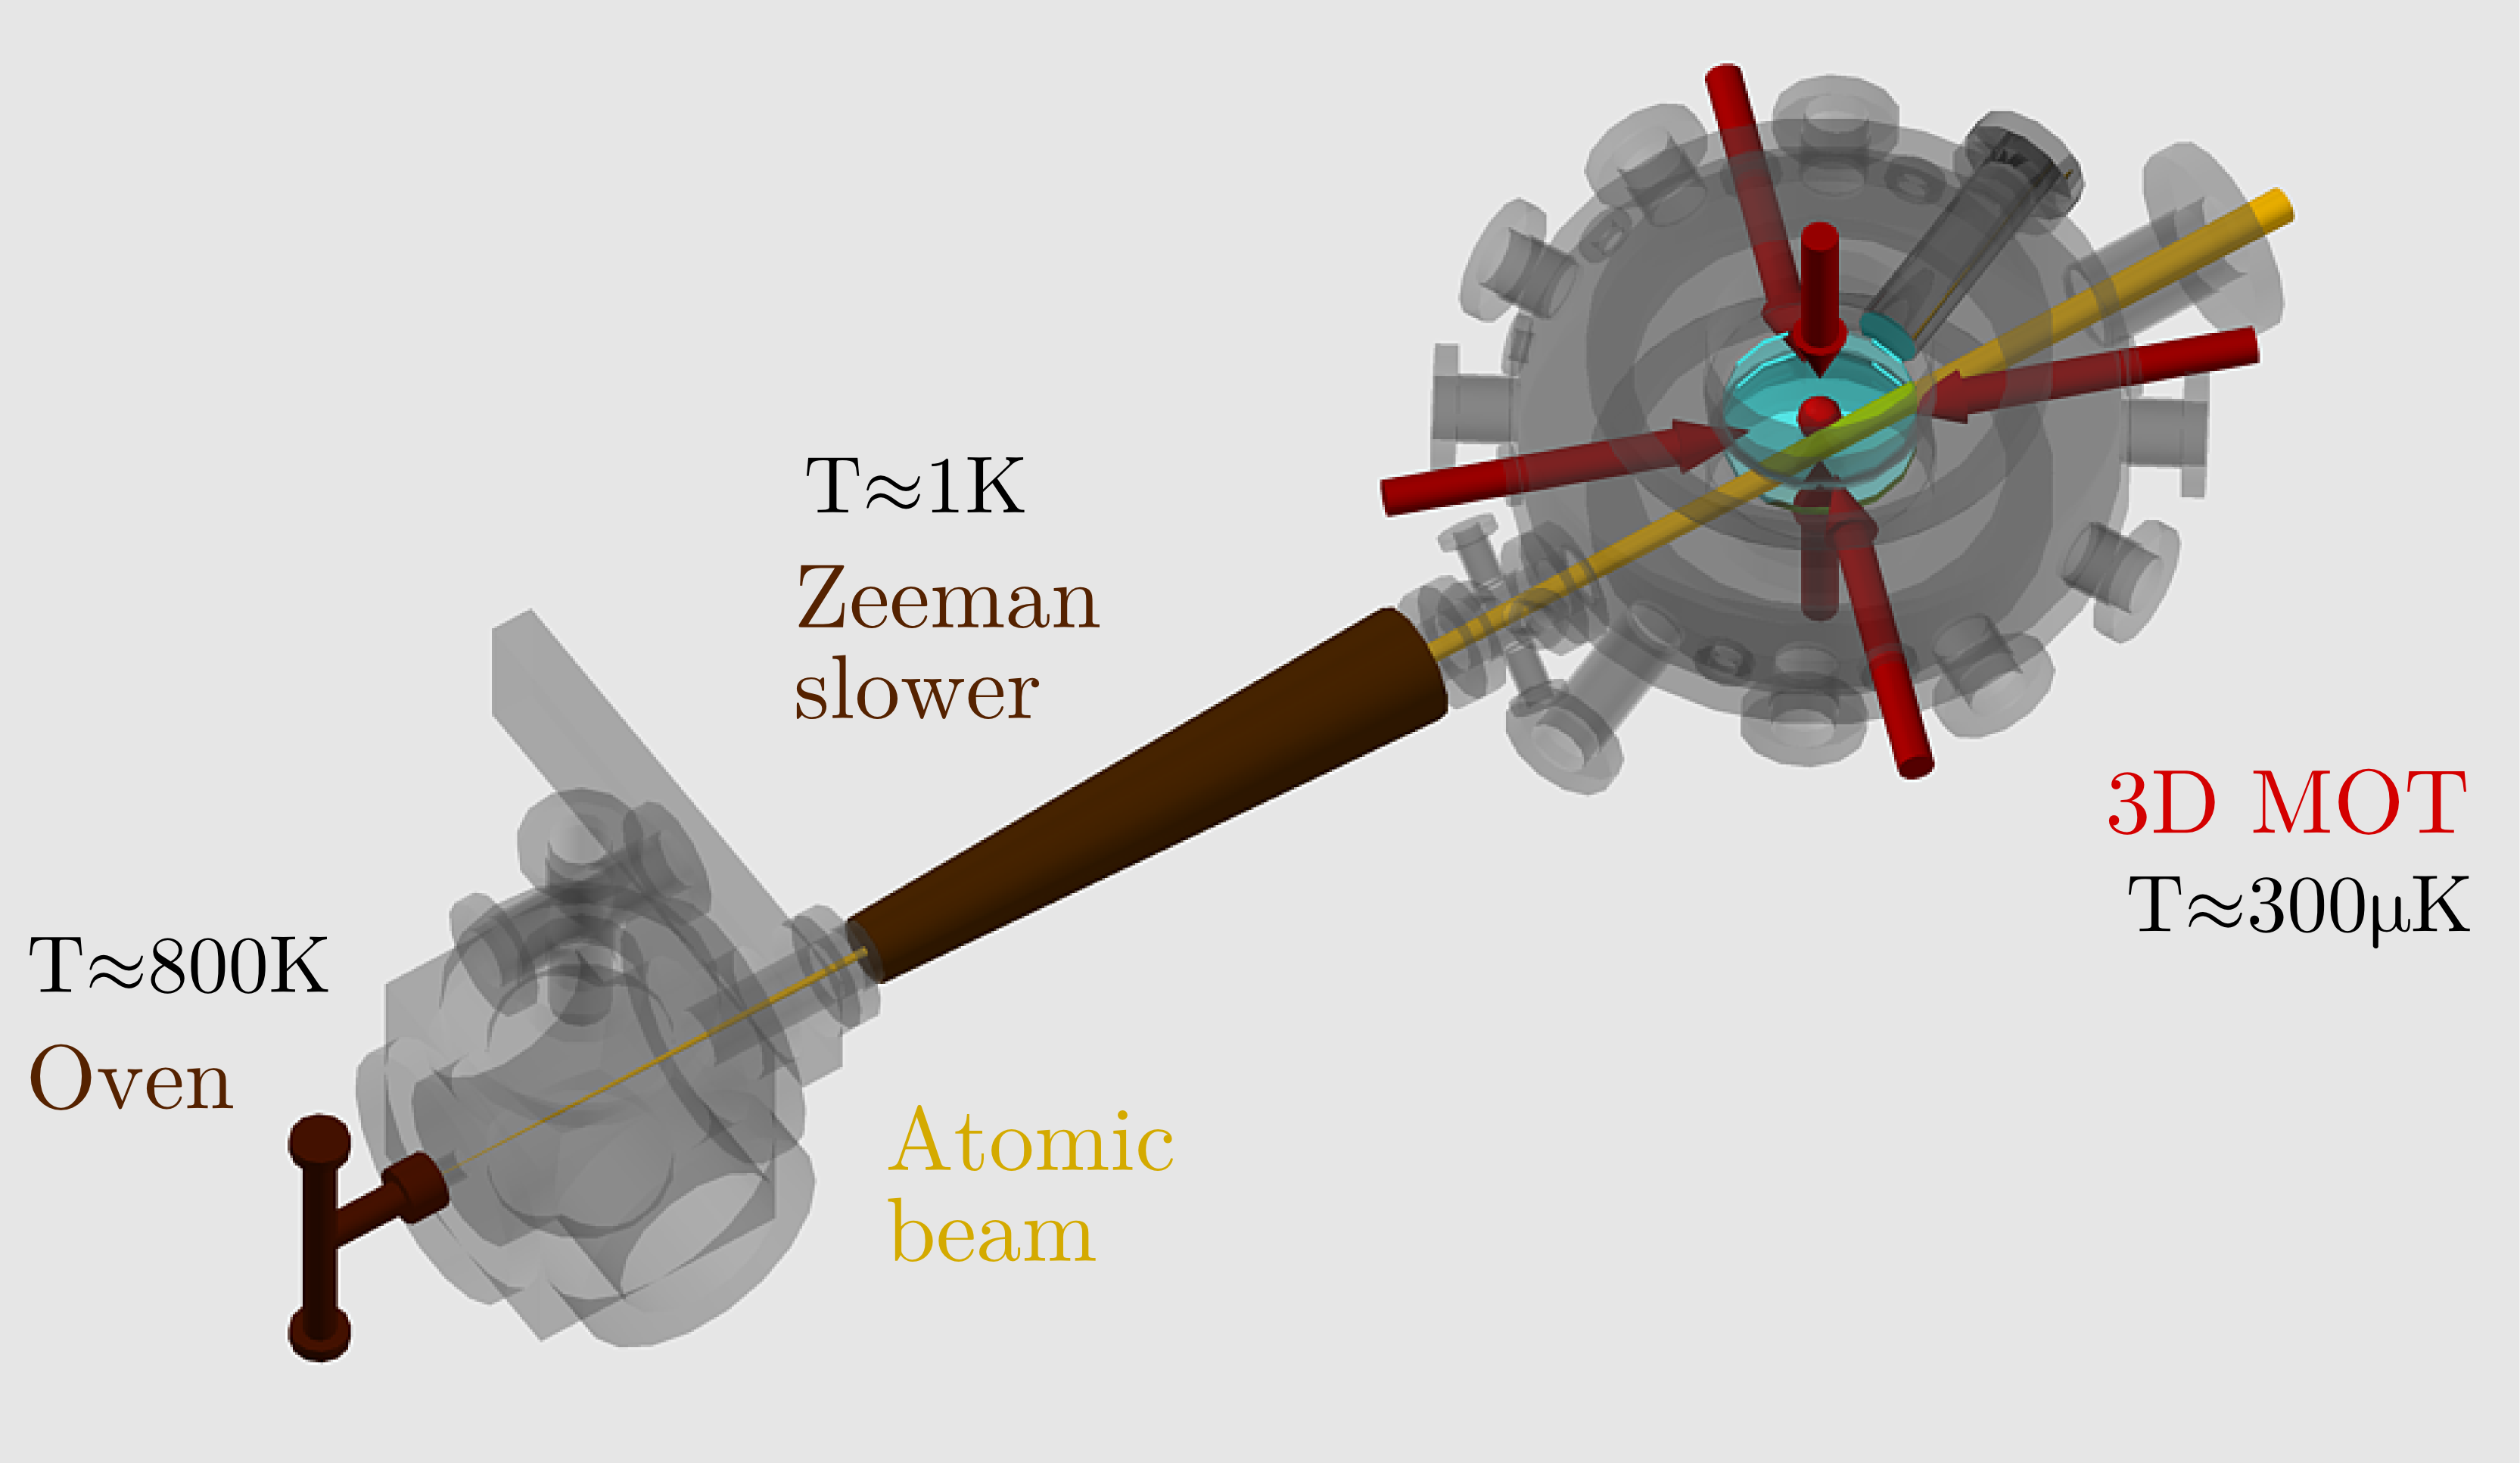
\includegraphics[width=0.8\textwidth]{../masters-figures/apparatus-schem.png}
\caption[Apparatus schematic ]{\small Schematic of apparatus showing the oven,
Zeeman slower and 3DMOT.  The 2DMOT beams (not shown) enter the setup on the
small 4-way cross located between the slower and the main chamber. Notice that
the atomic beam is slightly offset from the center of the chamber. }
\label{fig:apparatus-schem} 
\end{figure} 

In 5~s we load 1.4$\times10^{9}$ atoms in the MOT at a temperature of
$\sim$780~$\mu$K.  After loading, we shutter the Zeeman slower laser using a
hard disk drive shutter~\cite{HardDriveShutter2007}.   At this point we proceed
to cool and compress the 671 nm MOT by  reducing the intensity and detuning of
the the cooling and repumping light, and increasing the magnetic field gradient
to the values shown as CMOT on Table.~\ref{tab:cmot}.
\begin{table}

\centering
\scalebox{1.0}{
\begin{tabular}{l|cc|c}
 &  MOT & CMOT & unit\\
\hline  \hline \noalign{\smallskip}
Trap intensity per beam   & 1.26 & 0.034 & $\isat^{2P}$ \\
Trap detuning   & -33 & -12 & MHz\\
Repump intensity per beam & 0.36 & 0.007 & $\isat^{2P}$ \\
Repump detuning & -25.2 & -17 & MHz\\
$dB_{z}/dz$  & 22.6 & 26.1  & G/cm \\ 
\hline \noalign{\smallskip}
Number & 1.5  & 1 & $10^{9}$\\
$1/e$ radius & 0.22 & 0.18  & cm\\
Peak density  & 2.39 & 3.40 & $10^{10}$cm$^{-3}$\\ 
Temperature & 783 & 288 & $\mu$K\\
Phase space density &  3.9$\times 10^{-7}$ & 2.5$\times 10^{-6}$ & -  
\end{tabular}}
\caption[671 nm MOT cooling and compression]{\small Comparison between the
settings used for loading the 671 nm MOT and the settings after cooling and
compressing (CMOT).   $\isat^{2P}=5.1\,\mathrm{mW/cm^{2}}$ is the saturation
intensity of the 671~nm transition. For cooling and compressing, first the
field gradient is increased in 40 ms, then after a wait of 40 ms the intensity
and detuning of the beams are ramped linearly to their final values in 1 ms.
The phase space density is defined as $n_{0}\lambda_{T}^{3}$ where $n_{0}$ is
the peak density and $\lambda_{T}=\frac{h}{(2\pi m \kb T)^{1/2}}$  is the
thermal de Broglie wavelength. } 
\label{tab:cmot}
\end{table}
 We take time-of-flight images of
the MOT and the CMOT, and infer their temperatures by fitting the cloud sizes
to a ballistic expansion as shown in Fig.~\ref{fig:cmotexp}.   
\begin{figure} \hspace{0.16\textwidth}
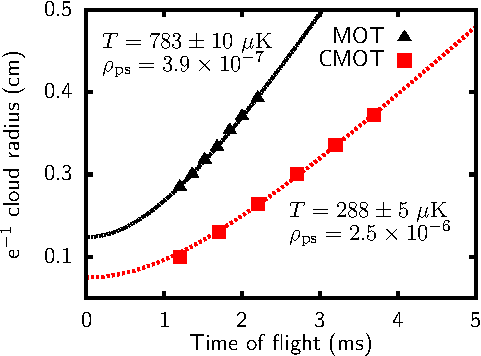
\includegraphics[width=0.58\textwidth]{../masters-figures/323mot/tofexpansion-00/tofeps-SS.pdf}
\caption[671 nm cooled and compressed MOT]{\small  Time-of-flight expansion of
atoms released from the 671 nm MOT right after loading (black triangles) and after
cooling and compressing (red squares). The points represent the $1/e$ width of
Gaussian fits to the spatial profile of the freely expanding clouds.  The lines
are fits to ballistic expansions. $\rho_{\mathrm{ps}}$ stands for phase-space density. } \label{fig:cmotexp} \end{figure}



%########################################
\section{323 nm laser cooling system}
%########################################

Atoms from the 671~nm MOT are transferred to the 323~nm UVMOT, where owing to
the smaller Doppler temperature limit,  lower temperatures can be achieved (see
Fig.~\ref{fig:323levels}).   The Doppler temperature limit, $T_{D}$, of laser
cooling is set by the linewidth of the excited state.  The \uv\ transition
being narrower that the \red\ allows for a lower value of $T_{D}$.  Furthermore
the wavelength of the transition being smaller results in a smaller optical
scattering cross section, which enables reaching larger densities in the UVMOT,
a feature that is favorable when loading the atoms into an optical dipole
trap~\cite{Duarte2011}. 
\begin{figure} \centering
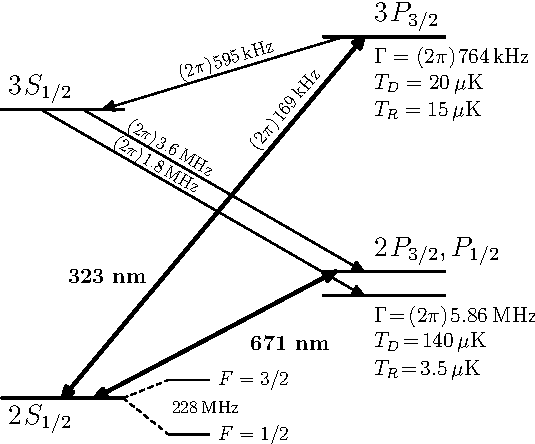
\includegraphics[width=0.65\textwidth]{../masters-figures/levels/323-levels/lithium.pdf}
\caption[Lithium-6 energy level diagram showing the \trep{3/2} state]{\small
Lithium-6 energy level diagram. Lines in bold represent the transitions used to
laser cool atoms. Lighter lines represent decay pathways from the excited
\trep{3/2} state; the decay rates are indicated along the associated paths. On
the right side, beside each excited state we show its linewidth, the associated
Doppler temperature limit ($T_{D}$),  and the recoil temperature limit
($T_{R}$).  }
\label{fig:323levels} \end{figure} 

%----------------------------------------
\subsection{Laser system}
%----------------------------------------

The 323~nm laser system is much simpler than the 671~nm system.  We use a
commercial second harmonic generation (SHG) system from Toptica Photonics to
generate the UV light.  The frequency is stabilized via saturated absorption
spectroscopy, and trapping and repumping frequencies are derived via using
acousto-optic modulators.  The 323~nm system is on the same table as the vacuum
system so we do not use optical fibers,  the light is guided in free space
using mirrors to the final UVMOT configuration.  A schematic of the laser
system is shown in Fig.~\ref{fig:323setupfig}. 
\begin{figure} \centering
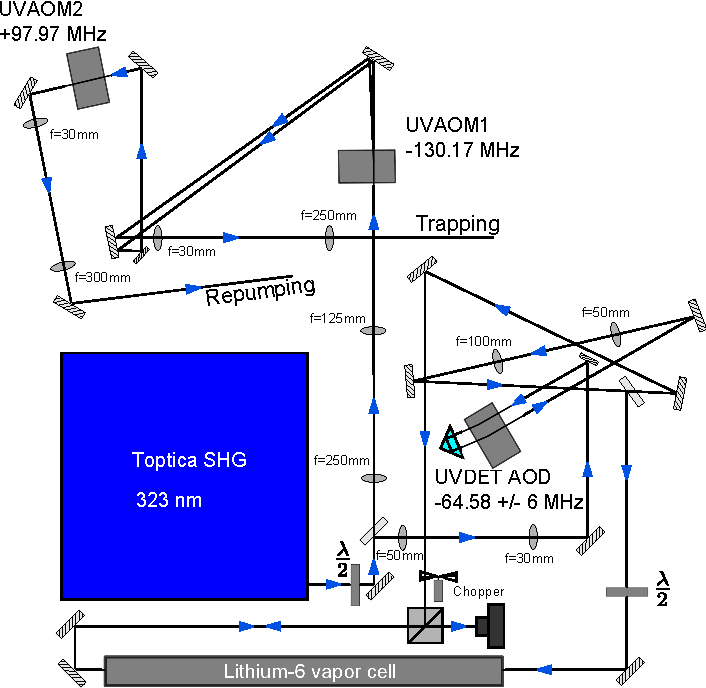
\includegraphics[width=0.7\textwidth]{../masters-figures/323setup/aomsetup/optical_setup.pdf}
\caption[Schematic of modulation transfer spectroscopy]{\small Schematic
showing the optical setup for the 323~nm laser system.   The frequency is
stabilized using a saturated absorption spectroscopy setup~\cite{DuarteMs}.
The light that goes to the experiment is passed through an AOM (labeled
UVAOM1),  the first order is used for trapping and the zeroth order is sent to
a second AOM (labeled UVAOM2) whose first order is used as the repump
frequency.  Trapping and repumping light are combined (not shown) and then
split into six paths for the UVMOT.}
\label{fig:323setupfig}  
\end{figure}


%----------------------------------------
\subsection{UVMOT}
%----------------------------------------

To choose the waist of  the UVMOT beams we had to take into consideration the
available laser power and the transmission losses on the viewports of our
apparatus, which are not anti-reflection coated at
323 nm.  Figure~\ref{fig:012} tabulates the losses at each viewport.
\begin{figure} \begin{minipage}{0.5\linewidth}
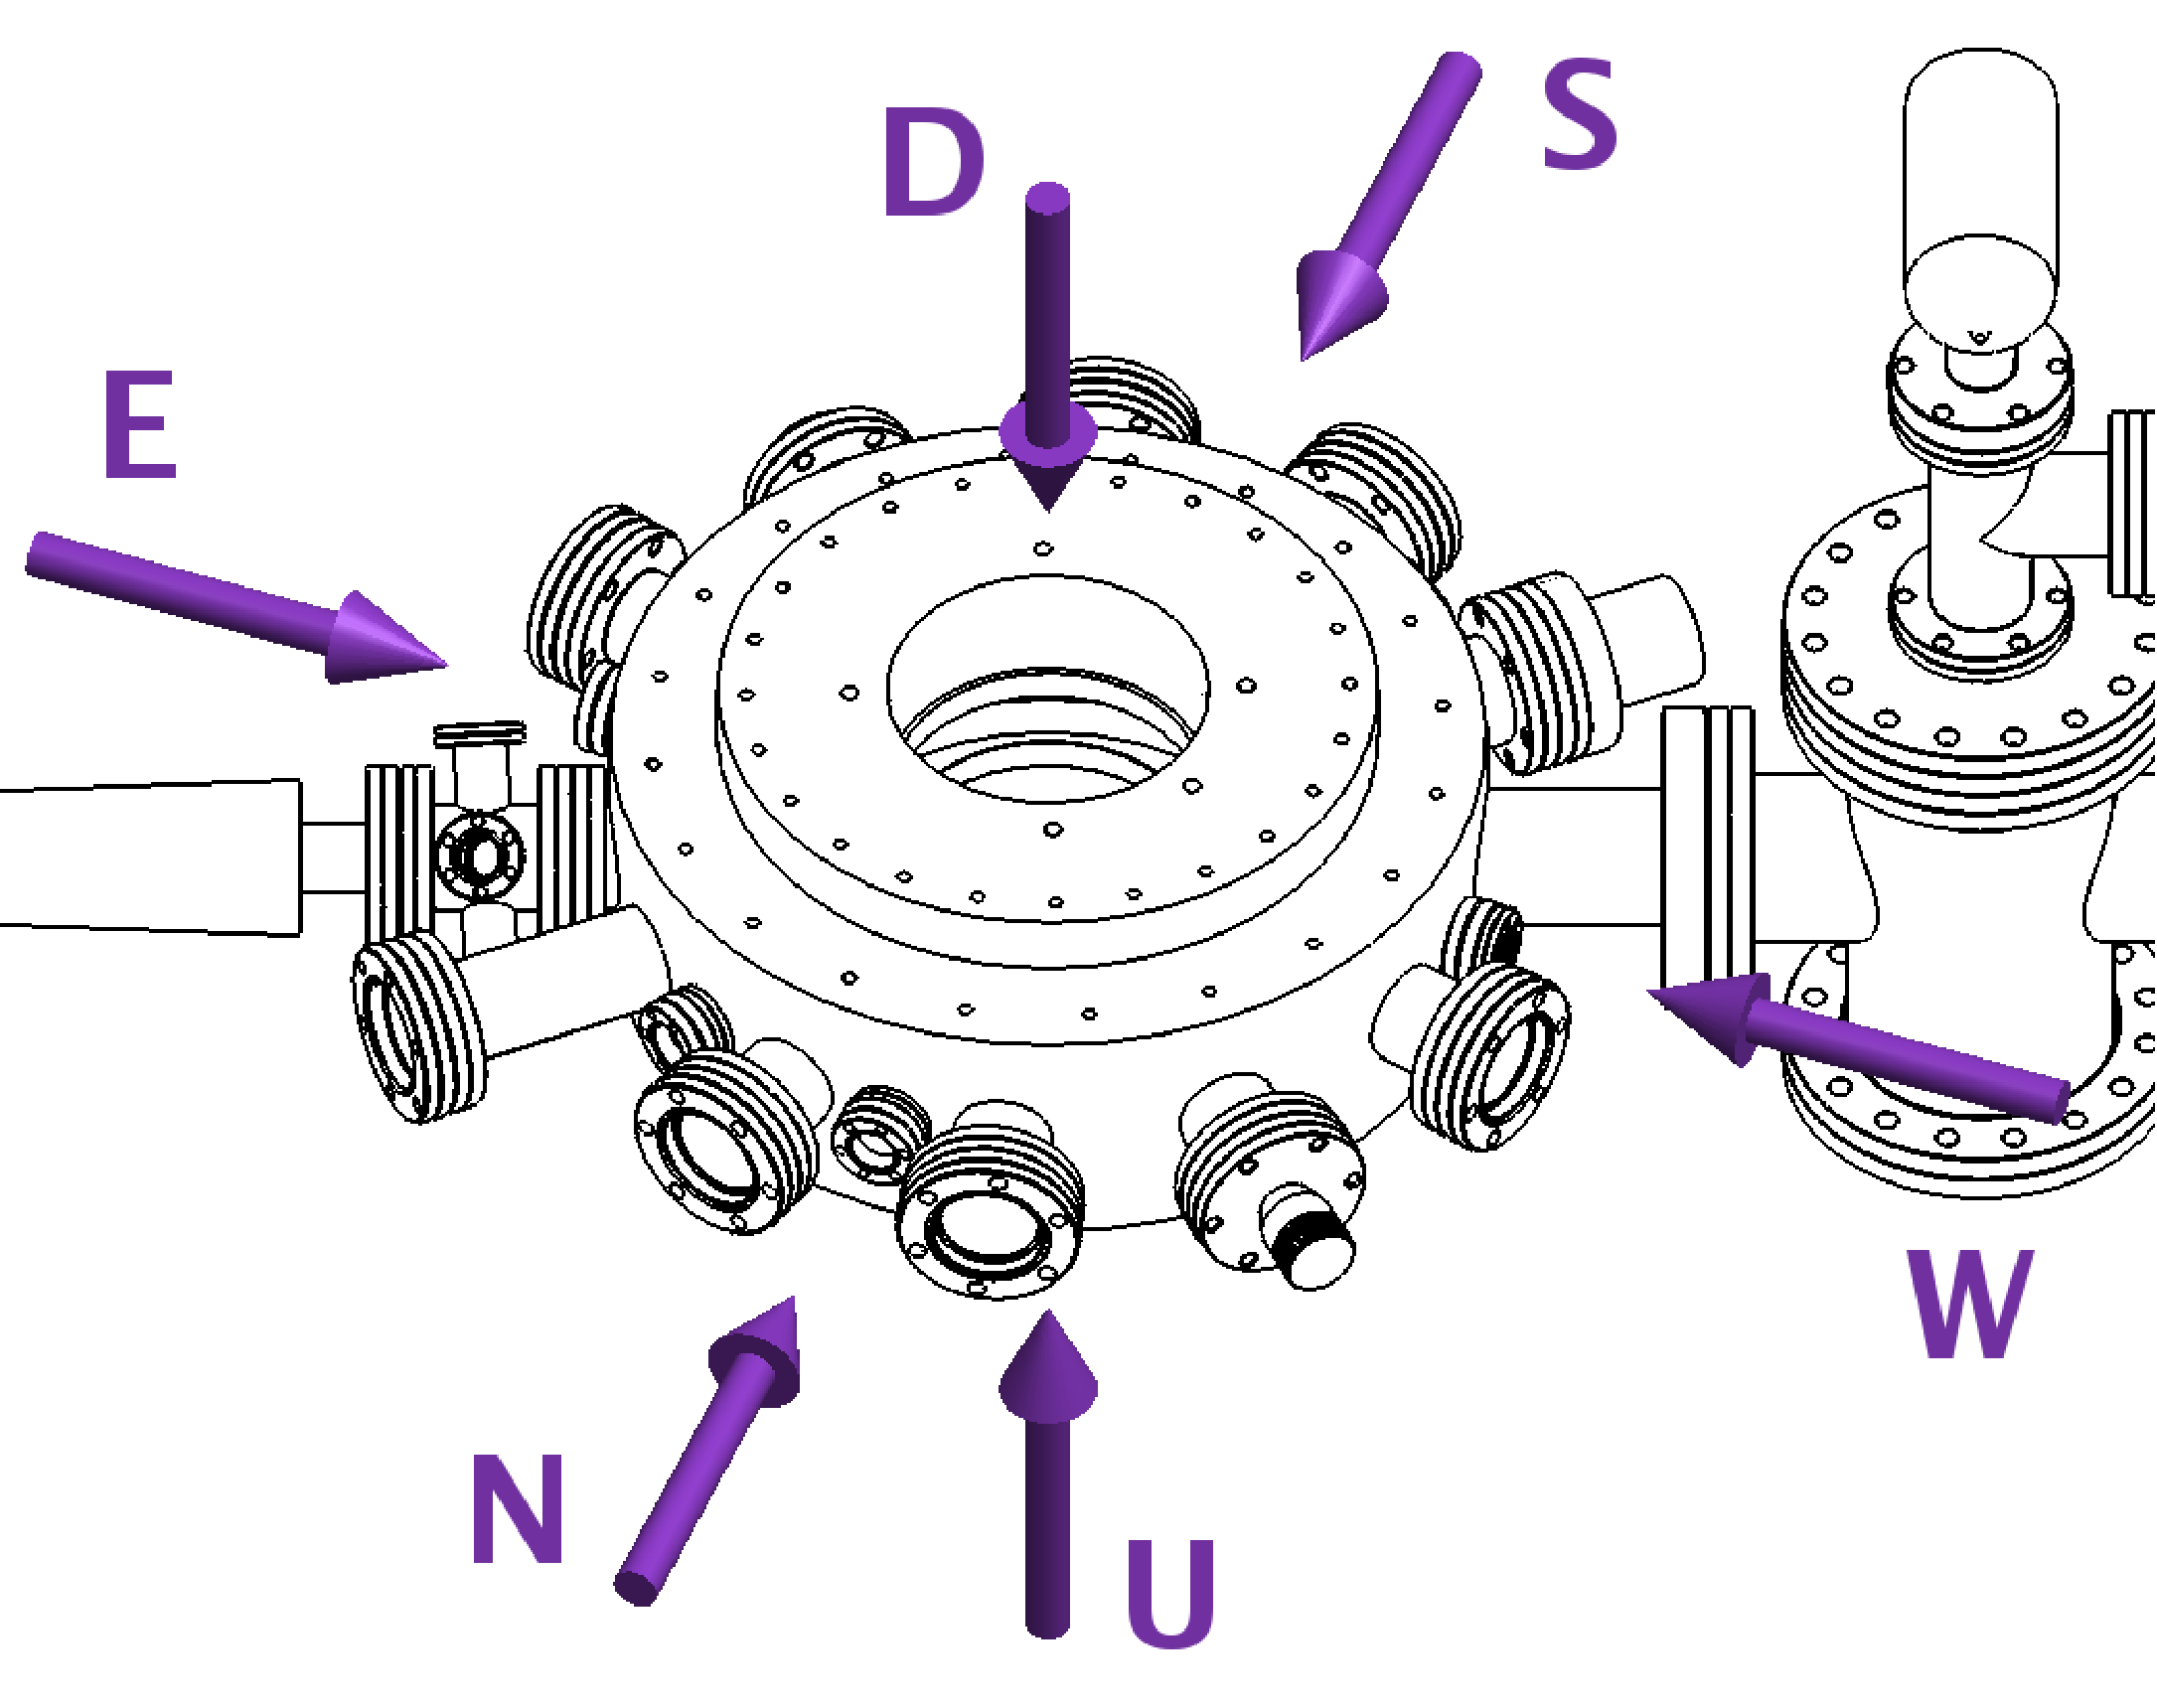
\includegraphics[width=\textwidth]{../masters-figures/323setup/losses/losses.pdf}
\end{minipage} \begin{minipage}{0.5\linewidth} \centering \begin{tabular}{r|c}
& \% Transmission  \\ \hline N & 68 \\ S & 87 \\ E & 75 \\ W & 58 \\ U & 40 \\
D & 40 \\ \end{tabular} \end{minipage} \caption[UVMOT Losses on windows]{\small
This figure shows the percentage transmission of the 323 nm light through the
viewports on our vacuum chamber.  For the side viewports the losses were
accounted for by measuring the power reflected back by the window.  For the top
and bottom viewport it was harder to make this measurement due to restricted
access, so the square root of the transmission through both windows is used. }
\label{fig:012} \end{figure} 
We set up all the beams to have the same intensity at the atoms, thus carefully
taking into account the losses at each window.  This was accomplished by
varying the angle of incidence on dielectric beamsplitters until the desired
power ratios were achieved.  
%Polarization beamsplitter cubes for 323 nm are expensive because they have to
%be optically contacted.  We have observed that the UV light progressively
%damages the cement used in lower priced polarizing beam-splitter cubes.  We
%did keep one polarizing beam-splitter cube (not optically contacted) in our
%setup for doing the first split of the UVMOT beams.  This allows some
%variability in the power balance without having to realign the entire system.
%Currently we loose 14\% of the light on the mentioned cube.  
Considering the losses at the windows and other UV optics, We set the beam waist
of the UVMOT beams to 3.3~mm, which results in an intensity of 1.0$\isat^{3P}$
per beam at an SHG output power of 27.4~mW.  Here $\isat^{3P}=5.9$\,mW/cm$^{2}$
is the saturation intensity of the 323~nm transition.  

The UVMOT uses the same viewports as the 671 nm MOT. All six beams of both
wavelengths are overlapped on dichroic mirrors that transmit 671 nm and reflect
323 nm.  We were lucky to find a long-pass filter (Part Num. NT64-634) from
Edmund Optics that, at very low cost per piece, provides $>99$\% reflection at
323 nm and $>99$\% transmission at 671 nm for both S and P polarizations at a
45$^{\circ}$ angle of incidence.  The UVMOT and red MOT share an axis with the
optical dipole trap (beams $S$ and $N$ on Fig.~\ref{fig:012}).   After the 671
nm and 323 nm are combined, they are overlapped with the optical dipole trap
(1070~nm) or optical lattice (1064~nm) light using a trichroic mirror (Custom
made part from RMI Co.)  that reflects IR and transmits 671~nm and 323~nm.  The
trichroic mirrors have a reflection coefficient  $R>99.5$\% measured at 1064 nm
and 1070 nm, and a transmission coefficient $T=99$\% at 671 nm and $T=90$\% at
323 nm, all measured at a 45$^{\circ}$ angle of incidence.  Also the $U$ and
$D$ beams of the UVMOT share an axis with the optical lattice (1064~nm and
532~nm).  In this case a tetrachroic mirror (Lambda Research Optics) is used to
overlap the wavelengths.  This mirror satisfies $R_{532\,\mathrm{nm}} \approx
0.92$, $R_{1064\,\mathrm{nm}}\approx 0.99$, $T_{671\,\mathrm{nm}}\approx0.92$,
and $T_{323\,\mathrm{nm}}\approx0.86$. 


%----------------------------------------
\subsection{Transfer from MOT to UVMOT}
\label{subsec:mot-uvmot}
%----------------------------------------


The timing diagram for loading the UVMOT from the CMOT is shown
in Fig.~\ref{fig:timingUV}.  The procedure consists of quickly reducing the
magnetic field gradient and turning on the UV light at the same time as the
671~nm light is turned off.  The magnetic field gradient is ramped back up
slowly for compression.  The UV detuning is constant throughout.  The
operating values of the UVMOT are shown in Table~\ref{tab:uvmotUV}, and a
measurement of the temperature is shown in Fig.~\ref{fig:uvtexpUV}. 

\begin{figure} \centering
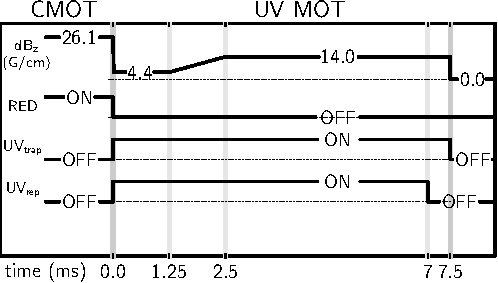
\includegraphics[width=0.5\textwidth]{../masters-figures/323mot/timingdiagram-nodet/timing.pdf}
\caption[UVMOT loading timing diagram]{\small Timing diagram representing the
transfer sequence from the CMOT to the UVMOT. } \label{fig:timingUV}
\end{figure}

\begin{table} \centering 
\scalebox{1.0}{
\begin{tabular}{l|c|c} 
&  UVMOT  & unit\\ 
\hline  \hline \noalign{\smallskip} 
$dB_{z}$ Final & 14 & G/cm \\ 
\hline \noalign{\smallskip}
SHG Output power &  25 & mW \\
UV trap intensity per beam & 1.0 & $\isat^{3P}$ \\
UV repump intensity per beam & 0.1 & $\isat^{3P}$ \\
UV detuning (UVMOT only) & -1.6 & MHz \\
UV detuning (loading to ODT) & -0.6 & MHz \\
\hline \noalign{\smallskip} 
Number & 5.3 & $10^{8}$  \\ 
$1/e$ radius & 0.15  & cm \\ 
Peak density & 2.9  & $10^{10}$\,cm$^{-3}$ \\ 
Temperature & 59 & $\mu$K \\ 
Phase space density &  2.3$\times 10^{-5}$ & - 
\end{tabular}}
\caption[UVMOT settings]{\small UVMOT Settings.
$\isat^{3P}=5.9\,\mathrm{mW/cm^{2}}$ is the saturation intensity of the 323~nm
transition.~\cite{Duarte2011}. The two values shown for the detuning correspond
to optimized number and temperature of the UVMOT (Fig.~\ref{fig:uvtexpUV}), and
optimized number of atoms loaded into the ODT.  More details on loading the ODT
will be given on \S\ref{sec:odtload}. }
\label{tab:uvmotUV} \end{table}

\begin{figure}
\hspace{0.16\textwidth}
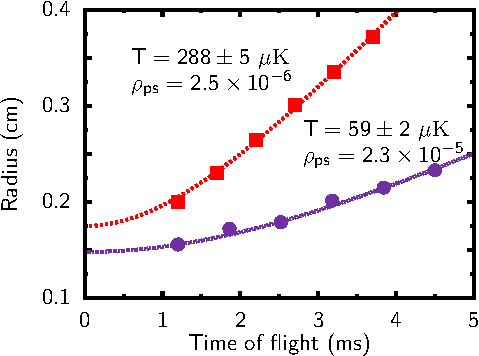
\includegraphics[width=0.58\textwidth]{../masters-figures/323mot/tofexpansion/tofeps.pdf}
\caption[CMOT and UVMOT time-of-flight expansion]{\small Time-of-flight
expansion of the CMOT (red squares) and the UVMOT  (violet circles).  The
points represent the $1/e$ width of Gaussian fits to the spatial profile of the
freely expanding clouds.  The lines are fit to ballistic expansions.
$\rho_{\mathrm{ps}}$ stands for phase-space density.}
\label{fig:uvtexpUV} \end{figure} 



%########################################
\section{Optical dipole trap}
%########################################

We load the atoms from the UVMOT into the optical dipole trap (ODT), where we
evaporatively cool them to degeneracy. The light for the ODT is provided by a
broadband fiber laser operating at 1070~nm with an output power of 50~W.  Two
beams with orthogonal polarizations cross at an angle of 15$^{\circ}$ to form a
crossed-beam trap. The resulting potential resembles an elongated ellipsoid, as
shown in Fig.~\ref{fig:odt-cartoon}. 
\begin{figure} \centering
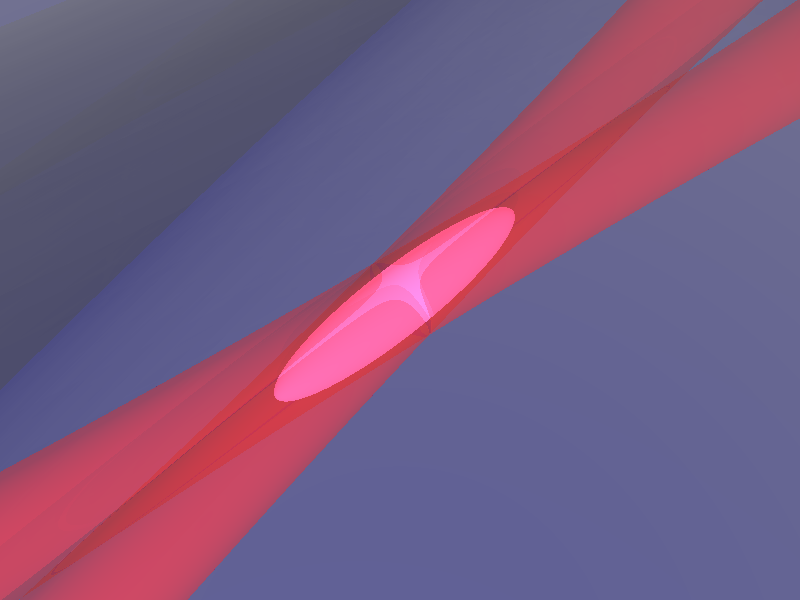
\includegraphics[width=0.4\textwidth]{../masters-figures/odt/15deg-crossbeam.png}
\caption[Optical dipole trap]{\small Illustration of the potential created by
the crossed-beam optical dipole trap.  } \label{fig:odt-cartoon}
\end{figure}

The ODT beams are cylindrically symmetric and focused to a waist of
$\sim70~\mu$m.  For the purposes of tuning the potential to optimize the number
of atoms loaded, the lens labeled $F$ in Fig.~\ref{fig:odtsetup} is positioned
on a translation stage.  Moving this lens along the beam path has a strong
handle on the waist of the ODT beams, and thus affects the depth and volume of
the trap strongly.  
\begin{figure} \centering
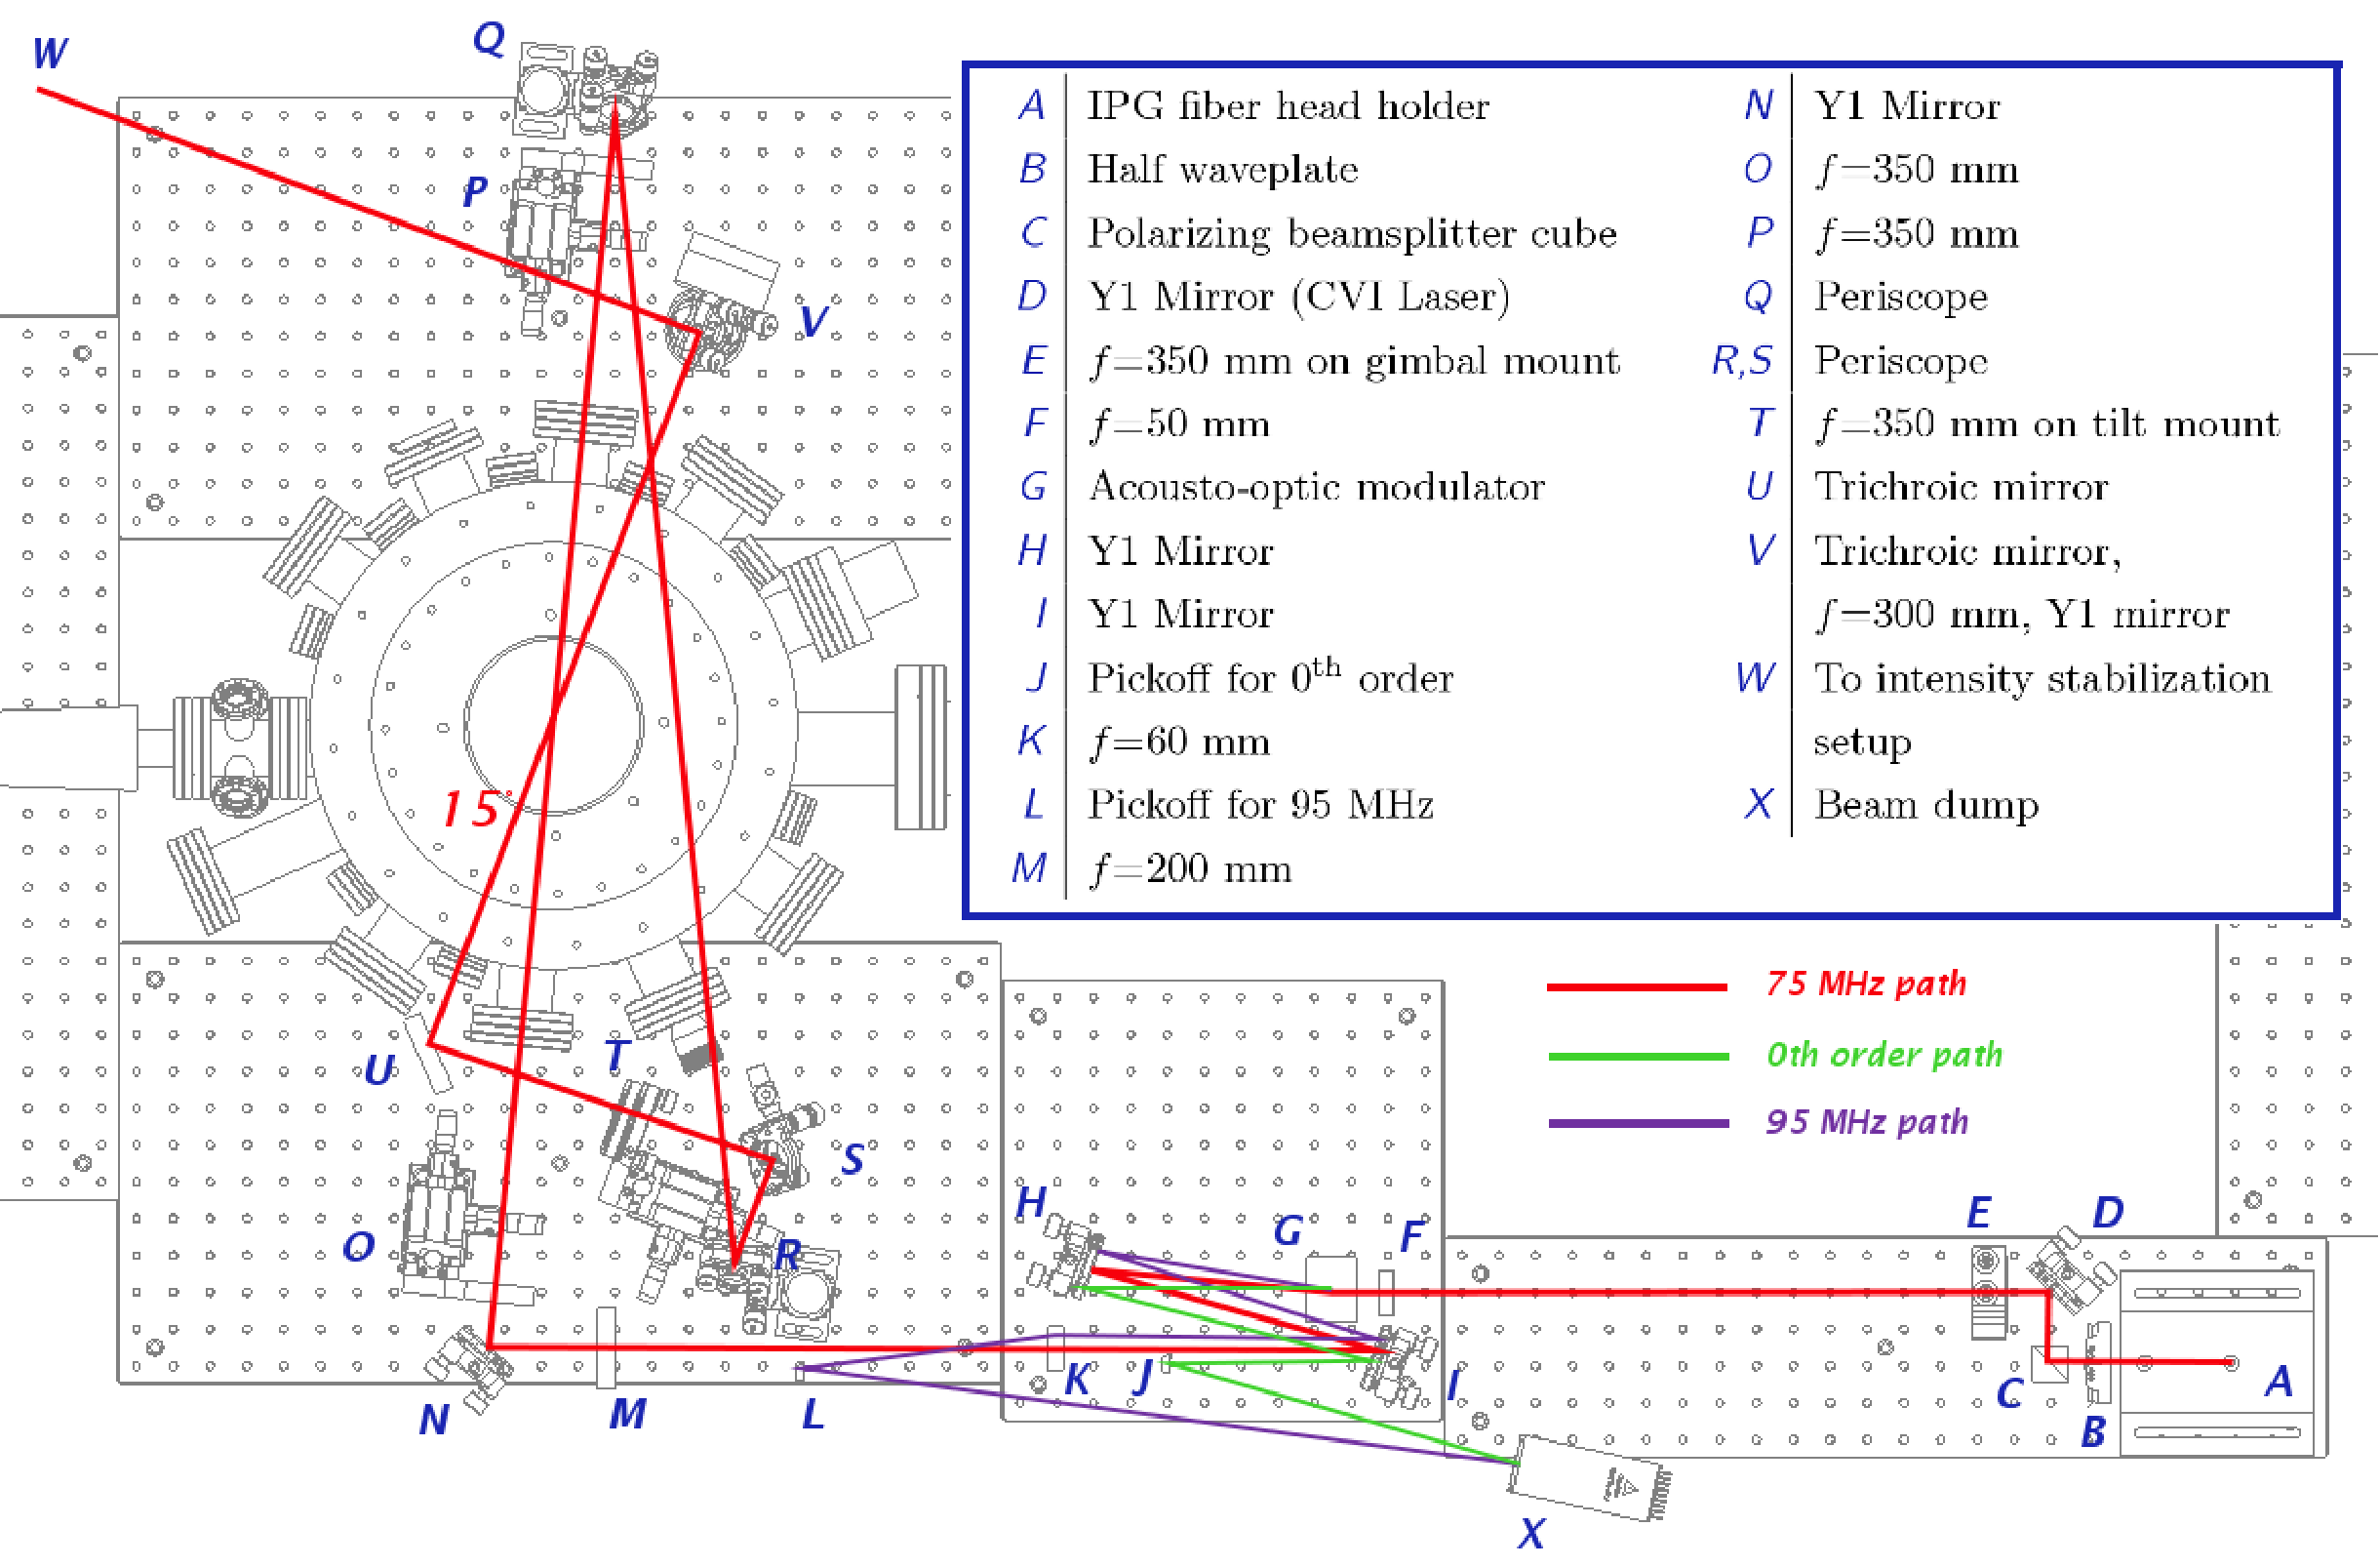
\includegraphics[width=\textwidth]{../masters-figures/odt/opticalsetup/setup.pdf}
\caption[Optical dipole trap setup]{\small Optical dipole trap setup.  The red
lines show the path of the first order of the AOM labeled $G$ when the AOM is
operated at 75~MHz.   Light can be dumped by driving the AOM at 95~MHZ (purple
path) or by turning it off (green path). All mirrors in this setup are Part
Num. Y1-1025-45-UNP from CVI Laser, which have a damage threshold of
10~MW/cm$^{2}$.  All the lens substrates are UV fused silica to reduce power
dissipation and thermal lensing.  The acousto-optic modulator is Part Num.
46080-2-1.06 from Neos Technologies.  } \label{fig:odtsetup}
\end{figure}

\subsubsection{Trap depth and frequencies}

The trapping potential produced by a light field of spatially varying intensity
$I(\bv{r})$ is given by
\begin{equation}
 U_{\mathrm{dip}}(\mathrm{\mathbf{r}} ) =
\frac{\hbar \Gamma^{2}}{4} \left( \frac{1}{\omega_{0}+\omega} +
\frac{1}{\omega_{0}-\omega} \right) \frac{I(\mathrm{\mathbf{r}} )}{\isat} 
\end{equation}
For \li\!\!, a single Gaussian beam of power $P$ and
beam waist $w$, produces a trap depth 
\begin{equation} 
  \frac{U_{0}}{\kb}=\frac{P}{w^{2}} \times
  38.7\times10^{3}  \mu\mathrm{K}\, \mu \mathrm{m}^{2}\, \mathrm{W}^{-1} 
\end{equation}


The first pass through the atoms has 39~W of power and, after losses at
subsequent optics and windows, there are 35~W for the second pass.  The pass
with lower power sets the trap depth,  which is $U_{0}/\kb\approx 280\,\mu$K.  Atoms with an energy higher than $U_{0}$ can escape the intersection
region of the two beams by drifting away along the 39~W beam. 

The trap frequencies are calculated to be approximately 490~Hz and 3750~Hz
along the axial and radial directions of the trap, respectively.  We measured
the radial trap frequency, $\omega_{\mathrm{r}}$, by turning the dipole trap
off briefly (40 $\mu$s) and then turning it back on. The resulting breathing
mode oscillates at twice the radial trap frequency and we obtain
$\omega_{\mathrm{r}} = (2\pi)3.8$~kHz.   The axial trap frequency,
$\omega_{\mathrm{a}}$,  was measured via parametric heating by sinusoidally
modulating the trap depth, and determined to be $\omega_{\mathrm{a}} =
(2\pi)470$~Hz.  



%########################################
\section{Magnetic field}
%########################################

The magnetic field in our experiment is created by a set of coils in
Helmholtz configuration, which sit close to the atoms, inside the recessed top
and bottom viewports of our vacuum chamber (see Fig.~\ref{fig:coilforms}).
\begin{figure} 
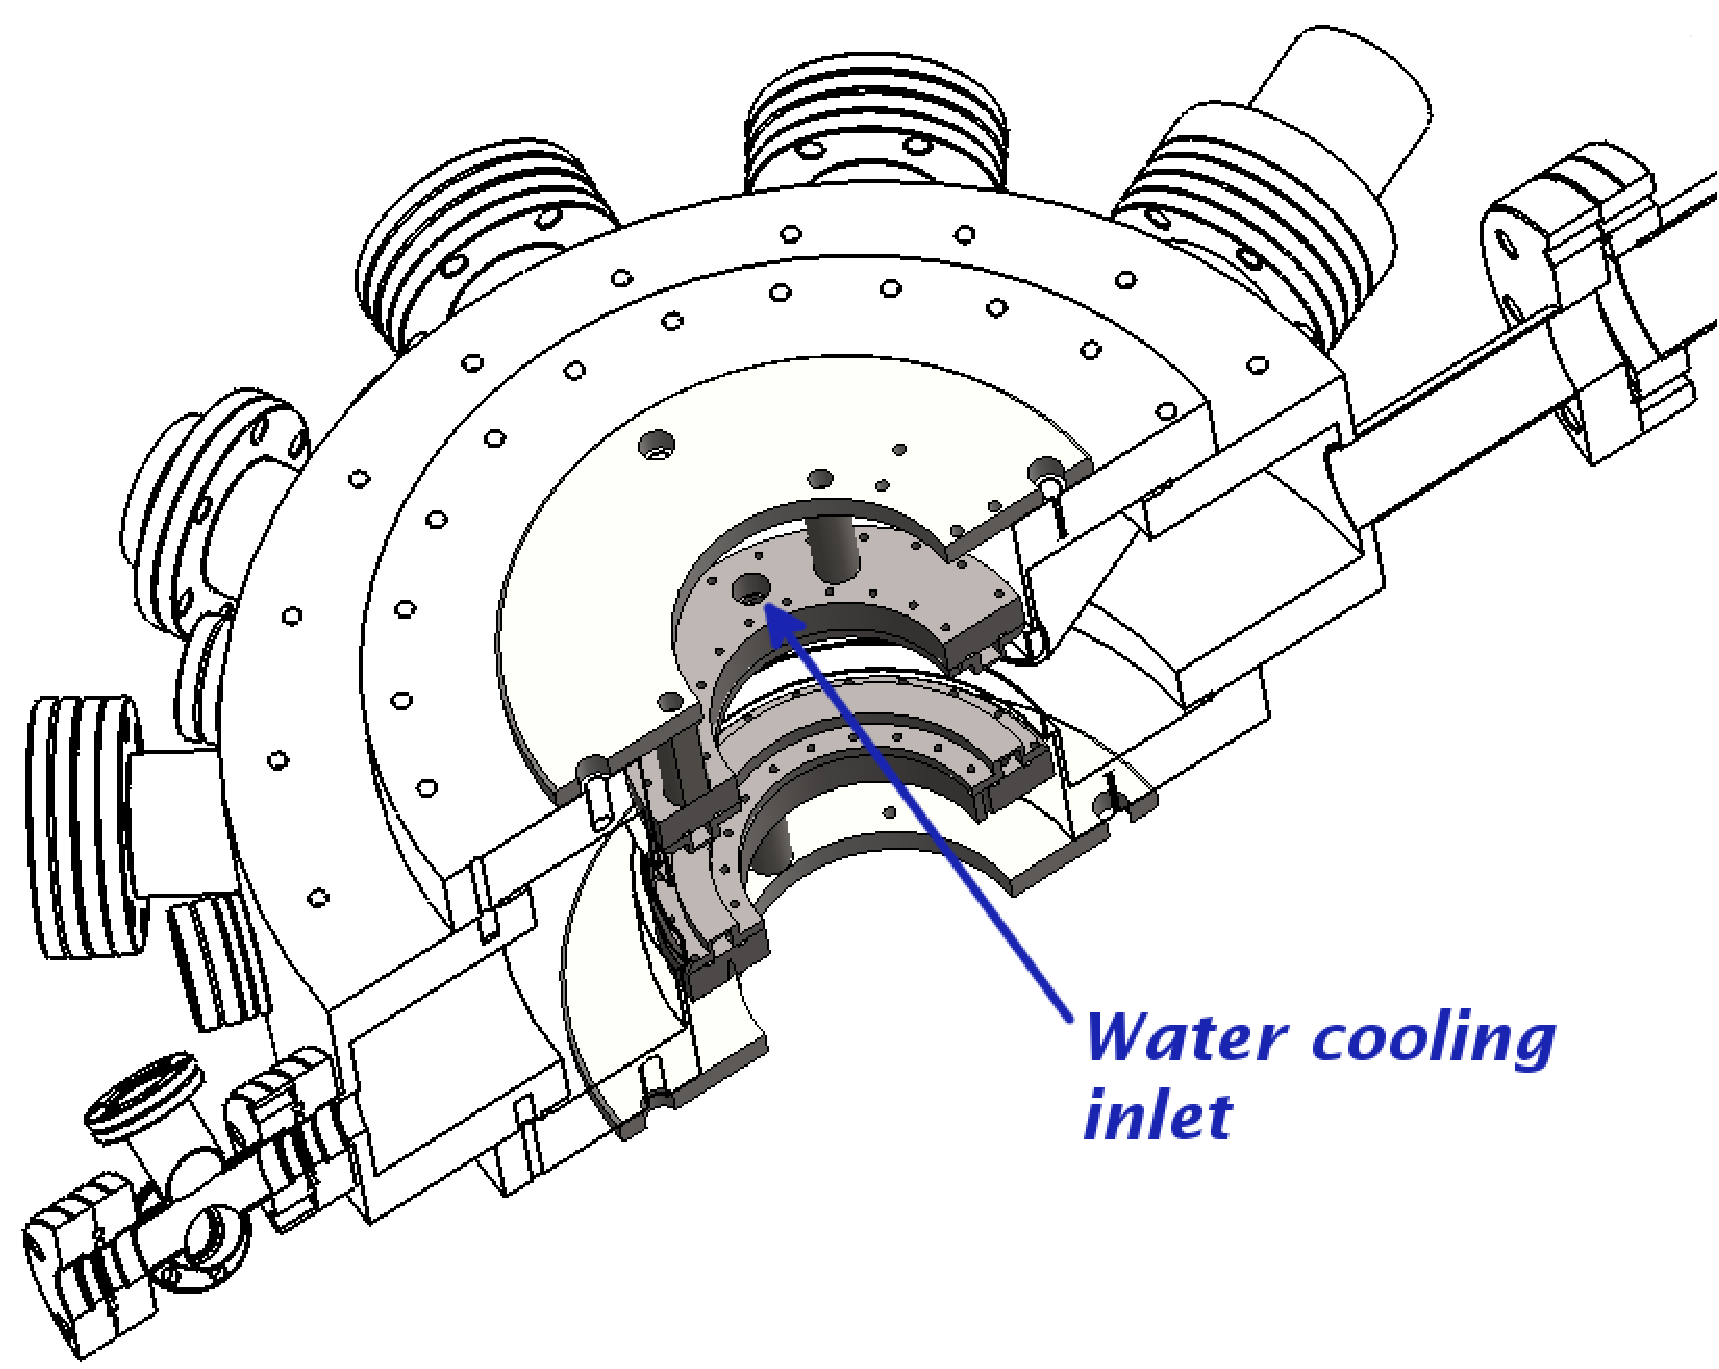
\includegraphics[width=0.45\textwidth]{../masters-figures/coils/angleview.pdf}
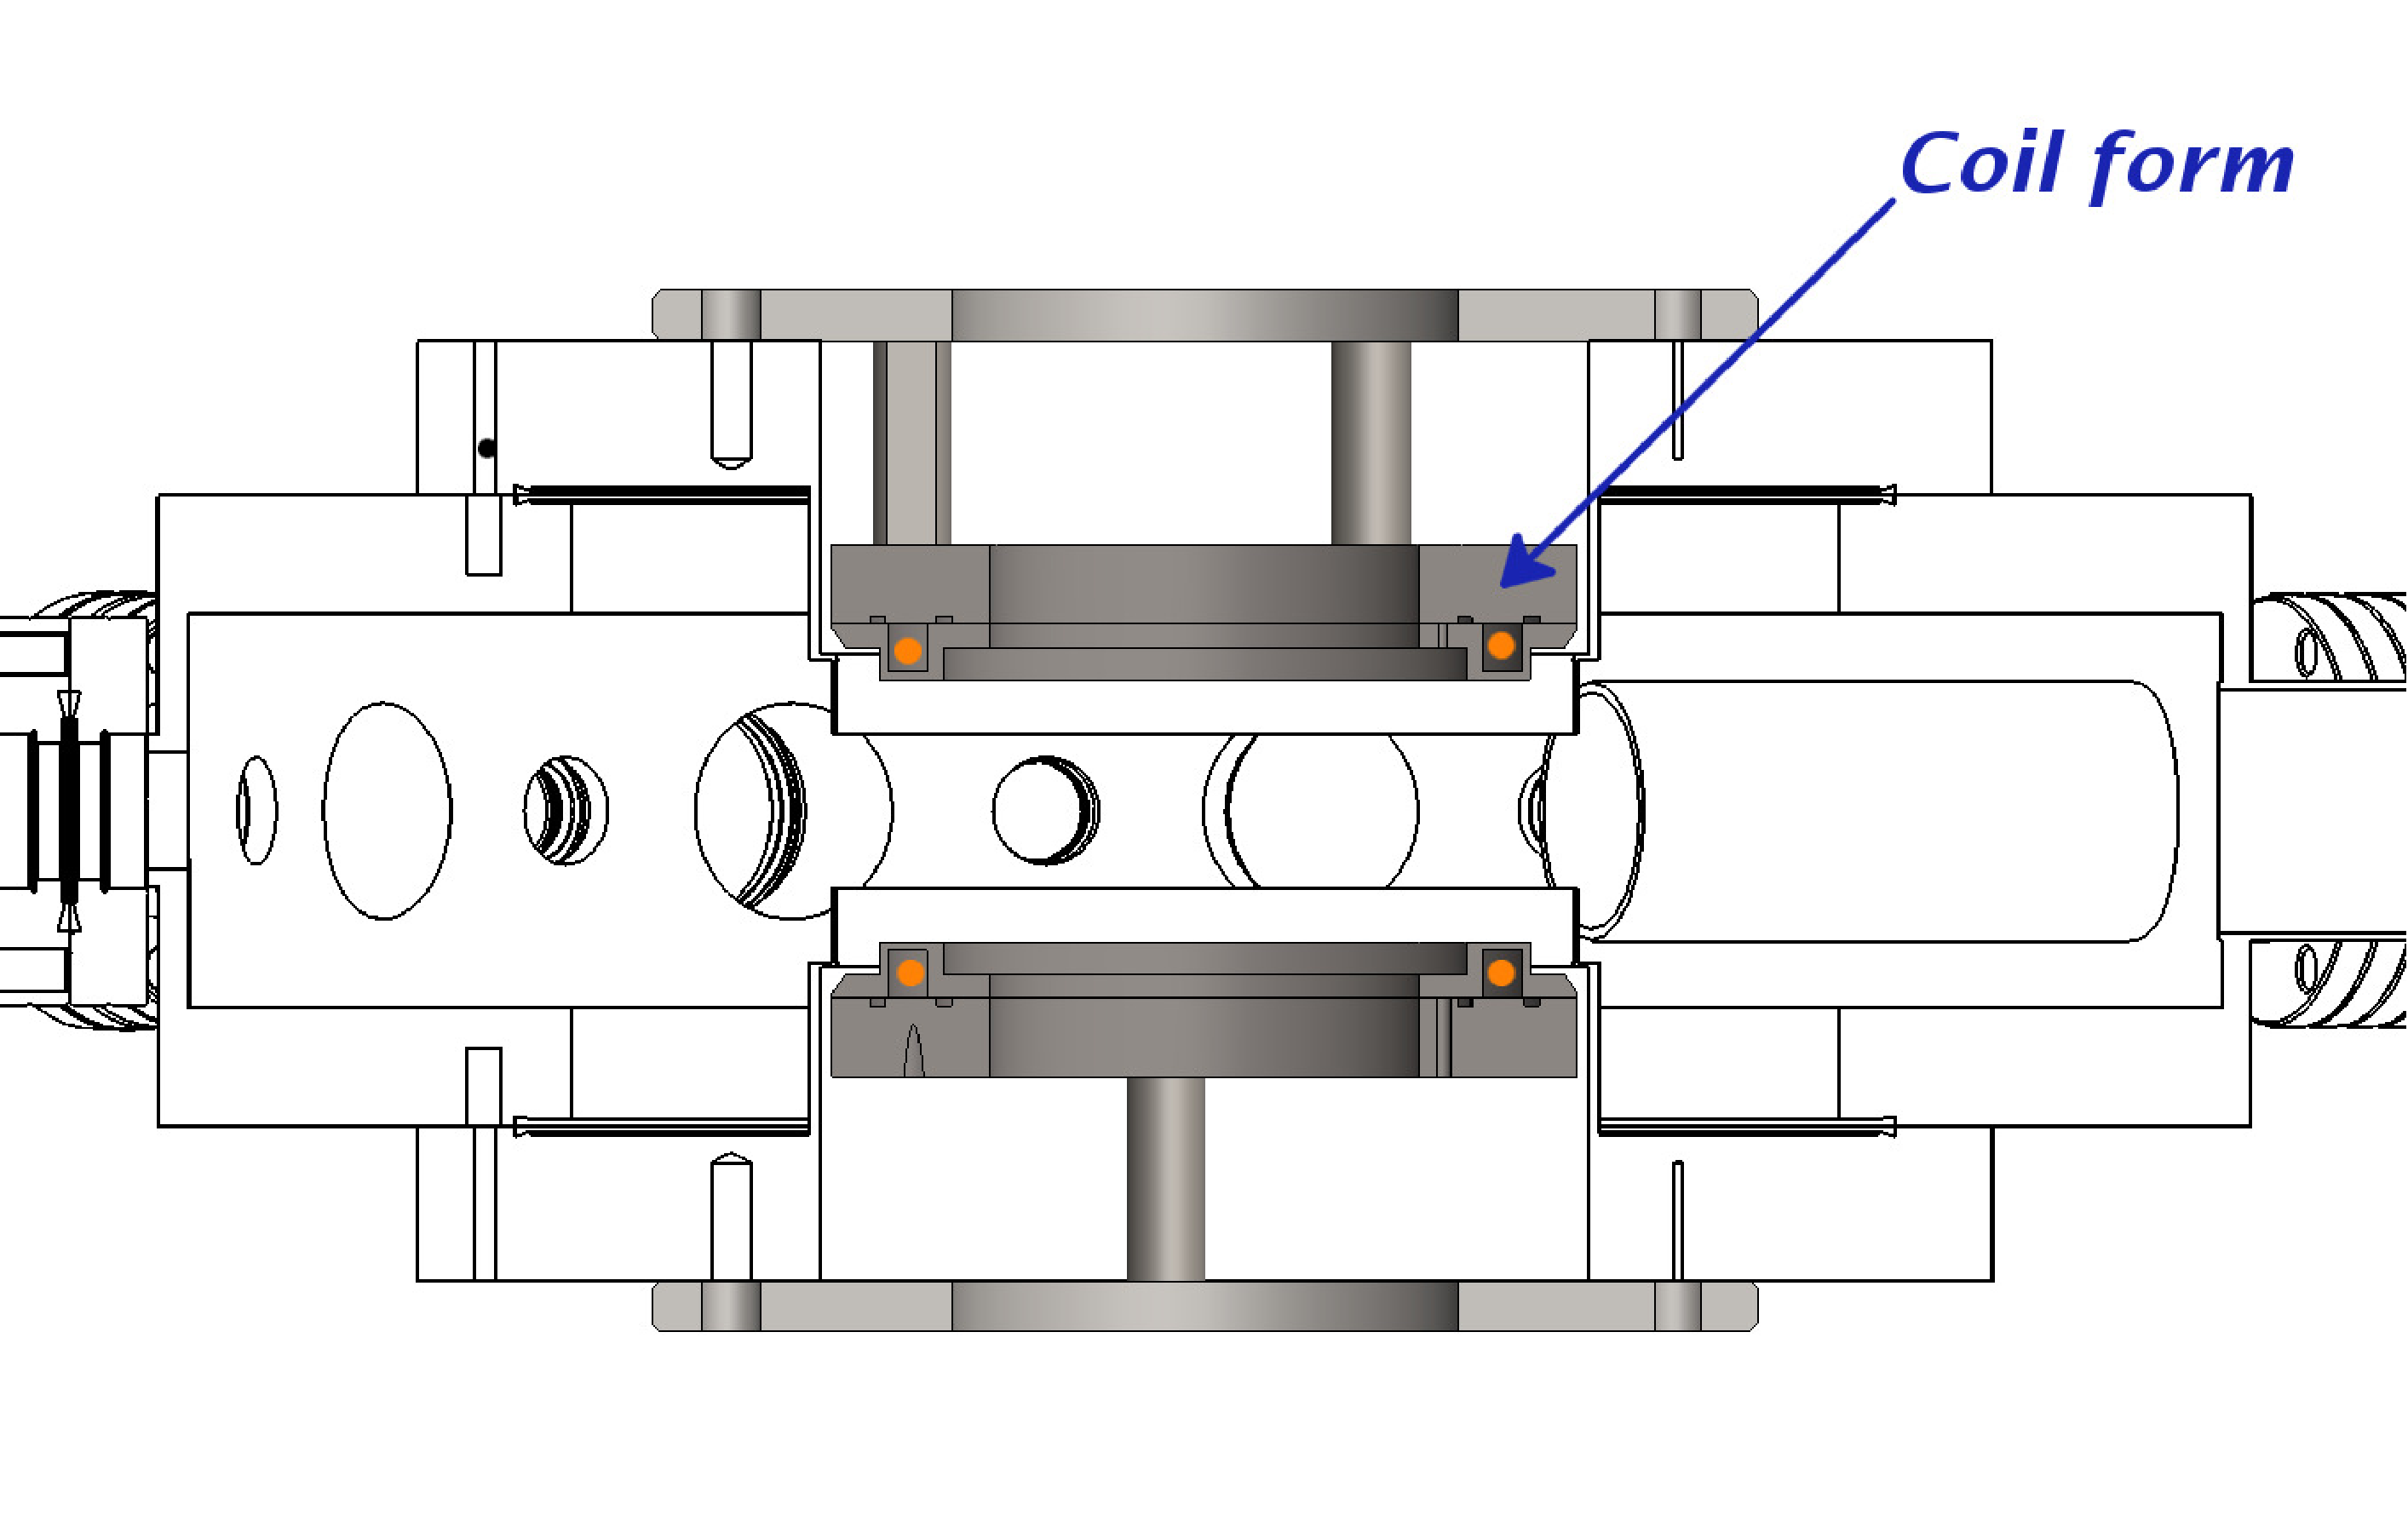
\includegraphics[width=0.55\textwidth]{../masters-figures/coils/sideview.pdf}
\caption[Location of magnetic field coil forms ]{\small Cut-out view of vacuum
chamber showing the location of the coils that create the magnetic field.   The
coil forms are close to the atoms inside the re-entrant top and bottom
viewports.  The forms themselves are attached to a mounting plate that bolts to
the re-entrant viewport flange.  The coils are water cooled.  Only  the water
inlet is shown in this picture, the water outlet is on the half that is cut
out. }
\label{fig:coilforms} 
\end{figure} 
The radius of the coils is 4.72~cm, and is equal to the separation between
them.  There are $n=35$ turns on the top coil and $n-1=34$ turns on the bottom
coil.  As we will see, we take advantage of the mismatch in the number of turns
to levitate the atoms in the latter stages of the experiment.  During the MOT
stages of our experiment, the current through the coils is run such that they
are in anti-Helmholtz configuration. For a current $I$,  the coils produce a
quadrupole magnetic field with a gradient along $z$, given by 
\begin{equation}
 \frac{ \mathrm{d}B_{z}}{ \mathrm{d}z}= \left(
\frac{4}{5} \right) ^{5/2} \frac{3}{4} \frac{\mu_{0} (2n-1) I } { r^{2} } 
\end{equation}
which for $n=35$ and $r=4.72$~cm amounts to 1.72 G/cm/A.

After the optical dipole trap is loaded from the UVMOT the direction of the
current in the top coil is reversed and they produce a bias field given by 
\begin{equation}
 B = \left( \frac{4}{5} \right) ^{3/2} \frac{\mu_{0} (2n-1) I }{2r}  
\end{equation}
 which amounts to  6.8 G/A.   Due to the mismatch in the number of turns
between the two coils, in bias configuration there is a residual gradient given
by 
\begin{equation}
 \frac{ \mathrm{d}B_{z}}{ \mathrm{d}z}= \left(
\frac{4}{5} \right) ^{5/2} \frac{3}{4} \frac{\mu_{0} I } { r^{2} } 
\end{equation}
Fora a bias field of $500-650$~G, where we perform most of our experiments,
this field gradient produces a force on the atoms which is directed upwards and
has about twice the magnitude of the gravitational force.   We have set up
circuitry to controllably shunt some current from the top coil, such that the
atoms are levitated.  
%This is critical for some of our measurements in the
%compensated lattice potential (described in
%Chapter~\ref{chap:compensated-optical-lattice}), where the trapping frequencies
%can be very low.  

The diagram in Fig.~\ref{fig:fieldcircuit} shows a schematic of the magnetic
field system.  The polarity of the current on the top coil is switched by using
an H-bridge made with four field-effect transistors (FETs), labeled $1$ to $4$ in
Fig.~\ref{fig:fieldcircuit}.   FETs labeled 5 and 6 control the amount of
current shunted from the top coil to levitate the atoms.  FETs labeled 7 and 8
control the total amount of current in the system.  
\begin{figure} 
\centering
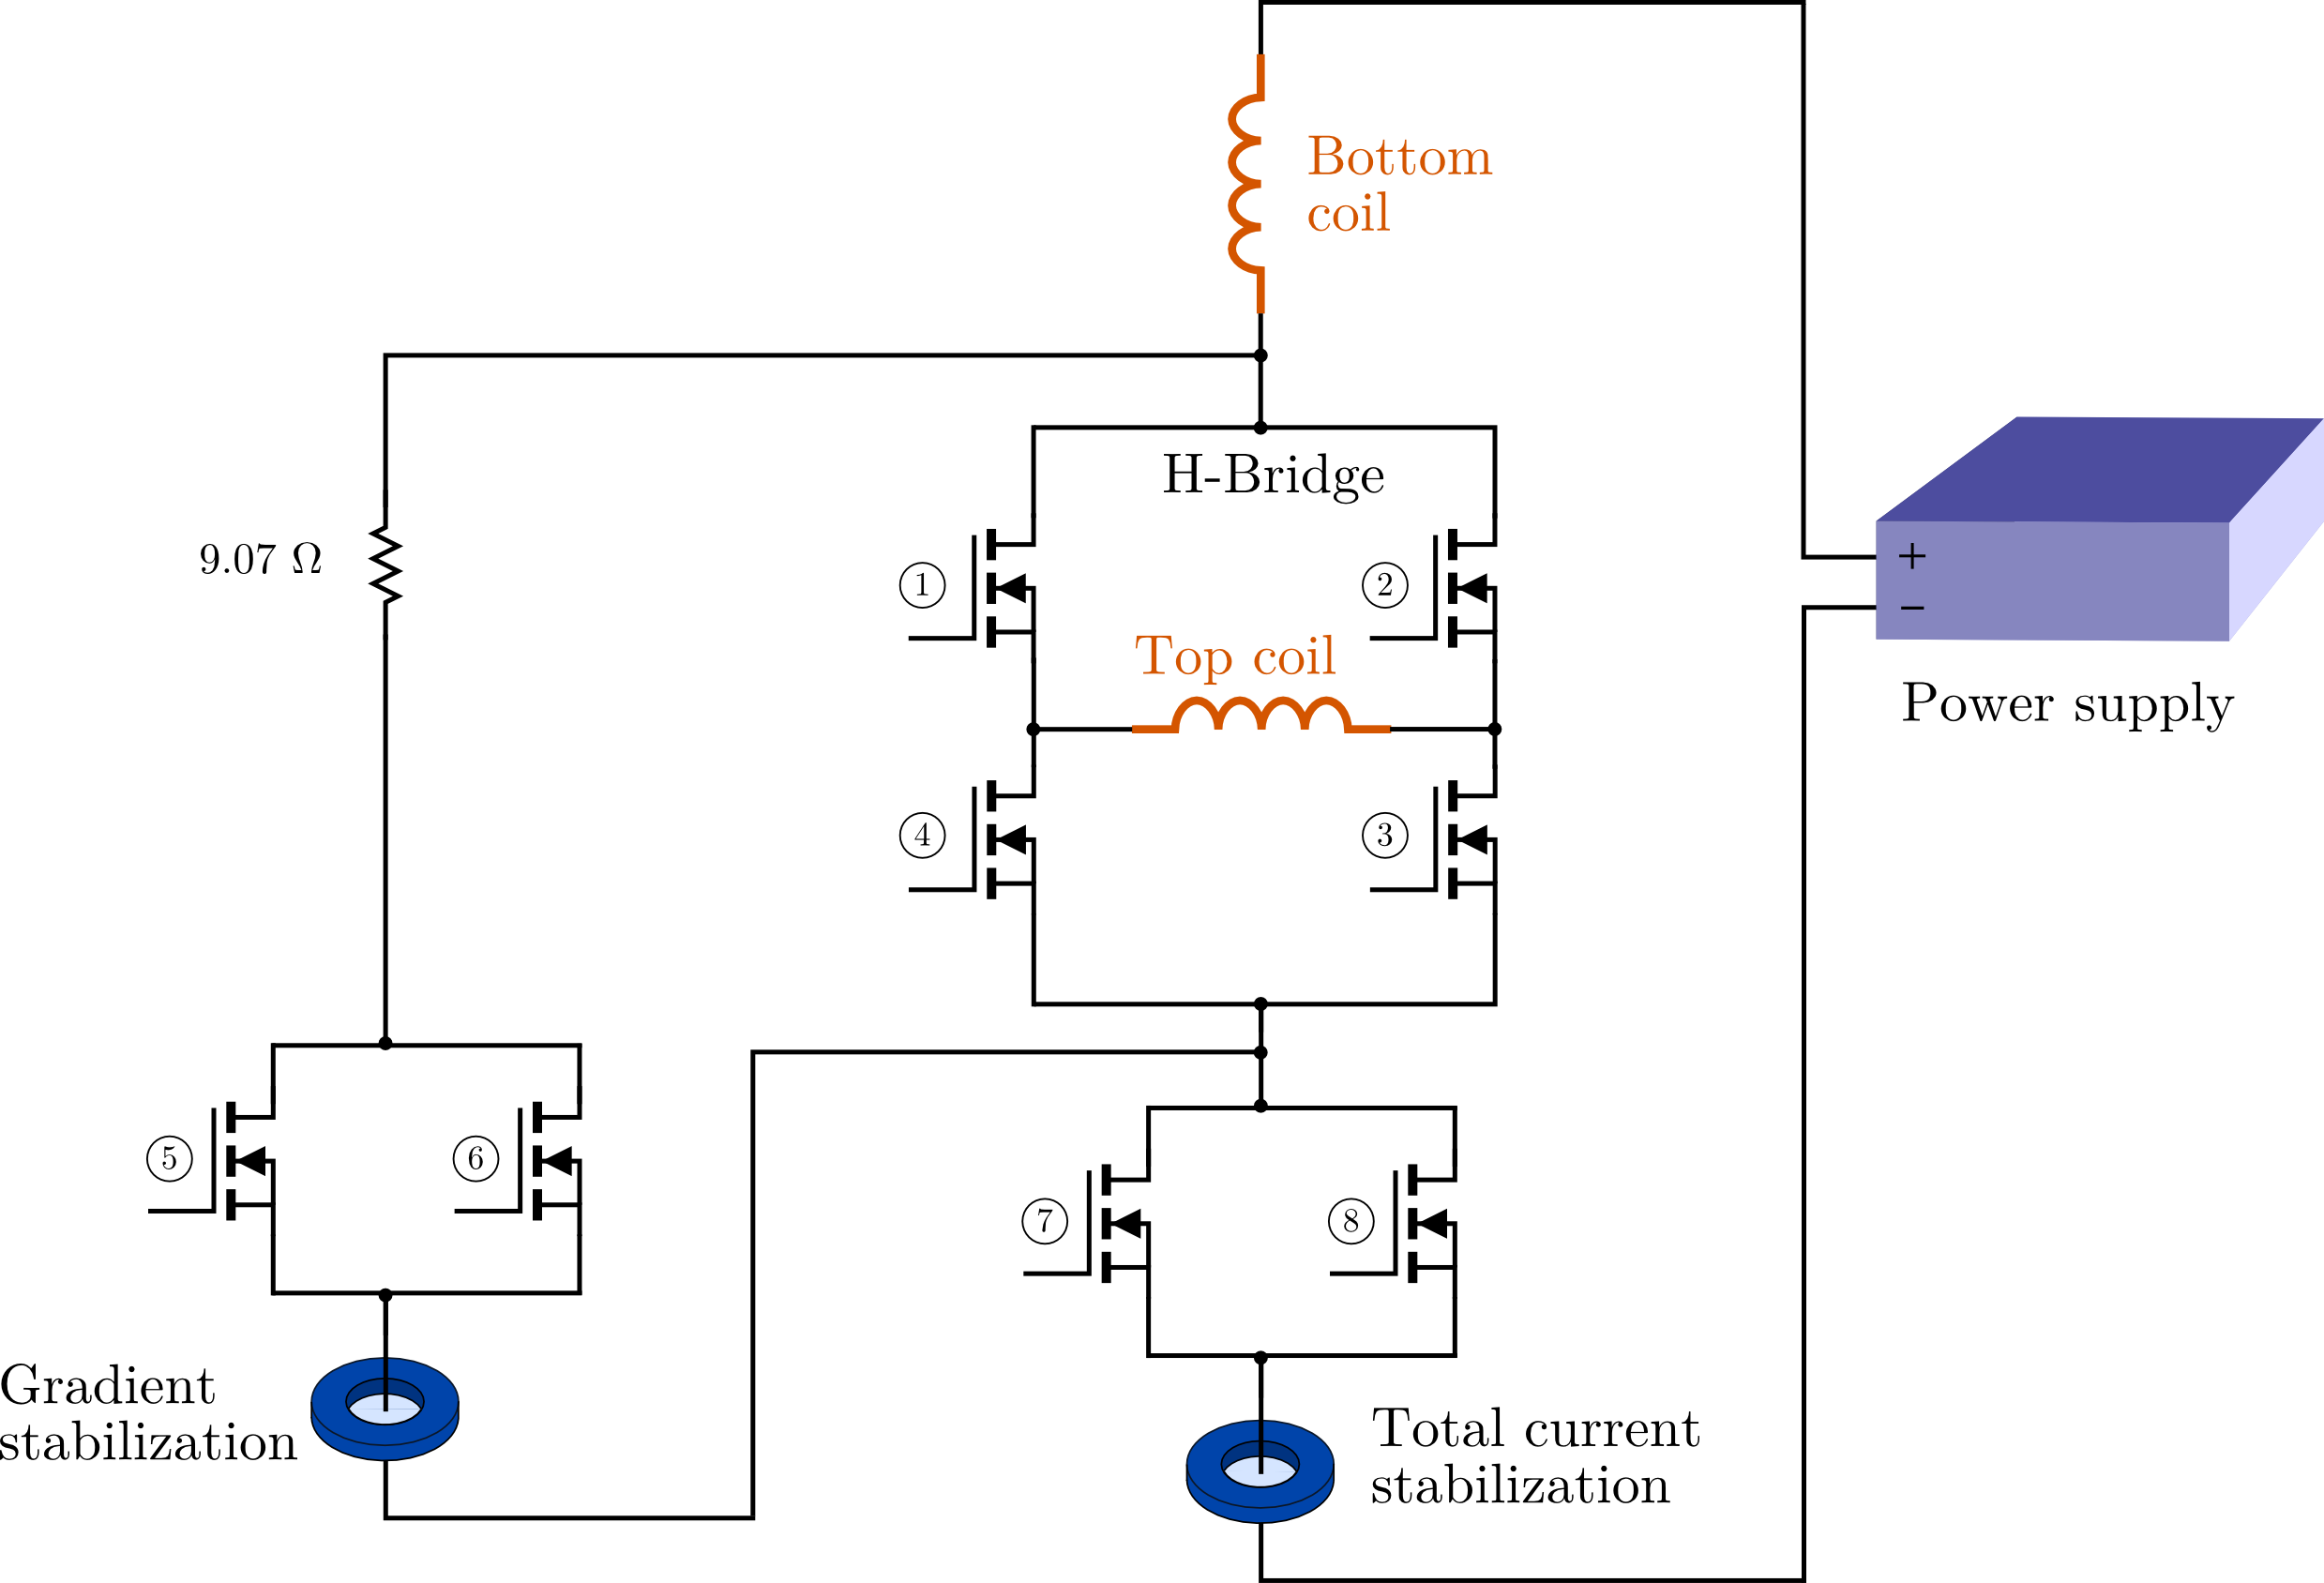
\includegraphics[width=0.85\textwidth]{../masters-figures/coils/fieldcontrol.png}
\caption[Magnetic field control circuit]{\small Schematic of the magnetic field
stabilization circuit.  An H-bridge is used to reverse the polarity of the
current on the top coil.  Current is shunted from the top coil to stabilize the
residual gradient and levitate the atoms.  Current transducers (blue rings) are used
for feedback control of the total current in the system and the current shunted
off the top coil. 
FETs in the H-bridge are Part Num.
STE180NE10.  All other FETs are Part Num. IXFN230N10.  Transient voltage
suppressors, Part Num. 15KW90CA, are used across all the FETs to reduce any
voltage spikes and increase the turn-off speed of the coils.}
\label{fig:fieldcircuit} 
\end{figure} 
The total current through the system is measured  using a Danfisik Ultrastab
866 current transducer, which acts as the source of feedback for stabilization.
For the current shunted for levitation, the transducer used is an LEM HTB-200.
The power supply is a  15~kW Lambda Genesys (80~V, 187.5~A),  operated in
constant voltage mode. A feed forward scheme is implemented to set the voltage
output of the power supply so that the control FETs  do not have to dissipate
too much power.  

%To perform fast magnetic field ramping we override the feed
%forward circuit and set the power supply to a large enough voltage well in
%advance ($\sim$100 ms) for its capacitors to charge up and let the FET's do
%the fast ramping.   In this way we are able to go to from 0 to 120 A in 5 ms.
%although, performing an imaging resonance we find that it takes another 40 ms
%for the field to reach full stability at the top.
%For quick turn off we have
%measured it takes 100 $\mu$s to go from a current of 20 A to zero after
%grounding the gate of the control FETs.  The maximum current we can achieve is
%130 A which can take the field up to 884 G, past the center of the Feshbach
%resonance at 834 G.   



%########################################
\section{Loading the ODT}
\label{sec:odtload}
%########################################

To load the atoms into the ODT one simply needs to turn the ODT light at
maximum power a few ms before the UVMOT is switched on ($t=0$ in the timing
diagram of Fig.~\ref{fig:timingUV}).  We currently turn on the ODT 70~ms before
$t=0$, so it overlaps in time with the 671~nm MOT.  The operation of the 671~nm
MOT is not harmed at all by the presence of the ODT, owing to a small
differential polarizability between the ground $\twos{1/2}$  and excited
$\twop{3/2}$ states~\cite{Safronova2012}.  In other words, both ground and
excited states shift by an equal amount when in the presence of the 1070~nm ODT
light, and thus the laser cooling process is not affected by the presence of
the ODT.   

A wavelength of light where the differential polarizability for a certain
transition vanishes is referred to as a magic wavelength.
Figure~\ref{fig:safronova2p} shows the polarizabilities for the $2S$ and $2P$
states of \li\,  and gives exact values for the magic wavelengths of
$\twop{3/2}$ states.  There is small variability with wavelength around the
wavelength of the ODT (1070~nm),  and the differential polarizability is small.
A calculation (Fig.~\ref{fig:lightshift-calc}) reveals that, for the maximum
intensity of the ODT, a maximum shift of $\sim 1.5\Gamma$ is expected, where
$\Gamma$ is the linewidth of the 671~nm transition. 
\begin{figure}
\centering
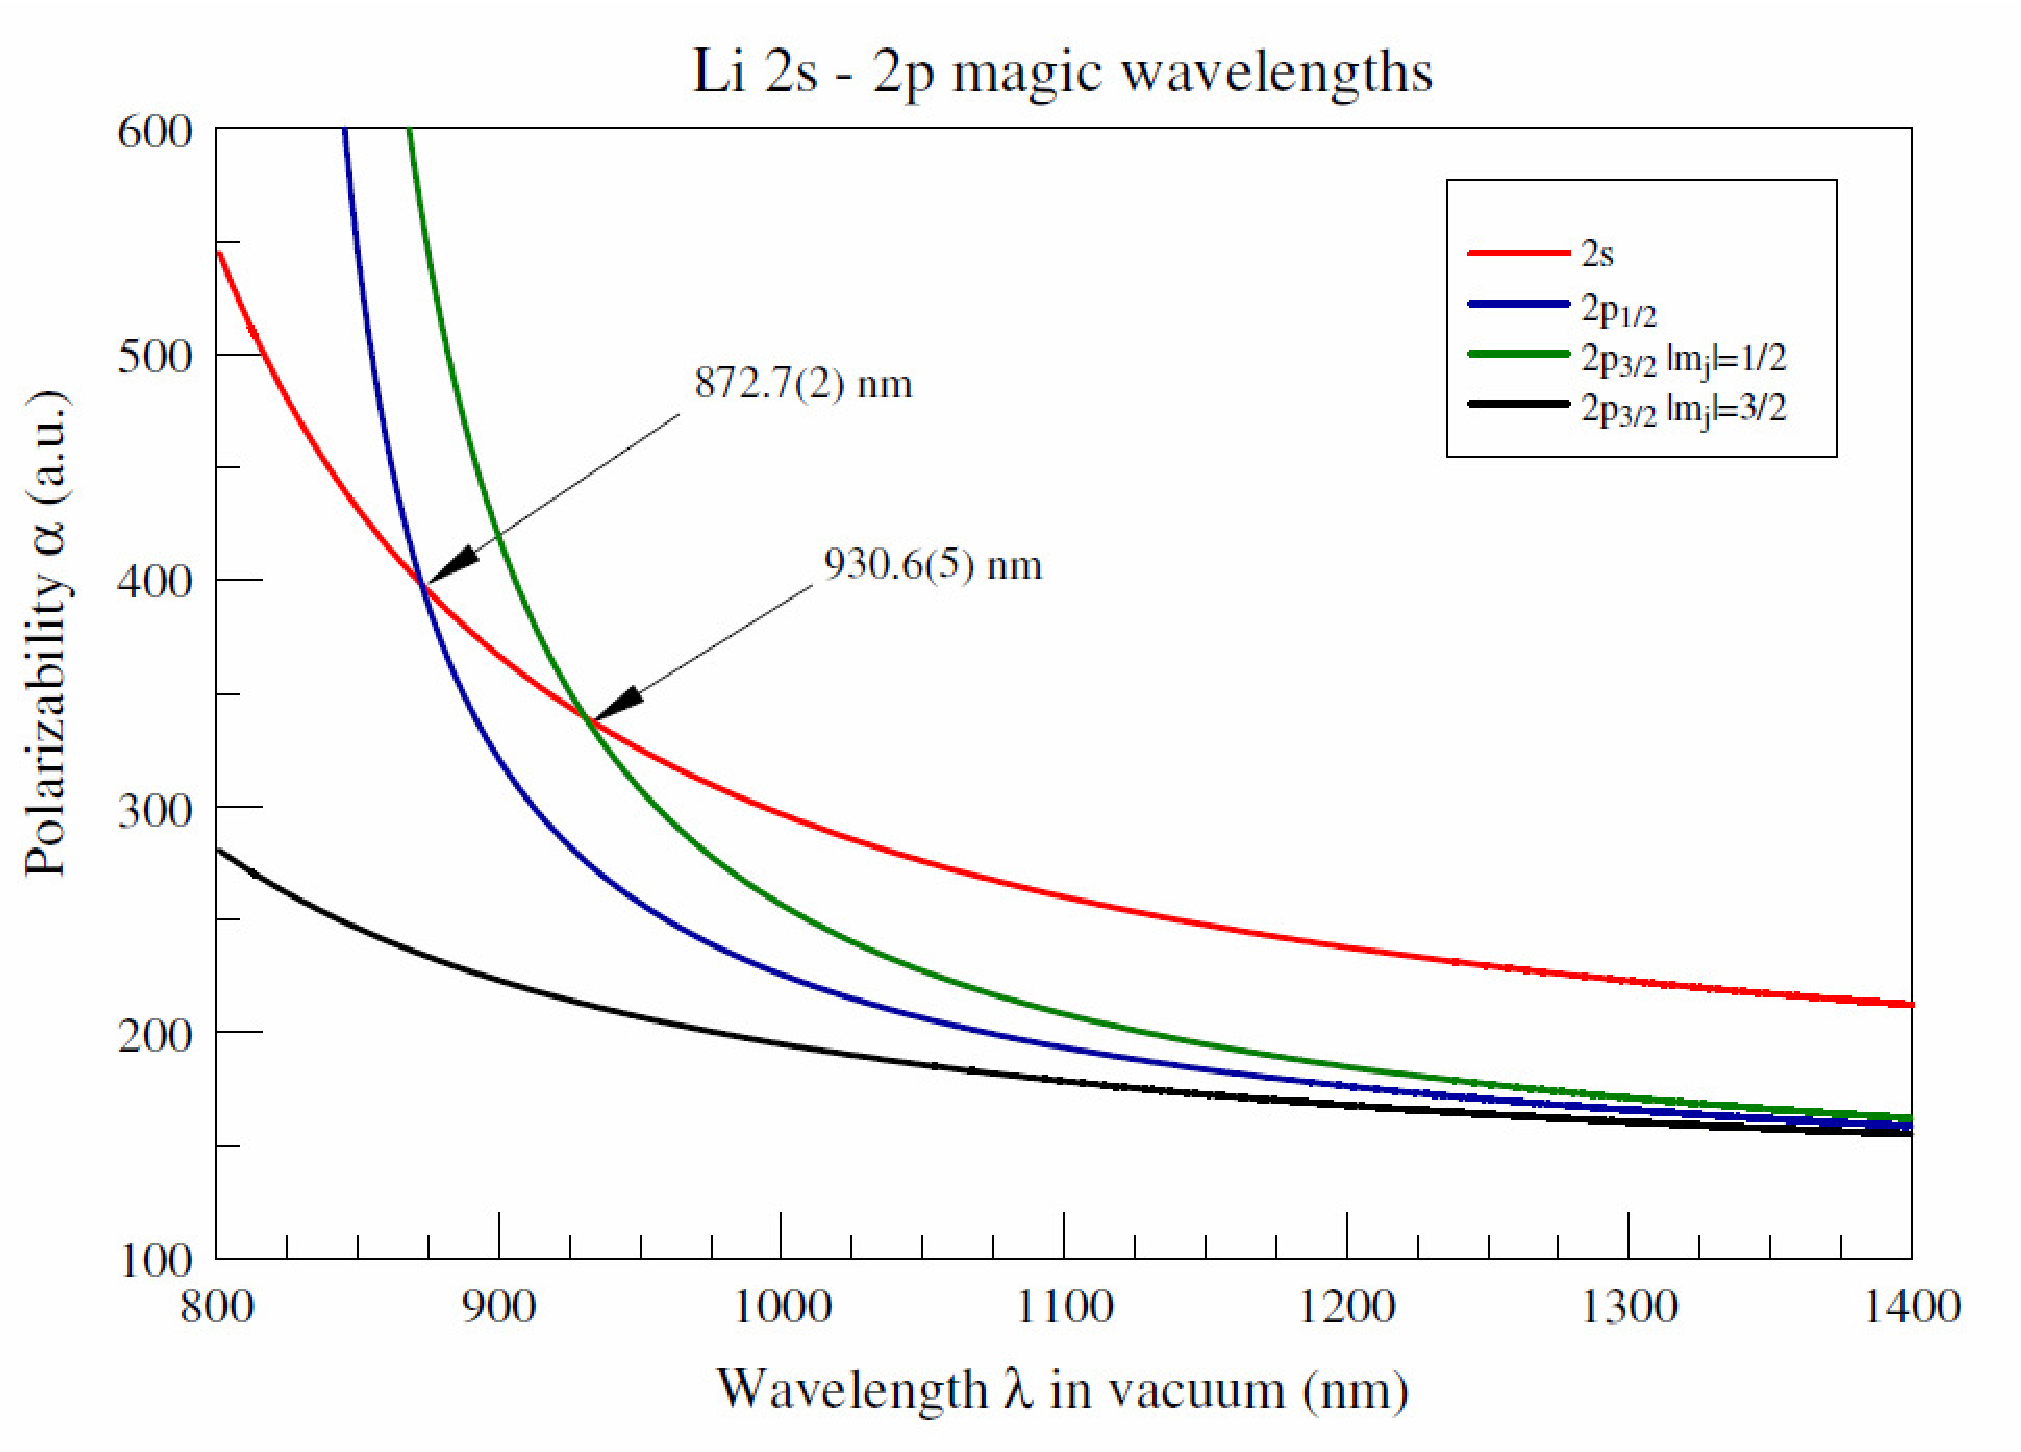
\includegraphics[width=0.65\textwidth]{../masters-figures/safronova/2s2p.pdf}
\caption[Polarizabilities for 1070 nm light]{\small Polarizability in atomic
units for the $2S$ and $2P$ states. Magic wavelengths are indicated by the
arrows.   The atomic units for polarizability (a.u.) can be converted to SI
units (C\,m$^{2}$\,V$^{-1}$) by multiplying by
1.648$\times10^{-41}$~\cite{Safronova2006,Safronova2010}.}
\label{fig:safronova2p} 
\end{figure} 

The situation is different for the \uv\ transition, see
Fig.~\ref{fig:safronova3p}.  In that case, if the wavelength differs much from
a magic wavelength, the differential polarizability of the transition can
become very large.  A calculation for our trap (Fig.~\ref{fig:lightshift-calc})
reveals that for the ODT wavelength of 1070~nm a light shift of at most a few
linewidths is expected at the deepest point in the trap.   It was a great
coincidence that the magic wavelength for the \uv\ transition happened to be so
close to the operating wavelength of our ODT laser.   Being able to continue to
laser cool atoms that are in the volume of the trap greatly enhances the number
of atoms that can be loaded into the ODT,  which can be as large as $\sim
1.4\times 10^{7}$ atoms.  
\begin{figure}
\centering
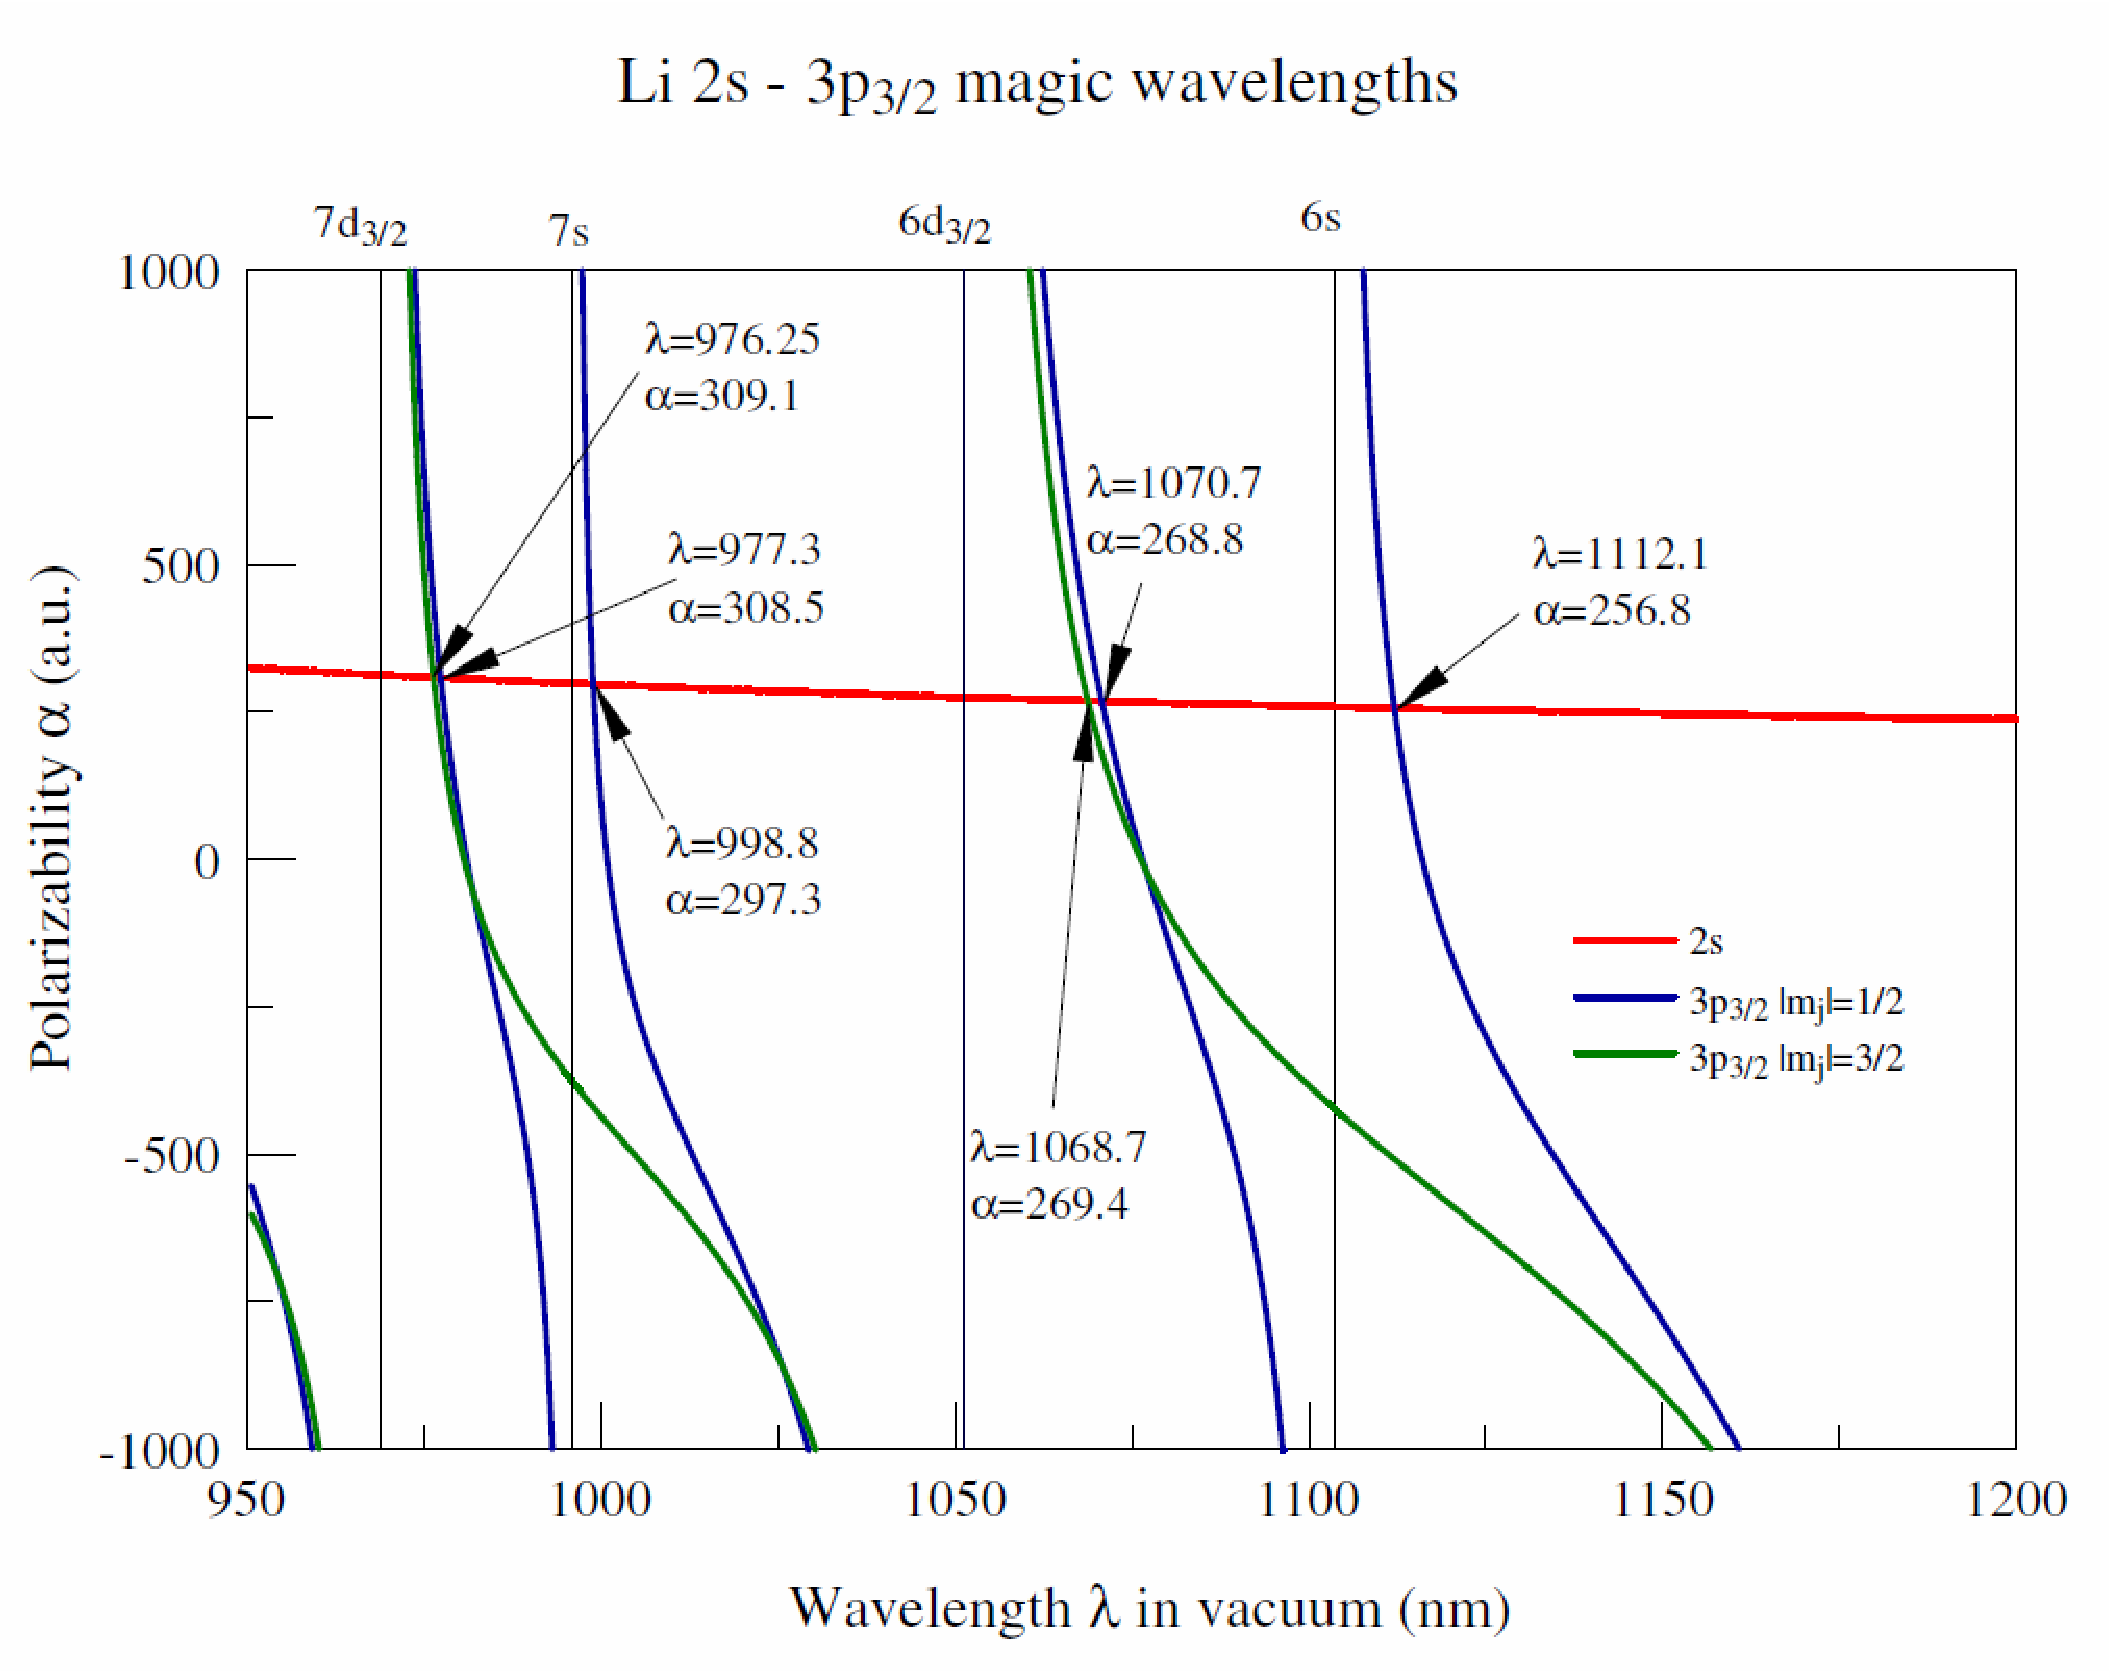
\includegraphics[width=0.65\textwidth]{../masters-figures/safronova/2s3p.pdf}
\caption[Polarizabilities for 1070 nm light]{\small Polarizability in atomic
units of the $2S$ and $3P$ states.  The atomic units for polarizability can be
converted to SI units (C\,m$^{2}$\,V$^{-1}$) by multiplying by
1.648$\times10^{-41}$~\cite{Safronova2006,Safronova2010}.}
\label{fig:safronova3p} 
\end{figure} 

As was briefly mentioned in \S\ref{subsec:mot-uvmot}, we change the detuning of
the 323~nm light in order to optimize the number of atoms loaded into the ODT.
We find that shifting the frequency of the light by $+1$~MHz optimizes
the number loaded.   We also measured the light shift of the \uv\ transition in
our ODT and find that, in the presence of the full power ODT,  the transition
is shifted $\sim 800\,$kHz to the blue,  see Fig.~\ref{fig:lightshift-meas}. 
\begin{figure}
\centering
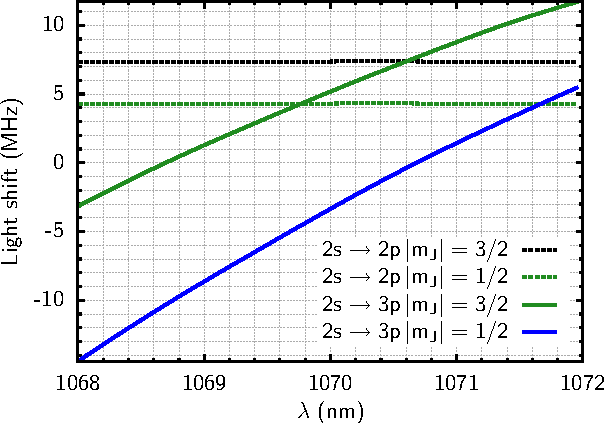
\includegraphics[width=0.6\textwidth]{../masters-figures/safronova/diffpoleps.pdf}
\caption[Differential AC Stark shift for 1070 nm light]{\small Differential AC
Stark shift of the \red and \uv transitions as a function of wavelength for an
intensity of 910 kW/cm$^{2}$ (the maximum intensity the ODT can provide),
calculation by M.~Safronova (personal communication).   }
\label{fig:lightshift-calc} 
\end{figure}
\begin{figure}
\centering
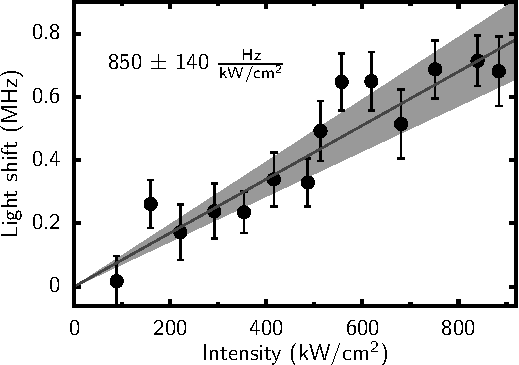
\includegraphics[width=0.6\textwidth]{../masters-figures/lightshift/lightshifteps.pdf}
\caption[Differential AC Stark shift for 1070 nm light]{\small Differential AC
Stark shift of the \uv transition as a function of intensity of the optical
trapping light at $\lambda=1070\,\mathrm{nm}$.  The circles represent the
center of a Gaussian fit of a loss resonance, obtained by heating up atoms in
the ODT with a single UV beam.  The error bars are 1 $\sigma$ statistical error
of the resonance fits.  The solid line is a linear fit to the resonance
position with a slope of $850\pm140 \,\mathrm{Hz/(kW/cm^{2})}$, where the error
(indicated in the plot by the gray shaded area) represents the statistical
uncertainty of the fit and a systematic uncertainty of 10\% on the value of the
trap intensity.  }
\label{fig:lightshift-meas} 
\end{figure}

\subsubsection{Spin mixture} 

Our experiments are realized with a spin mixture of atoms in the two lowest
hyperfine states,  labeled $|1\rangle$ and $|2\rangle$ in
Fig.~\ref{fig:zeemanlevels}.   To create such a spin mixture, we simply turn
off the UV repumping beam 0.5~ms before turning off the UV trapping beam, after
the atoms have been loaded into the ODT.   In that brief time the trapping light
optically pumps all of the atoms into the $F=1/2$ hyperfine state, creating a
balanced mixture of the two hyperfine spin levels. 

After shutting off the UV repumping beam, we turn off the UVMOT magnetic field
gradient, switch the polarity of the top coil,  and ramp up a bias field of
$340~$G, where the scattering length is $\sim -280a_{0}$. The scattering
length is large enough that it leads to efficient evaporative cooling in the
trap.   From this point on, we perform forced evaporation by reducing the power
of the ODT beams.  As the ODT is evaporated away we ramp up a dimple potential,
described in the next section,  such that when the ODT is fully evaporated
away we are left with a degenerate spin mixture in the dimple at a temperature
$T/T_{F}\approx 0.04 $.  The details of the evaporation trajectory will be
discussed later in Chapter~\ref{chap:expprocedures}. 


%########################################
\section{Compensated optical lattice}
%########################################

The compensated optical lattice is the potential in which we realize the
Hubbard model and  carry out all our experiments.   In
Chapter~\ref{chap:compensated-optical-lattice} and Appendix~\ref{app:lattice}
we give much more details about the compensated optical lattice.  In this
section we will give an overview of the setup used to create the potential.

%The optical lattice uses 1064~nm light, red detuned from the 671~nm transition
%such that the light field attracts atoms.   The compensation uses 532~nm light,
%blue detuned from the 671~nm transition, and thus is a potential that repels
%atoms.  

\subsection{Optical lattice and dimple}

An optical lattice potential results due to the stationary interference pattern
of two or more laser beams.   The simplest configuration consists of a laser
beam that is retroreflected upon itself.  We have used this basic
configuration and added a variable liquid crystal retarder LCR, along with a
quarter waveplate and a half waveplate,  in front of the retro-reflection
mirror, as shown in the simplified schematic in Fig.~\ref{fig:simple-latt}.  The
LCR allows us to set the polarization of the retro-reflected beam.  If the
polarization of the retroreflected beam is equal to the polarization of the
incident beam, and both are linear,  then the potential will be a lattice
potential.  On the other hand, if the polarization of the retroreflected beam is
perpendicular to that of the input, there will be no interference and the
potential will be a regular trap.
\begin{figure}
\centering
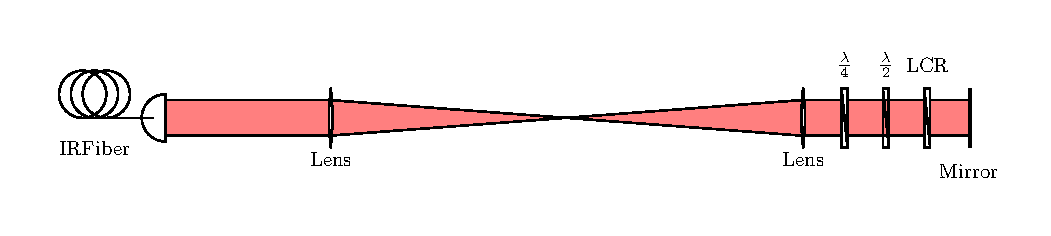
\includegraphics[width=0.8\textwidth]{../ernie-figures/lattice/simple-assembly/latticesassembly.pdf}
\caption[Simplified lattice axis]{\small Simplified setup for a one-dimensional
lattice.   In our implementation we have included waveplates and a variable
liquid crystal retarder (LCR). This allows us to control the polarization of
the retroreflection.  }
\label{fig:simple-latt} 
\end{figure}

We have setups like the one shown in Fig.~\ref{fig:simple-latt} along three
orthogonal axes in order to form a simple cubic lattice potential.   The waist
of each beam is $\sim45\mu$m and thus the intersection region of all three
beams is quite small.  When the polarization of the retro beams is set
perpendicular to the input polarization, we refer to the trap formed at the
intersection of all three axes as the \textbf{dimple trap}.  The dimple trap
provides an excellent starting point for our experiments.   The large
confinement strength resulting from the small volume of the trap leads to efficient
evaporation.  In the dimple we can routinely achieve temperatures as low as
$T/T_{F}\approx 0.04$.  By comparison, in the ODT  one has to spend
considerable effort optimizing the evaporation trajectory, alignment, and beam
profile of the ODT beams to get below $T/T_{F}\approx0.05$, and routinely the
ODT can only get down to $T/T_{F}\approx 0.15$. 


\subsection{Compensation} 

The compensation is a repulsive potential used to tune the amount of
confinement produced by the optical lattice.  An illustration of this idea is
shown in Fig.~\ref{fig:green-push-cartoon}. 
\begin{figure}
\centering
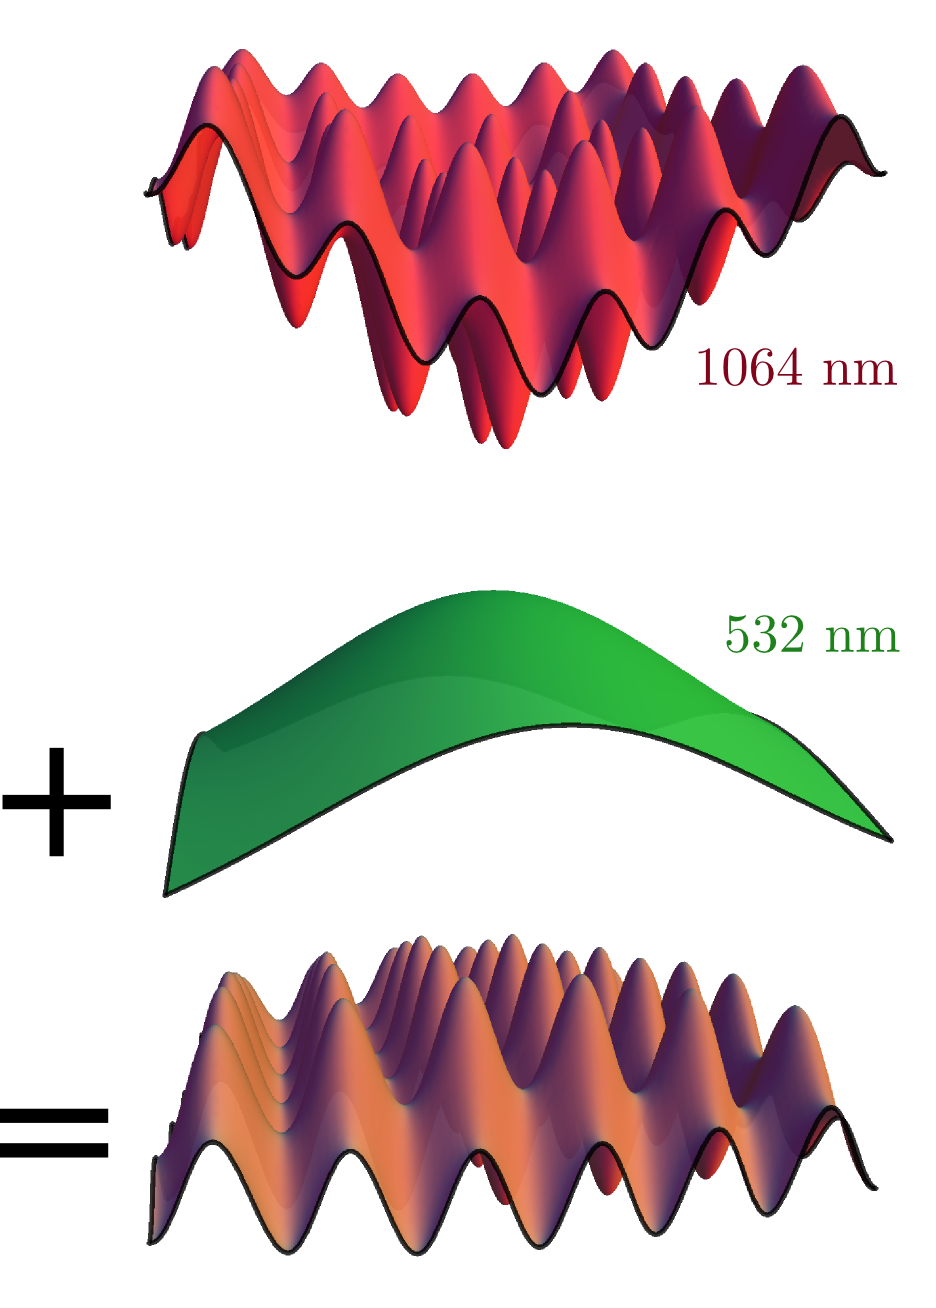
\includegraphics[width=0.35\textwidth]{../figures/setup-overview/compensation-push-cartoon.png}
\caption[Compensation]{\small Illustration of the concept behind a compensated
optical lattice. }  
\label{fig:green-push-cartoon} 
\end{figure}
Adjusting the density of the sample is critical when trying to access the
different phases of the Hubbard model.  Furthermore the compensation was
designed such that it enables the possibility of continuing to evaporatively
cool the atoms once they are in the lattice potential (this will be discussed
in Chapter~\ref{chap:compensated-optical-lattice}.  Reaching lower temperatures
in an optical lattice is a major goal for quantum simulation with ultracold
atoms. 

The compensating potential is formed by Gaussian beams that co-propagate with
the incident lattice beams but are not retroreflected.  A schematic of the
compensation plus optical lattice setup is shown in
Fig.~\ref{fig:comp-latt-schem}.   The details of this setup are described in
detail in Ernie Yang's Master's thesis~\cite{ErnieMs}.  
\begin{figure}
\centering
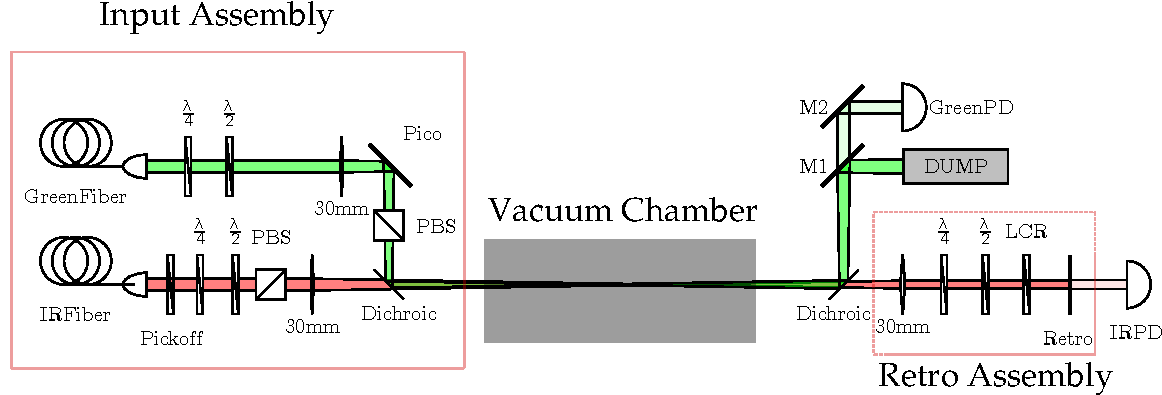
\includegraphics[width=0.8\textwidth]{../ernie-figures/lattice/assembly/latticesassembly.pdf}
\caption[Compensated lattice axis]{\small Compensated optical lattice setup
along one of the three axes.  More details regarding the construction of the
setup can be found in Ernie Yang's Master's thesis~\cite{ErnieMs}}
\label{fig:comp-latt-schem} 
\end{figure}
The light that is coming out of the fibers in Fig.~\ref{fig:comp-latt-schem} is
prepared in a separate optical table.  For the lattice we use 1064~nm light
from a single mode IPG Photonics fiber laser.   The optical layout is shown in
Fig.~\ref{fig:1064setup}.   For the compensation we use 532~nm light from a
Coherent Verdi.  The optical layout is shown in Fig.~\ref{fig:532setup}. 
 
\begin{figure}
\centering
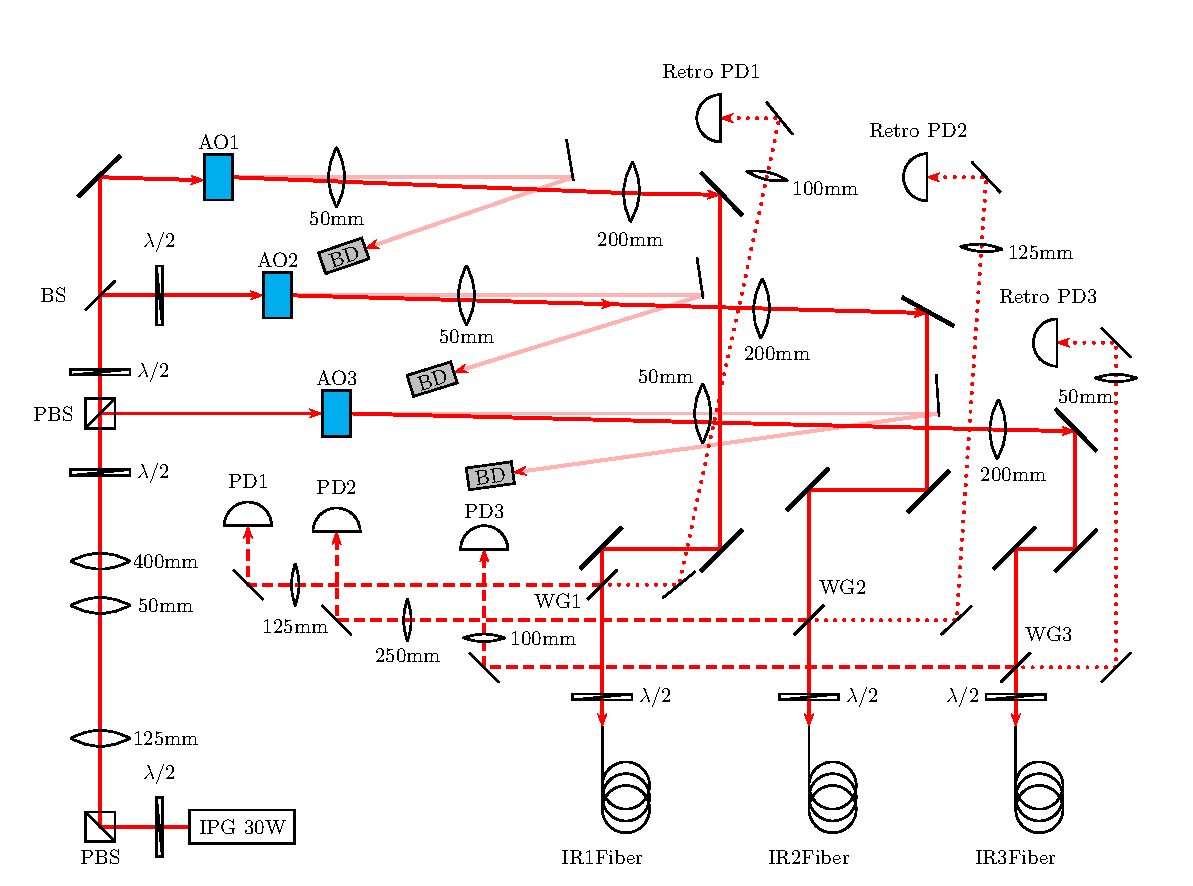
\includegraphics[width=\textwidth]{../ernie-figures/lattice/setup/lattices.pdf}
\caption[1064~nm setup]{\small Optical setup showing how the 1064~nm light from
the 30~W IPG laser is split up before coupling into the fibers for each of the
three lattice axes. The acousto-optic modulators, labeled AO1-3, are used for
intensity stabilization of the intensity.   Feedback to these AOs comes from
the photodetector labeled IRPD in Fig.~\ref{fig:comp-latt-schem}.  The driving
frequencies of AOs 1-3 is 70, 80, and 90 MHz respectively, with the offset used
to avoid interference between the different lattice axes.  }
\label{fig:1064setup} 
\end{figure}
\begin{figure}
\centering
\includegraphics[width=\textwidth]{../ernie-figures/lattice/setup/green.pdf}
\caption[532~nm setup]{\small Optical setup showing how the 532~nm light from
the Coherent Verdi is split up before coupling into the fibers for each of the
three lattice axes. The acousto-optic modulators, labeled AO1-3, are used for
intensity stabilization of the intensity.   Feedback to these AO's comes from
the photodetector labeled GreenPD in Fig.~\ref{fig:comp-latt-schem}. The
driving frequencies of AOs 1-3 is 80, 88, and 72 MHz respectively, with the
offset used to avoid interference between the different compensation axes. }
\label{fig:532setup} 
\end{figure}




%########################################
\section{Diagnostics}
%########################################

Having described all the systems that we use to manipulate the atoms, we will
now describe very generally the systems used to measure their properties.  For
diagnostics we exploit again the strong interaction of the atoms with near
resonant light.   We can perform fluorescence, absorption and phase contrast
imaging of the atoms.   We have also built a setup to measure  Bragg scattering
of light, a probe of the crystalline and spin order of atoms in a
lattice~\cite{Ted2010}. A detailed description of the Bragg scattering setup will be
presented in Chapter~\ref{chap:bragg-scatt}.    

For the purposes of imaging the MOT and UVMOT, which can reach a spatial extent
of up to several mm after TOF expansion, we use fluorescence imaging
using a surveillance CCD camera, see Fig.~\ref{fig:diagnostics}. 

To image the smaller samples (tens of $\mu$m) in the ODT, the dimple, or the
optical lattice,  we use a nearly diffraction limited relay lens system
(Fig.~\ref{fig:relaylens}) which creates a real image of the atoms outside the
vacuum chamber.  The numerical aperture (NA=0.16) of the relay lens determines
the resolution of the imaging system
($\sigma_{\mathrm{res}}\approx3\,\mu$m)\footnote{Here the resolution of the
imaging system is defined as the $1/e$ radius of the point-spread function PSF
of the imaging system, $\mathrm{PSF}(x)\propto \exp\left[
-\frac{x^{2}}{\sigma_{\mathrm{res}}^{2}} \right]$.  The size of the PSF was
obtained by fitting images of a 1951 USAF test target.}.   A commercial
microscope objective is then used, in conjunction with a Nikon telephoto lens,
to image the the relayed image of the atoms onto a CCD.   The setup is shown in
Fig.~\ref{fig:diagnostics}, 

\begin{figure}
\includegraphics[width=\textwidth]{../masters-figures/imaging/setup.pdf}
\caption[Diagnostics setup]{\small This figure shows instruments that we use
for diagnostics.  A photodiode can be used for basic monitoring of the MOT
loading level.  Fluorescence imaging with the Basler CCD camera is used to
characterize the MOT and UVMOT.   Smaller samples in the ODT and optical
lattice are imaged using a relay lens (not shown). A microscope objective and
Nikon telephoto lens, project the image of the atoms onto the Andor iXon EMCCD
camera (DU-897-E).}  
\label{fig:diagnostics} 
\end{figure}
 
\begin{figure} \centering
\includegraphics[width=0.85\textwidth]{../masters-figures/imaging/relay.pdf}
\caption[Relay lens system]{\small  Relay lens system to form an image of the
atoms outside the vacuum chamber. A re-entrant imaging viewport on the vacuum
chamber allows placing a 1 inch diameter lens 80~mm away from the atom sample.
Both lenses are Part Num. GPX-30-80 gradient index plano-convex lenses from
LightPath Technologies.  }
\label{fig:relaylens} \end{figure} 



%########################################
\section{Control, automation, and data analysis}
%########################################

Finally, we describe the computer control system that orchestrates the
behavior of all other systems in our experiment.   The control system is is
based on the National Instruments PXI chassis NI-PXIe1062Q.   

The chassis hosts
three 6733 Analog Output cards and a 6259 Multifunction DAQ card.   An experimental
sequence consists of a series of TTL pulses that control the timing of events
related to instruments on the apparatus.  The clock to which TTL pulses are
synchronized is an 80~MHz oscillator on the 6259 Multifunction DAQ card.    A
digital sequence can have a maximum output rate of 10 MHz (resolution time step
of 1 $\mu$s) and at this output rate the buffer can hold sequences that last
several tens of seconds.  We use the analog output channels of the PXI system
as one typically uses arbitrary waveform generators; waveform outputs can be
triggered by TTL pulses at any given time during the experimental sequence.
The timebase for arbitrary waveform outputs on analog output channels is the
on-board oscillator of each card.  For the 6259 it is a 80~MHz oscillator and
for the 6733 it is a 20~MHz oscillator.  

The experimental sequences, including all waveform outputs,  are programmed in
a format based on the Python programming language.  This makes it very easy to
program new sequences and recycle parts of old sequences.    The Python  based
sequence code is interpreted by a program also written in Python which produces
a raw sequence output file that contains all the TTL timings and the waveforms
for a particular experiment.  The raw sequence output is read by LabVIEW, which
takes care of outputting the sequence on the TTL and analog output channels.  

In an experimental cycle, the MOT is loaded until a certain fluorescence is
reached. At that point a trigger synchronized with the 60~Hz mains starts the
output of the experimental sequence. 



%%%%%%%%%%%%%%%%%%%%%%%%%%%%%%%%%%%%%%%%%%%%%%%%%%%%%%%%%%%%%%%%%%%%%%%%%%%%%%%
%%%%%%%%%%%%%%%%%%%%%%%%%%%%%%%%%%%%%%%%%%%%%%%%%%%%%%%%%%%%%%%%%%%%%%%%%%%%%%%
%%%%  CHAPTER 5 
%%%%%%%%%%%%%%%%%%%%%%%%%%%%%%%%%%%%%%%%%%%%%%%%%%%%%%%%%%%%%%%%%%%%%%%%%%%%%%%
%%%%%%%%%%%%%%%%%%%%%%%%%%%%%%%%%%%%%%%%%%%%%%%%%%%%%%%%%%%%%%%%%%%%%%%%%%%%%%%
\chapter{Compensated optical lattice potential}
\label{chap:compensated-optical-lattice}


One of the most important aspects of the work presented in this thesis has been
the design and construction of the potential in which our experiments take
place.   In previous chapters we have referred to ultracold atoms in optical
lattices as a nearly ideal realization of the Hubbard model.   In fact, there
are important differences between ultracold atoms in optical lattices and
idealized models.    

To start with, optical lattices are created with finite laser beams, and thus
the value of the lattice depth is never constant throughout the sample.      In
addition, when using ultracold atoms one is forced to use an overall confining
potential, to achieve large enough densities close to one particle per site
(half-filling) such that the effects of correlations between particles become
manifest.  An illustration of these ideas is shown in
Fig.~\ref{fig:comp-uncomp}. 
\begin{figure}
    \centering
\includegraphics[width=\textwidth]{../illustrations/lattice/comp+uncomp-inhom.png}
\caption{\small In an ideal system (left) a lattice is homogeneous and flat,
extending to infinity.  For a finite number of particles the density would go
to zero, as the gas continues to expand in the lattice.   For real Gaussian
beams (center), the lattice is inhomogeneous.  Notice that the inhomogeneity of
the lattice beams results in a small amount of confinement (curvature of lower
envelope of the potential), but not sufficient to increase the density
significantly.   Additional confinement (right) must be provided to achieve the
necessary densities with a finite number of particles.  } 
\label{fig:comp-uncomp}
\end{figure}
In recent years there has been significant work in trying to make
``square-well'' potentials, that are flat but have very steep
walls~\cite{liang20091,PhysRevLett.110.200406}.  In such potentials one could
reach densities near half-filling and have a homogeneous lattice depth at the
same time.  This approach, to our knowledge, has not yet been realized with
optical lattices.

Experiments in lattices have traditionally dealt with at least one of the
problems stated above: the inhomogeneity of the lattice depth.    Typically,
experiments use lattice beam waists that are large comparable to the size of
the system.   An additional Gaussian beam (or arrangement of beams) with
smaller waists provides the external confinement and determines the size of the
system.   This approach has the advantage that the lattice depth, being nearly
constant throughout the extent of the sample, results in Hubbard parameters $t$
and $U$ that are also nearly constant throughout the sample. In any case, the
density distribution of the atoms still remains inhomogeneous due to the
external confinement, and that presents a problem for the interpretation of
bulk measurements.   Furthermore, the traditional setup (large beam waist +
additional confinement)  has a disadvantage that has to do with the possibility
of continuing to evaporatively cool the atoms once they are loaded into the
lattice potential.  

The field of ultracold atomic physics has built its success by exploiting the
power of two very effective atom cooling techniques, laser cooling and
evaporative cooling.  The former makes use of dissipative forces imparted by
light on atoms to decelerate their center of mass motion,  and has helped
bridge the gap from the Kelvin to the microKelvin regime.  The latter takes
over at the limit of laser cooling and is able to take the samples deep into
quantum degeneracy.  Evaporative cooling works on a simple principle: when a
particle, with energy larger than the mean energy per particle of the system,
escapes the potential, then mean energy per particle of the system decreases.
After an elastic collision between a pair of atoms, there is a probability that
one of them may have enough energy to escape the trap.  But this probability
becomes negligible if the trap is too deep, which renders evaporative cooling
ineffective. 


In our work we have chosen to trade-off the uniformity of the Hubbard
parameters, $t$ and $U$, in exchange for the possibility of continuing to
evaporatively cool the atoms once they are loaded into the optical lattice.
The goal of this experiment has been to create an antiferromagnetic (AFM) Mott
insulator in the center of the trap, and continued evaporative cooling in the
lattice is a promising path to that end.  As we will see, our lattice setup
uses lattice beam waists that are comparable to the size of the sample.   The
inhomogeneity of the lattice is thus very pronounced, and the lattice beams
alone confine the atoms in excess, as shown in Fig.~\ref{fig:comp-uncomp2}. 
\begin{figure}
    \centering
\includegraphics[width=0.78\textwidth]{../illustrations/lattice/comp+uncomp-inhom2.png}
\caption{\small A lattice with beam waist comparable to the extent of the sample
(left)  produces excessive confinement, resulting in densities above
half-filling at the center.  Compensation is added (right) to reduce the
confinement and tune the density.  In this approach, the sample in the lattice
has the possibility to undergo continued evaporative cooling. }
\label{fig:comp-uncomp2}
\end{figure}
The addition of a repulsive compensation potential allows tuning the peak
density of the system to reasonable values in the vicinity of half-filling, and
pushes up the chemical potential such that atoms have the possibility of
escaping the trap and evaporative cooling becomes effective. 

In this chapter we will use the local density approximation (LDA) in
conjunction with the second order high-temperature series expansion (HTSE) to
calculate the properties of various trapping potentials.   We will compare our
compensated lattice potential with a traditional optical lattice setup with
large beam waists, and we will discuss ways in which further improvements to
our setup can be realized.  In doing this comparison we will keep in mind
practical considerations such as the total atom number required to achieve a
density near half-filling at the center of the trap.  For more technical
aspects of our potential, such as calculation and calibration of beam waists,
and calculation of heating rates, refer to Appendix~\ref{app:lattice}.  


\section{Form of the potential}  

The compensated simple cubic optical lattice potential is formed at the
intersection of three orthogonal axes, see
Fig.~\ref{fig:compensated_lattice_simple_schematic}.  Along each axis, a 1D
lattice potential is formed by retro-reflecting a red-detuned Gaussian beam.
Overlapped onto each of the lattice beams there is a compensation beam, which
is blue-detuned and thus produces a repulsive potential.   The compensation
beam is not retro-reflected, so it does not form a standing wave potential.  
\begin{figure}
    \centering
\includegraphics[width=0.8\textwidth]{../figures/lda_evap/compensated_lattice_simple_schematic.png}
\caption{\small Simplified schematic of the compensated lattice setup along one of the
axes.}\label{fig:compensated_lattice_simple_schematic}
\end{figure}

The lattice beam that propagates along the $x$ axis produces a potential of the
form 
\begin{equation}
  V_{L}( x; y,z)  = 
  - s_{0} \exp\left[- 2 \frac{ y^{2} + z^{2} }{w_{L}^{2}} \right]
  \cos^{2}( k_{L} x ) 
\end{equation}
where $s_{0}$ is the lattice depth at the center of the potential,  $w_{L}$ is
the lattice beam waist and $k_{L} = 2\pi/\lambda_{L}$ is the wavenumber of the
lattice light.
The compensation beam that propagates along $x$ produces a potential  
\begin{equation}
  V_{C}( x; y, z)  = 
   g_{0}  \exp\left[ -2 \frac{ y^{2} + z^{2} }{w_{C}^{2}} \right] 
\label{eq:Vcomp}
\end{equation}
where  $g_{0}$ is the depth (or rather height since it is repulsive) of the
compensating potential, and $w_{C}$ is the beam waist of the compensation beam.

The combined potential of lattice plus compensation for the beams propagating
along $x$ is 
\begin{equation}
  V_{1D}( x; y ,z ) = V_{L}(x; y,z) + V_{C}(x; y, z)
\end{equation}

The total potential for our simple cubic lattice is given by 
\begin{equation}
  V_{3D}(x, y, z)  =  V_{1D}( x; y,z) + V_{1D}( y; z,x) + V_{1D}(z; x,y)
\end{equation}


\section{General aspects}
\label{sec:general_aspects}

%In what follows we will first look at general aspects of the potential, using
%analytic approximations to its shape and considering a zero temperature sample.
%Then we will use the high-temperature series expansion (HTSE)\footnote{ The
%HTSE is  an analytical solution to the Hubbard model that is valid at
%high-temperatures.  The HTSE is very good for $T \gg t$ and works down to $T/t
%\sim 1.8$.  This solution gives us the thermodynamic quantities (density,
%double occupancy, entropy per particle, etc.)  for a homogeneous system.}  and
%the local density approximation (LDA) to study the system in more detail. 

Before we go ahead and deploy the full machinery of the LDA+HTSE we will
discuss some general aspects of the potential using analytical approximations
to its shape and considering a zero temperature sample.  We will find that at a
certain ratio of the lattice to compensation beam waist,    $\awaist \equiv
w_{L}/w_{C}$,  one can create a potential optimal for evaporative cooling,
which is also flat at the bottom, in a way reminiscent of the idealized
square-well potential. We will also make an estimate of the atom number
required to realize this setup.

One of the important things to note, is that at each point in space  we will, in
general, have three different lattice depths, associated with each of the
$x,y,$ and $z$ lattice directions. We denote the lattice depths as $s_{x}$,
$s_{y}$ and $s_{z}$, all of which depend on position. To make things simpler,
we can consider the potential along the 111 direction; along this direction
we have equal lattice depths in $x,y,$ and $z$:
\begin{equation} 
  s_{x}( \rdiag ) = s_{y}( \rdiag ) = s_{z}( \rdiag ) = 
  s_{0} \exp \left[ - \frac{ 4 \rdiag^{2} }{3 w_{L}^{2} } \right]  
  \equiv s(\rdiag) 
\end{equation}
where $\rdiag$ represents the distance along the 111 direction.

The bottom envelope of the lattice potential along 111 is given by 
\begin{equation}
  V_{L,\text{env}}( \rdiag )  = -3 s_{0} 
  \exp \left[ - \frac{ 4 \rdiag^{2} }{3 w_{L}^{2} } \right]  
\end{equation}
At each point in space there is a local band structure determined by
$V_{L,\text{env}}$, $s_{x}$, $s_{y}$, and $s_{z}$.  The lowest energy of the
band, which we will refer to  as $E_{0}$, can be approximated by the zero-point
energy of the 3D harmonic oscillator obtained by Taylor expanding the potential
at a lattice site.   This approximation is only valid for deep
lattices\footnote{Recall that the recoil energy, $E_{r}$, is defined as
$\frac{h^{2}}{8m\lambda^{2}}$, where $m$ is the mass of an atom and $\lambda$
is the wavelength of the lattice. } (refer back to 
Fig.~\ref{fig:bands1d} for reference) but we will use it here for its simplicity: 
\begin{equation} E_{0} =  V_{L,\text{env}} +  
     \frac{3}{2} \hbar \omega_{0}  = V_{L,\text{env}} +  3E_{r}\sqrt{ s/E_{r} }. 
\end{equation} 
We can also obtain an expression for the bandwidth, $W$, of the lowest energy
band valid in the limit of deep lattices (cf. Eq.~\ref{eq:tunnelMathieu} or
Ref.~\cite{Bloch2008}):
\begin{equation}
  W =   12 t 
  = E_{r}\frac{48}{\sqrt{\pi}} (s/E_{r})^{3/4} e^{-2\sqrt{s/E_{r}}} .
\end{equation}
Notice that the quantities $E_{0}$, $W$, $\omega_{0}$, $s$, and $t$ are all
position dependent, and thus functions of $\rdiag$. The profiles of these
quantities (and also of the energy of the first excited band, $E_{1}$) are
shown in Fig.~\ref{fig:lattice_general} for a simple cubic lattice  with
lattice beam waist $w_{L}=47\,\mu$m.  

Notice that the Gaussian profile of the lattice beams, being comparable to the
size of typical samples $\approx 40\,\mu$m,  will provide a significant overall
confinement for the atoms. This is in contrast with traditional setups, where
the lattice beam waist is typically larger than 150~$\mu$m and in the length
scale of typical samples the inhomogeneity of the lattice potential is not
noticeable. 
\begin{figure}
    \centering
\includegraphics[width=0.9\textwidth]{../figures/lda_evap/lattice_general.png}
\caption{\small Profiles along $\rdiag$ for a 7$E_{r}$ lattice with
$w_{L}=47\,\mu$m and $\lambda=1064$\,nm.  The energy levels in the lowest band
of the lattice correspond to the shaded blue region.  The curvature of $E_{0}$
determines the confinement.  }
\label{fig:lattice_general}
\end{figure}


\subsubsection{Compensation}
\label{subsec:compensation}

If the lattice beam waist is comparable to the size of the system (as is the
case in our setup),  the confinement from the lattice itself will bee too
large, and it will result in a very large density\footnote{Since we consider
the single band Hubbard model, the density will be saturated at 2 particles per
lattice site.}.  Repulsive compensation beams are then used  to set the
exact amount of confinement in the system and tune its density. 

Beyond simply tuning the density, one can choose a ratio of lattice to
compensation beam waist, defined as $\awaist = w_{L}/w_{C}$~\cite{Mathy2012},
in order to affect the exact spatial dependence of the lowest band.   A setup
which flattens the profile of the lowest band at the center of the trap can
enlarge the size of a local phase which may exist there, an idea suggested in
Ref.~\cite{Mathy2012}, which is at the heart of our compensated lattice design.
In our implementation with Gaussian beams, the lowest band can be made quartic
at best.  This situation may be ideal, because the flat central part of the
lowest band enlarges the extent of the local phase in the center, and the walls
of the potential are not to steep, which lessens the requirements on the
precision of the atom number required to realize a given phase~\cite{Ma2008}.
Besides flattening the band, the use of compensation enables the possibility of
evaporative cooling the sample in the lattice, as we will explain later on.  


\subsubsection{Power series expansion of the lowest band} With the addition of
repulsive compensation beams (depth $g_{0}$ and beam waist $w_{C}$, as in
Eq.~\ref{eq:Vcomp})  we can expand the lowest band profile of the lattice in a
power series as  
\begin{multline} 
  E_{0}(\rdiag)    \approx   
  3( g_{0} + E_{r}\sqrt{s_{0}/E_{r}} - s_{0} )   
  + \left[ 
    \frac{ 4s_{0} - 2E_{r}\sqrt{s_{0}/E_{r}} }{w_{L}^{2} } 
   - 
  \frac{ 4 g_{0} }{ w_{C}^{2}} \right]
  \rdiag^{2}  \\ 
  +  \left[  \frac{ - 8 s_{0} + 2E_{r}\sqrt{s_{0}/E_{r}} }{3 w_{L}^{4} } + 
    \frac{ 8 g_{0} }{3 w_{C}^{4} }  \right] \rdiag^{4}   + 
  \mathcal{O}( \rdiag^{6} )
\label{eq:series_expansion} 
\end{multline}  

If our interest is to maximally flatten the profile of the lowest band, the
quadratic term in the series expansion can be nulled out if one chooses
\begin{equation}
 g_{0} = \frac{  4 s_{0} - 2 E_{r}\sqrt{s_{0}/E_{r}} }{ 4 \awaist^{2} }  
  \equiv g_{\text{quartic}} . 
\end{equation}
If an AFM phase forms at the center of the trap, this
choice of $g_{0}$ will be the most favorable to enlarge the size of the AFM
domain. 

If $\awaist > 1$ and we use a compensation larger than $g_{\text{quartic}}$,
the band profile will have a bump in the center.  Experimentally we have
observed that in that case it becomes hard to align the compensation beams such
that the sample actually stays at the center of the trap.

In our current experiments we use $s_{0}=7\,E_{r}$, and the beam waists in
our setup are calibrated (see Appendix~\ref{app:lattice} for details about the
calibration procedure) to be approximately $w_{L}=47\,\mu$m and
$w_{C}=40\,\mu$m, which gives $\awaist=1.17$.  The necessary compensation to
flatten the band, according to this simplified analytical model, is then
$g_{\text{quartic}} =  4.1\,E_{r}$.


\subsubsection{Evaporation} 

We want to consider the possibility of evaporative cooling in a sample that has
$n=1$ at the center (as is the case for an AFM Mott insulator).   The density
of the sample determines its Fermi energy and, if the Fermi energy is close to
the energy required to escape the potential, evaporation will be effective.
Here, we will consider a cloud with $n=1$ and will set its Fermi energy to
match the energy threshold for evaporation.   This will determine the
compensation $g_{0}$ required for optimal evaporation.   We then equate this
$g_{0}$ with $g_{\mathrm{quartic}}$, obtained above, to find out the parameters
for a trap that is optimal for evaporation and has a flattened bottom. 

To impose $n=1$ at the center we set the global chemical potential\footnote{At
zero temperature the global chemical potential is equal to the Fermi energy.}
to 
\begin{equation}
  \mu_{\text{global}} \equiv \mu(r_{111}=0) = E_{0}(r_{111}=0) + U/2, 
\end{equation}
 where $U$ is the on-site interaction strength \footnote{ For a discussion of
the thermodynamic properties of the Hubbard model refer to
Chapter~\ref{chap:hubbardmodel}} 
%\footnote{ $n(\mu=\bar{E} + U/2)=1$,  is a property of the Hubbard model valid
%at any temperature,  see Fig.~\ref{fig:HTSEhomogeneousA}.  Notice that we are
%measuring the chemical potential with respect to the zero of the optical
%dipole potential.   In the homogeneous Hubbard model $\mu$ is measured with
%respect to $\bar{E}$, and a more familiar expression is $n(\mu=U/2)=1$ (see
%the discussion after Eq.~\ref{eq:hubbard_not_shifted}).  Also, we have
%approximated $\bar{E}\approx E_{0}$ which is valid if the band is narrow, $W
%<< \bar{E}$.} 

At zero temperature, $\mu_{\text{global}}$  can be obtained as the value of
$E_{0}$ at the edge of a cloud that has a a density $n=1$ throughout.  If the
radius of this this half-filled cloud is defined as $r_{\text{hf}}$, the $n=1$
condition can be written as 
\begin{equation}
    \mu_{\text{global}} =  E_{0}(r_{\text{hf}}) = U/2 +  E_{0}(0) 
  \label{eq:half-filling-radius} 
\end{equation} 
This situation is illustrated in Fig.~\ref{fig:lattice_general-comp} (see right
panel).  
\begin{figure}
    \centering
\includegraphics[width=1.0\textwidth]{../figures/lda_evap/lattice_general-comp.png}
\caption{\small Profiles along $\rdiag$ for a 7\,$E_{r}$ lattice with
$w_{L}=47\,\mu$m.  The chemical potential is set to match the threshold for
evaporation, and the compensation is set to $g_{0}=g_{\text{quartic}}$. This
conditions determine the waist ratio $\awaistevap$ (see text).  The panel on
the right shows the energy of the band close up, and the panel of the left is
zoomed out to reveal the small scale of the band energies compared to the
energies of the optical dipole potential. }
\label{fig:lattice_general-comp}
\end{figure}

For optimal evaporation in the trap we need $\mu_{\mathrm{global}}$ to come as
close as possible to the evaporation threshold energy, $E_{\text{th}}$.  In our
setup, $E_{\text{th}}$ is the energy required to escape along one of the
lattice beams\footnote{Since we have set the zero of energy at infinity (where
no dipole potentials exist), the energy threshold to escape along a beam is
negative.}: 
\begin{equation} 
  E_{\text{th}} =  -s_{0} + E_{r}\sqrt{s_{0}/E_{r}} + g_{0}  \equiv E_{0}(0)/3 
\end{equation}

Setting $\mu_{\text{global}} = E_{\text{th}} $.
This condition, along with Eq.~\ref{eq:half-filling-radius}, results in
\begin{equation}
   U/2 + E_{0}(0) =  E_{0}(0)/3
   \ \ \ \  \Rightarrow \ \ \ \ 
    \frac{U}{2} = -\frac{2}{3} E_{0}(0)  
   \ \ \ \  \Rightarrow \ \ \ \  
   g_{0} =  -U/4  + s_{0} -  E_{r}\sqrt{s_{0}/E_{r}}
%  -2( g_{0} + E_{r}\sqrt{s_{0}/E_{r}} - s_{0} ) = U/2  
  \label{eq:optimal-evap} 
\end{equation} 

We recall that  $g_{\text{quartic}} = \frac{  4 s_{0} - 2
E_{r}\sqrt{s_{0}/E_{r}} }{ 4 \awaist^{2} } $. From Eq.~\ref{eq:optimal-evap} we
obtain the equation that defines $\awaistevap$,  the beam waist ratio that
optimizes evaporation while flattening the bottom of the band: 
\begin{equation}  
   \frac{  4 s_{0} - 2 E_{r}\sqrt{s_{0}/E_{r}} }{ 4 \awaist^{2} }  
   =  -U/4  + s_{0} -  E_{r}\sqrt{s_{0}/E_{r}}
\end{equation} 
Solving we obtain:
\begin{equation}
 \awaistevap^{2} =  \frac{ 4 s_{0} - 2 E_{r} \sqrt{s_{0}/E_{r} }}
    { 4s_{0} - 4 E_{r} \sqrt{s_{0}/E_{r}}  - U } 
 \label{eq:awaistevap}  
\end{equation} 
\begin{figure}
    \centering
\includegraphics[width=0.7\textwidth]{../figures/lda_evap/alpha-evap-optimal.png}
\caption{\small Optimal beam waist ratio for enlarging the central flat portion on
the band and maximizing the rate of evaporative cooling. }
\label{fig:alpha-evap-optimal}
\end{figure}
In Fig.~\ref{fig:alpha-evap-optimal} we show plots of $\awaistevap$ for various
values of $U/t$ as a function of lattice depth.  For a 7\,$E_{r}$ lattice
$\awaistevap$ is between 1.14 and 1.20, depending on the interaction strength.  

We conclude from the analytical considerations presented in this section that, for a
$7\,E_{r}$ compensated lattice,  a  beam waist ratio $\awaist \approx 1.17$ and
compensation $g_{0}=g_{\text{quartic}}$ will offer the best scenario for
evaporation while flattening the bottom of the band.  


%For a deep lattice ($\gtrsim 10\,E_{r}$) the on-site interactions can be
%expressed analytically as \begin{equation} \frac{U}{E_{r}}  =  4 \sqrt{2\pi}
%\frac{ a_{s} }{\lambda}  (s/E_{r})^{3/4} \label{eq:onsite-analytic}
%\end{equation} The scattering length is usually expressed in units of the Bohr
%radius, $a_{0}$, so it is useful to keep in mind that for our 1064~nm lattice
%$\lambda = 20113\ a_{0}$.  In our experiment we want to avoid very large
%scattering lengths because they give rise to fast inelastic losses that scale
%as $a_{s}^{4}$; reasonable values of $a_{s}$ are up to 800\,$a_{0}$.   In a
%7\,$E_{r}$ lattice a scattering length $a_{s}=800\,a_{0}$ implies an
%interaction strength $U/t=35$, calculated from Eq.~\ref{eq:onsite-analytic}.


\subsubsection{Atom number}
 
We now turn to examine the number of atoms required to realize the setup
described above.  We need to solve for the half-filling radius,
$r_{\text{hf}}$, which is defined by Eq.~\ref{eq:half-filling-radius} (and also
graphically on the right panel of Fig.~\ref{fig:lattice_general-comp}).  Using
$n=1/a^{3}$, where $a$ is the lattice spacing, we obtain the atom number
from the radius, as $N_{\text{hf}} = \frac{4}{3} \pi (r_{\text{hf}}/a)^{3}$.  

To solve for $r_{\text{hf}}$ we can use the power series expansion of the band
energy (Eq.~\ref{eq:series_expansion}), which for $g_{0}=g_{\text{quartic}}$ is 
\begin{equation}
  E_{0}(r_{\text{hf}}) - E_{0}(0) = \left[  
  \frac{  2E_{r}\sqrt{s_{0}/E_{r}} - 8s_{0} 
   + 4( 2s_{0} -E_{r}\sqrt{s_{0}/E_{r}} ) \awaist^{4} }
  { 3 w_{L}^{4} } \right] r_{\text{hf}}^{4} =  \frac{U}{2}  
\end{equation}
The solution for $r_{\text{hf}}$ is then 
\begin{equation}
  r_{\text{hf}} =  \frac{w_{L}}{\awaist} \left[ 
  \frac{3}{2}  
  \frac{( 1 - 2\awaist^{4} + 2 \sqrt{s_{0}/E_{r}}( \awaist^{4} -1 ) )}
  { ( 1 -  2\awaist^{4} + 4 \sqrt{s0/E_{r}} ( \awaist^{4} -1 ) ) } 
  \right]^{1/4} 
\end{equation}
For $s_{0}=7,E_{r}$ and $\awaist=1.17$,  $r_{\text{hf}}\approx 0.7 w_{L}$.  For
a lattice beam waist $w_{L}=47\,\mu$m  this amounts to $N_{\text{hf}}=990,000$
atoms.    

%When using compensation we will find that we can use smaller beam waists and
%that the potential has the capacity to accommodate a larger number of atoms.
%Since the size of the sample starts becoming comparable to the lattice beam
%waist, we can no longer work in the harmonic approximation.   In later
%sections we will turn to the more precise implementation of the local
%density approximation, and we will calculate the relevant local quantities
%($U$, $t$, etc. ) numerically, without making any deep lattice or harmonic
%approximations. 
% 


\subsubsection{Current setup} 

In our current setup we use a lattice depth $s_{0}=7\,E_{r}$, and we have
approximately $w_{L}=47\,\mu$m and $w_{C}=40\,\mu$m,  which corresponds to
$\awaist=1.175$.   As we have seen above, we should compensate this sample with
$g_{\text{quartic}} = 4.11\,E_{r}$ and populate it with $N\approx 990,000$
atoms.  This would yield a sample with $n\approx1$ at the center, and a
potential with optimal conditions for evaporative cooling in the lattice.   

Empirically, we have found that with $N=200,000$ atoms we obtain the largest
amount of AFM correlations, as measured by Bragg scattering of light (see
Chapter~\ref{chap:afmbragg}).  With this number of atoms, the compensation has
to be reduced down to $3.6\,E_{r}$ to obtain a density $n\approx1$ at the
center (see Appendix~\ref{app:lattice} for more details on the calibration of
the compensation).  Reducing the atom number and the compensation moves us away
from the optimal scenario for evaporative cooling in the lattice. 

There are two other important factors that play a role in our ability to detect
AFM correlations.  The first one has to do with the stability of our setup and
the ability to make a reproducible potential.   It turns out that when the
optimal value of compensation is used, slight drifts in the alignment of one of
the lattice or compensation beams have a strong effect on the density
distribution of the cloud.  This presents problems when taking data because one
cannot reliably realize comparable samples.  

The second factor has to do with our measurement procedure.   We measure AFM
correlations by using Bragg scattering of light.  Before probing the system we
project its state onto a product state where each lattice site is isolated from
the rest and has a well defined occupation.  This is done by quickly ramping up
the power of the lattice beams to change the lattice depth from $7\,E_{r}$ to
20$\,E_{r}$.   This achieves the desired projection and freezes any tunneling
between neighboring sites.  If the atoms occupy a large fraction of the lattice
beam waist (the optimal setup described above requires
$r_{\mathrm{hf}}=0.7w_{L}$), the lattice lock to 20\,$E_{r}$ can have a
negative effect on the sample, preventing us from observing the AFM
correlations.  We will elaborate more on this point in \S~\ref{subsec:locking}.

%Unfortunately we only have $\approx$200,000 atoms at our disposal at this stage
%of the experiment (see Chapter~\ref{chap:expsetup}).   In practice, this forces
%us to reduce the compensation below $g_{\text{quartic}}$  so that we can
%achieve $n=1$ at the center.   Reducing  the compensation significantly reduces
%the efficiency of evaporative cooling in the lattice, but we have no choice
%because we must have $n=1$ at the center to realize the AFM Mott insulating
%phase that is of most interest to us. 
%
%The value of $N=200,000$ was found empirically to be where the strongest Bragg
%signals were observed.   We can load more atoms into the lattice and use a
%larger compensation to obtain $n=1$, but our Bragg scattering signal starts
%getting weaker.   In principle, with more atoms and more compensation the Bragg
%signal should be stronger because the extent of the Mott plateau would be
%enlarged.  However, we do not see this in the experiment.   We see better signals
%for low atom numbers and less green.   
%
%Prior to shining the Bragg probe we ramp
%up the lattice up to 20\,$E_{r}$ to freeze  tunneling and enhance the
%Debye-Waller factor. We suspect that the lattice locking ramp may be related to
%why we get the best signals with low atom number.  For a fixed number of
%atoms we also found that using larger lattice depths for the lock would
%deteriorate the Bragg scattering signal. 
 
%\paragraph{Why is our atom number 300,000?}   At the moment our
%experimental sequence consists of the following steps:
%\begin{enumerate}
%\item  Evaporate into a dimple potential with a depth of $\approx 0.5\,E_{r}$
%per axis.   The cold sample in the dimple has a density of nearly one atom
%per site.  
%
%\item  Rotate the polarization of the retro beams to go from dimple to lattice
%configuration.   We want the sample in the dimple to have a Fermi energy $E_{F}
%< E_{r}$ so that we can be sure that all of the atoms will remain in the lowest
%band  as we rotate to a lattice potential.   While we rotate we add a minimal
%amount of compensation, 0.06\,$E_{r}$.  
%
%\item  Ramp up the lattice depth in 25 ms up to the point where the lowest band
%and first excited band separate, which corresponds to a lattice depth of
%$\approx 2.4\,E_{r}$.  At the same time add 0.65\,$E_{r}$ of compensation.
%During this time also ramp the interaction strength from the evaporation value
%to the value we want in the experiment.  
%
%\item Ramp up, in 15 ms,  the lattice depth to 7\,$E_{r}$ and the compensation
%to the desired final value.
%\end{enumerate}
%
%So far in our experiments we have tried to keep the density at one per site
%from the moment we start in the dimple at Step 1, up to the final sample in
%the lattice.    Keeping the density at $n=1$ gives us a constraint for the
%number of atoms that we start with in the dimple potential.   We derive this
%below. 
%
%In the dimple, having a peak density of one per site translates into having a
%global trap Fermi energy which is $E_{F,\text{trap}} \approx E_{r}$.   The
%local Fermi energy and the density at the center of the trap can be related by
%$E_{F} = \frac{\hbar}{2m} ( 3\pi^{2} n)^{2/3}$.  Setting the density to one per
%site, $n=a^{-3}$ yields  $E_{F} = (3/\pi)^{2/3} E_{r} \approx 0.97 E_{r}$.
%The local Fermi energy at the center will be the same as the global Fermi
%energy of the harmonic trap, so we can find the total trapped atom number from 
%\begin{equation}
%  E_{F,\text{trap}} = \hbar \omega ( 3 N )^{1/3}  = E_{r}  
% \ \ \ \  \Rightarrow  \ \ \ \  N = \frac{1}{3} 
%  \left( \frac{ E_{r}} {\hbar \omega} \right)^{3} 
%\end{equation} 
%
%A dimple potential with depth $V_{0}$ per axis has a trapping frequency 
%\begin{equation}
%  \omega  =  \left( \frac{8V_{0} } { mw_{L}^{2} } \right)^{1/2}
%  =   \frac{ a \sqrt{2E_{r}} }{ \hbar \pi} 
%   \left(  \frac{8V_{0} } { w_{L}^{2} } \right)^{1/2}
%  =   \frac{ 4 a  }{ \hbar \pi w_{L} } 
%   \left(  E_{r}V_{0}  \right)^{1/2}
%\end{equation} 
%so 
%\begin{equation} 
% N = \frac{1}{3} 
%  \left(  \frac{ \pi w_{L} }{ 4a} \right)^{3}  
%  \left( \frac{ E_{r} }{V_{0}} \right)^{3/2} 
%\end{equation}
%With $V_{0} = 0.5\,E_{r}$ and $w_{L}=47\,\mu$m we obtain $N = 315,000$ atoms. 
%
%Just notice that for this calculation to make sense, the depth of the dimple
%potential has to be larger than the Fermi energy in the harmonic trap, that is 
%\begin{equation}
%  2 V_{0} >  E_{F,\text{trap}}
%\end{equation} 
%In our setup we just match this condition since $2V_{0}= 1\,E_{r}$ and
%$E_{F,\text{trap}} = 1\,E_{r}$.  
% 
%\paragraph{Can we load more atoms into the lattice?}  In order to load more
%atoms into the lattice we would have to start with a larger number of atoms in
%the dimple.  If we were to initially load a deeper dimple then, for our beam
%waists, the sample would have a density larger than one per site at the center.
%This poses a problem because the Fermi energy would be larger than 1\,$E_{r}$,
%and it would lead to population of the first excited band when rotating into
%the lattice.  Furthermore we do not know if we can achieve as low
%temperatures as we do in the 0.5~\,$E_{r}$ dimple.   
%
%A simple way to circumvent the higher band issue would be to compensate the
%dimple before rotating the polarization of the retro beams.  In that way, a
%larger atom number can be accommodated at a density of one atom per site, and we
%could proceed with the ramps that maintain the density at that value.  With a
%larger atom number we would find that we would require a larger $g_{0}$, closer
%to $g_{\text{quartic}}$, in order to get to half-filling in the final sample.  
%
%
%\paragraph{Why do we stick with 300,000 atoms?}  We go back to the first
%consideration of this section:  locking the lattice.   If we load a sample of
%more than $N=230,000$ atoms the lattice lock to 20\,$E_{r}$ compromises our
%measurement by forcing atoms into the first excited band.   Already at our atom
%number of $N\approx 300,000$ the lock to 20\,$E_{r}$ poses somewhat of a
%compromise.
%
%\paragraph{Considerations for future improvements.}  The main bottleneck for
%our setup at the moment is related to the lock.  A lattice beam waist of
%$w_{L}=70\,\mu$m  would allow us to lock up to 35\,$E_{r}$ with a sample of
%$N=300,000$ atoms.   
%
%In the next section we will use the quantitative results of the LDA to gain
%more insight into the compensated lattice setup and help us decide on the best
%parameters for the future improvements of our setup.



\section{ Local density approximation }
\label{sec:lda}

In what follows we will investigate in more detail the properties of the
compensated lattice setup using the LDA+HTSE.   In the local density
approximation (LDA), we consider each point in the potential as a homogeneous
system and we set the condition that all of these local homogeneous systems are
in thermal equilibrium with each other  at some temperature $T$.   At each
point in space we can obtain a local value of the lattice depth, which along
with the scattering length, determines the local values of the Hubbard
parameters $t$ and $U$.  With these in hand, we can use a known solution to the
homogeneous Hubbard model (the HTSE) and obtain local values for the
thermodynamic quantities, such as density, double occupancy, entropy, etc.   We
can then plot the local thermodynamic quantities as a function of trap position
to obtain trap profiles.  

\subsection{Format for presentation of LDA results} 

\begin{figure}
    \centering
\includegraphics[width=0.75\textwidth]{../figures/lda_evap/figures_hubbard-lda/005.png}
\caption{\small Red detuned uniform lattice with additional harmonic confinement.  The
confinement is adjusted so that the density is one per site at the center with
$N=300,000$ atoms.   The temperature is set to $T=0.12\,E_{r}$, which results
in an overall entropy per particle  $S/N=1.63k_{\text{B}}$. See the text for a
detailed explanation of the information in this plot.}  
      \label{fig:HTSE_LDA_harmonic}
\end{figure}
 
An example of the results that are obtained within the LDA is shown in
Fig.~\ref{fig:HTSE_LDA_harmonic} for a (nearly) uniform lattice potential plus
harmonic confinement, i.e. a traditional lattice setup.  Notice that to obtain
the uniform lattice plus confinement we use the geometry of our current setup
(parameters are $s_{0},g_{0}, w_{L}, w_{C}$), but we set large values of the
beam waists for the lattice and compensation beams, and set a negative depth
($g_{0}<0$) for the compensation.  
%The resulting trap frequencies in this setup are $\bar{\nu} =
%352\,\mathrm{Hz}$ in all three directions, calculated for $^{6}$Li. 

In Fig.~\ref{fig:HTSE_LDA_harmonic} the large panel shows the
relevant energies as a function of distance (in $\mu$m) along the 111 body
diagonal of the lattice.   The small panel shows the corresponding profiles of
the thermodynamic quantities calculated with the LDA+HTSE. We now give detailed
information about each of the labels and regions displayed in
Fig.~\ref{fig:HTSE_LDA_harmonic}.

\paragraph{Energies and figures of merit for evaporation} 

\begin{itemize} 

\item \textbf{Parameters of the potential.}  The labels on the top left indicate
the depth of the lattice and compensating potentials in recoils, and also the
waists used for the lattice and compensating beams.   Also
shown are the beam waist ratio, $\awaist$ and the confinement frequency
$\bar{\nu}$, which is calculated from the curvature of the bottom of the lowest
band at the center.  At the top left we also show values for $\eta_{F}$ and
$\Delta_{F}$.  The meaning of these quantities will be explained below. 

\item \textbf{Hubbard parameters.}  The labels on the top right of the main
plot indicate the scattering length and the resulting Hubbard parameters for
the given the lattice depth.  The values of $U/t$, $T/t$, and $t$ given are
for the center of the sample.  As one moves away from the center, $t$
increases and  $U/t$ and $T/t$ decrease.
 
\item \textbf{Lattice potential} (gray line). This line shows a representation of the
modulation produced by the lattice potential.   The period of the modulations
shown is arbitrary and for illustration purposes only.  A thin line is also
plotted showing the envelope of the lattice potential.  



\item \textbf{Band lower half} (blue shaded region).  This is the blue shaded
region on the large panel. The bottom line corresponds to the lowest energy
level accessible to a single particle in the local  Hubbard Hamiltonian.   The
top line corresponds to the energy at the center of the lowest band.   

The central energy of the lowest band is an important reference in the Hubbard
model, as we saw in Chapter~\ref{chap:atomsinlattices}.    The Hamiltonian for a single particle in a lattice is  
\begin{equation} 
  H  = -\frac{\hbar^{2}}{2m} \frac{ \partial }{ \partial x^{2} } +  
       V_{0} \sin^{2}(kx)  
\end{equation}  
where the zero of energy is at the bottom of a lattice site.  The energy level
structure as a function of lattice depth is as shown in
Fig~\ref{fig:Hubbard-firstquant}.   In second quantized form this single
particle Hamiltonian is usually written as  
\begin{equation} 
  H  = -t \sum_{ \langle ij \rangle, \sigma } a_{i\sigma}^{\dagger} a_{j\sigma} 
  \label{eq:Hubbard-free-secondquant}
\end{equation}  
What is typically not mentioned is that writing the Hamiltonian as in
Eq.~\ref{eq:Hubbard-free-secondquant} implies a lattice-depth-dependent  shift
of the energy zero, such that the band structure looks like in
Fig.~\ref{fig:Hubbard-secondquant} (see also the discussion after
Eq.~\ref{eq:hubbard_not_shifted}).  In Chapter~\ref{chap:hubbardmodel}, when
solving the Hubbard model using the HTSE, we used the second quantized form of
the Hamiltonian, so the chemical potential is referenced from the center of the
lowest band.    
\begin{figure}
        \centering
        \begin{subfigure}[t]{0.4\textwidth}
		\includegraphics[width=\textwidth]{../figures/lda_evap/bands1d_V0_firstquant.png}
\caption{\small Band structure when the zero of energy is at the bottom of the
lattice sites.  The zero of energy does not change with lattice depth, and the
band energies go up almost like the harmonic oscillator state in an individual
lattice site.  }
                \label{fig:Hubbard-firstquant}
        \end{subfigure}%
        ~~ %add desired spacing between images, e. g. ~, \quad, \qquad etc.
          %(or a blank line to force the subfigure onto a new line)
        \begin{subfigure}[t]{0.4\textwidth}
		\includegraphics[width=\textwidth]{../figures/lda_evap/bands1d_V0_secondquant.png}
\caption{\small Band structure when the zero of energy is at the center of the lowest
band.  This shift is implicit when the Hamiltonian is written in second
quantized form as in Eq.~\ref{eq:Hubbard-free-secondquant}.  }
                \label{fig:Hubbard-secondquant}
        \end{subfigure}
	\caption{\small Band structure in the Hubbard model.  }
\label{fig:Hubbard-first-second}
\end{figure}

Most importantly, the average energy of the lowest band is a ubiquitous energy
in the Hubbard model because states below that energy will be almost
unperturbed by interactions, whereas states above that energy will be affected
significantly by interactions (cf. the exact diagonalization eigenvalues for a
double-well and a plaquette show in Figs.~\ref{fig:exact_2site}
and~\ref{fig:exact_4site}). 

\item \textbf{Band upper half + $\mathbf{U}$ } (purple shaded region)  This
region represents the energy levels in the upper half of the lowest band
shifted up by the interaction, $U$.  This simple picture is not correct in the
interacting many-body system but it provides a good representation of what is
going on.  The separation $U$ between the band lower half and the band upper
half represents the Mott-Hubbard gap. 


\item \textbf{First excited band} (red region).   This region is simply bounded
by the lowest and highest energies in the first excited band.  For this band we
do not apply shifts due to interactions.   This band is shown so that, at a
glance, one can asses whether or not the system satisfies the single band
Hubbard regime (see Fig.~\ref{fig:hubbardvalid}).  

\item \textbf{Global chemical potential} (green line).  A fixed global
chemical potential is set across the cloud.  The local chemical potential is
obtained by looking at the separation between $\mu_{0}$ and the local zero of
energy.   We remind the reader that the local zero of energy is the point at
the center of the lowest band, i.e. the upper boundary of the blue shaded
region.

\item \textbf{Evaporation threshold} (orange line).   This is the energy
required to escape along one of the lattice beams.  It is calculated by looking
at the profile of the lowest energy level along the 100 direction and finding
its maximum.    In most cases the maximum will be at infinity, but for $\awaist
< 1 $ the lowest band profile along 100 can have a local maximum.   In such
cases the local maximum is used as the evaporation threshold, since an atom has
to exceed that energy to escape the trap.  


\item \textbf{Figures of merit for evaporative cooling in the lattice
($\eta_{F},\ \Delta_{F}$).} 

When evaporative cooling a thermal gas of atoms, one considers the parameter
$\eta=U_{\text{trap}}/\kb T$, where $T$ is the temperature of the gas, and
$U_{\text{trap}}$ is the energy threshold required for a particle to leave the
trap  measured with respect to the lowest single-particle
energy state.  The evaporation rate is suppressed by a factor $\exp(-\eta)$
where typically $\eta\sim10$ for efficient evaporation,  and, as the gas cools
down, the trap depth is reduced to force further evaporation~\cite{OHara2001PRAb}.  

For a deeply degenerate Fermi gas ($T \ll T_{F}$, where $T_{F}$ is the Fermi
temperature) the evaporation rate is given by~\cite{OHara2001PRAb}.
\begin{equation}
  \Gamma_{\text{evap}} \propto \gamma_{\text{coll}} \frac{T}{T_{F}} 
  \exp\left[ -   
  \frac{ U_{\text{trap}} - \kb T_{F} }{ \kb T }  \right ] 
\end{equation}
where $\gamma_{\text{coll}}$ is the classical collision rate evaluated at the
Fermi surface and the exponential factor corresponds to the tail of the
Fermi-Dirac distribution.   At fixed temperature, the evaporation rate
$\Gamma_{\text{evap}}$ will depend only on $U_{\text{trap}} - \kb T_{F}$, which
can be approximated as   $\Delta_{F} = U_{\text{trap}} - \mu_{0}$.   If we
consider fixed entropy\footnote{The entropy of a Fermi gas in a harmonic trap
is given by $S=N\pi^{2} T/T_{F}$~\cite{Kohl2006} for $T\ll T_{F}$.} rather than
fixed temperature, we can write  
\begin{equation}
  \Gamma_{\text{evap}} \propto \gamma_{\text{coll}} \frac{T}{T_{F}}
  \exp\left[ \frac{1}{T/T_{F}} \right]  
  \exp\left[ -  \frac{1}{T/T_{F}} \left( \frac{U_{\text{trap}}}{\kb T_{F}} \right) \right] 
\end{equation}
We define $ \eta_{F} \equiv U_{\text{trap}}/\kb T_{F}$ and observe that 
\begin{equation}
  \Gamma_{\text{evap}} \propto \gamma_{\text{coll}} \frac{T}{T_{F}}
  \exp\left[ -  \frac{\eta_{F} - 1 }{ T/T_{F} } \right]
\end{equation}
For a given value of the entropy ($T/T_{F}$), the rate depends only on
$\eta_{F}$,  and thus the parameter $\eta_{F}$ can serve as a figure of merit
for evaporation. 

In terms of $\Delta_{F}$ or $\eta_{F}$,  the effective factor,
$\eta_{\text{eff}}$, which determines the exponential suppression of
evaporation due to the trap depth is given by
\begin{equation}
 \exp(-\eta_{\text{eff}})  
  =  \frac{T}{T_{F}} \exp \left[ - \frac{ \Delta_{F} }{ \kb T} \right]
  =  \frac{T}{T_{F}} \exp\left[- \frac{\eta_{F} - 1 }{T/T_{F} } \right]
\end{equation}
Besides the Boltzmann exponential suppression, the evaporation rate is
additionally suppressed by a factor $T/T_{F}$ due to Pauli blocking of one of
the final states of a collision, which occurs for $T\ll
T_{F}$~\cite{OHara2001PRAb}.    
%For a value of $T/T_{F}=0.1$ to get
%$\eta_{\text{eff}}=10$ we need $\eta_{F} = 1.77 $ 

\end{itemize}

\paragraph{ Thermodynamic quantities} 

\begin{itemize} 
 
\item \textbf{Trap profiles of thermodynamic quantities.}  The smaller panel on
the top left corner on Fig.~\ref{fig:HTSE_LDA_harmonic} shows the trap profiles
of the thermodynamic quantities.   It includes the density ($n$), double
occupancy ($d$), entropy per lattice site ($s_{L}$) and entropy per particle
($s_{N}$).  The entropy per particle is plotted on the right side axis.

\item \textbf{Overall values of the thermodynamic quantities.} The labels above
the smaller panel in Fig.~\ref{fig:HTSE_LDA_harmonic} indicate the overall trap
values of the thermodynamic quantities: number ($N$), double occupancy ($D$)
and entropy per particle ($S/N$).  These are obtained by integrating the local
values across the volume of the trap.  Also shown is the half-width at half-max
(HWHM) of the density distribution in units of the lattice beam waist.  

\end{itemize}


The LDA results for a given trap, as exemplified by
Fig.~\ref{fig:HTSE_LDA_harmonic}, will serve as the point of comparison for
different trap parameters.  To assess the ability to evaporatively cool in a
given setup we will look at $\eta_{F}$ and $\Delta_{F}$.  Beyond that, the atom
number is important for practical considerations, and as we will now explain,
the resulting overall entropy per particle is an important metric as
well. 


\subsection{ Entropy redistribution }

When considering the possibility of accessing the ground state of the Hubbard
Hamiltonian, the overall entropy per particle, $S/(N\kb)$, is an important
quantity.  It determines the number of quantum states that are accessible to
each atom.  At half-filling there is an average of one-particle per site;  if
the temperature of the system is high, $T\gg U$, there is an equal probability
for a site to be empty ($|0\rangle$), singly ($|\nspup\rangle \ \text{or}\
|\nspdn\rangle$)  or doubly ($|\ndbl\rangle$) occupied.  With four equally
probable states at each lattice site, the entropy per particle\footnote{Notice
that at half-filling any quantity per particle is the same as per lattice site,
since $n=1$}  is $\ln 4 = 1.38$.

When the temperature is $T\ll U$, double occupancies and vacancies are suppressed
and the system enters the Mott insulating state.  At each site, a
particle can still  be spin-up or spin-down with equal probability, so the
entropy per particle becomes $\ln 2 = 0.69 $.   

If the temperature of the system goes below the N\'{e}el temperature, the atoms
start to order antiferromagnetically.  At zero temperature each site has only
one possible quantum state (spin-up or spin-down depending on the lattice site)
and the entropy per particle goes to zero\footnote{Strictly speaking, at $T=0$
the entire system can be in only one of two quantum states corresponding to the
two possible orientations of the antiferromagnet. The entropy per particle is
$\ln2/N$ which goes to zero for very large $N$.}.  

Numerical studies calculate the highest value of the N\'{e}el temperature for a
homogeneous simple cubic lattice to be $0.33t \lesssim T_{N} \lesssim 0.36t$,
occurring at $U/t=8$~\cite{Fuchs2011,Paiva2011,Kozic2013}.   As we have
explained, real systems with a finite number of atoms and external confinement
have an inhomogeneous density profile that decays as a function of distance to
the center.  If one creates an AFM domain at the core of the sample, it will be
surrounded by a shell where $n<1$.   We saw in Chapter~\ref{chap:hubbardmodel}
that the metallic phase at $n<1$ has an enhanced entropy capacity which grows
as $n\rightarrow 0$.  This leads to the concept of entropy redistribution in
the inhomogeneous trap:  the shell will carry the largest fraction of $S/N$,
and this will result in a lower local value of the entropy at the core,
enhancing the possibility of accessing an ordered phase.   In
Ref.~\cite{Paiva2011} it is shown that the N\'{e}el entropy per particle
necessary to achieve an ordered phase, which is $S/(N\kb) \approx 0.36$ for a
homogeneous sample, can be as large as $S/(N\kb) \approx 0.6$ in a harmonically
trapped sample. 

This shows that the presence of the trap, although a deviation from the ideal
model, serves as means to facilitate the realization of ordered phases.   When
considering a particular implementation of the potential, there is a trade-off
between entropy redistribution and flatness of the band.  In the limit of a
square-well confinement there is no entropy redistribution at all, but if
the AFM phase is realized it will occupy the entire trap.   On the other hand
for a harmonic trap entropy redistribution enables the creation of an AFM core
at slightly larger entropies than in the homogeneous case, but the AFM domain
will occupy a small fraction of the sample.  

%For a homogeneous 3D lattice, at the N\'{e}el temperature $T_{N}=0.36t$, the
%entropy per particle is $s=0.4\,\kb$.  As the temperature starts dropping below
%$T_{N}$ the entropy approaches zero very quickly in what is referred to as the
%AFM transition (AFM stands for antiferromagnetic order).  The AFM transition
%has been studied theoretically for homogeneous 3D systems using  quantum
%Monte Carlo (QMC)~\cite{Paiva2011} and the dynamical cluster approximation
%(DCA)~\cite{Fuchs2011}.  The results from these two approaches are shown in
%Figs.~\ref{fig:paiva-entropy3D},\ref{fig:fuchs-entropy3D}.
%
%The theoretical calculations shown correspond to a homogeneous system, but in
%practice  one has samples with a finite number of atoms so one is forced to
%confine them in order to reach half-filling.   Since the confinement is
%typically harmonic (as opposed to a well with hard walls), the density decays
%as a function of distance to the center.   The inhomogeneity in the density
%leads to the concept of entropy redistribution.  As a consequence, the overall
%entropy per particle  necessary to achieve a N\'{e}el state can be higher in a
%trapped system that in the homogeneous case~\cite{Paiva2011}. 


When comparing different trapping potentials, there are two ways to quantify
the amount of entropy redistribution.  One can calculate the trap properties at
a fixed value of $S/N$ and compare the resulting temperature for the different
trap parameters;  the one with the lowest $T$ will be better at entropy
redistribution.   Alternatively, one can do the calculation at fixed $T/t$ and
compare the resulting values of $S/N$.  At fixed $T$ a larger value of $S/N$ is
indicative of better entropy redistribution. 


%\subsection{ Comparing  entropy redistribution scenarios} 
%
%We can consider compensated lattice setups with different beam waist ratios
%$\awaist$ and different compensation values and determine which setup offers
%the best scenario for entropy redistribution.  There are two approaches to do
%this. 
%
%One can realize the LDA at a fixed value of $S/N$, find out the resulting
%temperature of the sample and compare the different scenarios.   Alternatively
%one can realize the LDA at a fixed temperature and compare the values of $S/N$
%for different scenarios.   
%
%The first method is more closely related to experiments, because ultracold
%atoms are isolated systems and the loading of atoms into the lattice should, in
%principle, proceed adiabatically.   In this way one can see for different
%setups how will the system be adiabatically heated or cooled as it is loaded
%into the lattice.   Since the entropy is a monotonic function of the
%temperature,  the approach which realizes the LDA at fixed temperature and
%compares the resulting $S/N$ is also valid.  This approach is easier to
%implement in the computer code, since the solution to the HTSE is obtained from
%the grand canonical partition function, which assumes the system is at fixed
%temperature.  

\section{Results}

After explaining the results that the LDA calculation can offer for a given
trap, and introducing the figures of merit for evaporation and entropy
redistribution,  we will now show results for different values of the beam
waist ratio , $\awaist$.  


We start by considering the evaporation figure of merit.  We set the global
chemical potential such that $n=1$ at the center of the sample and we find the
largest compensation that the setup will tolerate based on the following
constraints:

\begin{myblock}
 \textbf{Constraint 1:} The lowest band is required to have positive
curvature at the origin (avoid Mexican hat type band profile).  Also, the
resulting density profile is required to decrease monotonically as a function
of distance from the center.
\end{myblock}
\vspace{-2em}
 
\begin{myblock}
\textbf{Constraint 2:} The thermal tail of the Fermi distribution is required
to be negligible below the asymptotic energy of an atom along one of the
lattice axes (avoid spilling atoms into the lattice beams).  This condition can
be written as   \[  \mu + T < E_{100}(\infty), \] where $E_{100}(\infty)$ is
the asymptotic bottom of the band along the 100 lattice beam.  
\end{myblock} 
\vspace{-2em} 
\begin{myblock} 
\textbf{Constraint 3:} The thermal tail of the Fermi distribution is required
to be negligible below  the threshold energy for evaporation: \[  \mu + T <
E_{\mathrm{th}} \] 
\end{myblock}

Depending on the value of $\awaist$ one of these three constraints will
determine the largest compensation.  Below we explain the possible scenarios:


\vspace{-1.5em}
\begin{myblock}
  \underline{\textbf{Scenario 1},~~$\awaist = \awaistevap$} \newline This is
the optimal scenario for both band flattening and evaporation. In this case the
curvature of the lowest band at the origin is zero (optimal flattening,
$E_{0}(r_{111})\propto r^{4}$),  and $\mu + T = E_{\text{th}}$ (optimal
evaporation).  Back in Eq.~\ref{eq:awaistevap} we used a zero temperature
analytical model to derive an expression for $\awaistevap$, which we found to
be  $\awaistevap \approx 1.15$ for 7\,$E_{r}$ and $U/t=24.8$
($a_{s}=650\,a_{0}$).
\end{myblock}
 
\vspace{-2em}
\begin{myblock} 
  \underline{\textbf{Scenario 2},~~$ 1 < \awaist < \awaistevap$} \newline
Constraint 3 determines $g_{0}$,  evaporation is optimal but band is not
optimally flattened.  
\end{myblock} 

\vspace{-2em}
\begin{myblock} 
 \underline{ \textbf{Scenario 3},~~$\awaist > \awaistevap$} \newline  Constraint
1 determines $g_{0}$,  band is optimally flattened but evaporation is not
optimal.
\end{myblock} 

\vspace{-2em}
\begin{myblock} 
  \underline{ \textbf{Scenario 4}, $\awaist < 1 $ } \newline  In this case the band cannot be flattened.   Evaporation will be optimal only if  $E_{\text{th}} = E_{100}(\infty)$.
\end{myblock} 


We run the numerical calculation for various values of
$\awaist$, at each point finding the largest possible compensation (to optimize
evaporation) allowed by the constraints outlined above.   The results for
$g_{0}$, $\eta_{F}$, $\Delta_{F}$, and $S/N$ are shown in
Fig.~\ref{fig:optimize_etaF_001}.   Below we make some remarks: 
\begin{figure}
    \centering
\includegraphics[width=\textwidth]{../figures/lda_evap_thesis/001.png}
\caption{\small Evaporation optimization results for a 7\,$E_{r}$ lattice with
$a_{s}=650\,a_{0}$,  obtained at $T=0.2\,E_{r}$ (equivalent to $T=5.1t$) at the
center. The vertical line on the plots shows the value of $\awaistevap$, where
evaporation is optimized and the curvature of the lowest band is zero.  For the
parameters here $\awaistevap$ is determined by the LDA to $\awaistevap \approx
1.12$}
    \label{fig:optimize_etaF_001}
\end{figure}
\begin{figure}
   \centering
   \begin{subfigure}[t]{0.48\textwidth}
   \includegraphics[width=\textwidth]{../figures/lda_evap/figures_hubbard-lda/2/002.png}
\caption{ $\awaist=0.80$}
   \label{fig:alpha_less_1}
   \end{subfigure}%
   ~~ %add desired spacing between images, e. g. ~, \quad, \qquad etc.
      %(or a blank line to force the subfigure onto a new line)
   \begin{subfigure}[t]{0.48\textwidth}
   \includegraphics[width=\textwidth]{../figures/lda_evap/figures_hubbard-lda/2/004.png}
\caption{ $\awaist=1.40$}
   \label{fig:alpha_more_1} 
   \end{subfigure}%
\caption{\small Density profiles for $\awaist < 1$ and $\awaist > \awaistevap$.  In
both cases evaporation is not optimal.  In panel (a) the value of
$E_{100}(\infty)$ restricts the chemical potential to a very low value.  In
panel (b) the bottom of the band is flattened, but a higher compensation (to
raise the chemical potential for evaporation)  would result in a negative
curvature of the band.    }
\label{fig:alpha_less_more} 
\end{figure}
\begin{itemize}

\item The figures of merit for evaporation, $\eta_{F}$ and $\Delta_{F}$, are optimized for $ 1 < \alpha < \awaistevap$ 

\item For $\alpha < 1$ the band cannot be flattened and also evaporation cannot
be optimal due to Constraint 2.  See Fig.~\ref{fig:alpha_less_1}. 

\item For $\alpha > \awaistevap$ the band can be flattened, but using a value
of the compensation that does not result in optimal evaporation. See
Fig.~\ref{fig:alpha_more_1}. 

\item The fourth panel in Fig.~\ref{fig:optimize_etaF_001} shows the overall
entropy per particle, $S/N$.  This quantity can be used to assess the entropy
redistribution at different $\awaist$.   We observe that flattening plus
optimal evaporation ($\awaist = \awaistevap$) does not occur at the same value
of $\alpha$ as optimal entropy redistribution (larger $S/N$ at fixed $T/t$).
This is reasonable, because a flattened trap goes towards the limiting case of
a square-well potential, where entropy cannot be redistributed at all.
Experimentally, having a value of $\alpha$ that is easily tunable, such that
one can explore the different possibilities,  is a very desirable feature for a
future setup. 

\end{itemize} 

\subsection{Atom number} 

We have seen that the above results depend only on the ratio $\awaist =
w_{L}/w_{G}$ and are thus independent of length scale.   For practical purposes
it is necessary to consider the length scale because it determines the total
atom number required to realize a certain configuration.  In
Fig.~\ref{fig:alpha_number}, we show the results for the atom number for
different values of $w_{L}$.    
\begin{figure}
    \centering
\includegraphics[width=0.9\textwidth]{../figures/lda_evap_thesis/002.png}
\caption{\small Atom number vs. $\awaist$ (left), and
half-width at half max (HWHM) in units of the lattice beam waist $w_{L}$
(right).  The right panel shows that as the value of $\awaistevap$ is
approached, the density distribution occupies a much larger fraction of the
lattice beam waist.  }
    \label{fig:alpha_number}
\end{figure}
We see in the figure that as one approaches $\awaistevap$, the sample starts to
occupy a much larger fraction of the lattice beam waist.  This in turn leads to
a much larger atom number required to realized the setup.  Beyond the practical
issue of cooling down the necessary number of atoms, there are other reasons to
try to avoid a large value of $\mathrm{HWHM}/w_{L}$.  These have to do with the
fact that the local value of the lattice depth goes down with radius and, at
the edge, the system will not be described by a single band Hubbard model.
Additionally, for lower lattice depths the lattice locking protocol may excite
atoms to higher bands, complicating the interpretation of experimental
measurements.    

\subsection{Timescales for locking the lattice} 
\label{subsec:locking}

In order to freeze the density distribution, for instance prior to taking a
Bragg scattering measurement,  the lattice locking timescale must be much
faster than the tunneling rate $t$.  However, if the ramp rate is too fast,
transitions can be excited to higher bands of the lattice.   The relevant
energy scales are the band gap, $\Delta$, and the bandwidth $W=12t$.   

The ratio $\Delta/W$ depends only on the lattice depth and is given
analytically (in the limit of a deep lattice) by
\begin{equation} 
  \Delta/W =  \frac{  2\sqrt{s} }{ (48/\sqrt{\pi}) s^{3/4} e^{-2\sqrt{s} }} 
\end{equation}
In Fig.~\ref{fig:lattice_lock_constraints} (right panel) we show the ratio
$\Delta/W$ as function of $r_{111}/w_{L}$,  using the analytical model of the trap
introduced in \S\ref{sec:general_aspects}. 
\begin{figure}
    \centering
\includegraphics[width=\textwidth]{../figures/lda_evap/lattice_lock_constraint_gaps_5Er_50um_0Er_40um.png}
\caption{\small Lattice locking considerations. To avoid issues when locking the
lattice, a large ratio $\Delta/W$ should be maintained across the extent of the
cloud. The left panel shows the general dependence of $\Delta/W$ on lattice
depth (deep lattice limit), the central panel shows energy profiles for a
$5\,E_{r}$ lattice, and the right panel shows the spatial dependence of
$\Delta/W$ for a $5\,E_{r}$ and a $7\,E_{r}$ lattice. }
    \label{fig:lattice_lock_constraints}
\end{figure}
We see in the figure that, for a $7\,E_{r}$ lattice,  the cloud radius must be
kept below $\approx 0.63 w_{L}$ to maintain a reasonable ratio of at least
$\Delta/W > 2$ throughout the sample.

Optimally flattened samples with $\awaist\approx 1.10-1.15$ can result in
sample radii as large as $r=0.7\,w_{L}$.  For a 7\,$E_{r}$ this poses a problem
with the edge of the cloud when interpreting measurements that have to be
performed after locking the lattice. To avoid lattice locking complications one
can select $\awaist < \awaistevap$.

In our current setup $\awaist \approx \awaistevap$ and we have undercompensated
the setup slightly, for a 7\,$E_{r}$ deep lattice we use $g_{0}\approx
3.6-3.8\,E_{r}$ rather than the optimal $4.3\,E_{r}$.  This allows us to
realize half-filling with the atom number that we have available ($N\approx
2\times 10^{5}$ atoms ) and avoid significant issues when locking the lattice
($r\approx 0.4 w_{L}$).  In a future implementation it will be desirable to
have the possibility of changing $\awaist$ and try to realize setups with
$\awaist \approx 1.05$ where evaporation will still be optimal, entropy
redistribution will be best, and there won't be issues locking the lattice.  


\section{Comparison between different kinds of traps}

We now consider different setups and look closely at the possibilities for
evaporative cooling in the lattice and entropy redistribution.  We take into
account the atom number as a practical consideration, and do the comparisons at
constant entropy (rather than at constant temperature).  The parameters for the
comparison are as follows: 
\begin{enumerate} \item  $N=300,000$ atoms \item  $S/N = 1.8\,\kb$
\item  $n=1$ at the center \item  $a_{s} = 650\,a_{0}$ 
\end{enumerate} 

The setups that we consider are: 

\vspace{-1em}
\begin{myblock} 
  \underline{ \textbf{Harmonic confinement}} \newline  This is the traditional
lattice setup with a nearly uniform lattice depth throughout and external
harmonic confinement. See profiles in Fig.~\ref{fig:compare02}. 
\end{myblock} 
\begin{figure}
        \centering
        \begin{subfigure}[t]{0.49\textwidth}
		\includegraphics[width=\textwidth]{../figures/lda_evap/figures_hubbard-lda/Flat/008.png}
\caption{Spatial profile. }
        \end{subfigure}%
        ~~ %add desired spacing between images, e. g. ~, \quad, \qquad etc.
          %(or a blank line to force the subfigure onto a new line)
        \begin{subfigure}[t]{0.49\textwidth}
		\includegraphics[width=\textwidth]{../figures/lda_evap/figures_hubbard-lda/Flat/Mathy/008.png}
\caption{Lattice depth profile.}
        \end{subfigure}
	\caption{ 
\textbf{Uniform lattice with harmonic confinement}
  }
\label{fig:compare02}
\end{figure}

\vspace{-2em}
\begin{myblock} 
  \underline{ \textbf{Optimal compensated}} \newline  This is a compensated
lattice setup with $\awaist = \awaistevap$, where evaporation is optimized and
the bottom of the band is flattened. See profiles in Fig.~\ref{fig:compare01}.
\end{myblock}
\begin{figure}
        \centering
        \begin{subfigure}[t]{0.49\textwidth}
		\includegraphics[width=\textwidth]{../figures/lda_evap/figures_hubbard-lda/Flat/007.png}
\caption{Spatial profile }
        \end{subfigure}%
        ~~ %add desired spacing between images, e. g. ~, \quad, \qquad etc.
          %(or a blank line to force the subfigure onto a new line)
        \begin{subfigure}[t]{0.49\textwidth}
		\includegraphics[width=\textwidth]{../figures/lda_evap/figures_hubbard-lda/Flat/Mathy/007.png}
\caption{Lattice depth profile.}
        \end{subfigure}
	\caption{
\textbf{Optimal compensated trap, $\awaist = 1.15$} 
In this case we have to use very small beam waists to meet the atom number
requirement.  
 }
\label{fig:compare01}
\end{figure}
 
\vspace{-2em}
\begin{myblock} 
  \underline{ \textbf{Current setup}} \newline  This is our current setup
with $\awaist= \awaistevap$,  but undercompensated. See profiles in Fig.~\ref{fig:compare03}.
\end{myblock} 
\begin{figure}
        \centering
        \begin{subfigure}[t]{0.49\textwidth}
		\includegraphics[width=\textwidth]{../figures/lda_evap/figures_hubbard-lda/Flat/009.png}
\caption{Spatial profile }
        \end{subfigure}%
        ~~ %add desired spacing between images, e. g. ~, \quad, \qquad etc.
          %(or a blank line to force the subfigure onto a new line)
        \begin{subfigure}[t]{0.49\textwidth}
		\includegraphics[width=\textwidth]{../figures/lda_evap/figures_hubbard-lda/Flat/Mathy/009.png}
\caption{Lattice depth profile.}
        \end{subfigure}
	\caption{ \textbf{Current setup.}  In this case, we have to reduce the
green compensation so even though the value of $\awaist$ is correct for optimal
flattening, we use less compensation in order to have $n=1$ at the center with
a lower number of atoms.  }
\label{fig:compare03}
\end{figure}
 
\vspace{-2em}
\begin{myblock} 
  \underline{ \textbf{Proposed setup}} \newline  This is a proposed setup for
future implementation with $\awaist=1.05$ and optimal evaporation but not
optimal band flattening. See profiles in Fig.~\ref{fig:compare04}.
\end{myblock} 
\begin{figure}
        \centering
        \begin{subfigure}[t]{0.49\textwidth}
		\includegraphics[width=\textwidth]{../figures/lda_evap/figures_hubbard-lda/Flat/010.png}
\caption{Spatial profile }
        \end{subfigure}%
        ~~ %add desired spacing between images, e. g. ~, \quad, \qquad etc.
          %(or a blank line to force the subfigure onto a new line)
        \begin{subfigure}[t]{0.49\textwidth}
		\includegraphics[width=\textwidth]{../figures/lda_evap/figures_hubbard-lda/Flat/Mathy/010.png}
\caption{Lattice depth profile.}
        \end{subfigure}
	\caption{ 
\textbf{Proposed setup, $\awaist=1.05$, $w_{L}=50\,\mu\mathrm{m}$} 
 }
\label{fig:compare04}
\end{figure}

The reader can examine in detail the profiles obtained for each setup.  The
ranking according to the evaporation figures of merit is shown in
Table~\ref{tab:evap}, and a ranking according to the entropy
redistribution capacity is shown in Table~\ref{tab:entropy}. 

\begin{table}   
\begin{center}
\begin{tabular}{ |c|c|c|l|}
   \hline
   rank & $\eta_{F}$ & $\Delta_{F}\,(E_{r})$&   \\
   \hline
    1   &  1.42  & 0.30  &  Proposed setup \\ 
    2   &  2.38  & 1.00  &  Optimal flattening \\ 
    3   &  2.94  & 1.41  &  Current setup  \\ 
    4   &  25.4  & 17.8  &  Uniform lattice with harmonic confinement \\
   \hline
\end{tabular}
\end{center}
\caption{Ranking of the different traps according to the evaporation figures of
merit,  $\eta_{F}$ and $\Delta_{F}$.  }
\label{tab:evap} 
\end{table}
\begin{table}  
\begin{center}
\begin{tabular}{ |c|c|l|}
   \hline
   rank & $T/t$ &  scenario  \\
   \hline
    1   &  2.4  &  Proposed setup \\ 
    2   &  2.9  &  Uniform lattice with harmonic confinement \\
    3   &  3.0  &  Current setup  \\ 
    4   &  3.6  &  Optimal flattening \\ 
   \hline
\end{tabular}
\end{center}
\caption{Ranking of the different traps according to the entropy redistribution
capacity.  Since the simulation was done at constant entropy, a lower value of
$T/t$ indicates a better redistribution of the entropy.  }
\label{tab:entropy}
\end{table} 

We can see that our current setup, due to the fact that it is slightly
undercompensated, does not reach its potential for evaporative cooling.   As a
trade-off, undercompensation results in better entropy redistribution.   The
proposed setup would be better for evaporation and also for redistribution of
the entropy.   A traditional setup, with a nearly uniform lattice and harmonic
confinement, offers no possibility for evaporative cooling at all.  In that
case the energy levels are buried deep by the optical potentials, which results
in very large values of $\eta_{F}$ and $\Delta_{F}$. 

To summarize, in this chapter we have given details about the design of the
compensated optical lattice potential and the practical aspects that limit our
current setup.  We introduced the figures of merit for evaporation, and the
entropy redistribution as metrics with which to characterize a given trap.Our
studies have indicated the direction in which we want to go when designing a
future setup.  Having an easily tunable value of the beam waist ratio $\awaist$
will allow optimizing the performance of the trap. 

The code written to realize the LDA simulations with the HTSE solutions of the
Hubbard model and produce all of the results in this chapter is available for
download at~\cite{PedroMDuarte:11761}. 

More technical details about the current implementation of the lattice
potential were relegated to Appendix~\ref{app:lattice}.    


%%%%%%%%%%%%%%%%%%%%%%%%%%%%%%%%%%%%%%%%%%%%%%%%%%%%%%%%%%%%%%%%%%%%%%%%%%%%%%%
%%%%%%%%%%%%%%%%%%%%%%%%%%%%%%%%%%%%%%%%%%%%%%%%%%%%%%%%%%%%%%%%%%%%%%%%%%%%%%%
%%%%  CHAPTER 6 
%%%%%%%%%%%%%%%%%%%%%%%%%%%%%%%%%%%%%%%%%%%%%%%%%%%%%%%%%%%%%%%%%%%%%%%%%%%%%%%
%%%%%%%%%%%%%%%%%%%%%%%%%%%%%%%%%%%%%%%%%%%%%%%%%%%%%%%%%%%%%%%%%%%%%%%%%%%%%%%
\chapter{Diagnostic tools I: Polarization phase-contrast imaging}

Experiments with ultracold atoms rely on a variety of very well established
measurement and diagnostic techniques~\cite{Making1999,Making2007}.  Most
measurement techniques are based on the possibility of imaging the column
density distribution of the sample \textit{in-situ} or after releasing it in
time-of-flight (TOF).  These include absorption imaging, fluorescence imaging,
and phase-contrast imaging.  More complicated techniques change the state of
the gas prior to imaging in order to gain access to other physical quantities.
These include, for example, Stern-Gerlach
separation in a magnetic field gradient, association of free atoms into
molecules using a Feshbach resonance, or band-mapping of atoms in an optical
lattice, just to name a few. 

From the raw images obtained after a measurement one has to implement analysis
and diagnostic tools, which extract the relevant physical quantities.  For
instance, the shape or size of the column density distribution
(\textit{in-situ} or after TOF) of a Fermi gas in a harmonic trap  can be used
to obtain its temperature. 
%, or the radial derivative of an \text{in-situ} column density distribution
%can be used to extract the compressibility of the gas ( we do this for a
%lattic gas in Chapter~\ref{chap:mott}). 

Over the course of this thesis we have elaborated and improved some of the
already established measurement and diagnostic techniques in the lab
(polarization phase-contrast imaging and Fermi gas thermometry).   We have also
developed new techniques not previously available in the lab (measurement of
double occupancies in an optical lattice using molecular association),  and
pioneered a new technique (spin sensitive Bragg scattering of light) to probe
the spin-ordering of atoms in lattices.  The following chapters are devoted to
the detailed explanation of those techniques that were improved or newly
developed for the work in this thesis.    

 
\section{Polarization phase-contrast imaging} 

Polarization phase-contrast imaging (PPCI) has been a workhorse at the Hulet
lab since the early days~\cite{Bradley1997,Dries2010}.  It was first analyzed
in the Ph.D. theses of Curtis Bradley~\cite{Bradley1996} and Cass
Sackett~\cite{Sackett1998}. It is used at various stages of our experiment to
measure the \textit{in-situ} column density of the dilute gas.   The general
goal of imaging is to obtain a quantitative measure of the density distribution
of the sample by analyzing the intensity, phase and polarization profiles of
light that has gone through it.    The widely used absorption imaging technique
looks at the intensity attenuation profile for a resonant, or nearly resonant
laser beam.   On the other hand, light with a larger detuning is used for PPCI.
Rather than looking for attenuation of the intensity, the information about the
density of the gas can be extracted from the phase profile of the transmitted
beam.   Techniques that rely on phase change are referred to as dispersive, in
contrast to absorptive techniques which measure intensity changes. 

Traditionally, a two-level model of the atom has been used in our lab in order
to relate the measured phase profile to an atomic density.  In an optical
lattice with site spacing $a=532\,$nm, a density of one atom per site
corresponds to 6.64$\times10^{12}$\,cm$^{-3}$.  At these densities the detuning
from the atomic transition must be increased in order to avoid non-linearities
in the phase to density conversion,  which can occur if the phase change of the
electric field after going through the atom cloud is $>\pi/5$.   Typically, a
detuning $<100$~MHz is used for PPCI in our lab for samples of moderate
densities and the two-level model is sufficient to obtain the atomic density.
However, for some of our samples in the optical lattice and the optical dipole
trap (see Chapter~\ref{chap:setup-overview} for a description of the experimental
setup) we have had to increase it to several hundred MHz.  When the detuning
becomes comparable to the energy spacing between the excited state and other
fine-structure levels in the excited manifold, the contributions to the phase
change from these other states becomes non-negligible and must be taken into
account when calculating the atomic density distribution from the measured
phase profile. 

Here we derive the formulas that are used to convert phase-contrast to atomic
density including the effects from other fine-structure levels in the excited
state.  The treatment is separated into five parts: \vspace{-1em}
\begin{enumerate} 
 \item  We calculate how the
light is affected by the polarized atomic cloud.  This is done classically,
using Maxwell's equations and assuming that we know the polarization of the
medium.  

 \item We calculate the polarization of the
atomic cloud, which results from the oscillating electric field of the imaging
light acting as a perturbation on the atoms. We derive the form of the electric
susceptibility tensor, which determines the polarization response of the gas to
the oscillating field.  

 \item We evaluate the elements of the susceptibility tensor for the atomic
structure relevant to us, namely a spin-mixture of $^{6}$Li atoms at high
magnetic field. 

\item  We then proceed to derive expressions that relate the phase
profile of the transmitted beam to the column density of the cloud.  

 \item We  examine the general experimental setup which allows one to convert
the phase profile into an intensity profile that can be recorded on a CCD
camera.  
\end{enumerate}
\vspace{0.5em}

To start out with some context, Fig.~\ref{fig:levels} shows the energy level
structure relevant for our experiment.   We typically use a spin mixture of
hyperfine states $|1\rangle$ and $|2\rangle$ in the $F=1/2$ manifold of the
$2S_{1/2}$ ground state.   The magnetic field where we carry out our
experiments is usually $>300~$G, where the energy dependence of states is
linear with field.   The red lines in Fig.~\ref{fig:levels} indicate state
$|1\rangle$ and the excited state involved in  the imaging process. For a large
red detuning, the spacing between the $m_{J}=-1/2$ and $m_{J}=-3/2$ excited
states can be comparable to the detuning.   If blue-detuned light is used the
contributions from states other than $m_{J}=-3/2$ will be even more
significant. 
\begin{figure}
\centering
\includegraphics[width=0.85\textwidth]{../figures/phasecon/01eps.pdf}
\caption[Levels relevant for imaging.]{Level diagram relevant for imaging
transitions.  The levels relevant for imaging are highlighted in red. }
\label{fig:levels}
\end{figure}

 
\subsection{Transmission of light through a polarized gas} 

The electric field of the light that traverses the atomic cloud can be written
in general form (see Sec.~6.1 of~\cite{auzinsh2010optically}) as 
\begin{equation}
 \efield( \bv{r}, t ) = 
     \text{Re}\lbrace \efieldo e^{i(\bv{k}\cdot\bv{r} - \omega t + \varphi )} 
     [ \cos\phcChi \bv{\hat{e}}_{1} 
   +   \sin\phcChi e^{i\phi} \bv{\hat{e}}_{2} ] \rbrace 
  \label{eq:efield-param}
\end{equation}
where $\bv{\hat{e}}_{1,2}$ are two orthogonal unit vectors perpendicular to the
wave vector $\bv{k}$ and perpendicular to each other, $\phi$ is the relative
phase between the two polarization components,  $\efieldo$ is the electric
field amplitude, $\varphi$ is an overall phase,  and $\phcChi$ is related to
the angle of the polarization ellipse with respect to $\bv{\hat{e}}_{1}$ and
$\bv{\hat{e}}_{2}$. 

The wave equation in a dielectric medium can be obtained from Maxwell's
equations\footnote{Note that Gaussian units are used in this section, following
the treatment in~\cite{auzinsh2010optically}}, and is given by 
\begin{equation}
 \nabla^{2} \efield 
 -\frac{1}{c^{2}} \frac{\partial^{2} \efield } {\partial t^{2}} 
  = \frac{4\pi}{c^{2}} \frac{\partial^{2} \dpol }{\partial t^{2} } .
\end{equation} 
Here, the medium polarization $\dpol$ (which is induced by the imaging light)
corresponds to the dipole moment per unit volume.   If we know the dipole
moment of a single atom $\langle d \rangle$ then \begin{equation}
 \dpol = n \langle d \rangle 
\end{equation}
where $n$ is the density of the gas.

Just as the electric field was parameterized in Eq.~\ref{eq:efield-param}, the
polarization can be written in terms of the four real parameters
$P_{i}$ as 
\begin{equation}
 \dpol = \text{Re} \lbrace e^{i(\bv{k}\cdot\bv{r} - \omega t + \varphi) }
   [(P_{1} - i P_{2}) \bv{\hat{e}}_{1} + ( P_{3} - i P_{4}) \bv{\hat{e}}_{2} ] \rbrace
  \label{eq:pol-param}
\end{equation}

Using the oscillatory time dependence of \efield\ and \dpol\ the wave equation
is reduced to 
\begin{equation}
   \frac{ \partial^{2} \efield}{\partial \ell^{2} }  + k^{2} \efield = - 4 \pi k^{2} \dpol
\end{equation}
where $\ell$ is the distance along the light propagation direction. 

The parameterized electric field and polarization are plugged into the wave
equation,  and one proceeds to neglect terms that are of second order in the
derivatives of the electric field parameters.  This is justifiable, as long as the
fractional change of the parameters is small over distances of the order of the
imaging light wavelength, which is certainly the case for our dilute atom
cloud.  The resulting expressions for the change of the field parameters per
unit distance are:
\begin{equation}
\begin{split}
 \frac{1}{\efieldo} \frac{d \efieldo }{ d \ell} & = \   
     \frac{2\pi \omega}{\efieldo c} ( P_{2} \cos\phcChi + P_{4} \sin\phcChi ) \\ 
 \frac{ d \varphi }{d \ell} & = \ 
     \frac{2\pi\omega}{\efieldo c} \left( \frac{ P_{1} }{\cos\phcChi} \right) \\
 \frac{ d \phcChi}{ d \ell} & = \
     \frac{2\pi\omega}{\efieldo c} ( -P_{2} \sin\phcChi + P_{4} \cos\phcChi ) \\
 \frac{ d \phi}{ d \ell} & = \ 
     \frac{2\pi\omega}{\efieldo c }
     \left(  \frac{ P_{1}\sin\phcChi - P_{3}\cos\phcChi }{ \sin\phcChi\cos\phcChi } \right)
 \label{eq:diff-param}
\end{split}
\end{equation} 
 
     
    
\subsection{Polarization of the cloud}  


If we can calculate the electric
dipole moment induced on one atom, $\langle \bv{d}\, \rangle$, and if we know
the density of the cloud, $n(\vec{r})$, then we can simply write the induced
polarization as 
\begin{equation}
 \dpol(\bv{r}) = \langle \bv{d}\, \rangle n(\bv{r}) 
\end{equation}

An ensemble of atoms (in which each atom may be in a different quantum state) is
best described using the density matrix, which is defined as \begin{equation}
  \rho = \frac{1}{N} \sum_{i=1}^{N} | \psi_{i} \rangle \langle \psi_{i} | 
\end{equation}
where the $i^{\text{th}}$ atom in the ensemble is in state $|\psi_{i}\rangle$.
The expectation value of the electric dipole moment is then given by 
\begin{equation}
\begin{split}
   \langle \bv{d}\, \rangle  & = \text{Tr} ( \rho \bv{d} )  \\
   & = \sum_{mn} \rho_{mn} \langle n | \bv{d} | m \rangle
\end{split} 
\end{equation} 
Since the dipole operator only couples states of different parity, the terms
that contribute to this sum correspond to the pair $m,n$ being a ground and
excited state pair.   

The equation of motion for the density matrix (Liouville equation) follows from
the Schrodinger equation for the $|\psi_{i}\rangle$, and including the
spontaneous decay of the excited state~\cite{auzinsh2010optically} can be
written as
\begin{equation}
  i \hbar \dot{\rho} = 
  [H, \rho] - \frac{i\hbar}{2}\lbrace \hat{\Gamma}, \rho \rbrace + i\hbar\text{Tr}( F \rho ) 
\end{equation}
where $\hat{\Gamma}$ is the relaxation matrix, a diagonal matrix with the decay
rate of each state on the diagonal (see Sec.~5.5
in~\cite{auzinsh2010optically}), and $F$ is the spontaneous emission operator
(see Sec.~12.1 in~\cite{auzinsh2010optically}).  The Hamiltonian
$H$ can be split into a diagonal part, $H_{0}$, which includes the
level structure of the atom in the presence of a magnetic field, and the time
dependent perturbation from the electric field $\hbar V$:
\begin{equation}
  H = H_{0} + \hbar V
\end{equation}

The matrix element $\rho_{ge}$, where $g$, $e$ represent a ground and an
excited state respectively, can be plugged into the Liouville equation to
obtain
\begin{equation}
\begin{split}
  \dot{\rho}_{ge}  & =  
   \frac{1}{i\hbar} \langle g | [ H_{0}, \rho ] | e \rangle  
 - i \langle g | [ \hbar V, \rho ] | e \rangle 
 - \frac{1}{2}\langle g | \lbrace \hat{\Gamma}, \rho \rbrace | e \rangle 
 + \langle g | \text{Tr}( F \rho ) | e \rangle  \\
 & = -i \tilde{\omega}_{ge}  \rho_{ge}  
     -i \sum_{p}\left( V_{gp} \rho_{pe} - \rho_{gp}V_{pe} \right) 
     +  \sum_{rs} F_{ge}^{sr} \rho_{rs}
\end{split} 
\end{equation}
where 
\begin{equation}
  \tilde{\omega}_{ge} = (E_{g} - E_{e})/\hbar - i \Gamma_{e} /2 
\end{equation}
We notice that $F_{ge}^{sr} = 0$, since $F$ is only nonzero if the lower
indices are both ground states and the upper indices are both excited states.
So we are left with 
\begin{equation}
  \dot{\rho}_{ge}  =  
     -i \tilde{\omega}_{ge}  \rho_{ge}  
     -i \sum_{p}\left( V_{gp} \rho_{pe} - \rho_{gp}V_{pe} \right) 
\end{equation}

At this point we switch to the rotating frame (see Sec.~10.2.2
in~\cite{auzinsh2010optically}), in which the density matrix $\tilde{\rho}$ can
be obtained from
\begin{equation}
 \tilde{\rho} = U^{\dagger} \rho U
\end{equation} 
where $U$ is a unitary diagonal matrix with entries given by 
\begin{equation} 
  U_{mm} = \begin{cases} 
   1 & \text{if  $m$ is a ground state} \\
   e^{i(\bv{k}\cdot\bv{r}-\omega t)} & \text{if $m$ is an excited state} 
  \end{cases}
\end{equation}
We thus have $\tilde{\rho}_{ge} = \rho_{ge} e^{i(\bv{k}\cdot\bv{r}-\omega t)}$,
and the equation of motion for the $\rho_{ge}$ matrix element in the rotating
frame is
\begin{equation}
\begin{split}
  \dot{\tilde{\rho}}_{ge} & = 
     -i\omega \tilde{\rho}_{ge} + \dot{\rho}_{ge} e^{i(\bv{k}\cdot\bv{r}-\omega t)} \\
     &  =  
     -i\omega \tilde{\rho}_{ge} + 
      \left[ 
     -i \tilde{\omega}_{ge}  \rho_{ge}  
     -i \sum_{p}\left( V_{gp} \rho_{pe} - \rho_{gp}V_{pe} \right) 
      \right] e^{i(\bv{k}\cdot\bv{r}-\omega t)}  \\ 
     &  =  
     -i \tilde{\rho}_{ge}\tilde{\omega}'_{ge}   
     -i \sum_{p}\left( V_{gp} \rho_{pe} - \rho_{gp}V_{pe}\right)  e^{i(\bv{k}\cdot\bv{r}-\omega t)}   
\end{split} 
\end{equation}
where 
\begin{equation}
  \tilde{\omega}'_{ge} = \omega + (E_{g} - E_{e})/\hbar - i \Gamma_{e}/2 
   \equiv  \Delta_{ge} - i \Gamma_{e}/2 
\end{equation}
We recall that the interaction term is of the electric dipole type: 
\begin{equation} 
  \hbar V = -\bv{d} \cdot \efield 
    =  -\bv{d} \cdot \efieldo 
          \text{Re}[ \epspol e^{i(\bv{k}\cdot\bv{r} - \omega t )} ]
    =  -\bv{d} \cdot 
           \frac{  \efieldo ( \epspol e^{i(\bv{k}\cdot\bv{r} - \omega t)} 
                + \epspol^{*} e^{-i(\bv{k}\cdot\bv{r}-i\omega t)} )}{2} .
\end{equation}
Introducing this in the equation of motion for $\tilde{\rho}_{ge}$, 
neglecting the rapidly oscillating terms, and making use of the fact that the
wavelength of the light is much larger than the extent of the atom (so that the
spatially dependent exponential can be taken outside of matrix elements) one
gets to 
\begin{equation} 
\begin{split}
  \dot{\tilde{\rho}}_{ge} & =  
     -i \tilde{\rho}_{ge}\tilde{\omega}'_{ge}   
     + \frac{i}{2\hbar} \sum_{p}\left[ \bv{d}_{gp} \rho_{pe} 
     - \rho_{gp}\bv{d}_{pe}\right] \cdot \efieldo \epspol^{*}
\end{split} 
\end{equation}
which has a steady-state solution given by 
\begin{equation} 
  \tilde{\rho}_{ge}  = \frac{1}{2 \hbar\tilde{\omega}'_{ge} }  
       \sum_{p}\left[ \bv{d}_{gp} \rho_{pe} 
     - \rho_{gp}\bv{d}_{pe}\right] \cdot \efieldo \epspol^{*}
\end{equation}
Finally, we neglect coherences and populations in the excited states
($\rho_{ee'}=0$) and coherences in the ground states ($\rho_{gg'}=0$ if $g\neq
g'$).   This can be justified since the perturbation is weak and is not
expected to modify the initial excited state populations (which are zero).
Furthermore, coherences between ground states $g\neq g'$ can only be expected
if there is  population in the excited state: these coherences
can only develop is there is excitation from one ground state and then
spontaneous or stimulated emission to a different ground state, so they
can be neglected in the weak perturbation limit.  The final result is 
\begin{equation} 
  \tilde{\rho}_{ge} 
  =  -\frac{\bv{d}_{ge} \cdot \efieldo \epspol^{*}  }
       {\hbar (2 \Delta_{ge} - i \Gamma )} \rho_{gg} 
\end{equation}
%\begin{equation} 
%  \Rightarrow  \ \ \ 
%  \rho_{ge}  = -\frac{1}{2 \tilde{\omega}'_{ge} }  
%       (\bv{d}_{ge} \cdot \efield) e^{i\omega t}
%\end{equation}
which after plugging back into the equation for the expectation value of the dipole
moment gives 
\begin{equation}
\begin{split}
   \langle \bv{d}\, \rangle 
   & = \sum_{ge} 2 \text{Re}[ \rho_{ge} \bv{d}_{eg} ] \\
   & = \sum_{ge} 2 \text{Re}[ \tilde{\rho}_{ge}e^{-i(\bv{k}\cdot\bv{r}-\omega t)}\bv{d}_{eg} ]   \\
   & = \sum_{ge} \rho_{gg}\text{Re}[ 
 -\frac{\bv{d}_{ge} \cdot \efieldo \epspol^{*} }{ \hbar( \Delta_{ge} + i \Gamma/2 )} 
   e^{-i(\bv{k}\cdot\bv{r} - \omega t) } 
 \bv{d}_{eg} ]   \\
   & \equiv \sum_{ge}  \rho_{gg} \text{Re}[ 
 -\frac{\bv{d}_{eg} \cdot \efieldo \epspol }{ \hbar( \Delta_{ge} -i \Gamma/2 ) } 
   e^{i(\bv{k}\cdot\bv{r} - \omega t) } 
 \bv{d}_{ge} ]   \\
   & = \sum_{ge}  \rho_{gg}  \text{Re}[ 
 -\frac{\bv{d}_{eg} \cdot \tilde{\efield} }{ \hbar(  \Delta_{ge} -i \Gamma/2 ) } 
 \bv{d}_{ge} ]   \\
\end{split} 
\end{equation}
where in the last line $\tilde{\efield}= \efieldo \hat{\bv{\varepsilon}}
e^{i(\bv{k}\cdot\bv{r} - \omega t)}$ is the complex electric field vector (not
to be confused with the actual electric field vector which is a real quantity).

Labeling the cartesian components of $\bv{d}$ with Greek upper indices and
implying sums over repeated Greek indices (Einstein notation), we have  
\begin{equation}
\begin{split}
   \langle d^{\mu} \rangle
   & = \sum_{ge}   \rho_{gg}  \text{Re}[ -\frac{d_{eg}^{\nu} \tilde{\mathcal{E}}^{\nu}  d_{ge}^{\mu} }
      { \hbar(\Delta_{ge} - i\Gamma/2) }    ] \\
   & = \text{Re}\left[ \left( \sum_{ge}- \rho_{gg} \frac{d_{eg}^{\nu}   d_{ge}^{\mu}  }
       { \hbar(\Delta_{ge} - i\Gamma/2) }   
       \right)  \tilde{\mathcal{E}}^{\nu} \right] 
\end{split}
\end{equation}
and from here we can write 
\begin{equation}
   \dpol = \text{Re}\left[ \ts{\chi} \tilde{ \efield }  \right] \\
\end{equation}
where we have defined the electric susceptibility tensor as
\begin{equation}
\begin{split}
   \chi_{\mu\nu}
   & = - \frac{n}{\hbar} \sum_{ge}\rho_{gg} \frac{d_{eg}^{\nu}   d_{ge}^{\mu}  }
       { \Delta_{ge} - i\Gamma/2 } \\ 
   & = - \frac{n}{\hbar} \sum_{ge}\rho_{gg} 
   \frac{\langle e | d^{\nu} | g \rangle \langle g | d^{\mu} | e \rangle } 
       { \Delta_{ge} - i\Gamma/2 } 
\end{split} 
\end{equation}


\subsection{Susceptibility for $^{6}$Li atoms at high magnetic field}

Going back to the parameterization scheme for the electric field and the medium
polarization, introduced in Eqs.~\ref{eq:efield-param},\ref{eq:pol-param}, we
can identify\footnote{ The reader is reminded that $\ts{\chi}$ is a tensor and,
for instance, the product $\ts{\chi} \bv{\hat{e}}_{1}$ may have components
along both $\bv{\hat{e}}_{1}$ and $\bv{\hat{e}}_{2}$.}:
\begin{equation}
   (P_{1} - i P_{2}) \bv{\hat{e}}_{1} + ( P_{3} - i P_{4}) \bv{\hat{e}}_{2} 
 =   \efieldo \ts{\chi} 
     [  \cos\phcChi  \bv{\hat{e}}_{1} 
   + \sin\phcChi e^{i\phi}  \bv{\hat{e}}_{2} ] 
\end{equation}

Using  
$\bv{\hat{e}}_{1} = \left[ \begin{smallmatrix}  1 \\ 0 \end{smallmatrix} \right]$
and 
$\bv{\hat{e}}_{2} = \left[ \begin{smallmatrix}  0 \\ 1 \end{smallmatrix} \right]$
this can be written in matrix form as 
\begin{equation}
 \left[ \begin{matrix}  P_{1}-iP_{2} \\ P_{3}-iP_{4} \end{matrix} \right]
  =  \efieldo 
 \left[ \begin{matrix}
     \chi_{11} & \chi_{12} \\ \chi_{21} & \chi_{22} 
 \end{matrix} \right]
 \left[ \begin{matrix}
      \cos\phcChi \\
      \sin\phcChi e^{i\phi}
 \end{matrix} \right]
\label{eq:polmatrix}
\end{equation}

At this point we have to make a choice for the real space orientation of the
vectors $\bv{\hat{e}}_{1,2}$.  In our imaging setup the magnetic field is
oriented along the $z$ axis, and the probe beam propagates along $y$,
perpendicular to the magnetic field.   The polarization of the light lies on
the xz plane, so we will assign $\bv{\hat{e}}_{1} = \bv{\hat{x}}$ and
$\bv{\hat{e}}_{2} = \bv{\hat{z}}$, and we will evaluate the corresponding
components of the electric susceptibility tensor: $\chi_{xx}$, $\chi_{xz}$,
$\chi_{zx}$, and $\chi_{zz}$.

The first thing to notice is that the off-diagonal components of the
susceptibility vanish.  This is because the $x$ and $z$ components of the
dipole cannot couple to the same excited state (due to the dipole transition
angular momentum projection selection rules).   For the diagonal components we
will need to evaluate the matrix elements $ | \langle e | d_{i} | g \rangle
|^{2} $ for $i=x,z$,  which can be expressed in terms of the spherical basis
components of the dipole moment, $d_{q}$, as 
\begin{align}
|\langle e | d_{i} | g \rangle|^{2} & =  \sum_{q} |\bv{\hat{e}}_{i}\cdot \bv{\hat{e}}_{q}|^{2} 
 | \langle e | d_{q} | g \rangle | ^{2} 
\end{align}

The relevant quantum numbers for the ground and excited states are
\footnote{We omit the $J$ subscript in $m_{J}\equiv m$ for simplicity.}
\begin{align}
|g\rangle & = | R_{g}\, L_{g}\,S_{g}\,J_{g}\,m_{g} \rangle \\
|e\rangle & = | R_{e}\, L_{e}\,S_{e}\,J_{e}\,m_{e} \rangle 
\end{align}
where the labels $R,L,S,J,m$ refer to the radial quantum number, orbital
angular momentum, spin, total angular momentum, and projection on $z$-axis of
total angular momentum, respectively.  At the field of interest, the nuclear
spin and its projection are decoupled from the angular momentum of the
electron,  so they do not play any role in imaging, which is an electric dipole
process.  In our experiment, we typically have atoms in an incoherent spin
mixture of states $|1\rangle$ and $|2\rangle$. Looking back at the energy level
diagram in Fig.~\ref{fig:levels}, both of those states have $m_{J}=-1/2$, so
one can drive transitions from either of them to excited states with
$m_{J}=-3/2, -1/2, +1/2$.  In what follows we refer to those excited states
$|e\rangle$ as $|-\rangle$, $|\pi\rangle$, and $|+\rangle$ respectively. 

 
To evaluate $ | \langle e | d_{q} | g \rangle | ^{2} $, we use the
Wigner-Eckart theorem(see Sec.~5.4.1 of ~\cite{edmonds1996angular}) to make the
$J$, $m_{J}$ selection rules explicit in a 3$j$-symbol.  This results in  
\begin{align}
|\langle e | d_{q} | g \rangle|^{2} & = \begin{pmatrix} J_{e} & 1 & J_{g} \\ -m_{e} & q & m_{g} \end{pmatrix}^{2}
|\langle R_{e}\, L_{e}\,S_{e}\,J_{e} || d || R_{g}\, L_{g}\,S_{g}\,J_{g} \rangle|^{2}
\end{align}
which defines the reduced matrix element $\langle R_{e}\, L_{e}\,S_{e}\,J_{e} || d || R_{g}\, L_{g}\,S_{g}\,J_{g} \rangle$. 

The rate of spontaneous decay from the excited to the ground state is given by~\cite{budker2004atomic} 
\begin{equation}
\begin{split}
 \Gamma  = & \frac{4\omega_{0}^{3} }{3\hbar c^{3}} \sum_{J_{g}, m_{g} } 
 \begin{pmatrix} J_{e} & 1 & J_{g} \\ -m_{e} & q & m_{g} \end{pmatrix}^{2}
  |\langle R_{e}\, L_{e}\,S_{e}\,J_{e} || d || 
           R_{g}\, L_{g}\,S_{g}\,J_{g} \rangle|^{2}   \\
         = &  \frac{4\omega_{0}^{3} }{3\hbar c^{3}}  \frac{|\langle R_{e}\, L_{e}\,S_{e}\,J_{e} || d || 
           R_{g}\, L_{g}\,S_{g}\,J_{g} \rangle|^{2} }
       { 2J_{e} + 1 }
\end{split}
\end{equation}
and since $J_{e}=3/2$
\begin{equation}
\Rightarrow \ \ \ \ 
|\langle R_{e}\, L_{e}\,S_{e}\,J_{e} || d || R_{g}\, L_{g}\,S_{g}\,J_{g} \rangle|^{2} 
    =  \Gamma \frac{ 3\hbar c^{3}}{ \omega_{0}^{3} }  
    =  \Gamma \frac{ 3\hbar \lambda^{3}}{ 8 \pi^{3}}
\end{equation}
We thus have
\begin{align}
|\langle e | d_{q} | g \rangle|^{2} & = \begin{pmatrix} J_{e} & 1 & J_{g} \\ -m_{e} & q & m_{g} \end{pmatrix}^{2}
    \frac{ 3\hbar \Gamma \lambda^{3}}{ 8 \pi^{3}}
\end{align}
and for the cartesian component of the dipole moment
\begin{align}
|\langle e | d_{i} | g \rangle|^{2} & =  \sum_{q} |\bv{\hat{e}}_{i}\cdot \bv{\hat{e}}_{q}|^{2} \begin{pmatrix} J_{e} & 1 & J_{g} \\ -m_{Je} & q & m_{Jg} \end{pmatrix}^{2}
    \frac{ 3\hbar \Gamma \lambda^{3}}{ 8 \pi^{3}}
\end{align}

Going back to the $x$ and $z$ components of the dipole moment we have 
\begin{equation}
\begin{split}
   \chi_{xx}
   & = - \frac{n}{\hbar} \sum_{ge}\rho_{gg} 
   \frac{ |\langle g | d_{x} | e \rangle|^{2} } 
       { \Delta_{ge} - i\Gamma/2 } \\
   & = - \frac{n}{\hbar} \sum_{g} \rho_{gg} 
    \frac{ 3\hbar \Gamma \lambda^{3}}{ 8 \pi^{3}}
       \left( \frac{1}{\Delta_{-} - i \Gamma/2 } 
              |\bv{\hat{e}}_{x}\cdot \bv{\hat{e}}_{-}|^{2} 
              \begin{pmatrix} 3/2 & 1 & 1/2 \\ 3/2 & -1 & -1/2 \end{pmatrix}^{2} \right.  \\
   & \ \ \ \ \ \ \hspace{1.3in}\   +  
       \left. \frac{1}{\Delta_{+} - i \Gamma/2 } 
              |\bv{\hat{e}}_{x}\cdot \bv{\hat{e}}_{+}|^{2} 
              \begin{pmatrix} 3/2 & 1 & 1/2 \\ -1/2 & +1 & -1/2 \end{pmatrix}^{2} 
       \right) \\ 
   & = - \frac{n}{\hbar} \sum_{g} \rho_{gg} 
    \frac{ 3\hbar \Gamma \lambda^{3}}{ 8 \pi^{3}}
       \left( \frac{1/8}{\Delta_{-} - i \Gamma/2 } 
       +  
              \frac{1/24}{\Delta_{+} - i \Gamma/2 }  
       \right)  
\end{split} 
\end{equation}
\begin{equation}
\begin{split}
   \chi_{zz}
   & = - \frac{n}{\hbar} \sum_{ge}\rho_{gg} 
   \frac{ |\langle g | d_{z} | e \rangle|^{2} } 
       { \Delta_{ge} - i\Gamma/2 } \\
   & = - \frac{n}{\hbar} \sum_{g} \rho_{gg} 
    \frac{ 3\hbar \Gamma \lambda^{3}}{ 8 \pi^{3}}
              \frac{1}{\Delta_{\pi} - i \Gamma/2 } 
              |\bv{\hat{e}}_{z}\cdot \bv{\hat{e}}_{0}|^{2} 
              \begin{pmatrix} 3/2 & 1 & 1/2 \\ 1/2 & 0 & -1/2 \end{pmatrix}^{2} \\
   & = - \frac{n}{\hbar} \sum_{g} \rho_{gg} 
    \frac{ 3\hbar \Gamma \lambda^{3}}{ 8 \pi^{3}}
              \frac{1/6}{\Delta_{\pi} - i \Gamma/2 } 
\end{split} 
\end{equation}

In our experiment we have a balanced spin mixture of atoms in the ground states
$|1\rangle$ and $|2\rangle$,  so the sum over $\rho_{gg}$ can be carried out to
give 
\begin{equation}
\begin{split}
   \chi_{xx} & = - n  
    \frac{ 3 \Gamma \lambda^{3}}{ 8 \pi^{3}}
       \left( \frac{1/8}{\Delta_{-} - i \Gamma/2 } 
       +  
              \frac{1/24}{\Delta_{+} - i \Gamma/2 }  
       \right)  \\
   \chi_{zz} & = - n
    \frac{ 3 \Gamma \lambda^{3}}{ 8 \pi^{3}}
              \frac{1/6}{\Delta_{\pi} - i \Gamma/2 } 
\end{split}
\end{equation}
If we express the detunings in units of the linewidth we have 
\begin{equation}
\begin{split}
   \frac{2\pi\omega}{c} \chi_{xx} & = - n  
    \frac{ 3  \lambda^{2}}{ 2 \pi}
       \left( \frac{1/4}{2\Delta_{-} - i  } 
            + \frac{1/12}{2\Delta_{+} - i  }  
       \right) 
    \equiv - n \xi_{xx}
 \\
   \frac{2\pi\omega}{c} \chi_{zz} & = - n
    \frac{ 3  \lambda^{2}}{ 2 \pi}
              \frac{1/3}{2\Delta_{\pi} - i  } 
    \equiv - n \xi_{zz}
\label{eq:def-xis}
\end{split}
\end{equation}
Here we also have defined $\xi_{xx}$ and $\xi_{zz}$ which will be useful to 
simplify the notation later on.
 
%For the implementation of phase contrast imaging one detunes closest to the
%$|-\rangle$ state and being careful to keep $\Delta_{-} \gg \Gamma$. The
%$|-\rangle$ state is targeted since it is the one with the largest $3j$
%coefficient, thus the one that couples most strongly to the light.  At high
%magnetic field the $|+\rangle$ and $|\pi\rangle$ states are sufficiently far
%away that we always have  
%\begin{equation}
%  \frac{1}{\Delta_{-}} \gg \frac{1}{\Delta_{+}} , \frac{1}{\Delta_{\pi}}
%\end{equation}
%For now we will keep this in mind, because this will motivate some of the
%approximations we will make, but we will not drop the $+$ and $\pi$ terms
%altogether.  It will be seen that it is critical to keep these terms for
%accurate atom number counting when imaging at various detunings.   

From the matrix equation for the polarization parameters, 
Eq.~\ref{eq:polmatrix}, we see the correspondence 
\begin{equation}
\begin{split}
  P_{1} - i P_{2} & =  \efieldo \chi_{xx} \cos\phcChi \\
  P_{3} - i P_{4} & =  \efieldo \chi_{zz} \sin\phcChi e^{i\phi} 
        =   \efieldo \sin\phcChi \left[
            (\text{Re}\chi_{zz} \cos\phi - \text{Im}\chi_{zz}\sin\phi ) \right.\\
  & ~~~~~~~~~~~~~~~~~~~~~~~~~~~~~~~~~~~~~~ \left.
          +i(\text{Re}\chi_{zz} \sin\phi + \text{Im}\chi_{zz}\cos\phi ) \right]
\end{split}
\end{equation}
which results in
\begin{equation}
\begin{split}
  P_{1} &=  \efieldo \text{Re}\chi_{xx} \cos\phcChi \\
  P_{2} &= - \efieldo \text{Im}\chi_{xx} \cos\phcChi \\ 
  P_{3} &=  \efieldo \sin\phcChi 
            (\text{Re}\chi_{zz} \cos\phi - \text{Im}\chi_{zz}\sin\phi ) \\ 
  P_{4} &= - \efieldo \sin\phcChi
          (\text{Re}\chi_{zz} \sin\phi + \text{Im}\chi_{zz}\cos\phi ) \\ 
\end{split}
\end{equation}

\vspace{1em}
\subsection{ Change in field parameters due to atomic column density}

In terms of $\xi{xx}$ and $\xi{zz}$, the differential equations for the
electric field parameters, which were obtained in Eq.~\ref{eq:diff-param},
become 
\begin{equation}
\begin{split}
 \frac{1}{\efieldo} \frac{d \efieldo }{ d \ell} & = \   
     - [ \text{Im}\xi_{xx} \cos^{2}\!\phcChi 
       + (  \text{Re}\xi_{zz} \sin\phi + \text{Im}\xi_{zz}\cos\phi )  
             \sin^{2}\!\phcChi ] n(\ell)\\ 
 \frac{ d \varphi }{d \ell} & = \
      -\text{Re}\xi_{xx} n(\ell) \\ 
 \frac{ d \phcChi}{ d \ell} & = \ -\sin\phcChi\cos\phcChi
     ( \text{Im}\xi_{xx}
   - \text{Re}\xi_{zz} \sin\phi - \text{Im}\xi_{zz}\cos\phi ) n(\ell)\\
 \frac{ d \phi}{ d \ell} & = \
     -[ \text{Re}\xi_{xx} - \cos\phi \text{Re}\xi_{zz} 
       + \sin\phi \text{Im}\xi_{zz} ]n(\ell)
\end{split}
\end{equation}

If we knew the exact form of the density distribution of the gas $n(\ell)$ we
could solve these differential equations exactly,   but in fact, the goal of
this treatment is to do the converse. We want to find an expression for the
column density of the gas
\begin{equation}
  n_{\text{col}}  =  \int n(\ell) \text{d} \ell
\end{equation}

In general, the field parameters change from an initial value before the atoms
to a final value after the atoms.  To solve the differential equations for the
field parameters in terms of the column density, we will make the following
approximation 
\begin{equation}
  \int f(\phcChi, \phi) n(\ell) \,\text{d} \ell \approx 
       f(\phcChi_{i}, \phi_{i})  
       \int n(\ell) \text{d} \ell,
  \label{eq:phc-approx} 
\end{equation}
where the subscript $i$ denotes the value of the respective field parameter
before the light encounters the atom cloud.  This approximation assumes that
the field parameters $\zeta$ and $\phi$ will not change too much across the
extent of the cloud, and it leads to the following expressions for the change
in the field parameters:
\begin{equation}
\begin{split}
 \delta( \ln\efieldo ) & = \ 
     - [ \text{Im}\xi_{xx} \cos^{2}\!\phcChi_{i} 
       + (  \text{Re}\xi_{zz} \sin\phi_{i} + \text{Im}\xi_{zz}\cos\phi_{i} )  
             \sin^{2}\!\phcChi_{i} ] n_{\text{col}}\\ 
 \delta\varphi & = \
      -\text{Re}\xi_{xx} n_{\text{col}} \\ 
 \delta\phcChi & = \ -\sin\phcChi_{i}\cos\phcChi_{i}
     ( \text{Im}\xi_{xx}
   - \text{Re}\xi_{zz} \sin\phi_{i} - \text{Im}\xi_{zz}\cos\phi_{i} ) n_{\text{col}}\\
 \delta\phi & = \
     -( \text{Re}\xi_{xx} - \cos\phi_{i} \text{Re}\xi_{zz} 
       + \sin\phi_{i} \text{Im}\xi_{zz} )n_{\text{col}}
  \label{eq:delta-field-params}
\end{split}
\end{equation}
We point out that, for the approximation in Eq.~\ref{eq:phc-approx} to be
valid, one must be careful to keep the change in field parameters small when
performing phase-contrast imaging.  It is recommended to keep the phase shift
$\delta\phi < \pi/5$ to guarantee the applicability of this analysis. 

\subsection{Experimental setup for PPCI} 

In the above section we have obtained equations that relate the change in the
field parameters to the column density of the gas.   In this section we
describe the setup used to measure that change.  We also motivate the choice of
initial field parameters which results in the largest phase-contrast signal.
To get started,  in Fig.~\ref{fig:phc-setup} we show a simple schematic of the
setup for PPCI.
\begin{figure}
\centering
\includegraphics[width=0.85\textwidth]{../figures/phasecon/phase_contrast_02.png}
\caption[Schematic for polarization phase-contrast imaging]{Simple schematic
showing the setup for PPCI.  For simplicity we do not show any of the imaging
optics (lenses and microscope objective) and just include the parts which
affect the polarization of the light.  The atom cloud is represented by the
blue ellipsoid sitting at the origin.  }
\label{fig:phc-setup}
\end{figure}

We use the subscript $f$ to denote the electric field parameters after the
light has interacted with the atom cloud: 
\begin{equation}
 \tilde{\efield}_{f}= 
      \mathcal{E}_{0f} e^{i(\bv{k}\cdot\bv{r} - \omega t + \varphi_{f} )} 
     [ \cos\phcChi_{f} \bv{\hat{e}}_{1} 
   +   \sin\phcChi_{f} e^{i\phi_{f}} \bv{\hat{e}}_{2} ]
\end{equation}


As shown in Fig.~\ref{fig:phc-setup},  after passing through the atom cloud, the
light is passed through a polarizer with transmission axis at an angle
$\theta$, measured with respect to the magnetic field axis. The resulting field
after the polarizer is 
\begin{equation}
  \tilde{\efield}_{\text{pol}} = 
     \mathcal{E}_{0f} e^{i(\bv{k}\cdot\bv{r} - \omega t + \varphi_{f} )} 
     ( \cos\phcChi_{f}\sin\theta  
   +   \sin\phcChi_{f} e^{i\phi_{f}} \cos\theta ) \bv{\hat{e}}_{\theta} 
\label{eq:fieldpol}
\end{equation}
The polarizer thus sums (interferes) the two complex amplitudes corresponding
to $\hat{\bv{e}}_{1,2}$.  The light is then imaged onto a CCD, which is
sensitive only to intensity.  The intensity
at the CCD is given by 
\begin{equation}
\begin{split}
  I_{A}  & = | \tilde{\efield}_{\text{pol} } |^{2}  \\
    & = \mathcal{E}_{0f}^{2}
        ( \cos\phcChi_{f} \sin\theta 
             + \sin\phcChi_{f} \cos\theta \cos\phi_{f} )^{2}
    ~+~ \mathcal{E}_{0f}^{2}(\sin\phcChi_{f} \cos\theta \sin\phi_{f} )^{2} \\ 
    & = \mathcal{E}_{0f}^{2}
        ( \cos( \phcChi_{i}+\delta\phcChi) \sin\theta 
         + \sin( \phcChi_{i} + \delta\phcChi) 
           \cos\theta \cos(\phi_{i} + \delta\phi ))^{2} \\ 
    & ~~~~~~~~~~~~~~~~~~~~~~~~~~~~~~~~~~~~~~~~~~~~~~~~~~
      +~  \mathcal{E}_{0f}^{2}(\sin( \phcChi_{i} +
          \delta\phcChi) \cos\theta \sin( \phi_{i} + \delta\phi) )^{2} \\
    & = \mathcal{E}_{0f}^{2} 
       \left( \cos^{2}(\zeta_{i}+\delta\zeta) \sin^{2}\theta +  
              \sin^{2}(\zeta_{i}+\delta\zeta) \cos^{2}\theta +
         \frac{1}{2} \cos(\phi_{i}+\delta\phi) 
                     \sin(2[\zeta_{i}+\delta\zeta]) \sin(2\theta) \right)
\end{split}
\label{eq:intpol}
\end{equation}
In the last two lines we have expressed the final field parameters in terms of their
initial values and the change, $\delta$, that they undergo after traversing the
cloud.  We note that Eqs.~\ref{eq:fieldpol} and \ref{eq:intpol} are equivalent
to Eqs.  6.2.14 and 6.2.17  in  Curtis Bradley's Ph.D.
thesis~\cite{Bradley1996}. 


If one repeats the analysis, but without atoms, only considering the effect of
the polarizer, one obtains at the CCD:
\begin{equation}
\begin{split}
  I_{N}  & = | \tilde{\efield}_{\text{i} } |^{2}  \\
    & = \efieldo^{2}
        ( \cos\phcChi_{i} \sin\theta + \sin\phcChi_{i} \cos\theta \cos\phi_{i} )^{2}
      +  \efieldo^{2}(\sin\phcChi_{i} \cos\theta \sin\phi_{i} )^{2} \\  
    & = \efieldo^{2} 
       \left( \cos^{2}\zeta_{i} \sin^{2}\theta +  
              \sin^{2}\zeta_{i} \cos^{2}\theta +
         \frac{1}{2} \cos\phi_{i}
                     \sin(2\zeta_{i}) \sin(2\theta) \right)
\end{split}
\end{equation}

In practice one takes a picture with atoms and another picture without atoms, 
and defines the contrast as:
\begin{equation} 
 \frac{ I_{A} - I_{N} }{I_{N}} 
\end{equation} 
We would like to maximize the contrast $(I_{A} - I_{N})/I_{N}$ for a given
change in the field parameters.   

Expanding the expression for $I_{A}-I_{N}$ in the small parameter $\delta\phi$
(and for the moment assuming that $\delta\phcChi = 0$, and
$\mathcal{E}_{0f}=\efieldo$) yields\footnote{Assuming no change in
$\delta\phcChi$ and $\efieldo$ is  justifiable, since both $\delta\phcChi$ and
$\delta( \ln\efieldo)$ are $\propto \xi_{zz} \sim 1/\Delta_{\pi}$, whereas
$\delta\phi$ is proportional to $\xi_{xx} \sim 1/\Delta_{-}$, and therefore we
expect $\delta\phi > \delta(\ln\efieldo), \delta\phcChi$.  }.
\begin{equation} I_{A} - I_{N} \approx -
\frac{\efieldo^{2}}{2} \sin( 2\phcChi) \sin( 2\theta ) \sin(\phi)	\delta \phi
\label{eq:phc-small}
\end{equation} 
Looking at expression~\ref{eq:phc-small} for small $\delta\phi$ points at the
choice for maximizing the contrast: $\phcChi=\theta = \pi/4$ and
$\phi=\pi/2$.   This corresponds to having circularly polarized light at the
input and placing the transmission axis of the polarizer at $45^{\circ}$ from
the magnetic field axis.  

%At this point we digress slightly to elaborate on a technicality that came up
%when we implemented phase contrast imaging:  The values $\phcChi=\theta=\pi/4$
%are easy for a practical implementation of the setup,  the simple analysis
%above tells us that the contrast should be maximized at these values, but it
%turns out 

%  In the lab, one typically uses
%linearly polarized light and a  $\lambda/4$ waveplate  to obtain the
%circularly polarized light.  One can, in principle, maximize the contrast by
%repeatedly imaging equivalent samples and tuning the angles of the $\lambda/4$
%waveplate and the angle, $\theta$, of the polarizer with respect to the
%magnetic field.  If $\theta$ is already known to be $\theta=45^{\circ}$, then
%%This is shown in Fig.~\ref{fig:phc-setup2}.  \begin{figure} \centering
%\includegraphics[width=0.85\textwidth]{../figures/phasecon/phase_contrast_03.png}
%\caption[Schematic for polarization phase-contrast imaging]{Simple schematic
%showing the setup for PPCI.   } \label{fig:phc-setup} \end{figure}
 

Having made this choice we go back to the equations for $I_{A}$ and $I_{N}$ and
obtain for the contrast 
\begin{equation}
\begin{split}
  \frac{ I_{A} - I_{N}}{I_{N}}  & =  
     - 1 
     + \left(\frac{ \mathcal{E}_{0f} }{\efieldo}\right)^{2} 
      \left[ 1 -\cos(2\delta\phcChi) \sin(\delta\phi)  \right] \\ 
     \vspace{0.5em}
     & = - 1 
     + e^{2\delta(\ln\efieldo)} 
      \left[ 1 -\cos(2\delta\phcChi) \sin(\delta\phi)  \right]
\end{split}
\end{equation}

Since the parameter changes $\delta(\ln\efieldo)$, $\delta\phcChi$, and 
$\delta\phi$ are all small, we have to first order 
\begin{equation}
  \frac{ I_{A} - I_{N}}{I_{N}}  \approx  
     \delta \phi
\end{equation}

Plugging in the initial values for the field parameters ($\zeta_{i}=\pi/4$ and
$\phi_{i}=\pi/2$) into Eqs.~\ref{eq:delta-field-params} we obtain
\begin{equation}
\begin{split}
 \delta( \ln\efieldo ) & = \ 
      -\frac{1}{2} [ \text{Im}\xi_{xx} + \text{Re}\xi_{zz} ] n_{\text{col}}\\ 
 \delta\varphi & = \
      -\text{Re}\xi_{xx} n_{\text{col}} \\ 
 \delta\phcChi & = \ -\frac{1}{2} 
     [ \text{Im}\xi_{xx}  - \text{Re}\xi_{zz}  ] n_{\text{col}}\\
 \delta\phi & = \
     -[ \text{Re}\xi_{xx} + \text{Im}\xi_{zz} ] n_{\text{col}}, 
\end{split}
\end{equation}
and finally the expression that relates the measured contrast with the column
density: 
\begin{equation}
\begin{split}
  \frac{ I_{A} - I_{N}}{I_{N}}   
     & = - 1 
     + e^{  -[ \text{Im}\xi_{xx} + \text{Re}\xi_{zz} ] n_{\text{col}} } 
      \left[ 1 
        +\cos( [ \text{Im}\xi_{xx} - \text{Re}\xi_{zz} ] n_{\text{col}} ) 
         \sin( [ \text{Re}\xi_{xx} + \text{Im}\xi_{zz} ] n_{\text{col}} )  \right]
\end{split}
\label{eq:final-contrast}
\end{equation}
where $\xi_{xx}$ and $\xi_{zz}$ were defined in Eq.~\ref{eq:def-xis} as  
\begin{equation}
\begin{split}
   \xi_{xx} & = 
    \frac{ 3  \Gamma \lambda^{2}}{ 2 \pi}
       \left( \frac{1/4}{2\Delta_{-} - i \Gamma } 
            + \frac{1/12}{2\Delta_{+} - i \Gamma }  
       \right)  \\
   \xi_{zz} & = 
    \frac{ 3  \Gamma \lambda^{2}}{ 2 \pi}
              \frac{1/3}{2\Delta_{\pi} - i \Gamma } 
\end{split}
\end{equation}

Equation~\ref{eq:final-contrast} can be inverted numerically to recover the
column density from a measured value of the contrast.

\subsection{ Results } 

To conclude the chapter on phase-contrast imaging, we show how the
consideration of other excited states affects a measurement of  the total atom
number.  We prepare a sample in our optical dipole trap, and image it
\textit{in-situ} using different values of the imaging detuning.
Figure~\ref{fig:phc-number} shows that we get the same atom number (as
expected) only if the analysis includes the contribution from all the excited
states.  We also verified that the absolute scale of the atom number was
correct by independently determining the atom number using strong saturation
absorption imaging~\cite{reinaudi2007strong}.   For detunings close to
resonance with state $|2\rangle$, the phase-contrast analysis breaks down
because the detuning and the linewidth become comparable and the interaction of
the light can not longer be described as purely dispersive.
\begin{figure}
\centering
\includegraphics[width=0.8\textwidth]{../figures/phasecon/phc-numberVSdet_thesis.png}
\caption[Phase-contrast imaging vs. detuning]{Total atom number obtained from
polarization phase-contrast imaging.  The different points show analyses of the
contrast signal using contributions from one (black), two (green), and three
(purple) of the excited states.  Only if we include all three contributions we
obtain, as expected, a measurement which is independent of the imaging light
detuning. }
\label{fig:phc-number}
\end{figure}


%%%%%%%%%%%%%%%%%%%%%%%%%%%%%%%%%%%%%%%%%%%%%%%%%%%%%%%%%%%%%%%%%%%%%%%%%%%%%%%
%%%%%%%%%%%%%%%%%%%%%%%%%%%%%%%%%%%%%%%%%%%%%%%%%%%%%%%%%%%%%%%%%%%%%%%%%%%%%%%
%%%%  CHAPTER 7
%%%%%%%%%%%%%%%%%%%%%%%%%%%%%%%%%%%%%%%%%%%%%%%%%%%%%%%%%%%%%%%%%%%%%%%%%%%%%%%
%%%%%%%%%%%%%%%%%%%%%%%%%%%%%%%%%%%%%%%%%%%%%%%%%%%%%%%%%%%%%%%%%%%%%%%%%%%%%%%
\chapter{Diagnostic tools II: Fermi gas thermometry}
\label{chap:fermi-thermometry}


The starting point for all of our experiments is a deeply degenerate Fermi gas
at a temperature $T\approx 0.04 T_{F}$, where $T_{F}$ is the Fermi temperature.
This degenerate sample is created in a harmonic trapping potential, and from
there we slowly ramp up the optical lattice potential, where final measurements
take place.  Measuring the $T/T_{F}$ ratio in a harmonic trap is an important
part of our experiment.  Most of the time in the lab is spent optimizing the
performance of the apparatus, so that the lowest temperatures can be reached in
the dimple trap and we can proceed with experiments in the optical lattice.  To
obtain $T/T_{F}$, we image the column density distribution of the atomic gas
and fit its shape to a Thomas-Fermi distribution.   This procedure is well
documented in the literature~\cite{Making2007}, and pretty much every PhD
thesis on ultracold Fermi gases has something to say about it. This one is no
exception.   

The main contribution from this work to the process of Fermi thermometry in our
lab has been in the creation of high-performance fitting routines to enable
feedback to the experimenter on a time scale faster than the repetition rate of
the experimental cycle.  The performance bottleneck in the fitting algorithm is
the evaluation of the Fermi-Dirac integral (or polylogarithm),  a special
function that describes the shape of the density distribution at low
temperatures (as we will see below).  The imaging process produces a
two-dimensional (2D) column density distribution, however, previous experiments
in the lab fitted cuts over the distribution, or sums over it in order to
have the fitting routine handle the easier one-dimensional (1D) fitting
problem.  

In our work, we started by exploring 2D surface fits of the column density in
order to gain advantage of all of the information contained in the measurement.
We first implemented fitting routines in Python but found that it would take up
to several minutes to fit a single image.    We then developed fitting routines
using C++ , the GNU Scientific
Library\footnote{http://www.gnu.org/software/gsl/}, and a simple for-loop
parallelization using OpenMP.  This cut down the fitting time to single digit
seconds.   The duty cycle in our experiment is $\sim20-30$ s, so
the new fitting routines allowed us to gain immediate feedback on the
temperature of the sample.

The substance of our contribution is of course in the code itself, which is
archived on the web and available for download at~\cite{PedroMDuarte:11760}.  In this
section we outline the derivation of the fitting functions that are implemented
in the code.  


\subsection{Density distributions of a trapped Fermi gas}

In the Thomas-Fermi approximation one considers the number density of the gas
in phase space, $w(\vec{r},\vec{p})$:
\begin{equation}
w(\vec{r},\vec{p}) = 
    \frac{1}{(2\pi\hbar)^{3}} 
    \frac{1}{\exp\left[\beta(\vec{p}^{2}/2m + V(\vec{r}) - \mu) \right] + 1 }  
%    \equiv \frac{1}{(2\pi\hbar)^{3}} f(\vec{r},\vec{p})
\end{equation}
The density distribution of the trapped gas can be obtained by integrating the
phase space density over momentum space~\cite{Butts1997}.  For example, at
zero temperature, where the energy dependence of the number density is the
usual Fermi step function,  the profile takes the shape of the trapping
potential elevated to the 3/2 power:
\begin{equation}
  n(\vec{r}) = \int w(\vec{r},\vec{p})\mathrm{d} \vec{p}~
    \overset{T\to 0 }{\longrightarrow}  
    \int_{| \vec{p}| < \sqrt{2m(\mu-V(\vec{r}))}} i
          \frac{\mathrm{d} \vec{p}}{(2\pi\hbar)^{3}} 
 = \frac{1}{6\pi^{2}} \left( \frac{2m}{\hbar^{2}} \right)^{3/2}
               (\mu - V(\vec{r}))^{3/2}
\end{equation}
In a harmonic trap at zero temperature the density distribution is
\begin{equation}
n(\vec{r}) = \frac{8}{\pi^{2}} 
             \frac{N}{\rf{x} \rf{y} \rf{z}} 
\left[ \max\left( 1 - \sum_{i} \frac{x_{i}^{2}}{\rf{i}^{2}} , 0 \right) \right]^{3/2} ,
\end{equation}
where the Fermi radius is defined as $\rf{i} = \sqrt{\frac{ 2 E_{\mathrm{F}}}{m
\omega_{i}^{2}}}$. 

At a finite temperature, one can carry out the integral by first changing to
dimensionless momentum $\vec{q} = \sqrt{\frac{\beta}{2m}}\vec{p}$ and then
changing variables to replace the magnitude of $\vec{q}$ as $w=q^{2}$:
\begin{equation}
\begin{split}
  n(\vec{r}) =  \int w(\vec{r},\vec{p}) \,\mathrm{d}\vec{p}  = &
  \frac{\left( 2m/\beta \right)^{3/2}}{(2\pi\hbar)^{3}} 
    \int \frac{\mathrm{d}\vec{q}}{\exp\left[ q^{2} - (\mu -V(\vec{r}))\beta \right] + 1 } \\
   =  &
  \frac{1}{\ldb^{3}}  \frac{ 1 } { \Gamma(3/2)} 
  \int_{0}^{\infty} 
   \frac{w^{1/2}}{\exp\left[ w - (\mu - V(\vec{r}))\beta \right] +1 } 
   \,\mathrm{d} w.
\end{split}
\label{eq:dens-integral}
\end{equation}
Here we have introduced the thermal de Broglie wavelength, $\ldb =
\frac{h}{\sqrt{2\pi m \kb T}}$, and used the Gamma function (rather than the
usual $4\pi$) to represent the surface area of the sphere\footnote{The surface
area of an $n$-shell with radius $R$ and thickness $\mathrm{d}R$ is given by
$\frac{2 \pi^{n/2}}{\Gamma(n/2)} R^{n-1} \mathrm{d} R$} This allows us to
readily identify the integral on the right as a Fermi-Dirac integral or a
polylogarithm.  These two special functions are defined as follows:  
\begin{align} 
  n^{\mathrm{th}}-\mathrm{order\ Polylogarithm} & &  
   \pli_{n} (z) &= \frac{1}{\Gamma(n)} 
   \int_{0}^{\infty} \mathrm{d} q \frac{ q ^{n-1} }{ e^{q}/z -1 } \\
  j^{\mathrm{th}}-\mathrm{order\ Fermi-Dirac\ Integral} &  &   
    F_{j}(z) &=  \frac{1}{\Gamma(j+1)} 
   \int_{0}^{\infty} \mathrm{d} t  \frac{ t^{j} } { e^{t-z} + 1}  \\
\end{align}
Different authors pick the polylogarithm or the Fermi-Dirac function,  they are
equivalent to each other in the following way:
\begin{equation}
  F_{n}(z) = -\pli_{n+1}(-e^{z}) 
\end{equation}
Here we use the Fermi-Dirac integral notation, for the simple reason that this
function is readily available in the GNU Scientific Library.  The reader can
use the equivalence relation to go back to the polylog notation when necessary.
The density of the thermal gas in Eq.~\ref{eq:dens-integral} can then be simply
written as
\begin{equation}
n(\vec{r}) = \ldb^{-3} F_{1/2}( \beta[\mu - V(\vec{r})])
\label{eq:dens-fermi} 
\end{equation}

\subsection{Time-of-flight}

If the cloud is suddenly released from the trapping potential, the density
distribution at time $t$ after the release can be written as
\begin{equation}
  n(\vec{r},t) = 
%   \int \mathrm{d} \vec{r}_{0} 
%    \int \frac{ \mathrm{d} \vec{p}_{0}} { (2\pi\hbar)^{3}} 
%       f(\vec{r}_{0} , \vec{p}_{0}) \delta( \vec{r} - \vec{r}_{0} - \vec{p}_{0}\, t/m)  
     \int w(\vec{r} - \vec{p}_{0}t/m,\vec{p}_{0} )\,\mathrm{d} \vec{p}_{0}
%\frac{ \mathrm{d} \vec{p}_{0}} { (2\pi\hbar)^{3}} 
%       f(\vec{r} - \vec{p}_{0}\,t/m , \vec{p}_{0}) 
\end{equation}
Here we neglected the interactions between the particles.  Experimentally, we
use a magnetic Feshbach resonance which allows us to control the scattering
length between \li\ atoms in two different hyperfine
states~\cite{Houbiers1998}.  The Feshbach resonance allows us to set the
scattering length to zero, such that the collision cross section vanishes and
the the cloud expands ballistically. 

The integration over momentum, which we performed easily in
Eq.~\ref{eq:dens-integral} could be complicated because the momentum now
appears inside the potential energy as  $V(\vec{r}-\vec{p}_{0} t/m)$.   A
harmonic trapping potential has a quadratic dependence on position, and one
finds that the integral is easy to carry out with a change of variables.  If
the potential has trapping frequencies $\omega_{i}$ such that  
\begin{equation} 
 V(\vec{r}) =  \sum_{i} \frac{1}{2} m \omega_{i}^{2} r_{i}^{2} 
\end{equation}
then one finds for the density after time-of-flight (TOF) 
\begin{equation}
  n(\vec{r},t) = 
  \ldb^{-3} \left(\prod_{i} (1 + \omega_{i}^{2}t^{2})^{-1/2} \right) 
   F_{1/2}\left( \beta\left[ \mu -
   \sum_{i}\frac{1}{2} m \frac{\omega_{i}^{2}}{1+ \omega_{i}^{2} t^{2}} 
     x_{i}^{2} \right] \right)
\label{eq:001}
\end{equation}
For the harmonic potential this is the same functional form as in
Eq.~\ref{eq:dens-fermi}, except the lengths are rescaled as 
\begin{equation}
  x_{i}^{2}  \rightarrow  \frac{ x_{i}^{2}}  {1+ \omega_{i}^{2} t^{2}}
\end{equation} 
In this case the expansion is said to be self-similar, because the shape of the
density distribution never changes as the cloud expands.   Since we determine
the ratio $T/T_{F}$ from fitting the shape of the cloud,  for a harmonic
potential this can be done \textit{in-situ} or after TOF.  

Practically there are two advantages from performing thermometry after TOF.  As
we saw in the previous section, having a very large optical density requires
large detunings to stay within the dispersive requirements for phase-contrast
imaging.  As the atoms expand their density is reduced and eases those
requirements.  The second reason, is that the features of the shape of the
distribution, which will reveal the temperature of the gas,  now occupy a
larger number of pixels in the image.  In other words, the expansion provides
more resolution at no cost.  


\subsection{Column density and imaging geometry}

In our experiment we take phase-contrast images in one of three traps:  the
crossed-beam optical dipole trap (ODT), the dimple trap or the optical lattice.
The dimple and optical lattice are nearly spherically symmetric, but the ODT is
highly elongated.   Using the principal axes of the ODT we define a coordinate
system, as shown in Fig.~\ref{fig:geometry}.  The direction of propagation of
the imaging light is not along any of the principal axes, so we define the
directions $c$ and $g$ which go along the imaging direction and perpendicular
to it, respectively.  
\begin{figure}
\centering \includegraphics[width=0.5\textwidth]{../figures/fermi-thermometry/camera_setup.png}
\caption[Camera axis geometry]{Camera axis is at 52.5$^{\circ}$ from $z$.  New axes $c$ and $g$ are defined, $y$ remains the same.   The shorthand notation $\alpha = \cos(52.5^{\circ})$ and $\gamma = \sin(52.5^{\circ})$ is used.}  \label{fig:geometry}
\end{figure}

The column density that we record when imaging the cloud corresponds to the
integral along $c$:
\begin{equation}
\int  n( \vec{r}, t) \,\mathrm{d} c
\end{equation} 
Since we wish to keep the information regarding the trap frequencies, which are
measured along the principal axes of the ODT we derive here formulas for the
column density of the cloud when imaging along the $c$ direction.  We define
the following notation:
\begin{align}
 \alpha & = \cos(52.5^{\circ}) & \gamma & = \sin(52.5^{\circ}) \\ 
J_{i} & = \frac{\omega_{i}^{2}}{1+\omega_{i}^{2} t^{2}} & 
M & = \sqrt{ \gamma^{2} J_{x} + \alpha^{2} J_{z} } \\
N & =  \frac{\alpha \gamma (J_{z} - J_{x}) }{M} & 
J_{g} & = \alpha^{2} J_{x} + \gamma^{2} J_{z} - N^{2}
\end{align}
We can write down the phase-space density as 
\begin{equation}
w(p,c,g,y) = \frac{1}
      {\exp\left[ \frac{\beta p^{2}}{2m} - \beta\mu + 
   \frac{m\beta}{2}( (M c + Ng)^{2}+ J_{g}g^{2} + J_{y} y^{2} ) \right] + 1   }
\end{equation}
and the column density becomes 
\begin{equation}
n_{\mathrm{col}}(g,y,t) = 
    \frac{ 1 } { (2\pi\hbar)^{3}}  
  \left(\prod_{i} (1 + \omega_{i}^{2}t^{2})^{-1/2} \right) 
   \int w(p,c,g,y)\,\, \mathrm{d} \vec{p}\, \mathrm{d}{c} 
\label{eq:ncol_int}
\end{equation}
The following change of variables: $s=\sqrt{\beta/2} (M c + Ng)$  and $\vec{p'}
= \sqrt{\beta/(2m)} \vec{p}$\,,  allows us to carry out the integral, by
exploiting the four-dimensional symmetry in $(\vec{p'},s)$-space and using 
\begin{equation}
\int \mathrm{d} \vec{p}\, \mathrm{d}{c} = 
   \left(\frac{2}{\beta}\right)^{2}\frac{m}{M} 
       \int \mathrm{d} \vec{p'}\, \mathrm{d}{s} 
   = \left(\frac{2}{\beta}\right)^{2}\frac{m}{M} 
    \int  \frac{2 \pi^{2}}{\Gamma(2)} R^{3} \mathrm{d} R
\end{equation}
where $R$ is the radius of the 4D sphere defined by $p'^{2} + s^{2} = R^{2}$.
We obtain
\begin{multline}
n_{\mathrm{col}}(g,y,t) =  
  \frac{ 1 } { (2\pi\hbar)^{3}}  
   \left(\prod_{i} (1 + \omega_{i}^{2}t^{2})^{-1/2} \right)  
  \left(\frac{2}{\beta}\right)^{2}\frac{m}{M}  
  \times  \\  \int  \frac{R^{3}}{\exp\left[ R^{2} - \beta\mu 
      + \frac{m\beta}{2}( J_{g}g^{2} + J_{y} y^{2} ) \right] + 1   } 
      \frac{ 2\pi^{2} \mathrm{d} R}{\Gamma(2)}
\end{multline}
A final change of variables to $q = \sqrt{R}$ gives
\begin{multline}
n_{\mathrm{col}}(g,y,t) =  
   \frac{ 1 } { (2\pi\hbar)^{3}}  
   \left(\prod_{i} (1 + \omega_{i}^{2}t^{2})^{-1/2} \right)  
  \left(\frac{2}{\beta}\right)^{2}\frac{\pi^{2} m}{M} \times \\ 
   \int  \frac{q}{\exp\left[ q - \beta\mu 
     + \frac{m\beta}{2}( J_{g}g^{2} + J_{y} y^{2} ) \right] + 1   } 
   \frac{\mathrm{d} q }{\Gamma(2)}
\end{multline}
where the Fermi-Dirac integral can be spotted again (this time of order 1
rather than 1/2) to yield
\begin{equation}
n_{\mathrm{col}}(g,y,t) =  \frac{ 1 } { (2\pi\hbar)^{3}}  
   \left(\prod_{i} (1 + \omega_{i}^{2}t^{2})^{-1/2} \right)  
   \left(\frac{2}{\beta}\right)^{2}\frac{\pi^{2} m}{M} F_{1} 
   \left( \beta\mu  - \frac{m\beta}{2}  ( J_{g}g^{2} + J_{y} y^{2} )\right)
\label{eq:ncol-fun} 
\end{equation}
At zero temperature this becomes: 
\begin{equation}
n_{\mathrm{col,T=0}}(g,y,t) =  
  \frac{ 1 } { (2\pi\hbar)^{3}} 
   \left(\prod_{i} (1 + \omega_{i}^{2}t^{2})^{-1/2} \right) 
    \frac{m}{M}  \frac{ 2\pi^{2}}{\Gamma(2)} 
 \left[ \max\left( \mu - \frac{m}{2}( J_{g}g^{2} + J_{y} y^{2} ) \,\, , \,\,  0 \right) \right]^{2}
\end{equation}


\subsection{Fitting functions}

For the actual fitting routine, we absorb all of the prefactors in front of the
Fermi-Dirac function in Eq.~\ref{eq:ncol-fun} into a fit parameter,
$n_{\mathrm{col},0}$, and also define the cloud radii as 
\begin{align}
 R_{g}^{2} = \frac{F_{0}(\beta\mu)}{F_{-1}(\beta\mu)} 
    \frac{2} {m\beta J_{g}} \\
 R_{y}^{2} = \frac{F_{0}(\beta\mu)}{F_{-1}(\beta\mu)} 
    \frac{2} {m\beta J_{y}} \\
\end{align}
to obtain 
\begin{equation}
n_{\mathrm{col}}(g,y,t) =   
   \frac{n_{\mathrm{col},0}}{ F_{1}(\beta\mu)}   
   F_{1} \left( \beta\mu  -  \frac{F_{0}(\beta\mu)}{F_{-1}(\beta\mu)} 
     \left( \frac{g^{2}}{R_{g}^{2}} + \frac{y^{2}}{R_{y}^{2}} \right)
\right)
\label{eq:ncol}
\end{equation}
The fit parameters are then: $n_{\mathrm{col},0}$, $\beta\mu$, $R_{g}$ and
$R_{y}$.  One can obtain the reduced temperature of the cloud as 
\begin{equation}
T/\TF = (6 F_{2}(\beta\mu) )^{-1/3} 
\label{eq:ncolTTF}
\end{equation} 
Also, if the trap frequencies are known one can obtain the absolute temperature
of the cloud from the sizes long the $g$ and $y$ directions as:
\begin{align}
\kb T_{g} &= 
   m\frac{ \alpha^{2} J_{x} + 
    \gamma^{2} J_{z}- N^{2}}{2} \frac{R_{g}^{2}}{F_{0}(\beta\mu)/F_{-1}(\beta\mu)}
\label{eq:ncolT1} 
 \\
\kb T_{y} &= 
   m\frac{J_{y}}{2} \frac{R_{y}^{2}}{F_{0}(\beta\mu)/F_{-1}(\beta\mu)}
\label{eq:ncolT2} 
\end{align}

In Fig.~\ref{fig:betamu} we show the dependence of $T/T_{F}$ and
$\frac{F_{0}(\beta\mu)}{F_{-1}(\beta\mu)}$ on $\beta\mu$.  
\begin{figure}
\centering
\includegraphics[width=0.45\textwidth]{../figures/fermi-thermometry/tf.png}
~\centering
\includegraphics[width=0.45\textwidth]{../figures/fermi-thermometry/fq.png}
\caption[Dependence on $\beta\mu$]{Dependence of $T/T_{F}$ and
$\frac{F_{0}(\beta\mu)}{F_{-1}(\beta\mu)}$ on $\beta\mu$.   For a thermal gas
$\beta\mu<0$ and for a highly degenerate gas $\beta\mu \gg 1 $. }
\label{fig:betamu}
\end{figure}
We see that when the gas is not degenerate ($\beta\mu < 0$) the radius
prefactor,$\frac{F_{0}(\beta\mu)}{F_{-1}(\beta\mu)}$, goes to 1.  This reflect
the fact that in that case the size of the cloud squared is proportional to the
temperature.   On the other hand, for a degenerate gas ($\beta\mu > 0$) the
radius prefactor goes to $\beta\mu$ , which reflects the fact that the size of
the cloud squared is proportional to the Fermi temperature.  More details on
this choice for the fitting function can be found in~\cite{Making2007}.  




%%%%%%%%%%%%%%%%%%%%%%%%%%%%%%%%%%%%%%%%%%%%%%%%%%%%%%%%%%%%%%%%%%%%%%%%%%%%%%%
%%%%%%%%%%%%%%%%%%%%%%%%%%%%%%%%%%%%%%%%%%%%%%%%%%%%%%%%%%%%%%%%%%%%%%%%%%%%%%%
%%%%  CHAPTER 8
%%%%%%%%%%%%%%%%%%%%%%%%%%%%%%%%%%%%%%%%%%%%%%%%%%%%%%%%%%%%%%%%%%%%%%%%%%%%%%%
%%%%%%%%%%%%%%%%%%%%%%%%%%%%%%%%%%%%%%%%%%%%%%%%%%%%%%%%%%%%%%%%%%%%%%%%%%%%%%%
\chapter{Diagnostic tools III:  Double occupancy}

As we saw in Chapter~\ref{chap:hubbardmodel}, an important thermodynamic
quantity in the Hubbard model is the double occupancy.  Detailed studies of
this quantity have been used to demonstrate the achievement of a Mott
insulating regime~\cite{Jordens2008,Schneider2008}, to extract the
compressibility of fermions in a lattice ~\cite{Scarola2009},  and to measure
temperature and entropy via comparison with theoretical
calculations~\cite{Jordens2010b}.  Measurements of the double occupancy in an
optical lattice have been achieved mainly by two methods: using Feshbach
resonances to spectroscopically differentiate the singly and doubly occupied
sites~\cite{RevModPhys.82.1225}, or using one-color photoassociation, which
selectively expels atoms in doubly occupied sites from the
trap~\cite{PhysRevLett.93.073002} (and then measuring the remaining atom
number).

Measurements of the double occupancy using one-color photoassociation to an
excited molecular state were first performed on bosonic
atoms~\cite{PhysRevLett.93.073002,PhysRevLett.96.050402}, but have also been
realized for fermionic $^{173}$Yb~\cite{Taie2012}. This technique requires a
dedicated laser tuned to the excited molecular state (which can be several
hundred GHz away from the excited state of free atoms).  In our experiment we
did not have the required frequency readily available, so we implemented
double occupancy measurements using the Feshbach resonance technique. 

The presence of more than one Feshbach resonance for a pair of hyperfine
states, or Feshbach resonances at different magnetic fields for spin mixtures
in different hyperfine states,  can be exploited in a variety of ways to
measure double occupancies in an optical lattice.    The possibilities depend
on the scattering properties of the atom used.   Previous experiments with
$^{40}$K atoms~\cite{Jordens2010,Schneider2010}  have used Feshbach resonances
to  measure the double occupancy.  In $^{40}$K, repulsive interactions are
realized with a spin mixture of atoms in the $m_{F}=-5/2$ and $m_{F}=-9/2$
hyperfine states, with total angular momentum $F=9/2$.   A Feshbach resonance
between the $m_{F}=-9/2$ and $m_{F}=-7/2$ spin states can be used to shift the
energy required to flip the spin of an $m_{F}=-5/2$ atom.    If such an atom is
in a singly occupied state it can be flipped to $m_{F}=-7/2$ by driving a
$\pi$-pulse at a frequency $f_{\mathrm{single}}$. If it is in a doubly occupied
site,  flipping the spin to $m_{F}=-7/2$ will create a bound state, so the RF
spin flip resonance is shifted by the binding energy: $f_{\mathrm{double}} =
f_{\mathrm{single}} + E_{\mathrm{binding}}/h$.  In such a way, one can
selectively change the spin of $m_{F}=-5/2$ atoms only if they are in a doubly
occupied site~\cite{PhysRevLett.96.030401}.    After doing this, the atoms are
released in TOF, applying a strong magnetic field gradient to effect a
Stern-Gerlach separation of the populations in the different spin states.
Once separated the different populations can be imaged and counted, giving the
double occupancy in the lattice. 

The same procedure will not work in \li for two reasons.  The first one has to
do with the scattering properties of \li, which we will review in a moment.
The second one is simply because lithium is a light atom, and it expands
quickly in TOF.  It is then challenging to resolve the different spin states in
a Stern-Gerlach separation measurement.




\section{\li\ Feshbach resonances}

Figure~\ref{fig:ajochim} shows the scattering length between \li\ atoms in
states $|1\rangle$ and $|2\rangle$ (see the energy level diagram in
Fig.~\ref{fig:zeemanlevels} for reference) as a function of magnetic field.
Most of our experiments take place in the range between $550\,$G and $650\,$G,
to the right of the narrow Feshbach resonance (little bump in the plot) present
at 543.3~G~\cite{Strecker2003,Hazlett2012}.   Within this range, the scattering
length is $<800\,a_{0}$, avoiding larger values where  significant collisional
losses are observed.
\begin{figure}
\centering
\includegraphics[width=0.55\textwidth]{../figures/double_occ/ajochim_plot.png}
\caption[\li\ scattering length vs. magnetic field]{Scattering length between
\li\ atoms in states $|1\rangle$ and $|2\rangle$ vs. magnetic field in Gauss.
A broad Feshbach resonance is centered at 832~G and a narrow Feshbach resonance
is centered at 543.3~G~\cite{Strecker2003,Hazlett2012}.  The data for this plot
was obtained from Ref.~\cite{Zurn2013}.}
\label{fig:ajochim}
\end{figure}


To give rise to a virtual molecular bound state that can be used to selectively
flip the spins of atoms in singly and doubly occupied sites, one needs to
approach a Feshbach resonance between a different pair of hyperfine states
($|1\rangle$, $|3\rangle$ or $|2\rangle$, $|3\rangle$ in our case)  from the
attractive to the repulsive side.   The broad resonances between $|1\rangle$,
$|3\rangle$, and $|2\rangle$, $|3\rangle$ occur at 690~G and 811~G,
respectively, so within our operating field range we cannot cross any of these
resonances to exploit the binding energy of the virtual molecular state.
Nevertheless, as can be seen in Fig.~\ref{fig:ajochim}, we have at our disposal
the narrow Feshbach resonance between states $|1\rangle$ and $|2\rangle$, which
occurs at 543.3~G.  

In a narrow resonance, the molecular state that exists on the repulsive side of
the resonance becomes deeply bound for fields even a few Gauss away from the
resonance~\cite{Hazlett2012}.   In this case, the narrowness of the resonance
places a significant constraint on the stability of the magnetic field if one
is to exploit RF transitions in close proximity to the resonance.  However, the
binding energy of the molecular state away from the resonance is so large, that
atoms and molecules can be resolved spectroscopically with the \red\  optical
transition.  In addition, since the resonance is between states $|1\rangle$ and
$|2\rangle$ (the states we use in the experiment),  the molecular state is not
virtual.  If the field is ramped slowly across the resonance in the direction
of decreasing field, then atoms in doubly occupied sites will be associated to
form molecules with a probability very close to 1 due to the strong confinement
of a lattice site~\cite{Thalhammer2006}.  


\section{Measurement procedure} 

The sequence to measure the double occupancy using molecular association across
the Feshbach resonance proceeds as indicated in Fig.~\ref{fig:measure-doub}.
Below we list all the steps that are shown in the figure: 
\begin{itemize}
\item  The experiment starts out (in this example) at a field of 595~G
($a_{s}=326\,a_{0}$) and a lattice depth of 7\,$E_{r}$.  At $t=0$~ms, the
lattice depth is suddenly (in 1~ms) increased to 50\,$E_{r}$ (this lattice
depth ramp is not shown in the figure).  One could take an image at this time
(labeled as $\boxed{1}$ in the figure) to measure the total atom
number\footnote{Equivalently, the total atom number can also be measured before
locking the lattice.}  

\item During the lock ramp to 50\,$E_{r}$ each site is projected into a number
state, so singly and doubly occupied sites are well defined.  Additionally, in
the locked lattice the atoms are prevented from continuing to tunnel during the
duration of the double occupancy measurement.  The minimum duration of the
measurement determines the lattice depth requirements.  A few values of the
tunneling rate as a function of lattice depth are given in the table below.  We
will refer back to these in a moment, after explaining the entire measurement
procedure.
 
\vspace{0.5em}
\begin{centering}
 \begin{tabular}{c|cc}
      $V_{0}$ & $t$ (Hz)  & $1/t$ (ms) \\ 
      \hline
    7\,$E_{r}$  & 1153  & 0.867 \\  
    20\,$E_{r}$  & 73  & 13.7 \\ 
    50\,$E_{r}$  & 0.7  & 1412  \\
\end{tabular}
\end{centering}
\vspace{1em} 

\item  After locking the lattice, the scattering length is quickly ramped down
to  80~$a_{0}$ (547~G) in 8~ms.   The narrow resonance is then crossed using a
slow ramp that goes from 80 to 61 $a_{0}$ in 24~ms.  A slow ramp is required to
achieve nearly 100\% conversion efficiency of atoms in doubly occupied sites to
Feshbach molecules.  Notice that  ramps are linear in scattering length (we use
a calibration for the scattering length that ignores the narrow resonance) and
so the ramps are not exactly straight lines when showed in units of the
magnetic field, as in Fig.~\ref{fig:measure-doub}.  

\item After the field crosses the resonance, a 1~ms ramp takes the scattering
length down to 48\,$a_{0}$,  a field of $\approx 537.9$~G,  where the molecules
are dark.   At this point, labeled as $\boxed{2}$ in the figure, one could take
an image of atoms in singly occupied sites.  


\item In the short time that is spent below the resonance (time between points
$\boxed{2}$ and $\boxed{3}$) we proceed to blow away with resonant light any
atoms in singly occupied sites.  Two frequencies of light are needed in the
pulse, targeting atoms in spin states $|1\rangle$ and $|2\rangle$. 

\item After getting rid of atoms in singly occupied sites, the ramp across the
narrow resonance is reversed.  At a scattering length of 70\,$a_{0}$ ($\approx
545.1$~G), where the Feshbach molecules are dissociated, we can go ahead and
take a picture of atoms that were initially in doubly occupied sites.  That
point is labeled as $\boxed{4}$ in Fig.~\ref{fig:measure-doub}. 
\end{itemize}  
\begin{figure}
\centering
\includegraphics[width=\textwidth]{../figures/double_occ/narrowfr_sweeps2.png}
\caption[Double occupancy measurement]{Experimental sequence for measuring
double occupancy in an optical lattice.  The steps are explained in the text.
The direction of the magnetic field sweeps is shown by the colored lines with
arrows on the left plot. The change in color represents a different slope in
the field ramps.  } 
\label{fig:measure-doub}
\end{figure}

As one can see from the explanations above, several experiments are possible
depending on the time along these field ramps where one decides to image the
atoms.  For a direct image of the double occupancies, taken at point
$\boxed{4}$, at least $50$~ms are required for the field ramps involved in the
measurement. A locked lattice depth $V_{0}=43\,E_{r}$ is required to set a
limit of less that one tenth of a tunneling event during that time.

\section{Measurements in a compensated lattice} 

In Fig.~\ref{fig:docc-5.5Er} we show an example of the different measurements
explained above.  The sample is in the compensated lattice,   with lattice
depth set at $5.5\,E_{r}$ and the compensation set at $3\,E_{r}$.  The atom
number is $\sim\,$300,000 atoms.   
\begin{figure}
\centering
\includegraphics[width=\textwidth]{../figures/double_occ/insitu_docc_measurement.png}
\caption[Double occupancy measurement]{Measurement of the double occupancy for
different scattering lengths in a compensated lattice.  The atom number (left
panel) measured at $\boxed{1}$ (blue), $\boxed{2}$ (red), and $\boxed{4}$
(black).  The double occupancy, $D$ (right panel), can be determined from
$D=\boxed{4}/\boxed{1}$ (black) or $D=1-\boxed{2}/\boxed{1}$ (red).} 
\label{fig:docc-5.5Er}
\end{figure}
The figure shows that the double occupancy decreases with scattering length, as
expected in the single-band Hubbard model.  A measurement of the density, shown
in Fig.~\ref{fig:dens-5.5Er}, reveals that this system enters the Mott
insulating regime for scattering lengths $>300\,a_{0}$.   At scattering lengths
$>500\,a_{0}$ the atom number is insufficient to form a Mott insulating core,
and for scattering lengths larger than $800\,a_{0}$ the onset of collisional
losses is (presumably) accompanied by heating of the cloud.  
\begin{figure}
\centering
\includegraphics[width=0.5\textwidth]{../figures/double_occ/insitu_Dens.png}
\caption[Density measurement]{Measurement of the peak density of the cloud as a
function of scattering length in a compensated lattice. The preparation of the
sample is the same as for Fig.~8.3.  For scattering lengths between
300\,$a_{0}$ and 500\,$a_{0}$, the peak density is clamped at $n=1$ as the
interaction strength is increased.  This behavior is indicative of the system
entering the Mott insulating regime.  } 
\label{fig:dens-5.5Er}
\end{figure}

\section{\textit{In-situ} measurement of double occupancies}

Measurements taken at point $\boxed{4}$ address directly the double
occupancies.  In that case, \textit{in-situ} imaging would reveal the double
occupancy profile of the cloud.  It was not further investigated in this work,
but it is clear that important information can be extracted from the
\textit{in-situ} double occupancy profile, in the same way as can be extracted
from the \textit{in-situ} density profile (as showed in
Chapter~\ref{chap:mott}).  As an example we show a measurement in an
uncompensated lattice, with $N=75,000$ atoms in Fig.~\ref{fig:insitu-doublons}.  
\begin{figure}
\centering
\includegraphics[width=\textwidth]{../figures/double_occ/doubleocc_Bstart100_k6_200_2Lock50_UncompLowNColumnDensity.png}
\caption[In-situ double occupancy measurement]{\textit{In-situ} measurement of
the double occupancy.  Images at points $\boxed{1}$, $\boxed{2}$, and
$\boxed{4}$ (as labeled in Fig.~\ref{fig:measure-doub}) are taken for various
scattering lengths.  One can see that the double occupancies are suppressed for
large scattering length, and that they reside at the center of the sample, as
expected.  We point out  that, even though we used a low number of atoms
($N=75,000$), a sample in the uncompensated lattice does not satisfy the
criteria for the single-band Hubbard model (due to the large confinement). At
the large resulting densities, significant dispersive distortions are
noticeable in the images (half-circle on the bottom part of the cloud). The
imaging detuning for these data is set at -120~MHz from state $|1\rangle$
(-44.5~MHz from state $|2\rangle$). } 
\label{fig:insitu-doublons}
\end{figure}

\section{Measurement systematics}

When measuring the double occupancies directly (point $\boxed{4}$ in
Fig.~\ref{fig:measure-doub})  one faces the issue that the molecules do not
have a long lifetime in the lattice.   Any amount of time that passes between
the molecular association and the image will result in a systematic error of
this measurement.   

In the descriptions above we also omitted an important fact.  We found that the
lifetime of the molecules is shortened dramatically in the presence of 532~nm
light (we use 532~nm for the compensation).   It is unclear what is the exact
decay mechanism for the molecules both in the presence or absence of 532~nm
light.   For measurements on a compensated lattice, like the one in
Fig.~\ref{fig:docc-5.5Er},  all of the 532~nm light was turned off after
locking the lattice and before starting the Feshbach association ramps to avoid
the extremely fast losses observed in the presence of 532~nm light.  

In the absence of 532~nm light, we measured the lifetime of the molecules by
varying the time between points $\boxed{2}$ and $\boxed{3}$ in the field ramps,
and observing the final number of dissociated atoms at point $\boxed{4}$.  The
details of the measurement are presented in Fig.~\ref{fig:molecule-lifetime}.
The observed lifetime was $\approx\,$100-200~ms, which is of the order of
magnitude of  the time it takes to make a direct measurement of the double
occupancy.    
\begin{figure}
\centering
\includegraphics[width=\textwidth]{../figures/double_occ/lifetime_thesis.png}
\caption[Molecule lifetime]{Measurement of the lifetime of Feshbach molecules
in the uncompensated optical lattice.  The lattice was locked to 50\,$E_{r}$
for this measurement.  \vspace{0.5em}\newline  (a)  The blue points show a
reference loss curve taken at $a_{s}=48\,a_{0}$ after associating doubly
occupied sites into molecules (molecules here are dark to the imaging light).
The green points show a measurement taken at point $\boxed{4}$, after
dissociating molecules again such that they are not dark. The time is the hold
time between association and dissociation ramps, such that the molecular
lifetime can be extracted by comparing with the reference loss curve.  One can
see that the decay has a short time scale (lifetime of the molecules) and a
longer time scale which matches the blue points. \vspace{0.5em} \newline (b)
Green points are the same data in panel (a), with the long time scale decay
subtracted out.  Black points are a measurement taken at point $\boxed{4}$, in
which the atoms in singly occupied sites were blown away at point $\boxed{2}$.
In essence, the green shows the lifetime of molecules in the presence of singly
occupied sites and the black shows the lifetime of a sample made only of
molecules.  } 
\label{fig:molecule-lifetime}
\end{figure}

In addition to possible systematic due to molecule lifetime, we have found that
the sample gets affected when locking the lattice depth up to 50\,$E_{r}$.
Measurements of AFM correlations using Bragg scattering show that the
correlations effectively wash out for lock depths larger than $20\,E_{r}$.  It
is unclear why this happens;  in any case,  according to the results of AFM
correlations we cannot do a deep lattice lock without affecting the system.
This casts another shadow of doubt on the results of our double occupancy
measurements shown here, which use a lock depth of $50\,E_{r}$.   If we were to
reduce the lock depth to 20\,$E_{r}$, then the duration of the double occupancy
measurement would be comparable to the tunneling rate.    We speculate that in
a system with a large lattice beam waist, and with a beam waist ratio,
$\awaist$, closer to 1, the issues with the lock depth would be mitigated.  A
future setup, currently under construction, will help us get the answer to this
question. 






%%%%%%%%%%%%%%%%%%%%%%%%%%%%%%%%%%%%%%%%%%%%%%%%%%%%%%%%%%%%%%%%%%%%%%%%%%%%%%%
%%%%%%%%%%%%%%%%%%%%%%%%%%%%%%%%%%%%%%%%%%%%%%%%%%%%%%%%%%%%%%%%%%%%%%%%%%%%%%%
%%%%  CHAPTER 9
%%%%%%%%%%%%%%%%%%%%%%%%%%%%%%%%%%%%%%%%%%%%%%%%%%%%%%%%%%%%%%%%%%%%%%%%%%%%%%%
%%%%%%%%%%%%%%%%%%%%%%%%%%%%%%%%%%%%%%%%%%%%%%%%%%%%%%%%%%%%%%%%%%%%%%%%%%%%%%%
\chapter{Diagnostic tools IV:  Bragg scattering of light}
\label{chap:bragg-scatt}

The most important contribution of our work has been the development of Bragg
scattering thermometry for ultracold atoms in optical lattices.  This kind of
thermometry exploits the long range spin order that develops in the system
below the N\'{e}el transition temperature, $T_{N}$.   The idea behind Bragg
scattering is very simple:  a wave scattered coherently from a periodic
ensemble of particles will show enhanced scattering at certain directions,
depending on the angle of the incoming light and the periodic pattern of the
ensemble.  In the case of ultracold atoms the wave used is
light~\cite{PhysRevLett.75.2823,Weidemueller1998}, with frequency close to an
atomic resonance in order to have a significant cross section.  In materials
science and crystallography,  Bragg scattering of X-rays and neutrons is
routinely used to characterize samples.   The internal structure of the
scatterers, in addition to their periodic arrangement,  also affects the
angular distribution of the scattered light.  As a notable example,  X-ray
scattering was used to infer the double-helix structure of DNA.  In the case of
ultracold atoms, Bragg scattering can be used to measure the spatial extent and
coherence of atomic wavefunctions~\cite{Miyake2011}, and also the spin ordering
of the ensemble of atoms~\cite{Hart2014arxiv}.

It is clear that below $T_{N}$, long range spin ordering will give rise to a
large Bragg signal, proportional to the square of the number of atoms in a
hypothetical AFM domain.   Above $T_{N}$, antiferromagnetic (AFM) correlations
start to develop as the  system approaches the transition.   It was unclear
whether it would be possible to experimentally detect  the weak AFM
correlations, however, in the end we find the signal to be detectable if one
has enough statistics from repeating the experiment many times.

Modeling the Bragg scattering experiment with ultracold atoms is very simple if
one considers the far-detuned or weak intensity limit,  where all of the light
is scattered coherently by the atoms. In this regime the electric field
scattered by each of the atoms is exactly in phase with the electric field of
the incident light, and inelastic light scattering (which results in a field
with a random phase) can be neglected.  Demonstrations of Bragg scattering with
ultracold atoms typically operate in this
regime~\cite{PhysRevLett.75.2823,PhysRevLett.75.4583,Miyake2011}.  There has
also been theoretical work which suggests ways to exploit the  characteristics
of the scattered light to probe the many body states that form in an optical
lattice~\cite{Ted2010, PhysRevX.4.031036};  however, those results are also in
the context of a very weak probe and do not consider the effects of saturation
of the atomic transition.  

When performing Bragg scattering to detect the spin ordering of atoms in a
lattice, one must have a spin-sensitive probe, i.e.  light that scatters
differently from atoms in states $|1\rangle$ and $|2\rangle$.   The phase shift
$\delta$ of the scattered light is related to the detuning $\Delta$ (in units
of the linewidth)  from the atomic transition as $\tan{\delta} \propto
\Delta^{-1}$.  If one sets the light detuning right in between the two states,
then $\Delta_{\spup} = -\Delta_{\spdn}$, and light scattered from one state
will have a $\pi$ phase shift with respect to light scattered from the other
one\footnote{Note that $\tan[\delta+\pi]=-\tan\delta$.}, as shown in
Fig.~\ref{fig:spin-sense}.    
\begin{figure}
    \centering
\includegraphics[width=0.3\textwidth]{../figures/braggscatt/spin-sensitive12.png}
\caption{\small Illustration of spin-sensitive light scattering. }
\label{fig:spin-sense}
\end{figure} 
We find experimentally that, to obtain a measurable scattering signal, we must
use probe parameters that are not in the far-detuned or weak intensity ideal
scenarios.  The detuning is fixed by the requirement to have a spin-sensitive
measurement,  the power of the probe is determined by the signal to noise ratio
of our detection setup,  and the duration is constrained by the effects on the
center of mass state of the atoms due to the recoil from every photon
scattered. 
 

This chapter starts out with a detailed derivation of the equations for light
scattering by an array of atoms, including saturation effects of the transition
via the optical Bloch equations.   We will then introduce the experimental
setup that was constructed for Bragg scattering.   Finally we will show results
for a measurement of the crystalline structure of the optical lattice using
Bragg scattering.  These results will serve as an illustration of the power of
this technique.   Details of the measurement of AFM correlations using
spin-sensitive light scattering will be deferred until
Chapter~\ref{chap:afmbragg}.  
 
\section{Coherent light scattering by an array of atoms. } 

For a collection of two-level atoms, the steady-state scattered intensity
measured at a detector can be obtained by coherently adding up the field
emitted by all the atoms and squaring it to find the intensity.

%The spin
%structure factor is defined (Eq.~1) as a sum over lattice sites $i,\,j$:
%\begin{equation}
%    S_{\bv{Q}} = \frac{4}{N} \sum_{i,j}
%     e^{i\bv{Q}\cdot ( \bv{R}_{i} - \bv{R}_{j} )}
%      \langle \sigma_{zi} \sigma_{zj}  \rangle
%\end{equation}
%By quickly ramping the lattice depth to $v_{0}=20E_{r}$, the state of the
%system is projected into a product state, where the wavefunction of each atom
%is localised at a lattice site. Hence, we can write $S_{\bv{Q}}$ as a sum over
%particles $m,n$:
%\begin{equation}
%    S_{\bv{Q}} = \frac{4}{N} \sum_{m,n}
%     e^{i\bv{Q}\cdot ( \bv{R}_{m} - \bv{R}_{n} )}
%      \langle \sigma_{z} \rangle_{m} \langle \sigma_{z}  \rangle_{n}
%\label{eq:sqdef}
%\end{equation}
%where $\langle \sigma_{z} \rangle_{n}$ is the $z$ component of the spin of the
%$n^{\text{th}}$ atom.


When illuminated with probe light with wavevector $\bv{k}$ (magnitude
$k=|\bv{k}|$) and angular frequency $\omega_{\text{p}}$, the $n^{\text{th}}$
atom emits a field proportional to its dipole
moment~\cite{cohen1998atom,Ruostekoski2009}:
\begin{equation}
  \bv{E}_{n}^{+}  =
  \frac{ 1 }{ \sqrt{ 2 \epsilon_{0} c }}
    \left[ \frac{3}{8\pi} \frac{ \hbar c k \Gamma }{ r_{D}^{2}} \right]^{1/2}
   \bv{\Lambda} \,\,
    e^{i(\bv{k}'-\bv{k} ) \cdot \hat{\bv{r}}_{n} }
   \varsigma_{n-}
 \label{eq:epropsigma}
\end{equation}
where
\begin{itemize}

\item $\bv{E}_{n}^{+}$ is the positive frequency component of the electric
field amplitude at a point in space that is a distance $r_{D}$ from the sample
in the direction of the wavevector of the scattered light 

\item $c$ is the speed of light, $\epsilon_{0}$ is the vacuum permittivity,
$\hbar$ is Planck's constant divided by $2\pi$. 

\item  $\Gamma$ is the linewidth of the transition

\item $\bv{k}'$ is the wave vector of the scattered light 

\item $\hat{\bv{r}}_{n}$ is the position operator of the $n^{\text{th}}$ atom

\item $\bv{\Lambda} = \bv{k}' \times ( \bv{k}' \times \bv{\mathrm{d}}_{ge})/ (
k'^{2}| \bv{\mathrm{d}}_{ge}|)$ is the polarization vector of the field (dipole
radiation pattern)
 
\item 
%where $\hat{\bv{n}} = \bv{k'}/|\bv{k'}|$, 
$\bv{\mathrm{d}}_{ge} = \langle g | \bv{\mathrm{d}} | e \rangle$  is the
transition matrix element between the ground $|g\rangle$ and excited
$|e\rangle$ electronic states

\item $\varsigma_{n-} = e^{i\omega_{\text{p}}t} |g\rangle\langle e|$ is the
off-diagonal matrix element of the atomic density matrix in the rotating frame
\end{itemize}

The two atomic states, $|\nSspup\rangle$ and $|\nSspdn\rangle$, only differ in
the projection of the nuclear spin,  so $\bv{\mathrm{d}}_{ge}$ is the same for
either state.  For this reason, we make no distinction of the spin part of the
wavefunction in states  $|e\rangle$ and $|g\rangle$.  Both states
$|\nSspup\rangle$, $|\nSspdn\rangle$ have an electronic angular momentum
projection $m_{J}=-1/2$ and the respective excited states have $m_{J}=-3/2$.
The matrix element can then be written as $\bv{\mathrm{d}}_{ge}
=|\bv{\mathrm{d}}_{ge}| \hat{\bv{e}}_{-1} $  (as for any
$\Delta m_{J}=-1$ transition).

The intensity at the detector, for a momentum transfer $\bv{Q}=\bv{k}'-\bv{k}$,
can be obtained by summing the field contributions from the individual atoms
and squaring the total field:
\begin{equation}
 I_{\bv{Q}}  =
  2 \epsilon_{0} c \
    \langle \Psi \big|  \left(  \sum_{m}  \bv{E}_{m}^{-} \right) \cdot
           \left(  \sum_{n} \bv{E}_{n}^{+} \right) \big|  \Psi\rangle.
  \label{eq:isum}
\end{equation}
Here $|\Psi\rangle$ is the product state of the array of atoms:  $|\Psi\rangle
= \prod_{n} |u \rangle_{n} |\sigma \rangle_{n}$ where $u$ and $\sigma$
represent the center of mass and electronic states of the atom respectively.
The wavefunction for the system of atoms in the lattice (which in general can
be a highly entangled many-body state) must be projected into a product state
(like $|\Psi\rangle$)  before performing the measurement.  This is achieved by
quickly ramping the lattice depth up to $20\,E_{r}$,  which projects the state
of the system into a state with a well defined atom number in each site, and
prevents further tunneling during the measurement.  

The projection to a product state helps simplify the interpretation of the
scattered intensity measurements.  The projected state in a deep lattice will
allow us to neglect changes of the center of mass state of the system during
scattering.  Calculating the properties of the scattered light starting from
the full many-body wavefunction, rather than a projected state can reveal more
of the properties of the many-body state, but it is a difficult
task~\cite{PhysRevX.4.031036}.

Using Eq.~\ref{eq:epropsigma} inside Eq.~\ref{eq:isum} and separating the sum
into off-diagonal and diagonal terms yields
\begin{equation}
\begin{split}
 I_{\bv{Q}} = &
  A\left[
    \sumOff \langle \varsigma_{n+}\rangle \langle \varsigma_{m-} \rangle
\langle u | e^{-i(\bv{k}'-\bv{k} ) \cdot \hat{\bv{r}}_{m} } | u \rangle_{m} 
 \langle u | 
e^{i(\bv{k}'-\bv{k} ) \cdot \hat{\bv{r}}_{n} }| u \rangle_{n}  \right.
  \left.  + \sum_{n}  \langle \varsigma_{n+} \varsigma_{n-} \rangle
\right]
\end{split}
\label{eq:IQsum}
\end{equation}
where $A = \frac{3}{8\pi} \frac{\hbar c k
\Gamma}{r_{D}^{2}}|\bv{\Lambda}|^{2}$.   


We assume that the center of mass state for all atoms is the harmonic
oscillator ground state of a single site
\begin{equation} 
   |u\rangle_{m}  = |0\rangle_{m}
\end{equation}
We also neglect the possibility of an atom recoiling to a different center of
mass state. The center of mass expectation value that appears inside the sum in
Eq.~\ref{eq:IQsum} is evaluated by first performing a translation $\bv{R}_{m}$
of the coordinate system for each term, such that the position of the
$m^{\text{th}}$ atom has a zero expectation value $\langle \bv{r}_{m}
\rangle=0$,  and then using the identity $\langle e^{\hat{A}} \rangle =
e^{\frac{1}{2} \langle \hat{A}^{2} \rangle}$, which is valid for a simple
harmonic oscillator eigenstate if $\hat{A}$ is a linear combination of
displacement and momentum operators of the oscillator.  
\begin{equation}
\begin{split}
      \langle u | e^{-i(\bv{k}'-\bv{k}) \cdot\hat{\bv{r}}_{m}} | u  \rangle_{m} = & 
      \langle 0 | e^{-i(\bv{k}'-\bv{k}) \cdot\hat{\bv{r}}_{m}} | 0  \rangle_{m} \\
    = & e^{-i(\bv{k}'-\bv{k}) \cdot\bv{R}_{m}} 
      e^{ -\frac{1}{2} \left\langle 
          [ (\bv{k}'-\bv{k}) \cdot\hat{\bv{r}}_{m} ]^{2} \right\rangle } \\
    = & e^{ -i \bv{Q} \cdot \bv{R}_{m}} 
      e^{ -\frac{1}{2} \left\langle [ \bv{Q} \cdot\hat{\bv{r}}_{m} ]^{2} \right\rangle } \\ 
    = & e^{ -i \bv{Q} \cdot \bv{R}_{m}}
      \prod_{i=x,y,z} e^{ - \frac{1}{2}Q_{i}^{2}\langle r_{mi} ^{2} \rangle } \\ 
    = & e^{ -i \bv{Q} \cdot \bv{R}_{m}}
      e^{-W_{\bv{Q}}(\tau)} 
\end{split}
\end{equation} 
Plugging the center of mass expectation value back into Eq.~\ref{eq:IQsum} we
obtain 
\begin{equation}
 I_{\bv{Q}} / A     =
  \debyew
    \sumOff \langle \varsigma_{n+}\rangle \langle \varsigma_{m-} \rangle
  e^{ i \bv{Q} \cdot ( \bv{R}_{n} - \bv{R}_{m} ) }
   + \sum_{n}  \langle \varsigma_{n+} \varsigma_{n-} \rangle.
 \label{eq:IQresult}
\end{equation}
Here \debyew\ is the Debye-Waller factor defined as
\begin{equation}
  \debyew  = \prod_{i=x,y,z} e^{-Q_{i}^{2} 
              \langle \hat{r}_{i}^{2} \rangle_{\tau} }
\label{eq:define-debyew}
\end{equation}
where $\langle r_{i}^{2} \rangle_{\tau}$ is the variance in the $i^{\text{th}}$
coordinate of an atom, assumed to be the same for all atoms in the array.   The
variance depends on the time-of-flight $\tau$;  as we will see, for some
measurements the atoms are released in time-of-flight before probing them with
the light. 

The resulting intensity in Eq.~\ref{eq:IQresult} is seen to be the result of
two contributions.  The first one is a result of the interference of the field
scattered by all the atoms in the ensemble.  The magnitude of this contribution
is multiplied by the Debye-Waller factor,  which is related to the spatial
extent of an atomic wavefunction.   	The second part, which is proportional
to the number of atoms, corresponds to the non-interfering part of the
scattered light;  what we would obtain if we were to add up the intensities of
scattering by individual atoms. 

The steady-state solutions to the optical Bloch equations can be used to obtain
expressions for the expectation values of $\varsigma$ that remain in
Eq.~\ref{eq:IQresult}:
\begin{align}
       \langle \varsigma_{m+}\rangle \langle \varsigma_{n-} \rangle & =
    2 \frac{ \rho_{m}^{ee} \rho_{n}^{ee} }{ s_{0} }
     ( 2\Delta_{n} -i )( 2\Delta_{m} + i ) \\
       \langle \varsigma_{n+}  \varsigma_{n-} \rangle &  = \rho_{n}^{ee}
\end{align}
where the steady-state population of the excited state is 
\begin{equation}
   \rho_{n}^{ee}  = \frac{ s_{0}/2}{ 1+ 4\Delta_{n}^{2} + s_{0} } ,
\end{equation} 
and $\Delta_{n}$ is the detuning expressed in units of the linewidth
$\Gamma$.  The on-resonance saturation parameter of the transition is 
\begin{equation}
s_{0}
= I_{\text{p}}| \bv{\hat{e}}_{\text{p}} \cdot \bv{\hat{e}}_{-1} |^{2}  /
\left( \frac{\pi h c \Gamma}{3\lambda_{0}^{3}} \right)  
  = 2 \frac{I_{\text{p}}}{I_{\mathrm{sat}}} 
    | \bv{\hat{e}}_{\text{p}} \cdot \bv{\hat{e}}_{-1} |^{2} 
\end{equation}
 where $I_{\text{p}}$ is the intensity of the incident light with polarization
$\bv{\hat{e}}_{\text{p}}$,  $\lambda_{0}=671\,\mathrm{nm}$ is the wavelength of
the transition, and $I_{\mathrm{sat}}=5.1\,\mathrm{mW/cm}^{2}$ is the
saturation intensity of the transition.  The polarization of the incident light
in our experiment (for both of the directions at which Bragg scattering was
measured) is linear and perpendicular to the quantization axis, so $|
\bv{\hat{e}}_{\text{p}} \cdot \bv{\hat{e}}_{-1} |^{2} =  1/2$.

\subsection{Non-interfering term and incoherent scattering}

The non-interfering term on the right hand side of Eq.~\ref{eq:IQresult}
consists of a combination of coherently and incoherently scattered light.  The
word ``incoherent'' is used here to define any light that is scattered by the
atoms with a random phase.    A random phase arises due to quantum fluctuations
of the electric dipole moment, which occur if the atom is driven with large
enough intensity (see for instance \S V.D.2b in~\cite{cohen1998atom}).  We can
identify the coherent and incoherent contributions to the non-interfering by
writing
\begin{equation}
  \langle \varsigma_{n+}  \varsigma_{n-} \rangle =  
  \langle \varsigma_{n+}\rangle \langle  \varsigma_{n-} \rangle  + 
  \langle \delta\varsigma_{n+}\rangle \langle  \delta\varsigma_{n-} \rangle  
\end{equation} 
where $\varsigma_{n\pm}$ is expressed as a sum of its expectation value plus
quantum fluctuations,  $\varsigma_{n\pm} = \langle \varsigma_{n\pm}\rangle +
\delta\varsigma_{n\pm}$. 

The spectrum of the incoherently scattered light exhibits sidebands at a
frequency different from the frequency of the incident light (Mollow
triplet)~\cite{PhysRev.188.1969,loudon2000quantum} and for that reason this
light is also referred to as the inelastically scattered light. If the atomic
transition is driven with a large saturation parameter ($s_{0}\gg\Delta$), such
that $\rho^{ee}\rightarrow 1/2$ (and thus $2(\rho^{ee})^{2} \approx \rho^{ee}$),
most of the light scattered by the atoms will have a random phase and will not
result in interference at the detector.  In this strong saturation limit, the
non-interfering term in Eq.~\ref{eq:IQresult} overwhelms the interference term,
resulting in
\begin{equation}
 I_{\bv{Q}}      = \frac{3}{8\pi} \frac{\hbar c k
\Gamma}{r_{D}^{2}}|\bv{\Lambda}|^{2} \sum_{n}  \rho_{n}^{ee}
\end{equation}


%The Bloch equation solutions include the effects of saturation of the atomic
%transition, and thus capture the quantum fluctuations of the electric dipole
%moment and the associated incoherent scattering.  In the limit of large
%intensity, $s_{0}\gg\Delta$,  the off-diagonal components of the density matrix
%$\langle \varsigma_{n\pm} \rangle \rightarrow 0$, and the non-interfering term
%in Eq.~\ref{eq:IQresult} overwhelms the interference term, resulting in
%\begin{equation}
% I_{\bv{Q}}      = \frac{3}{8\pi} \frac{\hbar c k
%\Gamma}{r_{D}^{2}}|\bv{\Lambda}|^{2} \sum_{n}  \rho_{n}^{ee}
%\end{equation}

One can see that the same limit would be found for an uncorrelated sample.  For
instance, a sample where the wavefunctions of neighboring atoms overlap
significantly and $\debyew \rightarrow 0$.  In either case, uncorrelated or
non-interfering,  the total photon scattering rate can be evaluated by
integrating $I_{\bv{Q}}$ along all directions:
\begin{equation}
  \Gamma_{\mathrm{scatt}} = \frac{1}{\hbar ck} \int I_{\bv{Q}} \,
r_{D}^{2}\mathrm{d}\Omega ,
\end{equation} 
and using $\int |\bv{\Lambda}|^{2} \,\mathrm{d}\Omega = \frac{8\pi}{3}$ we find 
\begin{equation}
 \Gamma_{\mathrm{scatt}} =\Gamma \sum_{n}  \rho_{n}^{ee}
\end{equation}
just as we expect for a collection of uncorrelated atoms or in the limit of a
strong probe. 

\subsection{Coherent scattering}

In the limit of a weak probe, such that $\rho^{ee} \ll 1/2$, the interference
term can be the dominant contribution to the scattered intensity.  Here I say
``can be'' because, depending on the value of the momentum transfer $\bv{Q}$,
interference could be completely destructive (which would make the interference
term zero) or completely constructive (which would make the interference term
dominate).  Here we are mostly interested in values of the momentum transfer
which satisfy the Bragg condition\footnote{We will consider the Bragg condition
for scattering from the crystal lattice and also from the magnetic sublattice
of a spin ordered sample.},  so in the case of an ordered sample the
interference term will be constructive. 

The interference term of the scattered intensity is 
\begin{equation}
\begin{split} 
I_{\text{interf.}} =  & 
  \debyew
    \sumOff e^{ i \bv{Q} \cdot ( \bv{R}_{n} - \bv{R}_{m} ) }
    2 \frac{ \rho_{m}^{ee} \rho_{n}^{ee} }{ s_{0} }
     ( 2\Delta_{n} -i )( 2\Delta_{m} + i ) \\
 I_{\text{interf.}} =   & 
  \debyew
    \sumOff e^{ i \bv{Q} \cdot ( \bv{R}_{n} - \bv{R}_{m} ) }
    \frac{ \rho_{m}^{ee} \rho_{n}^{ee} }{ s_{0} } 
    \left( 8 \Delta_{n}\Delta_{m}  + 4i\Delta_{n} - 4i\Delta_{m} + 2 \right)
\end{split}
\end{equation}
To get an idea of the contributions of the four different terms inside the last
parenthesis we split up the double sum over $m$ and $n$ explicitly for each of
them:
\begin{gather} 
    8 
    \sum_{n} 
     e^{ i \bv{Q} \cdot \bv{R}_{n}  }
     \rho_{n}^{ee}  
     \Delta_{n}
    \sumOffm
     e^{- i \bv{Q} \cdot  \bv{R}_{m} }
     \rho_{m}^{ee} 
      \Delta_{m}  \\ 
    4i\sum_{n} 
     e^{ i \bv{Q} \cdot \bv{R}_{n}  }
     \rho_{n}^{ee}  
     \Delta_{n} 
    \sumOffm
     e^{- i \bv{Q} \cdot  \bv{R}_{m} }
     \rho_{m}^{ee} \label{eq:term2} \\
    -4i\sum_{n} 
     e^{ i \bv{Q} \cdot \bv{R}_{n}  }
     \rho_{n}^{ee}  
    \sumOffm
     e^{- i \bv{Q} \cdot  \bv{R}_{m} }
     \rho_{m}^{ee} 
     \Delta_{m}  \label{eq:term3}  \\
    2\sum_{n} 
     e^{ i \bv{Q} \cdot \bv{R}_{n}  }
     \rho_{n}^{ee}  
    \sumOffm
     e^{- i \bv{Q} \cdot  \bv{R}_{m} }
     \rho_{m}^{ee} \label{eq:term4}  
\end{gather}


\subsection{Crystal structure} 

For a large detuning with respect to both states, such that $\Delta_{m}\approx
\Delta$ (independent of the spin of the atom in question\footnote{ For
$\Delta_{m}$ to be the same for atoms in either spin, one must necessarily have
$\Delta \gg \Gamma $}) and such that $\Delta \gg \Gamma$, the terms in
\ref{eq:term2} and \ref{eq:term3} cancel each other out,  and the one in
\ref{eq:term4} can be neglected in comparison to the first.  We then have the
following result, including the interfering and non-interfering parts of the
intensity: \vspace{1em}
\begin{equation}
\begin{split} 
 I_{\bv{Q}}^{\mathrm{crystal}} / A   
   &  =  
 \debyew
\frac{ 8(\rho^{ee})^{2} \Delta^{2} } { s_{0} }
    \sumOff e^{ i \bv{Q} \cdot ( \bv{R}_{n} - \bv{R}_{m} ) } 
   + \sum_{n} \rho^{ee} \\ 
   &  =  
 \debyew
  \frac{ 2 s_{0} \Delta^{2} } { ( 4\Delta^{2} + s_{0} + 1  )^{2} }
    \sumOff e^{ i \bv{Q} \cdot ( \bv{R}_{n} - \bv{R}_{m} ) } + 
   N \frac{ s_{0}/2}{ 4\Delta^{2} + s_{0} + 1} \\
\end{split}  
\vspace{1em}
\end{equation}

If $\bv{Q}$ is a reciprocal lattice vector, then coherent scattering from all
atoms will interfere constructively at the detector. The off-diagonal sum 
% which we define as the crystal structure factor
%$S_{\bv{Q}}^{\mathrm{crystal}}$, 
becomes 
\begin{equation}
    \sumOff e^{ i \bv{Q} \cdot ( \bv{R}_{n} - \bv{R}_{m} ) } 
%\equiv S_{\bv{Q}}^{\mathrm{crystal}} 
= N(N-1)
\end{equation}
and $I_{\bv{Q}}^{\mathrm{crystal}}/A \sim N^{2} $

The crystal structure factor, a measure of the spatial ordering of the ensemble
of atoms, is defined as 
\begin{equation} 
 \scrys = \frac{1}{N} 
  \sum_{m,n} e^{i \bv{Q} \cdot ( \bv{R}_{n} - \bv{R}_{m} ) } 
\end{equation}   
and we find that it can be related to the scattered intensity as 
\begin{equation}
\begin{split} 
 I_{\bv{Q}}^{\mathrm{crystal}} / A   
   &  =  
  \debyew 
  \frac{ 2 s_{0} \Delta^{2} } { ( 4\Delta^{2} + s_{0} + 1 )^{2}  }
   N ( \scrys - 1 ) +  
   N \frac{ s_{0}/2}{ 4\Delta^{2} + s_{0} + 1} \\
\end{split}  
\end{equation}


\subsection{Magnetic structure}

As was mentioned before, to have sensitivity to the magnetic ordering of spins
in the lattice the light must be detuned in between the two spin states.   We
then have $\Delta_{\spup} = - \Delta_{\spdn}$,  and $\Delta_{n}^{2} \equiv
\Delta^{2} $.   We can replace the detuning for the $n^{\mathrm{th}}$ atom with
the projection of its spin along $z$ as
\begin{equation}
  \Delta_{n} = 2 \langle \sigma_{z} \rangle \Delta
\end{equation} 
The intensity at the detector (including interfering and non-interfering
components) then becomes:  \vspace{1em} 
\begin{equation}
\begin{split}
 I_{\bv{Q}}^{\mathrm{spin}}/A  &   = 
 \debyew 
\frac{  2 s_{0} \Delta^{2}}{ (4\Delta^{2} + s_{0} + 1)^{2}} 
   \sumOff
  4
  \langle \sigma_{z} \rangle_{m}  \langle \sigma_{z} \rangle_{n}
  e^{ i \bv{Q} \cdot ( \bv{R}_{n} - \bv{R}_{m} ) }   + 
   N \frac{ s_{0}/2}{ 4\Delta^{2} + s_{0} + 1} 
\end{split}
\vspace{1em} 
\end{equation}
For arbitrary $\bv{Q}$, the terms in Eqs.~\ref{eq:term2}-\ref{eq:term4} can be
neglected on the basis that $|\Delta| = 6.5 \gg 1$.   When the spins are
antiferromagnetically  ordered,  a magnetic face-centered cubic sublattice is
formed, which has twice the lattice spacing of the crystal lattice.  This
situation is illustrated in Fig.~\ref{fig:magnetic-sublattice}.   

If $\bv{Q}$ is a reciprocal lattice vector of the magnetic sublattice, then the
sum 
\begin{equation}
   \sumOff
  4
  \langle \sigma_{z} \rangle_{m}  \langle \sigma_{z} \rangle_{n}
  e^{ i \bv{Q} \cdot ( \bv{R}_{n} - \bv{R}_{m} ) }  =   N(N-1) 
\end{equation}
and $I_{\bv{Q}}^{\mathrm{spin}}/A \sim N^{2}$. In that case, the terms in
Eqs.~\ref{eq:term2}-\ref{eq:term4} become negligible, since at least one of the
sums in each product does not add constructively. 
\begin{figure}
    \centering
\includegraphics[width=0.5\textwidth]{../figures/braggscatt/magnetic_sublattice_2d.png}
\caption{\small  Illustration of disordered spins in a square optical lattice
(left).  When the spins order antiferromagnetically, a face-centered square
lattice (right) is formed, which has twice the lattice spacing as the
underlying optical lattice. Planes relevant for Bragg scattering are indicate
by the gray lines.  The situation is analogous in three dimensions.  }
\label{fig:magnetic-sublattice}
\end{figure}

In an analogous way to the crystal structure factor we define the spin
structure factor, which is a measure of the spin order of the ensemble, as 
\begin{equation}
 \sq = \frac{1}{N} 
   \sum_{m, n}
  4
  \langle \sigma_{z} \rangle_{m}  \langle \sigma_{z} \rangle_{n}
  e^{ i \bv{Q} \cdot ( \bv{R}_{n} - \bv{R}_{m} ) }   
\label{eq:defineSq}
\end{equation} 
and we can relate it to the measured intensity as 
\begin{equation}
\begin{split}
 I_{\bv{Q}}^{\mathrm{spin}}/A  &   = 
  \debyew 
\frac{  2 s_{0} \Delta^{2}}{ (4\Delta^{2} + s_{0}+1)^{2} }
  N( \sq - 1 ) +   
   N \frac{ s_{0}/2}{ 4\Delta^{2} + s_{0}+1} 
\end{split}
\end{equation}

\subsection{ Time-of-flight} 


We have seen that the Debye-Waller factor,  \debyew\ depends on the spatial
extent of the atomic wavefunctions.   It appears in front of the interference
term for both $I_{\bv{Q}}^{\mathrm{crystal}}$ and $I_{\bv{Q}}^{\mathrm{spin}}$.
If the atoms confined to the locked lattice have a position variance given by
$\langle r_{i}^{2} \rangle_{0}$,  then after releasing them in time-of-flight
(TOF) the variance will evolve according to  
\begin{equation}
\begin{split} 
  \langle r_{i}^{2} \rangle_{\tau} = &
   \langle r_{i}^{2} \rangle_{0} + 
  \frac{\tau^{2}}{m^{2}} \langle p_{i}^{2} \rangle_{0} \\
  = &  \langle r_{i}^{2} \rangle_{0} + 
  \frac{\tau^{2}}{m^{2}} \frac{\hbar^{2}}{4  \langle r_{i}^{2} \rangle_{0} } \\
\end{split}
\end{equation} 
In a harmonic oscillator potential 
\begin{equation}
    \langle r_{i}^{2} \rangle = \frac{\hbar}{2 m \omega_{i}}
\end{equation}
and for a lattice with spacing $a$ and depth $v_{0}$,  
%$\hbar \omega = 2 E_{R}
%\sqrt{V_{0}}$, and 
\begin{equation}
    \langle r_{i}^{2} \rangle = \frac{a^{2}}{ 2 \pi^{2} \sqrt{v_{0}/E_{r}} }
\end{equation}
After some time-of-flight, $\tau$, the Debye-Waller factor will be 
\begin{equation}
\begin{split}
    \debyew =& e^{-2W_{\bv{Q}}(\tau=0) } \exp\left[
-\frac{\sqrt{v_{0}/E_{r}}}{2} \left( \frac{ |\bv{Q}| h }{2 m a  } \right)^{2}
\tau^{2}   \right] \\
\label{eq:bragg-tof-decay}
\end{split}
\end{equation}
For a sufficiently long TOF, which we indicate with the subscript $\infty$, the
Debye-Waller factor goes to zero and the intensity at the detector will consist
only of the non-interfering part:
\begin{equation}
  I_{\bv{Q}\infty}  = A \frac{ N s_{0} / 2}{ 4 \Delta^{2} + s_{0}+1 } 
\end{equation}

Using the above expression for the intensity after long TOF, we can rewrite the
expressions for the crystal and structure factors in the simple form:
\vspace{0.3em}
\begin{equation} 
\boxed{
  \frac{ I_{\bv{Q}}^{\mathrm{crystal}} }{ I_{\bv{Q}\infty}^{\mathrm{crystal}}} =
   C_{\bv{Q}}^{-1}  ( \scrys -1 ) + 1  }
  ~~~~~~~~~~~~\mathbf{crystal\ structure}
\label{eq:crystalstruct}
\end{equation} 
\begin{equation} 
\boxed{
  \frac{ I_{\bv{Q}} }{ I_{\bv{Q}\infty}} = 
   C_{\bv{Q}}^{-1}  ( \sq -1 ) + 1   }
  ~~~~~~~~~~~~~~~~\mathbf{spin\ structure}
\vspace{0.8em}
\label{eq:spinstruct}
\end{equation} 
where we have defined the correction factor $C_{\bv{Q}}$ as 
\begin{equation}
  C_{\bv{Q}} = e^{2W_{\bv{Q}}(\tau=0) }\left( \frac{ 4\Delta^{2} +  s_{0}  +
1}{ 4 \Delta^{2} } \right) \approx e^{2W_{\bv{Q}}(\tau=0) }\left( 1 + \frac{
s_{0} }{ 4 \Delta^{2} } \right),
\label{eq:defineCq}
\end{equation}
where the approximation holds if $4\Delta^{2},s_{0} \gg 1$.  This correction
factor allows us to obtain the crystal and spin structure factors from the
ratio of \textit{in-situ} and TOF measurements of the intensity at $\bv{Q}$.
The correction takes care of accounting for the finite spatial extent of the
wavefunctions in the locked lattice, and also accounts for saturation of the
atomic transition due to the intensity and detuning of the probe light.  
 

\subsection{ Suppression of scattering in other directions}
\label{subsec:suppress}

As can be seen from Eq.~\ref{eq:crystalstruct} and Eq.~\ref{eq:spinstruct}, the
generic form for the scattered intensity is 
\begin{equation}
  \frac{ I_{\bv{Q}} }{ I_{\bv{Q}\infty}} = 
   C_{\bv{Q}}^{-1}  ( S_{\bv{Q}} -1 ) + 1 ,
\end{equation}
where a generic structure factor can be written as
\begin{equation}
 S_{\bv{Q}} = \frac{1}{N} 
  \sum_{m,n} 
  e^{i\bv{Q}\cdot(\bv{R}_{m} - \bv{R}_{n})} f_{c}(\bv{R}_{m}, \bv{R}_{n}),
\end{equation}
where $f_{c}$ is a correlation function.  In most practical cases (e.g. the crystal and magnetic structure discussed above), the correlation function for a fully ordered sample can be written as 
\begin{equation}  
  f_{c}(\bv{R}_{m}, \bv{R}_{n}) = 
  f_{0} e^{i\bv{Q}_{0} \cdot(\bv{R}_{m} - \bv{R}_{n})} ,
\end{equation}
which leads to
\begin{equation}
 S_{\bv{Q}} = \frac{f_{0}}{N} \sum_{m,n}
e^{i(\bv{Q}-\bv{Q}_{0})\cdot(\bv{R}_{m} - \bv{R}_{n})} 
\end{equation}

It is interesting to note that as the size of the sample increases (the sums over $n,m$ extend from $-\infty$ to $+\infty$)  the structure factor approaches a sum of delta functions:
\begin{equation}   
 S_{\bv{Q}} \approx f_{0}  \sum_{m=-\infty}^{\infty}
e^{i(\bv{Q}-\bv{Q}_{0})\cdot \bv{R}_{m}} =  
 f_{0}\left(\frac{2\pi}{a}\right)^{3} \sum_{i,j,k} \delta\left[ \bv{Q}-\bv{Q}_{0} - \frac{2\pi}{a}\ijk \right]
\end{equation}
where $i,j,k$ are integers running from $-\infty$ to $+\infty$.  The collection
of momentum transfers given by $\bv{Q}_{B} = \lbrace \bv{Q}_{0} -
\frac{2\pi}{a}\ijk \rbrace$ corresponds to all of the Bragg peaks exhibited by
the fully ordered system.

If $\bv{Q}_{\text{off}}$ is away from the Bragg condition, $\bv{Q}_{\text{off}}
\notin \bv{Q}_{B}$, we have $ S_{\bv{Q}_{\text{off}}} = 0 $ and 
\begin{equation}
  \frac{ I_{\bv{Q}} }{ I_{\bv{Q}\infty}} = 
  1 - C_{\bv{Q}}^{-1} 
\end{equation}

It can be seen that the presence of the fully ordered sample suppresses
scattering of light in directions that do not satisfy the Bragg condition.  If
the scattering conditions are fully coherent $C_{\bv{Q}} = 1 $ and the
suppression of light scattered away from the Bragg peaks is total.  


\section{Experimental setup} 

One of the limitations when doing Bragg scattering in an ultracold atom
experiment is the lack of sufficient optical access to setup the vectors
$\bv{k}$ and $\bv{k}'$ of the input and output light such that the momentum
transfer, $\bv{Q}$, matches a vector or the reciprocal crystal lattice or the
reciprocal magnetic sublattice.  The orientation of the lattice in the vacuum
chamber, the lattice spacing, and the wavelength of the light define the
possible angles at which the Bragg condition will be satisfied. 

We have implemented setups to guarantee access to two values of the momentum
transfer. One of them corresponds to scattering from the \zoz\ lattice planes,
and the other one corresponds to scattering from the \hhh\ magnetic sublattice
planes.   Both cases are illustrated in
Fig.~\ref{fig:bragg_crystal_spin_angles}.
\begin{figure}
    \centering
\includegraphics[width=0.75\textwidth]{../figures/braggscatt/bragg_crystal_spin_angles.png}
\caption{\small  Illustration of the angles involved in Bragg scattering.  The
crystal structure factor is addressed by scattering off of the \zoz\ lattice
planes, and the spin structure factor is addressed by scattering off of the
\hhh\ magnetic sublattice planes. }
\label{fig:bragg_crystal_spin_angles}
\end{figure}
The situation for the \hhh\ scattering with respect to our vacuum chamber is
shown in Fig.~\ref{fig:bragg_hhh_chamber}.   In the figure, the lattice beams
propagate along $x$, $y$ and $z$.  To facilitate the alignment of the \hhh\
input beam we planned for it to lie on the $yz$-plane.  To satisfy the Bragg
condition, the direction of propagation of the Bragg input beam makes an angle
of $3.06^{\circ}$ with the positive $y$-axis.  The input beam for the \zoz\
scattering direction (not shown in the Fig.~\ref{fig:bragg_hhh_chamber}) is
also selected to lie on the $yz$-plane.  It propagates along a line that makes
an angle of $50.9^{\circ}$ with the negative $y$-axis. 
\begin{figure}
    \centering
\includegraphics[width=0.7\textwidth]{../figures/braggscatt/bragg_hhh_setup_chamber.png}
\caption{\small  Experimental setup for the \hhh\ Bragg scattering direction,
showing the vacuum chamber.  The momentum transfer $\bv{Q}$ for Bragg scattering
off of the \hhh\ magnetic sublattice is denoted as $\bv{\pi}$.  An additional
imaging viewport allows us to measure the light scattered in a direction that
does not satisfied the Bragg condition, labeled as $\bv{Q}=\bv{\theta}$. }
\label{fig:bragg_hhh_chamber}
\end{figure}

The illustration in Fig.~\ref{fig:bragg_hhh_chamber} has the top viewport of
the vacuum system removed.  The reader may remember that we have a re-entrant
viewport on the top, and that the magnetic coils sit inside the re-entrant
viewport to be close to the atoms (refer to Fig.~\ref{fig:coilforms}).  In
Fig.~\ref{fig:bragg-outputs} we show the optical setup used to guide the output
Bragg light from the atoms to an imaging system and CCD camera, where the light
is collected.    
\begin{figure}
    \centering
\includegraphics[width=0.7\textwidth]{../figures/braggscatt/bragg_initial_setup_updated.png}
\caption{\small  Optical setup to guide the output Bragg light to the CCD for
detection.  Two drop-down mirrors are positioned inside the re-entrant viewport
to reflect the Bragg output light for the \zoz\ and \hhh\ setups. In both cases
the light is reflected by a second mirror positioned on the rim of the
re-entrant viewport.  A removable mirror allows to select whether the \zoz\ or
the \hhh\ output light goes to the imaging setup.  }
\label{fig:bragg-outputs}
\end{figure}

\subsection{Diffuse background} 

In addition to the CCD camera used for dedicated imaging of either the crystal
or spin structure factor,  we have at our disposal the camera that is regularly
used to image the atom cloud.    Keeping the same direction of the Bragg input
beam, and measuring the scattered light at a direction that does not satisfy
the Bragg condition provides an alternative background for the Bragg scattering
measurement, in addition to the normalization done with an uncorrelated sample
after long TOF. Figure~\ref{fig:bragg_hhh_chamber} illustrates this additional
imaging direction, which we refer to as ``diffuse''.


\section{ Measurement of the crystal structure factor} 

As a test of our ability to do Bragg scattering, and also to find out the
practical limits of sensitivity for this technique, we set out to measure the
crystal structure factor along the \zoz\ scattering direction.  We used a
sample in an uncompensated lattice, for the simple reason that we do not have
to guarantee the proper alignment of the compensation beams to perform the
experiment.  We also used a surveillance CCD camera, which does not have the
best noise characteristics.   As we will explain later on, when we went on to
measure Bragg scattering in the \hhh\ direction we had to make use of a low
noise cooled CCD camera. 

Figure~\ref{fig:100dwfactor} shows a measurement of the Bragg
scattered light versus the lock depth of the lattice.  For larger lock depth,
$v_{0}$, the Debye-Waller factor increases as 
\begin{equation}
   e^{-2W_{\bv{Q}}(\tau=0)}   = \exp\left[
-\frac{a^{2}|\bv{Q}|^{2}}{2\pi^{2}\sqrt{v_{0}/E_{r}}} \right] = \exp\left[ -
\frac{2}{\sqrt{v_{0}/E_{r}}} \right], 
\end{equation}
where the last expression holds for $\bv{Q}=\bv{\theta} = \frac{2\pi}{a}\zoz$.
\begin{figure}
    \centering
\includegraphics[width=0.6\textwidth]{../figures/braggscatt/dwfactorNice2.png}
\caption{\small  Measurement of Bragg scattering signal vs. lock depth.  The
Bragg probe used had a waist of 500~$\mu$m and a 200\,$\mu$W of power, for a
saturation parameter $s_{0}=10.0$.   The detuning used was $-28$~MHz
($-4.7\Gamma$) from state $|2\rangle$, which is -104~MHz (-17.6$\Gamma$ ) from
state $|1\rangle$.  The exposure time was 1.7~$\mu$s. A measurement taken after
a long TOF (6~$\mu$s) shows the uncorrelated scattering background.   }
\label{fig:100dwfactor}
\end{figure}

Releasing the atoms in time of flight reveals the expansion of the atomic
wavefunction, causing a decay of the Bragg scattering signal in a very short
time of only a few micro seconds, as shown in Fig.~\ref{fig:100tof}. 
\begin{figure}
    \centering
\includegraphics[width=0.6\textwidth]{../figures/braggscatt/tofNice2.png}
\caption{\small  Measurement of Bragg scattering signal vs. TOF.  The lattice
depth was locked to 20\,$E_{r}$.  For this measurement the power, waist and
exposure of the probe are the same as in Fig.~\ref{fig:100dwfactor}.  The
detuning is $-53$~MHz ($-9.0\Gamma$) from state $|2\rangle$ which is -129~MHz
(-21.9$\Gamma$ ) from state $|1\rangle$, resulting in a lower overall signal
than is seen in Fig.~\ref{fig:100dwfactor} at a lock depth of 20\,$E_{r}$.  The
top of the shaded region is calculated using the expression in
Eq.~\ref{eq:bragg-tof-decay}, and the bottom is calculated using the average of
the Eq.~\ref{eq:bragg-tof-decay} during the 1.7\,$\mu$s duration of the probe
exposure.  }
\label{fig:100tof}
\end{figure}


\subsection{Angular dependence of the scattering} 

We also measured the variation of the Bragg scattering signal with respect to
the angle of the input beam.  For this measurement we kept the \zoz\ input
Bragg beam in the $yz$-plane and varied the angle it makes with the $xz$-plane.
The results are shown in Fig.~\ref{fig:100rocking}. 
\begin{figure}
    \centering
\includegraphics[width=0.6\textwidth]{../figures/braggscatt/rockingNice3.png}
\caption{\small  Measurement of Bragg scattering signal vs. input angle of the
Bragg probe. The label shows the $1/e$ radius of the Gaussian
fit, determined to be 21~mrad.  }
\label{fig:100rocking}
\end{figure}
From a measurement of the full width at half-max (FWHM) of the angular
distribution one can obtain the correlation length of the sample.   In this
case every atom is localized at a lattice site, and all of the them contribute
constructively to the Bragg scattered signal in the detector (up to the extent
of their wavefunction, given by the Debye-Waller factor).  The correlation
length must then be indicative of the size of the entire sample.   

In order to relate the width of the angular distribution to the correlation
length, one must assume some functional form for a correlation function.  Since
we are working on a lattice, a generic structure factor can be calculated as
the following sum over lattice sites (see Chapter 2 in
\cite{chaikin2000principles})
\begin{equation}
  F_{\bv{Q}} =  \frac{1}{N} \sum_{i,j} 
  e^{i\bv{Q} \cdot (\bv{R}_{i} - \bv{R}_{j}) }
    f_{c}(\bv{R}_{i},\bv{R}_{j} )
%    f_{c}(|\bv{R}_{m}-\bv{R}_{n}| )
\end{equation}
where $f_{c}(\bv{R}_{i},\bv{R}_{j} )$ is the correlation function.  For the
crystal structure factor we have  
\begin{equation}
 f_{\text{Crystal}}(\bv{R}_{i},\bv{R}_{j} ) =   \langle n_{i} n_{j} \rangle 
\end{equation}
where $n_{i}$ is the density operator at the $i^{\text{th}}$ site.  And for the
magnetic structure factor  
\begin{equation}
 f_{\text{Spin}}(\bv{R}_{i},\bv{R}_{j}) =  
     4 \langle \sigma_{zi} \sigma_{zj} \rangle 
\end{equation}
where $\sigma_{zi}$ is the $z$-component of the spin operator at the
$i^{\text{th}}$ site.



%For a completely correlated sample with a finite extent, this function may be
%a box function given by \begin{equation} f_{c}( |\bv{R}_{m}-\bv{R}_{n}| ) =
%\begin{cases}  1 &   \text{if}\ |\bv{R}_{m}-\bv{R}_{n}| \leq L_{\text{AFM}}\\
%0           &   \text{if}\ |\bv{R}_{m}-\bv{R}_{n}| > L_{\text{AFM}}\\
%\end{cases} \end{equation}


As an example, if correlations are starting to form on the approach to a
magnetic phase transition the spin correlation function may be taken to be
equal to the density correlation function multiplied by an exponential: 
\begin{equation}
 f_{\text{Spin}}( \bv{R}_{i},\bv{R}_{j} ) =  \langle n_{i} n_{j} \rangle
  e^{i\bv{\pi} \cdot (\bv{R}_{i} - \bv{R}_{j}) }     
     e^{-|\bv{R}_{i} - \bv{R}_{j}| / L_{c} } 
\label{eq:spin-corr-fun}
\end{equation}
%These two functions are plotted in Fig.~\ref{fig:corr-fun}. 
%\begin{figure}
%    \centering
%\includegraphics[width=0.5\textwidth]{../figures/braggscatt/correlation-fun.png}
%\caption{\small  Box and exponential correlation functions.  }
%\label{fig:corr-fun}
%\end{figure}

%In terms of the correlation function, a generic structure factor can be written
%as 
%\begin{equation}
%  F_{\bv{Q}} =  \frac{1}{N} \sum_{m,n} e^{i\bv{Q} \cdot (\bv{R}_{m} - \bv{R}_{n}) }
%    f_{c}(|\bv{R}_{m}-\bv{R}_{n}| )
%\end{equation}

We wish to obtain the angular dependence of the structure factor in the
vicinity of $\bv{Q}_{0}$,  where the Bragg condition is fulfilled at
$\bv{Q}=\bv{Q}_{0}$ (which in the case of crystal order implies
$e^{i\bv{Q}_{0}(\bv{R}_{m}-\bv{R}_{n})}=1$ for all $m,n$).  We define the small
vector $\bv{p} = \bv{Q}-\bv{Q}_{0}$.  In terms of $\bv{p}$ a generic structure
factor can be written as
%and splitting the sum into $m=n$ and $m\neq n$ parts:
\begin{equation}
\begin{split} 
F(\bv{p})  & = 
   \frac{1}{N}
   \sum_{i,j}
%\left(  
%   \sum_{i} + 
%      \sumOffij \right) 
      e^{ i \bv{p}( \bv{R}_{i} - \bv{R}_{j} ) } 
   f_{c}( \bv{R}_{i},\bv{R}_{j} )  \\ 
%%   & \approx 
%%  1+ 
%%      \sum_{k}  
%%      e^{ i \bv{p}\bv{R}_{k} } 
%%   f_{c}(  |\bv{R}_{k}| )  
%   e^{-|\bv{R}_{k}| / L_{c} }  
\end{split}
\end{equation}

We will assume that the expectation value factorizes as $\langle n_{i} n_{j}
\rangle = \langle n_{i} \rangle \langle n_{j} \rangle $.   If we assume that
the density distribution of the atoms is Gaussian we have 
\begin{equation}
  \langle n_{i} \rangle =  n_{0} e^{ - R_{i}^{2}/\sigma^{2}}
\end{equation} 
and 
\begin{equation}
\begin{split} 
F(\bv{p})  & = 
   \frac{1}{N}
   \sum_{i} 
      e^{ i \bv{p} \cdot \bv{R}_{i}}  n_{0} e^{ - R_{i}^{2}/\sigma^{2}}
   \sum_{j} 
      e^{ -j \bv{p} \cdot \bv{R}_{j} } n_{0} e^{ - R_{j}^{2}/\sigma^{2}} \\ 
   & =\frac{1}{N}
   \left| \sum_{i} 
      e^{ i \bv{p} \cdot \bv{R}_{i}}  n_{0} e^{ - R_{i}^{2}/\sigma^{2}} \right|^{2}
\end{split}
\end{equation}
The sum can be approximated as an integral to obtain 
\begin{equation}
F(\bv{p})   \approx 
  \frac{1}{N} 
  \left[ 
   \frac{n_{0}}{ a^{3}} 
   \int_{\mathbb{R}^{3}} \mathrm{d}\bv{R}_{i}  \,
      e^{ i \bv{p}\bv{R}_{i}  }  
    e^{ - R_{i}^{2}/\sigma^{2}} \right]^{2}
\end{equation} 
The Fourier transform of a spherically
symmetric function in three dimensions is equivalent to the Fourier-Bessel
transform of the radial function, so we have: 
\begin{equation}
F(\bv{p})   \approx
  \frac{1}{N} \left[ 
   \frac{n_{0}}{ a^{3}} 4 \pi  
   \int_{0}^{\infty} 
    e^{ - R^{2}/\sigma^{2}}
   \frac{ \sin(pR)}{pR}\, R^{2} 
   \mathrm{d}R  \, \right]^{2}
\end{equation}
This integral can be carried out analytically to obtain
\begin{equation}
\begin{split} 
F(\bv{p}) &  \approx \frac{1}{N}
  \left[   \frac{n_{0}}{ a^{3}} 4 \pi 
  \frac{ \sqrt{\pi} \sigma^{3} }{4} e^{-p^{2} \sigma^{2} / 4 }  \right]^{2} \\
& \propto e^{-p^{2} \sigma^{2} / 2 }
\end{split}
\end{equation}
If one changes the angle of the input vector by a small amount $\delta\alpha$
(measured in radians)  then, to first order, the magnitude of $\bv{p}$ changes
as $\delta p = \frac{2\pi}{\lambda_{0}} \delta\alpha$, where $\lambda_{0}$ is
the wavelength of the Bragg probe. The final result for the angular
distribution of the scattered light is then
\begin{equation}
F(\delta\alpha)   \propto
  \exp\left[  - \frac{ 2  (\delta\alpha)^{2} }
       { \lambda_{0}^{2} / (\sigma^{2} \pi^{2}) } \right]   
\end{equation}
which has a FWHM given by $ \frac{2 \sqrt{2\ln2}}{2 \pi}
\frac{\lambda_{0}}{\sigma} \approx 0.37 \lambda_{0} / \sigma $. 

The measurement shown in Fig.~\ref{fig:100rocking}, which has a FWHM$=46\,$mrad
would then be consistent with a cloud with $1/e$ radius  $\sigma = 5\,\mu$m.
The $1/e$ radius of the cloud in the uncompensated lattice is measured to be
$\sim10~\mu$m.   According to the analysis presented, the measured angular
distribution should have been narrower by a factor of 2.   This is somewhat
disconcerting because one would expect those two results to agree.   The
discrepancy may point at an issue with our calibration of the angular
displacement of the probe beam as it was varied in our setup.


In the case of a measurement of the magnetic structure factor in a sample that
has developed AFM spin correlations one can start with
Eq.~\ref{eq:spin-corr-fun} and perform the Fourier transform, as presented
here, to find out the angular dependence of the scattering signal. 


%\newpage
%%%%%%%%%%%%%%%%%%%%
%
%
%\begin{equation}
%\begin{split} 
%F(\bv{p})  & = 
%   \frac{1}{N}
%   \sum_{i,n}
%%\left(  
%%   \sum_{i} + 
%%      \sumOffij \right) 
%      e^{ i \bv{p}( \bv{R}_{i} - \bv{R}_{j} ) } 
%   f_{c}( \bv{R}_{i},\bv{R}_{j} )  \\ 
%   & \approx 
%  1+ 
%      \sum_{k}  
%      e^{ i \bv{p}\bv{R}_{k} } 
%   f_{c}(  |\bv{R}_{k}| )  
%%   e^{-|\bv{R}_{k}| / L_{c} }  
%\end{split}
%\end{equation}
%where in the last line we have changed variables according to $\bv{R}_{m} =
%\bv{R}_{n} + \bv{R}_{k}$,  and neglected edge effects.  The sum in the last
%term can be approximated as an integral as 
%\begin{equation}
%F(\bv{p}) \approx  
%     1 + 
%   \frac{1}{a^{3}} 
%   \int_{\mathbb{R}^{3}} \mathrm{d}\bv{R}_{k}  \, 
%      e^{ i \bv{p}\bv{R}_{k}  }  
%   f_{c}(  |\bv{R}_{k}| )  
%%   e^{-|\bv{R}_{k}| / L_{c} }  
%   f_{c}(  |\bv{R}_{k}| )  
%\end{equation}
%where $a$ is the lattice spacing.  The Fourier transform of a spherically
%symmetric function in three dimensions is equivalent to the Fourier-Bessel
%transform of the radial function, so we have: 
%\begin{equation}
%\begin{split}
% F(\bv{p})   
%   & \approx 1 +  
%   4 \pi \int_{0}^{\infty} f(R)
%   \frac{ \sin(pR)}{pR}\, R^{2} 
%  \mathrm{d}R
%\end{split}
%\end{equation}
%which can be integrated analytically to obtain 
%\begin{equation}
%F(\bv{p}) \approx 1 +  
%    \frac{8\pi}{a^{3}} 	\frac{ L_{c}^{3} }
%     { \left[ 1 + (L_{c} |\bv{p}|)^{2}  \right]^{2} } 
%\end{equation}
%If one changes the angle of the input vector by a small amount $\delta\alpha$
%(measured in radians)  then, to first order, the magnitude of $\bv{p}$ changes
%as $\delta p = \frac{2\pi}{\lambda_{0}} \delta\alpha$, where $\lambda_{0}$ is
%the wavelength of the Bragg probe. 
%
%The final result for the angular distribution of the scattered light is 
%\begin{equation} 
%\frac{F(\delta\alpha) - 1}{ F(0) } \approx \frac{ 1 } { \left[ 1 +
%\left(\frac{2\pi L_{c}}{\lambda_{B}} \delta\alpha \right)^{2}  \right]^{2} }
%\approx \exp\left[ -2 \left( \frac{2\pi}{\lambda_{B}} L_{c}
%\delta\alpha\right)^{2} \right]
%\end{equation}
%and the $1/e$ radius of the angular distribution is given by 
%\begin{equation}
% \delta\alpha_{1/e} \approx \frac{ \lambda_{B}}{ 2\pi\sqrt{2}} \frac{1}{L_{c}}  
%  =  \frac{ \lambda_{B}/a}{ 2\pi\sqrt{2}} \frac{1}{L_{c}/a}  
%  =   \frac{0.14}{L_{c}/a} 
%\end{equation}
%
%For the \zoz\ Bragg scattering results shown in Fig.~\ref{fig:100rocking},  if
%one assumes an exponential correlation function, the correlation length
%would be $L_{c} = 7a$.  The $1/e$ radius of the cloud in the uncompensated
%lattice is measured to be $13~\mu$m (24$a$).   According to the analysis
%presented, the measured angular distribution should have been narrower.  
%The discrepancy is, most likely, due to the fact that the correlation function
%in the crystal structure case is not exponential, but rather has a sharp cutoff
%at some radius.   Nevertheless, the disagreement points at a possible error on
%the measurement, or maybe hints at the fact the the assumption of a certain
%correlation function can systematically affect an estimate of the correlation
%length obtained from the width of the angular distribution.  
 
\vspace{3em} 

\paragraph{Summary} 

To summarize,  in this chapter we have derived a way to relate measured
intensities to structure factors using Bragg scattering.  The measurement
relies on the ability to realize an uncorrelated sample by simply releasing the
atoms in time of flight.  Corrections due to the finite extent of the atomic
wavefunctions in the lattice (Debye-Waller factor) and due to the saturation of
the atomic transition have been derived.   Taking into account saturation
effects is not necessary for the \zoz\ Bragg scattering, because the light can
be far detuned, but it will be required for spin sensitive Bragg scattering on
the \hhh\ direction, where the detuning is constrained by the spacing between
levels $|1\rangle$ and $|2\rangle$. 

In Chapter~\ref{chap:afmbragg} we will show the results for a measurement of
the spin structure factor, $S_{\bv{Q}}$, in a sample which has developed short
range correlations on the approach to the N\'{e}el transition.  There we will
see that the measurement of $S_{\bv{Q}}$, can be compared to theoretical
calculations in order to establish precise thermometry of the atoms in the
lattice. 

 




%%%%%%%%%%%%%%%%%%%%%%%%%%%%%%%%%%%%%%%%%%%%%%%%%%%%%%%%%%%%%%%%%%%%%%%%%%%%%%%
%%%%%%%%%%%%%%%%%%%%%%%%%%%%%%%%%%%%%%%%%%%%%%%%%%%%%%%%%%%%%%%%%%%%%%%%%%%%%%%
%%%%  CHAPTER 10 
%%%%%%%%%%%%%%%%%%%%%%%%%%%%%%%%%%%%%%%%%%%%%%%%%%%%%%%%%%%%%%%%%%%%%%%%%%%%%%%
%%%%%%%%%%%%%%%%%%%%%%%%%%%%%%%%%%%%%%%%%%%%%%%%%%%%%%%%%%%%%%%%%%%%%%%%%%%%%%%
\chapter{Experimental procedures}
\label{chap:expprocedures} 


Back in Chapter~\ref{chap:setup-overview} we gave an overview of the
experimental setup and gave some details of the experimental procedure up to
loading the atoms into the optical dipole trap (ODT).    From this point, the
atoms are evaporated down to degeneracy, which leaves them in the dimple trap.
Then we proceed to load the optical lattice where we carry out our experiments.
The operation of the experiment up to the UVMOT step is very robust and very
rarely needs adjustments, other than performing maintenance on the 323~nm laser
system to ensure it has enough output power.   On the other hand, loading
enough atoms into the ODT and making sure that evaporation proceeds properly to
ensure the lowest final temperatures is a critical step which requires much
more attention.   The alignment of the lattice and compensation beams is
extremely sensitive, and is something that needs to be checked every day, and
right before we start taking data.  In fact, we find that our most sensitive
signal (antiferromagnetic (AFM) correlations) only persists for a few hours
after the alignment process, as the beams slightly drift away and get
misaligned.   The process of ramping up the lattice, by slowly rotating the
polarization of the lattice retro beams, is also something that we find
critical for the experiment.  As the polarization is rotated, the power in the
compensation beams is adjusted to ensure that the density distribution of the
atoms does not change much in going from the dimple to the final compensated
lattice. In this chapter, I will give more details about the procedures
outlined above.

\section{Production of a deeply degenerate $^{6}$Li spin mixture in a dimple
potential }

Before we started using the dimple potential as the default starting point of
most of our experiments, we spent significant time optimizing the evaporation
trajectory in the ODT itself.   In the ODT, it is very difficult to
consistently get temperatures below $T/T_{F} \approx 0.10$.   The final
temperature is very sensitive to the final depth of the ODT, which can change
slightly on a daily basis. Drifts in the calibration of the intensity control
loop,  the exact shape of the potential (and therefore the trapping frequencies
which determine the collision rate), or minor changes in alignment and mode
quality of the beams are the principal factors that affect evaporation in the
ODT. 

Despite the sensitivity of the performance of the ODT itself, we found that
adding the dimple potential makes the system much more robust.   We keep the
evaporation trajectory of the ODT the same, and simply ramp up the dimple
potential to a certain depth at the beginning of evaporation, while the ODT is
still deep.  At that point, the dimple ($\sim1.4~\mu$K) is a minor perturbation
on the ODT potential ($\sim300~\mu$K). As the ODT is evaporated away,  the
atoms collect in the dimple, where the trapping frequencies are larger, the
collision rate is increased and evaporation proceeds more efficiently.  We find
that after the ODT is evaporated away, the atoms in the dimple reach the
coldest temperatures that we record,  as low as $T/T_{F}=0.04$.   Depending on
the depth of the dimple, which is set at the beginning, the final number of
atoms can be varied and low temperatures still achieved.  We have verified this
to be the case for atom numbers as high as $N\approx 500,000$ atoms.

\subsection{Optimized trajectory for evaporation in the ODT} 

After loading the atoms from the UVMOT into the ODT the magnetic field is set
to 340~G, where the scattering is $\sim-300a_{0}$.   We keep the depth of the
ODT constant for 1~s, letting the atoms undergo unforced evaporation, and then
we start ramping down the power of the ODT. 

The trajectory for evaporation of the ODT is based on the work by the group of
John Thomas~\cite{OHara2001PRAb,Luo2006}.  It is defined by the following
equations:
\begin{equation}
\text{evap}(t) = 
  \begin{cases}  
   (1-u_{0})     (p_{0}-p_{1})\frac{\tanh \left[\frac{\beta }{\tau
}\frac{p_{1}}{p_{0}-p_{1}} (t-t_{1})\right]}{\tanh\left[\frac{\beta }{\tau
}\frac{p_{1}}{p_{0}-p_{1}}(-t_{1})\right]}+p_{1} +u_{0} 
%
  & \text{if}\ t \leq t_{1} \\ 
   \frac{(1-u_{0})p_{1}}
     {\left(1+\frac{(t-t_{1})}{\tau }\right)^{\beta }} + u_{0}
  &  \text{if}\  t_{1}  < t \leq t_{2} \\
%
   \left(\frac{(1-u_{0})p_{1}}{\left(1+\frac{(t_{2}-t_{1})}{\tau }\right)^{\beta
}}+u_{0}\right)\frac{1}{1+\frac{(t-t_{2})}{\tau_{2}}}
   &   \text{if}\  t_{2}  < t \\
  \end{cases}
\label{eq:evaptraj}
\end{equation}
The first portion is a smoothing ``knee'', to avoid an abrupt start of the
ramps.  The second and third parts use a power law decay with time constants
$\tau$ and $\tau_{2}$.  The initial time constant is appropriate above
degeneracy, and as the gas becomes degenerate ($t\approx t_{2}$) the trajectory
is slowed down ($\tau_{2} > \tau$).  The  trajectory as defined in
Eq.~\ref{eq:evaptraj} has a kink (discontinuous derivative) at $t_{2}$. In
addition to the definition above  we define a time $\delta t$, and for times
$t_{2}
- \delta t/2 < t \leq t_{2} + \delta t/2$ we patch the second and third parts
  of the piece-wise function with a third order polynomial that makes sure the
derivative of the trajectory stays continuous.  The values of the parameters
that we currently use are indicated in Table~\ref{tab:evap}.

\begin{table}
\vspace{0.1em}
\begin{center}
 \begin{tabular}{c|c|c|c|c|c|c|c|c|}
$p_{0}$ &  
$p_{1}$ &  
$t_{1}$ &  
$\tau$  &   
$\beta$ &  
$u_{0}$ &  
$t_{2}$ &  
$\tau_{2}$  &
$\delta t$ 
  \\ \hline
 10.25 & 
 6.5   &
 780~ms  &  
 1400~ms &  
 1.55   & 
 -0.157 & 
 3000~ms  & 
  1000~ms &
 200~ms   
\end{tabular}
\end{center}
\caption{Parameters for the evaporation trajectory.  The scale parameters
($p_{0},\ p_{1},\ u_{0}$) do not have units, and are scaled to the maximum
available ODT power.  We use the convention $p_{\text{max}}=10$ for the maximum
ODT power. The initial power in the trajectory $p_{0}$ is a little bit above
$p_{\text{max}}$ in order to saturate the control AOM at the beginning of the
trajectory. }
\label{tab:evap}
\end{table}

A plot of the trajectory is shown in Fig.~\ref{fig:evap-traj}.  The reader may
have noticed that the equation that defined the trajectory has no physical
units.   We define the maximum stabilized intensity of the ODT as 10, and the
ODT being maximally attenuated as 0 using a scale for $\text{evap}(t)$ that is
linear in the ODT power.   According to our parameters there is a small part of
the trajectory in which we overdrive the intensity stabilization circuitry
($p_{0}>10$), thus getting the maximum power available from the ODT.  The depth
of the ODT depends on the waist of the beams at the crossing point.  It
typically is 300~$\mu$K, but can vary slightly ($\pm50~\mu$K) depending on the
environmental conditions in the lab. 
\begin{figure}
    \centering
\includegraphics[width=\textwidth]{../figures/evap/evap_traj.png}
\caption{\small Evaporation trajectory defined in Eq.~\ref{eq:evaptraj}. The
parameters used to generate this curve are tabulated in the text. The
evaporation trajectory is shown here up to 3.8 seconds, but the expression in
Eq.~\ref{eq:evaptraj} can be evaluated for longer times. }
\label{fig:evap-traj}
\end{figure}

Along the evaporation trajectory we can measure the temperature of the atoms in
four different ways, which are listed below:
\begin{enumerate}
 \item  From a 2D fit of the column density to a Thomas-Fermi distribution one
can extract $T/T_{F}$ from the fugacity, $e^{\beta\mu}$ (see Eqs.~\ref{eq:ncol}
and \ref{eq:ncolTTF} in Chapter~\ref{chap:fermi-thermometry}).  This only works
for degenerate clouds, $T/T_{F} \lesssim 0.5$.  

\item  From a fit to the azimuthally averaged density distribution, one can
extract $T/T_{F}$ from the fugacity (see Eqs.~\ref{eq:ncol} and
\ref{eq:ncolTTF} in Chapter~\ref{chap:fermi-thermometry}).  This only works for
degenerate cloud, $T/T_{F} \lesssim 0.5$

\item From a fit to the azimuthally averaged density distribution, $T$ can be
extracted from the size of the fit (see Eqs.~\ref{eq:ncolT1} and
\ref{eq:ncolT2} in Chapter~\ref{chap:fermi-thermometry}).  If the trap frequencies are well known,
this can be done using \textit{in-situ} images.  Otherwise a long
time-of-flight (larger than the inverse of the trap frequencies) can be used to
address the momentum distribution directly.   This method works well above and
below degeneracy. 

\item A ballistic expansion measurement can be done, where the size of the
cloud is measured as a function of time-of-flight.  This method only works for
non-degenerate samples with a negative fugacity, $\beta\mu < 0$.  For
degenerate clouds this method can be used as a measure of the Fermi energy. 
\end{enumerate} 

Figure~\ref{fig:evap-data} shows measurements of the temperature using the four
methods outlined above, as a function of time along the evaporation trajectory.
Figure~\ref{fig:evap-data-num} shows the same data in Fig.~\ref{fig:evap-data}
as a function of the atom number remaining in the trap. 
\begin{figure}
    \centering
\includegraphics[width=\textwidth]{../figures/evap/evap-data.png}
\caption{\small Temperature in the ODT measured along the evaporation
trajectory defined in Eq.\ref{eq:evaptraj}.  The trap depth divided by a factor
of 5 is shown as a thick gray line. The gas becomes degenerate when the
temperature determined from ballistic expansion deviates from the other
methods.  The Fermi temperature (used to obtain $T$ from measured values of
$T/T_{F}$ is calculated using the calibrated trap frequencies.  The coldest
values are obtained after at least 7~seconds of evaporation and can reach
$T/T_{F}<0.1$ (at that point $T_{F}=564\,$nK).  Note that in the dimple trap we reach
lower temperatures, down to $T/T_{F}\approx 0.04$.  }
\label{fig:evap-data}
\end{figure}
\begin{figure}
    \centering
\includegraphics[width=\textwidth]{../figures/evap/evap-data-num.png}
\caption{\small Temperature vs atom number during the evaporation trajectory.}
\label{fig:evap-data-num}
\end{figure}


\subsubsection{Maintenance tips}

Troubleshooting evaporation in the ODT is something we have to do routinely,
below we mention a few points to which one has to pay attention. 

\begin{itemize}
\item The stabilization circuitry for the ODT uses a dual photodiode scheme in
which the feedback transfer function changes abruptly at a point during the
evaporation ramp.  This is discussed in detail in Ernie Yang's Master's
thesis~\cite{ErnieMs}.  The circuit is prone to developing noise if the
parameters to control the gain in the crossover region are not set
appropriately.  One must check the power measured by the stabilization circuit
on the oscilloscope, and make sure that no noise is added on the intensity in
the vicinity of the transfer function kink.  

\item The maximum trap depth of the ODT determines the number of atoms loaded,
which ultimately affects the efficiency of the evaporation trajectory.  To
measure the trap depth, we take the temperature of the atoms after 1~s of
unforced evaporation in the ODT, using a ballistic expansion method.  The idea
is that the scattering length (which is fixed) determines the ratio between the
trap depth and the final temperature after enough time of unforced evaporation.
We usually observe a temperature between 30 and 40~$\mu$K, anything less
indicates that the ODT may not be deep enough.

\item If the ODT is not deep enough there are a few usual suspects.  Number one
is accumulation of dust on the ODT optics.  The prime optic where this happens
is lens labeled $F$ in Fig.~\ref{fig:odtsetup}. Try cleaning that lens first
and then go after any optic that faces upwards.  The proper
crossing of the two ODT passes is also critical, as is the efficiency of the
AOM that controls the ODT intensity. 

\end{itemize} 

\subsection{Modifications to the trajectory for evaporating into the dimple}

When evaporating the atoms from the ODT into the dimple trap we make a few
simple changes to the evaporation trajectory.  The magnetic field is changed
3~seconds into the evaporation, going from 340~G ($-300a_{0}$) to 595~G
($+326a_{0}$).  This is done so that we finish up preparing the sample in the
vicinity of the magnetic field necessary to realize a Hubbard model with
repulsive interactions.   During the 1~s of unforced evaporation, right after
loading the atoms from the ODT, the dimple trap is slowly ramped up to the
desired depth.  This depth is varied to control the number of atoms in the
sample.  Finally, after evaporating the ODT  for 5.5~s (using the trajectory
defined in Eq.~\ref{eq:evaptraj}), we turn it completely off using a smooth
(hyperbolic tangent) turn-off ramp with a time constant of 80~ms.  The ramps
used for this procedure are shown in Fig.~\ref{fig:dimple-evap} 
\begin{figure}
    \centering
\includegraphics[width=\textwidth]{../figures/evap/dimple_traj.png}
\caption{\small Ramps for evaporating atoms into the dimple trap.  The top plot
shows the relative depth of the ODT. There is 1~s of unforced evaporation
before initiating the 5.5~s of forced evaporation (according to the trajectory
in Eq.~\ref{eq:evaptraj}). The central plot shows the dimple trap depth per
beam, which is turned on at the very beginning during the unforced evaporation.
The bottom plot shows the magnetic field.  At $t=7~$s a degenerate cloud at
$T/T_{F} \approx 0.04$ is produced in the dimple trap. }
\label{fig:dimple-evap}
\end{figure}
 
\subsubsection{$T/T_{F}$ measurement} 

After evaporation into the dimple trap we measure $T/T_{F}$ by imaging the
atoms after 0.5~ms of time-of-flight.   The distribution is allowed to expand
so that we effectively gain some resolution, necessary to capture the details
of the tail of the distribution, to which the temperature fit is most
sensitive.   An example of a cold cloud released from the dimple is shown in
Fig.~\ref{fig:cold}.  
\begin{figure}
    \centering
\includegraphics[width=0.49\textwidth]{../figures/evap/cold_coldens.png} ~
\includegraphics[width=0.42\textwidth]{../figures/evap/cold_az.png}
\caption{\small (Left) Average of the column density for 6 shots.  Images taken
after 0.5~ms TOF. (Right) Azimuthal average of the column density for a single
shot, along with curves showing different fits to the distribution. The
azimuthal average at small radii tends to have larger noise, so we exclude the
first few data points from the fit.  }
\label{fig:cold}
\end{figure}
We determine the temperature from fits to the column density distribution and
also fits to the azimuthal average of the column density distribution.  The
fitting procedures were introduced in Chapter~\ref{chap:fermi-thermometry}.
The 1-$\sigma$ confidence interval for a given fit typically spans the range
from $T/T_{F}=0.01$ to $T/T_{F}=0.10$, as the Thomas-Fermi function loses its
sensitivity at such low temperatures.  Nevertheless, the variance of the fitted
value for a set of shots is low.  In Fig.~\ref{fig:cold}, we quote the standard
deviation of the fitted value (for a set of eight realizations) as the error in
$T/T_{F}$. 

 
 
\section{Lattice alignment procedure}  

The alignment of the beams that make up the final compensated lattice potential
is critical for producing AFM correlations in the final sample.   The lattice
loading ramps and the final compensation parameters are tailored specifically
to a certain shape of the potential, so if that changes slightly, the final
density distribution and the density distribution during loading will be
affected.  

The alignment procedure starts out by aligning the ODT to make sure it is
centered on the lattice.  The three lattice beams are then fine tuned, and the
compensation beams are positioned such that they overlap the lattice beams.
Below we outline the procedure for aligning the system.  
\begin{itemize} 

\item The lattice axes propagating along $x$, $y$, and $z$, are labeled 1 2 and
3 respectively.   The input pass of beam 3 is never moved and serves as an
anchor point for the entire system.  

\item First we align the first pass of the ODT (refer to
Fig.~\ref{fig:odtsetup}) with beam 3 of the lattice.   The polarization of the
beam 3 retro is set in lattice configuration (parallel to that of the input
beam), and a cross beam trap is formed with the first pass of the ODT.  The
second pass of the ODT is blocked with a beam dump, placed between mirrors $Q$
and $R$ in Fig.~\ref{fig:odtsetup}.  The translation stage labeled $O$ is used
to maximize the number of atoms that remain, after evaporation, in  the
crossing between beam 3 and the first pass of the ODT. 

\item The second pass of the ODT is aligned (using translation stage labeled
$T$ in Fig.~\ref{fig:odtsetup}) such that images of the full ODT and the
crossing of beam 3 and the ODT first pass appear at the same spot in
\textit{in-situ} phase-contrast images.   At this point, beam 3 and the ODT are
centered with respect to each other. 

\item A cross beam trap is formed between beams 1 and 3 of the lattice (both in
dimple configuration).  \textit{In-situ} imaging is used to adjust the vertical
position of beam 1 such that the crossing of beams 1 and 3 appears in the
images at the same height as the ODT.   The same method is used to adjust the
height of beam 2 of the lattice. 

\item The horizontal adjustment of beam 1 is done by maximizing the number of
atoms that can be evaporated from the ODT into a cross beam trap formed by
beams 1 and 3 (both beams in dimple configuration).  The same method is used to
adjust the horizontal positioning of beam 2 of the lattice.  After this step,
all of the lattice axes are in place and only the compensation beams are left.

\item  \textbf{Remark.} Please note that the entire input assembly for the
lattice plus compensation beams is mounted on a translator stage, see
Fig.~\ref{fig:input-stage}.  The vertical and horizontal adjustments mentioned
in the two steps above for beams 1 and 2 refer to motions of that stage.  The
entire retro assembly for the lattice beams is also in a single translation
stage, as shown in the figure.  Every time the input assembly is moved, the
retro assembly must be aligned to maximize the light that is back coupled
through the lattice optical fiber.   The retro assembly positioning is
controlled with stepper motors.  Feedback from a photodiode, which measures the
light back coupled through the fiber, is used to automatically set the retro
assembly position.  

\item   To align the compensation beams we have two degrees of freedom, given
by the two knobs of the final mirror before the lattice and compensation beams
are overlapped (refer to Fig.~\ref{fig:comp-latt-schem}).  The two knobs are
controlled by PicoMotor actuators (Newport Corporation), which allow changing
the pointing of the beam by steps of 0.7~$\mu$rad.  An illustration of the
positioning accuracy of the PicoMotor, recorded with a CCD while moving the
compensation beam waist with respect to the lattice beam waist, can be seen in
video at \url{http://bit.ly/moving-picomotor}.

\item  The horizontal and vertical positioning of the compensation beams is
performed by an automated procedure which takes images of the evaporated cloud
and feeds back to the PicoMotor stepper.  For example, to adjust the vertical
positioning of the compensation along axis 1, we form a cross beam trap with
lattice beams 1 and 3 (both in dimple configuration).  If the compensation is
totally misaligned this dimple trap is unperturbed.  As the compensation is
brought into alignment,  the confinement of beam 1 is modified, causing the
position of the crossing to move along beam 3, and the size of the resulting
samples to start increasing along beam 3.   When the compensation is aligned,
the position of the sample in the crossed beam trap is the same as without
compensation, and the size of the sample along beam 3 is increased noticeably.
We show an illustration of this behavior in Fig.~\ref{fig:movepico}.   

\item  The automated procedure in the last step is iterated a few times until
the horizontal and vertical adjustments on the compensation converge.  The same
process is then repeated for the other compensation beams. 

\item  \textbf{Remark.}  Even though most of the procedure is automated, it is
not always successful.  Sometimes the alignment of one of the lattice beams can
drift and the procedure to align the compensation has to be started all over.
There is a chance of approximately 9 out of 10 to succeed in the alignment of
the entire system on a given day.  
\end{itemize} 
\begin{figure}
    \centering
\includegraphics[width=0.48\textwidth]{../figures/lattice-assm/lattice-input-assembly.png}
\includegraphics[width=0.48\textwidth]{../figures/lattice-assm/lattice-retro-assembly.png}
\caption{\small Input assembly for the compensated lattice (left).  Retro
assembly for the compensated lattice (right).  Refer to
Fig.~\ref{fig:comp-latt-schem} for a schematic of the optical setup in each
assembly.}
\label{fig:input-stage}
\end{figure}
\begin{figure}
    \centering
\includegraphics[width=0.58\textwidth]{../ernie-figures/lattice/overlap/pico.png}
\caption{\small Positioning of the compensation beam with PicoMotor stepper.
The position and size of the cloud in a cross beam trap of beams 1  and 3 is
plotted versus the PicoMotor actuator step. }
\label{fig:movepico}
\end{figure}

\section{Lattice loading ramps}

Once we have a cold sample in the dimple, we proceed to load it into the
optical lattice and to set the on-site interactions, $U/t$, to the desired
value for the experiment.  The ramps we have chosen to do that are piece-wise
linear in the power of the beams and in the scattering length.  Different
segments can be easily added from the control interface to tailor the ramps.
Figure~\ref{fig:lattice-load} shows the present version of the ramps, used for
the data presented in the next two chapters. 
\begin{figure}
    \centering
\includegraphics[width=\textwidth]{../figures/evap/load_ramp.png}
\caption{\small Lattice loading ramps.  The LCR is switched from dimple (0) to
lattice (1) mode.  By $t=116\,$ms, the polarization has fully rotated.   The
panel labeled lattice depth shows a line proportional to the power in the
lattice beams.  In dimple configuration the $y$-axis of this panel corresponds
to the the depth of the dimple trap. The depth of the dimple trap is equal to
two times the depth per axis, since the dimple trap is a three axis cross beam.
In lattice configuration the $y$-axis corresponds to the lattice depth.  The
shaded region in this plot indicates times where the retro polarization is not
fully in dimple or lattice mode.  The tunneling rate, $t$, and Hubbard
interaction $U/t$ are shown only for times where the potential is in full
lattice mode.    }
\label{fig:lattice-load}
\end{figure}

The first thing we do, is abruptly switch the control voltage to the liquid
crystal retarders (LCRs) that set the polarization of the lattice retro beams.
The response time scale ($\sim100~$ms) of the LCRs sets the time scale for the
rotation of the polarization.   We have observed that perhaps the ramps could
proceed a little faster, but we are ultimately limited by the response time of
the LCRs.

As the polarization is rotated, the sample tends to increase in density due to
the larger confinement of the lattice as compared to the dimple.  The power of
the compensation beams is increased very slightly, to keep the peak density of
the sample constant. From $t=80$ to 116~ms, 0.06\,$E_{r}$ of compensation is
added. 

After the polarization is fully rotated,  the lattice depth is increased from
0.8$\,E_{r}$ to 2.5\,$E_{r}$ in 25~ms.  This part of the lattice ramp is done
slowly  because, for lattice depths below 2.4\,$E_{r}$ the lowest and first
bands in the 3D lattice have not fully separated yet (refer to
Fig.~\ref{fig:bands3d_V0}).  During the same 25~ms the compensation is
increased to 0.65\,$E_{r}$, and also the scattering length is set (by adjusting
the magnetic field) to the value that will be used in the experiment.  

Once the 3D bands are separated, the ramps proceed more quickly and in 15~ms we
go from 2.5\,$E_{r}$ to 7\,$E_{r}$.  The compensation is adjusted to minimize
the variation of the density distribution as the ramps proceed.   At $t=156~$ms
in the figure, the lattice depth is locked to 20$\,E_{r}$ (there is no wait
time at 7\,$E_{r}$ before locking the lattice) where we proceed to measure
Bragg scattering on the \hhh\ direction.   For experiments where images of the
\textit{in-situ} density distributions are recorded we do not effect the
lattice lock.  


%\section{Round-trip temperature measurements}




%========
% FIGURES 
%========

\newcommand{\FigureOne}{
\begin{figure}
\centering\includegraphics[width=\columnwidth]{../figures/ins/Fig1.png}
\caption{Normalized compressibility versus density for the homogeneous Hubbard
model in three dimensions, shown for various interaction strengths and
temperatures.  The different curves were obtained using DQMC (closed symbols)
NLCE (open symbols)  and the second order HTSE (lines). At half-filling,
$\tilde{n}=1$, the compressibility vanishes for strong interactions and low
temperatures as the system enters the Mott insulating regime.  }
\label{fig:fig1}
\end{figure}
}

\newcommand{\FigureTwo}{
\begin{figure}
\centering\includegraphics[width=\columnwidth]{../figures/ins/Fig2.png} %
\caption{(a) Azimuthally averaged column density (includes both
spin states) vs. distance from the imaging axis $\rho$, for different values of
$U_{0}/t_{0}$.  Data points represent the average of eight individual
realizations, with error bars corresponding to the standard deviation.  The
lines in (a) are obtained by integrating the density, calculated for
$N=2\times10^{5}$ atoms at $T/t_{0}=0.6$, along the imaging axis.  (b) Data
points correspond to density profiles extracted from the column densities using
the inverse Abel transform, where $r$ is the distance from the center of the
trap.  The lines in (b) show the density calculated for our trap along a body
diagonal of the lattice.  }	
%The inverse Abel transform is applied to the azimuthal average for each of the
%eight realizations (spherical symmetry is assumed), and the results are
%averaged (closed symbols), with error bars corresponding to the standard
%deviation. 
\label{fig:mottfig2}	
\end{figure}
}


\newcommand{\FigureThree}{
\begin{figure}
\centering\includegraphics[width=\columnwidth]{../figures/ins/Fig3.png} \caption{ Peak
density, $\tilde{n}_{0}$ vs. atom number for various interaction strengths.  A
fit to the column density of the cloud is used to obtain $\tilde{n}_{0}$.  The
symbols show the average for a set of 5 to 10 independent realizations, with
error bars indicating the standard deviation.  The shaded regions are numerical
calculations for our trap at $T/t_{0}=0.6$ and 2.4, with the width of the
region corresponding to a $\pm14$\% uncertainty in the value of $U_{0}/t_{0}$.
}
\label{fig:n0mott}
\end{figure}
}

\newcommand{\FigureFour}{
\begin{figure}
\centering\includegraphics[width=\columnwidth]{../figures/ins/Fig4.png}
\caption{Normalized compressibility, $\tilde{\kappa}$ versus
density for different values of $U_{0}/t_{0}$.  Closed symbols show the average
of eight individual realizations with error bars indicating the standard
deviation.  The shaded regions are numerical calculations at $T/t=0.6$ and
$T/t=2.4$f or $N=2\times 10^{5}$,
where the width of the region reflects a $\pm$14\% systematic uncertainty in
$U_{0}/t_{0}$.}
\label{fig:compr-mott}
\end{figure}
}

%%%%%%%%%%%%%%%%%%%%%%%%%%%%%%%%%%%%%%%%%%%%%%%%%%%%%%%%%%%%%%%%%%%%%%%%%%%%%%%
%%%%%%%%%%%%%%%%%%%%%%%%%%%%%%%%%%%%%%%%%%%%%%%%%%%%%%%%%%%%%%%%%%%%%%%%%%%%%%%
%%%%  CHAPTER MOTT 
%%%%%%%%%%%%%%%%%%%%%%%%%%%%%%%%%%%%%%%%%%%%%%%%%%%%%%%%%%%%%%%%%%%%%%%%%%%%%%%
%%%%%%%%%%%%%%%%%%%%%%%%%%%%%%%%%%%%%%%%%%%%%%%%%%%%%%%%%%%%%%%%%%%%%%%%%%%%%%%
\chapter{Mott insulating state in a simple cubic lattice}
\label{chap:mott}

The contents of this chapter are based on a recently submitted paper titled
``Compressibility of a fermionic Mott insulator of ultracold
atoms''~\cite{Duarte2014arxiv}.  

We realize the repulsive Hubbard model in a 7$E_{r}$ lattice.  The scattering
length is adjusted in the range of $80\,a_{0}-470\,a_{0}$, which results in
interaction strengths $U_{0}/t_{0}$ in the range 3.1 to 18.0.  The number of
atoms for this study was varied between 1$\times10^{5}$ and 2.5$\times10^{5}$.
As was mentioned in Chapter~\ref{chap:compensated-optical-lattice},  in our
realization the Hubbard parameters are not constant throughout the extent of
the cloud, so we use the subscript $_{0}$ to indicate the value of the Hubbard
parameters at the center of the sample.

We perform measurements of the \textit{in-situ} column density of the
atom cloud and analyze them to extract quantities that reveal the Mott
insulating regime in a simple cubic lattice with repulsive interactions.
An example of the measured column density distributions is shown in
Fig.~\ref{fig:mott-fit-cloud}. 
\begin{figure}
    \centering
\includegraphics[width=0.4\textwidth]{../figures/mott/mott-fit-cloud.png}
\caption{\small Column density distribution taken in a 7\,$E_{r}$ lattice at a
scattering length $a_{s}=380\,a_{0}$.  The on-site interactions are
$U/t_{0}$=14.5. The lines are fits to the column density
distribution which are explained in the text. }  
\label{fig:mott-fit-cloud}
\end{figure}
A fit to a Gaussian distribution (red line in the figure)  clearly does not
properly describe the column density profile of the cloud.   As was shown in
Chapter~\ref{chap:compensated-optical-lattice}, density profiles calculated
within the local density approximation (LDA) for large interaction strengths
(as the system enters the Mott insulating regime), are expected to have an
$n=1$ Mott insulating plateau at the center.  Guided by the results of the LDA,
we implemented a fit function that can interpolate between a Gaussian fit and
what we call a Mott fit.   The Mott fit function is the column
integral\footnote{ The column integral is defined as  
\begin{equation}
 \tilde{n}_{\mathrm{col}}(\rho) = \int \tilde{n}( \rho, z ) \,\mathrm{d}z , 
\end{equation}}
of a flat-topped density distribution function given by
\begin{equation}
 \tilde{n}(\rho,z) = \begin{cases} 
  \tilde{n}_{0}  ~~~\text{if $\rho^{2} + z^{2} < r_{0}^{2}  $}  & 
      \vspace{0.9em} \\   
  \tilde{n}_{0} \exp\left[ \frac{ r_{0}^{2} - \rho^{2} - z^{2}}
                        { \sigma^{2}  } \right]  ~~~ 
                    \text{otherwise} & 
  \end{cases}, 
\end{equation} 
where the fit parameters are the peak density, $\tilde{n}_{0}$, flat-top
radius, $r_{0}$, and Gaussian $1/e$ radius of the cloud's wings, $\sigma$.  

Figure~\ref{fig:mott-fit-ill}, illustrates the idea behind the Mott fit
function, which assumes an underlying flat-topped density distribution. 
\begin{figure}
    \centering
\includegraphics[width=0.85\textwidth]{../figures/mott/mott-fit-illustration.png}
\caption{\small Illustration of the Mott fit function which was implemented to
extract the central density from an \text{in-situ} measurement of the column
density.  }  
\label{fig:mott-fit-ill}
\end{figure}
In Fig.~\ref{fig:mott-fit-cloud}, a Gaussian fit to the column density is shown
as a red line, and the Mott fit is shown as a blue line.  It is clear that the
Mott fit provides a better representation of the observed profiles. 

We used the Mott fits to extract the central density of the cloud,
$\tilde{n}_{0}$ for various atom numbers and interaction strengths.  With our
knowledge of the trap parameters we calculated (within the LDA) profiles that
could be compared to the measurements.  The reader is reminded that, to realize
the LDA, one must have a solution for the homogeneous Hubbard model at a grid
of values for the Hubbard parameters $U/t$, $T/T$ and $\mu/t$. For example, in
Chapter~\ref{chap:compensated-optical-lattice} we used the HTSE to second
order as a solution for a homogeneous system to carry out the LDA.  For our
experiments, we find that, to reproduce the measured data, we had to realize
the calculations at a much lower temperature.  The validity of the HTSE breaks
down at around $T/t\approx 2.4$,  so we turned to a set of solutions using NLCE
and DQMC which were provided by our theory collaborators.   At the end of
Chapter~\ref{chap:hubbardmodel}, we have briefly described the NLCE and DQMC
techniques; refer to Appendix~\ref{app:numerical} for more details. 


In Fig.~\ref{fig:n0mott} we show the comparison between the experimental data
and the numerical calculations for the central density  at two different values
of the temperature $T/t_{0}$.  For the calculations, it is assumed that the
entire sample is in equilibrium at a temperature $T$.  The local value of $T/t$
then varies according to the variation of $t$ in our lattice.  \FigureThree
Figure~\ref{fig:n0mott} is very revealing.  First of all, it shows dramatically
the Mott insulating behavior obtained at large interaction strengths, where the
central density of the cloud does not depend much at all on atom number.
Secondly,  a clear Mott insulating behavior can be observed down to
$U_{0}/t_{0}=11.1$.   This is in contrast with previous observations of the
Mott insulating regime~\cite{Jordens2008,Schneider2008} which, due to samples
at larger temperatures ($T>t$), required significantly larger values of $U/t$
($U/t \geq 18$) to obtain evidence for an incompressible state.   

The intermediate values of $U_{0}/t_{0}$ ($\approx 11$) at which we can detect
Mott insulating behavior are revealing of the temperature of the sample,  which
by comparison with the numerical calculations shown in Fig.~\ref{fig:n0mott}
can be bounded to be $T/t_{0}<1$.  This value is consistent with the value that
was obtained using light-scattering thermometry, as will be explained later on
in Chapter~\ref{chap:afmbragg}.  

 
In addition to obtaining the central density from a fit to the column density
distribution, we also went ahead and analyzed the spatial dependency of the
column density profiles. One of the advantages of realizing the Hubbard model
with an external confinement potential is that the chemical potential varies
spatially and gives the opportunity to characterize multiple regimes within a
single cloud~\cite{Gemelke2009}. 

The compressibility as a function of density is an important indicator for the
formation of a Mott insulator.   A Mott insulating state is incompressible, and
occurs at a density $\tilde{n}=1$.  If one can measure compressibility as
a function of density then one can provide direct proof of having accessed the
Mott insulating regime.  
 
The isothermal compressibility of a gas is defined as 
\begin{equation}
    \kappa = \frac{1}{n^{2}} \frac{ \partial n }{ \partial \mu }. 
\end{equation} 
For atoms in a 3D lattice we consider the unitless quantity $(t/a^{3})\kappa$,
where $a$ is the lattice spacing.  In the limit of zero lattice depth,
$t\rightarrow - \frac{a}{2\pi} \int_{-\pi/a}^{\pi/a} \frac{\hbar^{2}q^{2}}{2m}
\exp[ i q a]\,\text{d}q = (2/\pi^{2}) E_{r}$, where $q$ is the quasimomentum,
$E_{r} = \frac{ \hbar^{2} \pi^{2}}{ 2ma^{2} } $ is the recoil energy, and $m$
is the mass of the particles.   For a non-interacting free gas, the
compressibility at zero temperature is given by $\kappa_{0} = \frac{
3}{2nE_{F}}$, where $E_{F}$ is the Fermi energy for each spin component. Here
we consider the normalized compressibility $\tilde{\kappa}$, defined as 
\begin{equation} 
\tilde{\kappa} \equiv  \frac{ (t/a^{3})\kappa  } 
                       {( 2E_{r} /(\pi^{2}a^{3})) \kappa_{0}} =  
             \frac{ (3\pi^{2})^{2/3} }{ 2 } 
             \frac{ \partial \tilde{n}^{2/3} }{ \partial (\mu/t) },
\end{equation}
where $\tilde{n} = a^{3}n$.

\FigureOne In Fig.~\ref{fig:fig1} we show results of numerical calculations for
$\tilde{\kappa}$ at various values of $T/t$ and $U/t$, obtained using
determinantal quantum Monte Carlo (DQMC)~\cite{PhysRevD.24.2278,Paiva2010}, a
numerical linked-cluster expansion (NLCE)~\cite{Rigol2006,Tang2013} up to the
eighth order in the site expansion, and a high temperature series expansion
(HTSE) up to second order in $T/t$~\cite{Henderson1992}.  These three methods
complement each other, and provide results over a wide range of interactions
and temperatures.  Figure~\ref{fig:fig1} shows that the calculated
compressibility diminishes at half-filling, as the system enters the Mott
insulating regime, and at $\tilde{n}=2$, where a band insulator forms. 


\FigureTwo The \textit{in-situ} column density measured in the experiment is
azimuthally averaged, and the inverse Abel transform\footnote{The inverse Abel
transform is a way to obtain the density profile from the column density
profile, assuming spherical symmetry of the sample. We perform the inverse Abel
transform with the filtered back-projection algorithm, as implemented in the
{scikit-image} image processing library~\cite{scikit-image}.}  is used to
obtain the density profile of the cloud.  Figure~\ref{fig:mottfig2} shows the
column density and density profiles for three different values of
$U_{0}/t_{0}$, compared with profiles obtained from numerical calculations for
our trap potential. For the calculations we set $T$ and the global chemical
potential, $\mu_{0}$; local values of $U/t$, $T/t$, and $\mu/t$ are then
calculated using the known trap potential.  As was explained above, the local
value of the density is obtained from linear interpolation between NLCE and
DQMC results for a homogeneous system calculated in a $(U/t,T/t,\mu/t)$ grid.  
 
We obtain $\tilde{\kappa}$ from the measured and calculated density profiles as 
\begin{equation}
\tilde{\kappa} =   
             \frac{ (3\pi^{2})^{2/3} }{ 2 } 
             \frac{ \partial \tilde{n}^{2/3} }{ \partial r } 
      \left(   \frac{ \partial (\mu/t) }{ \partial r }   \right)^{-1},
\end{equation}
where the spatial derivative of the local chemical potential is determined from
the trap parameters.  For the experimental data, the azimuthal average of the
column density, and the inverse Abel transform are noisy at small radii, so, to
avoid excessive noise in the determination of the radial derivative of
$\tilde{n}^{2/3}$, we restrict our analysis to $r/a > 12$.
Figure~\ref{fig:compr-mott} shows $\tilde{\kappa}$ vs $\tilde{n}$ for the
experimental data and for the calculated density profile.  The decrease of the
compressibility near $\tilde{n}\approx 1$, for $U_{0}/t_{0}=11.1$ and 14.5, is
consistent with the system entering the Mott insulating regime. 

\FigureFour

\section{Summary} 

The compressibility, shown in Fig.~\ref{fig:compr-mott}, and the central
density, shown in Fig.~\ref{fig:n0mott} are both consistent with the system
entering the Mott insulating regime for values of $U_{0}/t_{0} \geq 11.1$.
Qualitatively, we observe that in both cases the data is consistent with
$T/t_{0}<1$.   Below $T/t_{0}\approx1$, the density and the compressibility are
nearly insensitive to temperature, since most of the entropy in the system
resides in the spin degree of freedom.   

We have found in this analysis, that the systematic uncertainty in the trap
parameters prevents us from using the compressibility for a more precise
quantitative determination of temperature.   In the same system, a measurement
of AFM correlations using Bragg scattering of light showed $T/t_{0}=
0.58\pm0.07$ as will be explained in the next chapter. 

\section{Comparison to previous work} 


Previous ground-breaking experiments have investigated the Mott transition in
trapped lattice fermions by measuring the variation of the bulk double
occupancy with atom number~\cite{Jordens2008,Scarola2009,Jordens2010,Taie2012},
and the response of the cloud radius to changes in external
confinement~\cite{Schneider2008}, both of which are related to the global
compressibility, and are severely suppressed for large interactions.  Bulk
measurements, as in all previous fermionic Mott insulator experiments, present
the complication that they are an average over both metallic and insulating
phases simultaneously present in the trap.  In order to make the Mott
transition clearer, one would like to have access to the \textit{local}
compressibility, as we have shown here.  Access to the local compressibility
has enabled us to, for the first time, observe clear Mott plateaus (vs. atom
number Fig.~\ref{fig:n0mott} and vs. position/chemical potential
Fig.~\ref{fig:compr-mott}) in a cold gas of fermionic atoms.  

Furthermore, it is interesting to study the Mott insulating regime at
intermediate values of the coupling, where temperatures below the tunneling
energy are required to enter the Mott regime.  All previous work on fermionic
Mott insulators focused on strong interactions ($U/t>18$), where a Mott
insulator is robust even for $T>t$.  This regime is well understood by theory,
and can be benchmarked by simple numerical methods, such as the atomic
limit~\cite{Jordens2008} and the HTSE~\cite{Jordens2010,Taie2012}.   It was our
goal to explore the Mott insulating regime at intermediate coupling,  where the
system is in closer proximity to the antiferromagnetic phase transition due to
the fact that the N\'{e}el temperature is maximal there.   It is near this
coupling region where experiment can push theory to its limit.   In fact, the
numerical calculations developed with our theory collaborators over the course
of this work are the current state-of-the art for the 3D Hubbard model. 

The local compressibility, as demonstrated here, will be a useful tool to
characterize many-body phases in the 3D Hubbard away from half-filling at
temperatures less than the tunneling energy.   This regime,  analogous to the
pseudo-gap regime in high-$T_{c}$ materials, is of great interest as it is not
entirely understood by theory.  In addition, going into two-dimensions,  one
may find, in the local compressibility, signatures of phase separation and stripe
formation in the Hubbard model~\cite{PhysRevB.81.201101,PhysRevB.80.245102}. 





%========
% FIGURES 
%========

\newcommand{\BraggFigureNum}{
\begin{figure}
\centering\includegraphics[width=0.8\textwidth]{../figures/afmpaper/03_SvsN.png}
\caption{ \textbf{Spin structure factor as a function of $N$.} \textbf{a-f},
For each $U_{0}/t_{0}$ we vary the atom number $N$ loaded into the lattice and
measure $S_{\bv{\pi}}$ and $S_{\bv{\theta}}$, (closed and open circles,
respectively).   We find that $S_{\bv{\pi}}$ depends sensitively on $N$ for all
but the lowest and highest values of $U_{0}/t_{0}$, where $S_{\bv{\pi}}$ is
near 1. This sensitivity is consistent with the assumption that only a small
volume with $n\simeq1$ mainly contributes to $S_{\bv{\pi}}$. The peak in
$S_{\bv{\pi}}$ shifts to higher $N$ with increasing $U_{0}/t_{0}$ since the
global chemical potential to realize $n=1$ at the center grows with
$U_{0}/t_{0}$.  Vertical error bars represent the standard error of the mean of
at least 15 and up to 60 measurements; more measurements were taken at the peak
of $S_{\bv{\pi}}$.  Horizontal error bars represent the standard error of the
mean of at least 20 measurements of $N$.    }
\label{fig:bfig03}
\end{figure}
}


%%%%%%%%%%%%%%%%%%%%%%%%%%%%%%%%%%%%%%%%%%%%%%%%%%%%%%%%%%%%%%%%%%%%%%%%%%%%%%%
%%%%%%%%%%%%%%%%%%%%%%%%%%%%%%%%%%%%%%%%%%%%%%%%%%%%%%%%%%%%%%%%%%%%%%%%%%%%%%%
%%%%  CHAPTER AFM 
%%%%%%%%%%%%%%%%%%%%%%%%%%%%%%%%%%%%%%%%%%%%%%%%%%%%%%%%%%%%%%%%%%%%%%%%%%%%%%%
%%%%%%%%%%%%%%%%%%%%%%%%%%%%%%%%%%%%%%%%%%%%%%%%%%%%%%%%%%%%%%%%%%%%%%%%%%%%%%%
\chapter{Antiferromagnetic correlations in the Hubbard model}
\label{chap:afmbragg}

The contents of this chapter are based on  a paper that has been submitted for
publication, titled ``Observation of antiferromagnetic correlations in the
Hubbard model with ultracold atoms''~\cite{Hart2014arxiv}. 

For this experiment we realize the Hubbard model in a 7\,$E_{r}$ lattice with
repulsive interactions.  We vary the interaction strength $U_{0}/t_{0}$ in the
range $3.1 < U_{0}/t_{0} < 21.4$.  For each value of the interaction strength
we measure the spin structure factor of the system, \sq,  as a function of atom
number, in the range of 1$\times 10^{5}$ to 2.5$\times 10^{5}$ atoms.  We find
that, for a momentum transfer $\bv{Q}=\bv{\pi} \equiv \frac{2\pi}{a}\hhh$,
which  satisfies the Bragg condition for scattering from a magnetically ordered
sample,  \sPi\ shows a maximum with respect to atom number.   We plot the
maximal \sPi\ vs.  $U_{0}/t_{0}$,  and compare the data to the results of
numerical calculations at different temperatures.   From the comparison we can
quantitatively extract the temperature of the system in a regime previously
unexplored with ultracold atoms, where the entropy is mostly contained in the
spin degree of freedom.

\section{Experimental setup}

\begin{figure}
\begin{center}
\includegraphics[width=90mm]{../figures/afmpaper/chamber-setup.png} 
\end{center}
\caption{\textbf{Experimental setup used for Bragg scattering.} Light is
collected on directions corresponding to momentum transfers
$\mathbfsf{Q}=\bv{\pi}$ and $\mathbfsf{Q}=\bv{\theta}$.  The $x$ and $y$ axes
of the coordinate system (right handed) are shown.  A bias magnetic field,
which sets the quantization axis and the interaction strength, points in the
$z$ direction.   The input Bragg beam lies in the $yz$ plane, and its
wavevector makes an angle of 3$^{\circ}$ with the positive $y$ axis.  }
\label{fig:bfig1}
\end{figure}


As was mentioned in Chapter~\ref{chap:bragg-scatt}, we obtain spin sensitivity
by setting the Bragg laser frequency between the optical transition frequencies
for states $|1\rangle$ and $2\rangle$.  We measure the spin structure factor
for two values of the momentum transfer $\bv{Q}$, which are labeled $\bv{\pi}$
and $\bv{\theta}$, and are illustrated in Fig.~\ref{fig:bfig1}.   The Bragg
condition is satisfied for $\bv{Q}=\bv{\pi}$ but not for $\bv{Q}=\bv{\theta}$,
so the results at $\bv{\theta}$ serve as a control for the experiment.    The
components of the momentum transfers $\bv{\pi}$ and $\bv{\theta}$ are 
\begin{align*} \bv{\pi} & =\frac{2\pi}{a}(-0.5,-0.5,+0.5) \\
\bv{\theta} & =\frac{2\pi}{a}(+0.396,-0.105,-0.041).
\end{align*} 
 
The spin structure factor, \sq, is obtained by first locking the lattice to a
depth of 20\,$E_{r}$ and then measuring the ratio of the scattered intensity
\textit{in-situ} (denoted $I_{\bv{Q}0}$) to the scattered intensity after a
time-of-flight $\tau=6\,\mu$s following release from the lattice (denoted
$I_{\bv{Q}\infty}$).  As was mentioned in Chapter~\ref{chap:bragg-scatt}, it is
important to include the effects of saturation of the atomic transition when
obtaining the spin structure factor from the measured intensities. Here, the
Bragg probe beam is a collimated Gaussian beam, with a $1/e^{2}$ radius of
$450\,\mu$m and power of $250\,\mu$W.  The saturation parameter is $s_{0}=15.5$
and the detuning (in units of $\Gamma$) is $|\Delta|=6.4$, which results in a
correction due to saturation effects 
\begin{equation}
  1 + \frac{s_{0}}{4\Delta^{2}} = 1.09.
\end{equation} In addition, one must include the Debye-Waller correction due to
the finite extent of the atomic wavefunctions in the 20\,$E_{r}$ lattice.   We
have respectively (cf. Eq.~\ref{eq:define-debyew}) 
\begin{align*}
 e^{2W_{\bv{\pi}}(\tau=0) }& = \exp\left[ \frac{3}{2\sqrt{v_{0}/E_{r}}} \right]
= 1.40 \\ e^{2W_{\bv{\theta}}(\tau=0)} & = 1.08 
\end{align*}
 
\sq\ is obtained from the scattered intensities by using 
\begin{equation} 
\boxed{
 \sq =  1 + C_{\bv{Q}}  
   \left( \frac{ I_{\bv{Q}0} }{ I_{\bv{Q}\infty}} - 1 \right) }
\vspace{0.8em}
\label{eq:correction-sq}
\end{equation}
where $C_{\bv{Q}}=e^{2W_{\bv{Q}}(\tau=0) }\left( 1 + \frac{ s_{0} }{ 4
\Delta^{2} } \right)$ is the correction factor, with values
\begin{align*}
 C_{\bv{\pi}} & = 1.52 \\ 
 C_{\bv{\theta}} & = 1.18  
\end{align*}
for $\bv{\pi}$ and $\bv{\theta}$ respectively. 

\subsection{Light collection.} We collect Bragg scattered light in the
$\bv{\pi}$ direction over a full angular width of  110~mrad,  given by a 2.5
cm diameter collection lens located 23 cm away from the atoms.    In the
$\bv{\theta}$ direction, light is collected by a 2.5 cm diameter  lens
placed 8 cm away from the atoms, corresponding to a full angular width of
318~mrad.  The scattered light in each of the directions is focused to a few
pixels on the cameras, so no additional angular information is obtained.
For $N=1.8\times10^{5}$, $s_{0}=15.5$, $\Delta=6.4\,\Gamma$ and a
$1.7\,\mu\text{s}$ pulse, the detector in the $\bv{\pi}$ direction collects
approximately 1300 photons, whereas the detector in the $\bv{\theta}$
direction collects approximately $10^4$ photons.   The noise floor from
readout, dark current and background light per shot has a standard deviation
equivalent to approximately 250 photons in the $\bv{\pi}$ direction and 1000
photons in the $\bv{\theta}$ direction\footnote{Note that we perform
background subtraction using the eigenface method~\cite{PhysRevA.82.061606}.
The noise floor is determined from the standard deviation of a set of shots
without any atoms.}.

\subsection{Data averaging.} The signals we detect are small enough that an
uncorrelated sample may, in a single shot, produce a scattering signal as
large as the ones produced by samples with AFM correlations.  To obtain a
reliable measurement of $S_{\bv{\pi}}$ we average at least 40
\textit{in-situ} shots to obtain $I_{\bv{Q}0}$ and at least 40
time-of-flight shots to obtain $I_{\bv{Q}\infty}$.
 
We estimate the expected variance on $S_{\bv{\pi}}$ by considering a
randomly ordered sample in which
$e^{i\bv{\pi}\cdot\bv{R}_{n}}2\langle\sigma_{z}\rangle_{n} $  is equal to +1
or -1 with equal probability.  $S_{\bv{\pi}}$ can be written as
\begin{equation*}
  S_{\bv{\pi}} =
    \left| \sum_{n} e^{i\bv{\pi}\cdot \bv{R}_{n}}
    \frac{2 \langle \sigma_{z}  \rangle_{n} }{\sqrt{N}}  \right|^{2}, 
\end{equation*}
which is equivalent to the square of the distance traveled on an unbiased
random walk with step size $1/\sqrt{N}$.   The mean and standard deviation can
then be readily calculated: $\overline{S_{\bv{\pi}}}=1$ and
$\sqrt{\text{Var}(S_{\bv{\pi}})}=\sqrt{2}$, where $\text{Var}(S_{\bv{\pi}})$
denotes the variance of the random variable $S_{\bv{\pi}}$.  With a standard
deviation that is larger than the mean value, a considerable number of shots
needs to be taken in order to obtain an acceptable error in the mean.    The
standard error of the mean for 40 shots will be $\sqrt{2/40}=0.22$, nearly
consistent with what we obtain in the experiment (cf. vertical error bars in
Fig.~\ref{fig:bfig4}).

\subsubsection{Expected variation when $\overline{S_{\bv{\pi}}} > 1$}

We can generalize the above ideas for the situation when
$\overline{S_{\bv{\pi}}} > 1$.  In that case the spin structure factor can
be thought of as the square of the magnitude of a \textit{biased} random
walk (as opposed to \textit{unbiased} as above).  Consider the random
variable $X_{N}$, which represents the total distance traveled in a random
walk with unit step after $N$ steps.  The probability of taking a positive
step is $p$ and the probability of taking a negative step is $1-p$. The spin
structure factor for momentum transfer $\bv{\pi}$ can be written as  
\begin{equation*}
  S_{\bv{\pi}}(p) = \frac{1}{N}  X_{N}^{2}  
\end{equation*}
The unbiased random walk, which gives $\overline{S_{\bv{\pi}}}=1$,
corresponds to $p=0.5$.  A perfectly ordered sample corresponds to $p=1$ or
$p=0$, in which case $X_{N}^{2}=N$ and $S_{\bv{\pi}}=N$.

We can obtain the mean and the variance of $S_{\bv{\pi}}(p)$, as a function
of $p$, from the known properties of a biased random walk.  The probability
distribution for $X_{N}$ is a binomial distribution: 
\begin{equation}
  P(X_{N}=k) = \binom{N}{ (N+k)/2 } p^{(N+k)/2} (1-p)^{(N-k)/2} 
\end{equation}
which in the limit of a large number of steps can be approximated by a
Gaussian probability distribution.  Defining $q=1-p$ this is
% I got this result from http://www.math.uah.edu/stat/bernoulli/Walk.html
\begin{equation}
  P(X_{N}=k) =  \frac{1}{\sqrt{2\pi}\sqrt{4 N pq}} 
\exp\left[ -\frac{1}{2}\frac{(k-N(p-q))^{2}}{4 N pq }  \right]
\end{equation}
The probability distribution for $X_{N}^{2}$ can be obtained from $P(X_{N}=k)$ as 
\begin{equation}
\begin{split}
  P( X_{N}^{2} = k^{2} ) & = \frac{1}{2\sqrt{k^{2}}} [P( X_{N}=k)+P(X_{N}=-k)] \\
   & =
 \frac{1}{2\sqrt{k^{2}}} 
   \frac{1}{\sqrt{2\pi}\sqrt{4 N pq}} 
  \left(
\exp\left[ -\frac{1}{2}\frac{(\sqrt{k^{2}}-N(p-q))^{2}}{4 N pq }  \right]\right. \\
 & ~~~~~~~~~~~~~~~~~~~~~~~~~~~~~~~~~~ + \left.
\exp\left[ -\frac{1}{2}\frac{(-\sqrt{k^{2}}-N(p-q))^{2}}{4 N pq }  \right]  \right)
\end{split}
\end{equation}

We can go one step further and calculate the probability distribution for
$S_{\bv{\pi}}$, for which we obtain
\begin{equation}
\begin{split}
  P( S_{\bv{\pi}} = s ) & = \frac{\sqrt{N}}{2\sqrt{s}} 
     \left[ P( X_{N}=\sqrt{sN}) + P( X_{N}=-\sqrt{sN}) \right] \\
   & =
   \frac{\sqrt{N/s}}{2\sqrt{2\pi}\sqrt{4 N pq}}
   \left( 
    \exp\left[ -\frac{1}{2}\frac{(\sqrt{sN}-N(p-q))^{2}}{4 N pq }  \right] \right. \\ 
& ~~~~~~~~~~~~~~~~~~~~~~~~~~~~~~~~~~~ \left.
 +   \exp\left[ -\frac{1}{2}\frac{(-\sqrt{sN}-N(p-q))^{2}}{4 N pq }  \right]
   \right)
\end{split}
\label{eq:probSpi}
\end{equation}

The mean and variance of this probability distribution can be calculated
analytically by doing the integrals in Mathematica,  the results are
\begin{equation}
\begin{split} 
  \text{Mean}( S_{\bv{\pi}} ) & = N(2p-1)^{2} + 4pq \\ 
  \text{Var}( S_{\bv{\pi}} ) &  = 16pq( N(2p-1)^{2} + 2pq ) 
\end{split}
\end{equation}

For $p=0.5$ we obtain the results of the previous section, namely
$\sqrt{\text{Var}(S_{\bv{\pi}})}=\sqrt{2}$.  For an experimentally measured
$\overline{S_{\bv{\pi}}}\equiv \bar{s} > 1$, we simply need to find $p$ such
that $\overline{S_{\bv{\pi}}} = \bar{s}$,  and then we can calculate
the expected variance.   

For example,  for $\bar{s}=2$ (close to the largest spin structure factor that
we measure in the experiment, cf. Fig.~\ref{fig:bfig4}) and
$N=1.7\times10^{5}$~atoms  we have $p=0.4988$ or $p=0.5012$.   For either $p$,
the resulting standard deviation is
$\sqrt{\text{Var}(S_{\bv{\pi}})}\approx\sqrt{6}$.  The ratio of the standard
deviation to the mean is $\sqrt{6}/2=1.22$, lower than in the completely random
(unbiased) case, where it is $\sqrt{2}$.  We observe that the standard error of
the mean for a set of 40 shots would be given by  $\sqrt{6/40} = 0.38$,  about
one and a half times larger than what we found in the unbiased case.

In Fig.~\ref{fig:spi-noise} we present results for the mean and the standard
deviation for a few values of $p$ and $N =1.7\times10^{5}$~atoms.

\begin{figure}
\centering
\includegraphics[width=\textwidth]{../figures/braggscatt/Noise_hist.png}
\caption[Fluctuations in $S_{\bv{\pi}}$]{\small Distribution of $S_{\bv{\pi}}$
for randomly ordered spins with bias probability given by $p$ (as described in
the text $p=0.5$ corresponds to a completely random sample, and $p=0$ or $p=1$
correspond to a completely ordered sample.).   The histograms resulting of 520
numerical realizations of the random walk are shown in blue.  The vertical line
denotes the mean of the numerically generated distribution ($\mu$ in the figure
legends) and the shaded gray area denotes $\pm1$ standard deviations ($\sigma$
in the figure legends). The probability distribution $P(S_{\bv{\pi}})$ as
derived in the text (Eq.~\ref{eq:probSpi}) is shown by the green line.  As the
sample becomes ordered, the ratio $\sigma/\mu$ decreases.  The situation that
most closely resembles our experimental results is shown in the second panel,
where $p=0.5012$, which results in $\overline{S_{\bv{\pi}}}\approx 1.94$ (cf.
Fig.~\ref{fig:bfig4}).}
\label{fig:spi-noise}
\end{figure}

\subsection{Other considerations for Bragg scattering} 

\paragraph{Momentum transferred from the probe to the atoms.}

In the derivation of the relationship between the intensity and the structure
factor, showed in Chapter~\ref{chap:bragg-scatt}, we assumed that the center of
mass state of the atom remains unchanged after scattering a photon.  For this
assumption to be valid, the Lamb-Dicke  parameter, $\eta^{2}$, which is defined
as the ratio between the recoil energy of the scattered photon to the harmonic
oscillator spacing in a lattice site\footnote{  \begin{equation} \eta^{2}=
E_{r,\text{probe}} /( 2E_{r} \sqrt{v_{0}/E_{r}})\end{equation} where
$E_{r,\text{probe}}$ is the recoil energy for light at the probe wavelength,
and $v_{0}$ is the lattice depth. Since
$\lambda_{\mathrm{p}}=671\,\mathrm{nm}$, we have $E_{r,\text{probe}} /E_{r} =
1064^{2}/671^{2}=2.514$ } , needs to be $\eta^{2} \ll 1$.  In the locked
20\,$E_{r}$ lattice, $\eta^{2}= 0.27$, meaning that approximately one out of
every 4 photons scattered will excite an atom to the second band of the
lattice.    An atom in the second band has larger position variance and
therefore a smaller Debye-Waller factor,  so it contributes less to the Bragg
scattering signal.

The total number of photons scattered is given by  $t_{\text{exp}} \Gamma
\frac{s_{0}/2}{s_{0} + 4\Delta^{2}+1 }$,  where the duration of the probe pulse
is $t_{\text{exp}}=1.7\,\mu$s and the linewidth of the excited state is
$\Gamma=1/27.1$\,\,ns$^{-1}$~\cite{McAlexander1996}.  For $s_{0}=15.5$ and
$\Delta = 6.4$ this corresponds to 2.7 photons scattered per atom during the
probe pulse.   In a 20\,$E_{r}$ lattice it is then somewhat justifiable to
assume the atoms remain in the lowest band during the pulse.  Since recoiling
to the second band is a single atom process, this effect occurs for all values
of the momentum transfer.  In this work we have not corrected for any effects
due to heating of the atoms to the second band during the duration of the probe
pulse.  It is clear that in the absence of such a correction our measurement
underestimates the value of the spin structure factor in the system.  

For the Bragg scattering measurements performed after time-of-flight, the
momentum transferred from the probe to the atoms plays a more significant role,
since the atoms are not trapped and will recoil after every photon scatter.  As
we will show below (cf. Fig~\ref{fig:bfig2}), we still see good agreement
between the observed decay of the Bragg scattering signal in time-of-flight and
the decay expected for a Heisenberg limited wavepacket
(Eq.~\ref{eq:bragg-tof-decay}).   A similar consideration arises for Bragg
scattering off of the \zoz\ lattice planes,  where in
Chapter~\ref{chap:bragg-scatt} we saw that there was also good agreement with
Eq.~\ref{eq:bragg-tof-decay}.  


\paragraph{Optical density.} A low optical density of the sample is important
so that the probe is unattenuated through the atom cloud, and multiple
scattering events of the Bragg scattered photons are
limited~\cite{Ted2010}.  The optical density  can be approximated as
\begin{equation*}
   \text{OD}
  \simeq
    \frac{ \sigma_{0} | \bv{\hat{e}}_{\text{p}} \cdot \bv{\hat{e}}_{-1} |^{2}}
         {  4 \Delta^{2} + s_{0} }
    \frac{1}{a^{2}}
    \left(\frac{ 3N}{4\pi} \right)^{1/3}
\end{equation*}
where $\sigma_{0}=3\lambda_{0}^{2}/2\pi$.  With $s_{0}=15.5$,
$\Delta=6.4$  and $N=1.8\times10^{5}$ atoms we have
$\text{OD}\simeq0.072$\,.  At this value we do not expect significant
corrections to the spin structure factor measurement due to the attenuation of
the probe.  We do not include any corrections in our measurement due to
finite optical density effects. 


\section{Time-of-flight}
 
\begin{figure}
\centering\includegraphics[width=0.8\columnwidth]{../figures/afmpaper/Hulet_fig2.png}
%
\caption{\textbf{Time-of-flight measurement of scattered intensity from a
sample with AFM correlations.}
%For a 7$E_{r}$ deep lattice with $U_{0}/t_{0}=13.4$.
\textbf{a}, Normalized intensity of Bragg scattered light
($\mathbfsf{Q}=\bv{\pi}$) as a function of time-of-flight $\tau$.  The
\textit{in-situ} ($\tau=0$) scattered intensity is denoted as $I_{\bv{Q}0}$,
while the intensity after sufficiently long $\tau$, corresponding to an
effectively uncorrelated sample, is denoted as $I_{\mathbfsf{Q}\infty}$.
\textbf{b}, For $\mathbfsf{Q}=\bv{\theta}$  the \textit{in-situ}  sample shows
a reduction of scattering as compared to long $\tau$, as explained in the text.
Each data point and error bar is the mean and standard error (SE) of at least
17 measurements of the scattered intensity.  The gray solid line is the
intensity calculated using the value of the Debye-Waller factor at $\tau$,
whereas the dashed gray line uses the average value of the Debye-Waller factor
during the $1.7\,\mu\text{s}$ exposure of the Bragg probe.}
\label{fig:bfig2}	
\end{figure}

One of the first observations that we performed, to verify that the signal we
obtained was consistent with Bragg scattering, was a measurement of the decay
of the signal as a function of time-of-flight $\tau$.  These
results\footnote{We point out that the data shown in Fig.~\ref{fig:bfig2} was
taken at $U_{0}/t_{0}=13.4$ with $N=2.5\times10^{5}$ atoms. This value of $N$
is above the optimal value (cf. Fig.~\ref{fig:bfig03}).}  are shown in
Fig.~\ref{fig:bfig2} for $\bv{Q}=\bv{\pi}$ and $\bv{Q}=\bv{\theta}$.  The decay
of the spin structure factor in time-of-flight agrees with the expected
decrease of the Debye-Waller factor as the atomic wavefunctions expand.


For $\bv{Q}=\bv{\pi}$, we see enhanced scattering at $\tau=0$ relative to the
uncorrelated cloud at $\tau=9\,\mu\text{s}$, whereas for $\bv{Q}=\bv{\theta}$,
scattering at $\tau=0$ is reduced.  Double occupancies, present in the
many-body wavefunction even at low temperatures~\cite{Fuchs2011}, reduce
coherent scattering in all directions, since each spin state scatters with
opposite phase and their fields cancel out.  For $\bv{Q}=\bv{\pi}$ the coherent
enhancement from  AFM spin correlations exceeds this reduction. When the Bragg
condition is satisfied, the coherent enhancement of the signal along
$\bv{Q}=\bv{\pi}$  suppresses the scattered intensity in other directions (as
was discussed in \S\ref{subsec:suppress}),  which leads to a further reduction
of $I_{\bv{\theta}0}$ beyond the reduction due to the presence of doubly
occupied sites. 


\section{Numerical calculations} 


Within the local density approximation (LDA) we model the sample by considering
each point in the trap as a homogeneous system in equilibrium at a temperature
$T$,  with local values of the chemical potential and the Hubbard parameters
determined by the trap potential.  The spin structure factor of the sample
$S_{\bv{Q}}$ can then be expressed as the integral over the trap of the local
spin structure factor per lattice site, $s_{\bv{Q}}$.  
\begin{equation} 
S_{\bv{Q}} = a^{-3} N^{-1} \int s_{\bv{Q}}( \mu/t,
T/t, U/t) \,\mathrm{d}^{3}r  
\end{equation}
Figure~\ref{fig:bfig3}a shows calculations of $s_{\bv{\pi}}$ at various
temperatures in a homogeneous lattice with $U/t=8$, close to where $T_{N}$ is
maximal~\cite{Staudt2000}.  The figure shows that $s_{\bv{\pi}}$ is sharply
peaked around $n=1$ and grows rapidly as $T$ approaches $T_{N}$ from above. 

\begin{figure}
\centering\includegraphics[width=0.8\columnwidth]{../figures/afmpaper/Hulet_fig3.png}
\caption{\textbf{Numerical calculations.} \textbf{a}, DQMC calculation of the
spin structure factor per lattice site as a function of density in a
homogeneous lattice for several temperatures.  $s_{\bv{\pi}}$ is sharply peaked
near $n=1$ and diverges as $T$ approaches $T_{N}$.  \textbf{b}, Density
profiles calculated at $T/t_{0}=0.6$ for different $U_{0}/t_{0}$. The atom
number used to obtain each profile maximizes the experimentally measured
$S_{\bv{\pi}}$, as will be explained in \S\ref{sec:number-vary}.  \textbf{c},
Profiles of the local spin structure factor $s_{\bv{\pi}}(r)$, for the same
conditions as in \textbf{b}.  The vertical green line in panels \textbf{b} and
\textbf{c} marks the radius at which $s_{\bv{\pi}}(r)$ is maximized for
$U_{0}/t_{0}=11.1$.}
\label{fig:bfig3}
\end{figure}

Figures.~\ref{fig:bfig3}b and~\ref{fig:bfig3}c show, respectively, the results
of numerical calculations of the local density and the local spin structure
factor in our trap, obtained as a function of distance from the center along a
body diagonal of the lattice.  For more details about these calculations refer
to Appendix~\ref{app:numerical}.  In Fig.~\ref{fig:bfig3}c we can see that the
local spin structure factor is maximized at the largest radius for which the
density is $n\approx1$.   

The finite extent of the lattice beams causes the lattice depth to decrease
with distance from the center, resulting in an increasing $t$, such that both
$U/t$ and $T/t$ decrease with increasing radius for constant $T$, as shown in
Fig.~\ref{fig:comp-inhomog}.  The radial decrease in $T/t$ causes
$s_{\bv{\pi}}(r)$  to maximize at the largest radius for which the density is
$n\approx1$.   For large $U_{0}/t_{0}$, where the cloud exhibits an $n=1$ Mott
plateau, this is the outermost radius of the plateau.  

\begin{figure}
\centering \includegraphics[width=125mm]{../figures/afmpaper/local-Hubbard.png}
\caption{\textbf{Local variation of the Hubbard parameters.}
\textbf{a}, The local value of the lattice depth $v$ (black line) is shown as a
function of distance from the center along a body diagonal of the lattice.  Due
to the finite extent of the lattice beams, $v$ varies across the density
profile (blue line),  which here is calculated for
$U_{0}/t_{0}=11.1$ at $T/t_{0}=0.60$.  \textbf{b},  The inhomogeneity in $v$
results in spatially varying Hubbard parameters $t$ (blue line) and $U/t$
(black line).} 
\label{fig:comp-inhomog}
\end{figure}

\section{Bragg signal optimization} 
\label{sec:number-vary}

One of the important technical aspects that we encountered with the Bragg
signal was the sensitivity to the number of atoms in the trap.  In the
experiment, we varied the atom number for each value of $U_{0}/t_{0}$ and found
that the Bragg signal had a maximum with respect to atom number.   The results
of this variation are shown in Fig.~\ref{fig:bfig03}.   According to the
picture presented in the previous section, varying the atom number optimizes
the size and location of the $n=1$ region of the cloud, in such a way that
\sPi\ is maximized.  

It is important to point out that the compensation also affects the density
distribution,  and there is an interplay between compensation and atom number.
Ideally one would want to vary both of them to find the absolute maximum of
\sPi.  In our experiment we found good results using a compensation
$g_{0}=3.7\,E_{r}$ for a lattice with depth $v_{0}=7\,E_{r}$.  This
compensation was the same for all values of $U_{0}/t_{0}$ that we studied.  

Besides adjusting the final value of the compensation to define the final
potential, we found it very important to dynamically adjust $g_{0}$ during the
lattice turn-on.  We believe that  this  adjustment reduces the time for the
system to equilibrate, by minimizing the deviation of the equilibrium density
distribution in the final potential from the starting density distribution in
the dimple trap prior to loading the lattice.   

\BraggFigureNum 

\section{Spin structure factor: results and thermometry}
 
\begin{figure}
\centering \includegraphics[width=105mm]{../figures/afmpaper/Hulet_fig4.png}
\caption{\textbf{Spin structure factor}  Measured $S_{\bv{\pi}}$ (filled
circles) and $S_{\bv{\theta}}$ (open circles) at optimized $N$ (see text) for
various $U_{0}/t_{0}$. The values of the $s$-wave scattering length
corresponding to $U_{0}/t_{0}$ for the experimental points are shown along the
top axis.  For each point at least 40 \textit{in-situ} and 40 time-of-flight
measurements of the scattered intensities are used to obtain the spin structure
factor.  Error bars are obtained from the SE of the scattered intensities; the
raw data for the scattered intensities is shown in Extended Data Fig.~5.
Numerical calculations of $S_{\bv{\pi}}$ (open symbols, lines as guide to the
eye) and $S_{\bv{\theta}}$ (open symbols, dashed lines as guide to the eye) for
various values of $T/t_{*}$. The numerical calculations for $S_{\bv{\theta}}$
are unreliable for $T/t_{*}>0.7$ and $U_{0}/t_{0}>15$.  $S_{\bv{\theta}}$
decreases slightly for weak interactions, where the fraction of double
occupancies increases.  }
\label{fig:bfig4} 
\end{figure}

Figure~\ref{fig:bfig4} shows the measured values of $S_{\bv{\pi}}$ and
$S_{\bv{\theta}}$ at optimal $N$ for various values of $U_{0}/t_{0}$.  We find
that $S_{\bv{\pi}}$ is peaked for $10 < U_{0}/t_{0} < 15$.  In contrast, the
measurements of $S_{\bv{\theta}}$ vary little over the full range of
interaction strengths, consistent with an absence of coherent Bragg scattering
in this direction.  Comparing the measured $S_{\bv{\pi}}$ with numerical
calculations for a homogeneous lattice (for example, those in
Fig.~\ref{fig:bfig3}a) allows us to set a trap independent upper limit on the
temperature, which we determine to be $T/t_{0}<0.7$.  

Precise thermometry is obtained by comparing the measured $S_{\bv{\pi}}$ with
numerical calculations averaged over the trap density distribution for
different values of $T$.  The results of such numerical calculations are also
shown in Fig.~\ref{fig:bfig4}, labeled by the value of $T/t_{*}$, which we
define as the local value of $T/t$ at the radius where the spin structure
factor per lattice site is maximal (see Fig.~\ref{fig:bfig3}a).  

At $U_{0}/t_{0}=11.1$, where measured AFM correlations are the largest, we find
$T/t_{*}=0.51\pm0.06$,  where the uncertainty is due to the statistical error
in the measured $S_{\bv{\pi}}$ and the systematic uncertainty in the lattice
parameters used for the numerical calculation.  This temperature is consistent
with the data at all values of $U_{0}/t_{0}$.  We caution, however, that for
values of $U/t>10$  a single-band Hubbard model may not be adequate, as
corrections involving higher bands may become
non-negligible~\cite{Werner2005,Mathy2009} (refer to
Fig.~\ref{fig:hubbardvalid}). 

 
As was shown in Fig.~\ref{fig:bfig3}c,  for $U_{0}/t_{0}=11.1$ the dominant
contribution to $S_{\bv{\pi}}$ comes from the outermost radius of the Mott
plateau. At that radius, the local value of $U/t$ is $U_{*}/t_{*}=9.1$,
consistent with DQMC calculations for the homogeneous
lattice~\cite{Staudt2000,Paiva2011,Kozik2013}, which find $T_{N}$ to be
maximized for $U/t$ between 8 and 9.  For $U_{0}/t_{0}=11.1$,
$t_{*}=1.3\,\mathrm{kHz}$, so we can infer the temperature of the system to be
$T=32\pm4\,\mathrm{nK}$.   In terms of $T_{N}$, the temperature is
$T/T_{N}=1.42\pm0.16$.   At this temperature, the numerical calculations
indicate that the correlation length is approximately equal to the lattice
spacing. 

\subsection{Optimal atom number} 

As was explained above, for each value of $U_{0}/t_{0}$ in
Fig.~\ref{fig:bfig4}, we varied the atom number to maximize \sPi.   The global
chemical potential $\mu_{0}$ must be increased, for larger $U_{0}/t_{0}$, to
guarantee the formation of a Mott plateau in the trap.   A larger $\mu_{0}$
results in a larger atom number,  hence the optimal value of $N$ increases with
$U_{0}/t_{0}$.  The value of $N$ corresponding to each $U_{0}/t_{0}$ point in
Fig.~\ref{fig:bfig4} is shown in Fig.~\ref{fig:number-EDfig2}. 

\begin{figure}
\centering \includegraphics[width=75mm]{../figures/afmpaper/Hulet_EDfig2.png}
\caption{\textbf{Atom number for the data in Fig.~\ref{fig:bfig4}.}
Atom number $N$ which maximizes $S_{\bv{\pi}}$ as a function of $U_{0}/t_{0}$.
We control $N$ by adjusting the depth of the dimple trap.  Using a linear
calibration between the depth of the dimple trap and the final atom number  we
obtain the value of $N$ corresponding to the data in Fig.~4.  The error bars
correspond to the standard deviation of the dimple depths used in at least 40
\textit{in-situ} and 40 time-of-flight realizations of the experiment,
corresponding to the data in Fig.~4.   The line is a third order polynomial
fit, which is used to interpolate the value of $N$ for numerical calculations
shown in Fig.~4. }
\label{fig:number-EDfig2}
\end{figure}

\subsection{Decay of Bragg signal with hold time in the lattice}

\begin{figure}
\centering \includegraphics[width=75mm]{../figures/afmpaper/Hulet_EDfig3.png} 
\caption{\textbf{Round-trip temperature measurements.} Measurement of
the round-trip $T/T_{F}$ vs. hold time $t_{h}$ in a compensated lattice with
$v_{0}=7\,E_{r}$  and $g_{0}=3.7\,E_{r}$.  The duration of the loading ramps is
not included in $t_{h}$.  The scattering length is $326\,a_{0}$,  which
corresponds to $U_{0}/t_{0}=12.5$.  Error bars are the standard deviation of 6
independent realizations.  The temperature in the dimple trap before loading
into the lattice is $T/T_{F}=0.04\pm0.02$. }
\label{fig:roundtrip-heat}
\end{figure}


\begin{figure}
\centering \includegraphics[width=135mm]{../figures/afmpaper/Hulet_EDfig4.png}
\caption{\textbf{Bragg signal decay with hold time.} \textbf{a}, Detected
counts vs. $t_{h}$, measured for momentum transfer $\mathbfsf{Q}=\bv{\pi}$ for
an \textit{in-situ} sample ($I_{\bv{\pi}0}$, green circles) and after decay of
the Debye-Waller factor ($I_{\bv{\pi}\infty}$, blue triangles).  For longer
hold times,  Bragg scattered intensity $I_{\bv{\pi}0}$ decays to match
$I_{\bv{\pi}\infty}$,  reflecting the absence of AFM correlations in a sample
at higher $T$.  \textbf{b}, The spin structure factor corresponding to the
scattered intensities shown in \textbf{a}.  For these measurements the
scattering length is $200\,a_{0}$, corresponding to $U_{0}/t_{0}=7.7$ in a
$7\,E_{r}$ deep lattice.  The compensation is $g_{0}=4.05\,E_{r}$, different
from that used for the data in Fig.~4.  The increased compensation requires a
larger atom number to realize an $n\simeq 1$ shell in the cloud.  The atom
number used here is $2.6\times10^{5}$ atoms.  The duration of the Bragg probe
is 2.7$\,\mu$s for these data.  Error bars in \textbf{a} are the standard error
of the mean of at least 5 measurements for $I_{\bv{\pi}\infty}$ and at least 10
measurements for $I_{\bv{\pi}0}$.  Error bars in \textbf{b} are obtained from
the uncertainty of the measured intensities.}
\label{fig:spidecay} 
\end{figure}

To probe the dependence of the spin structure factor on the temperature of the
sample, we do an experiment where we wait for a hold time $t_{h}$ in the
lattice before shining the Bragg probe.  To establish that the atoms heat up in
proportion to $t_{h}$, we measure the temperature in the dimple trap after a
lattice round-trip, as shown in Fig.~\ref{fig:roundtrip-heat}.  A lattice
round-trip consists of loading the atoms into the lattice and then reversing
the lattice loading ramps after a hold time $t_{h}$.  As expected for a system
with larger temperature, the measurements of the spin structure factor vs. hold
time, shown in Fig.~\ref{fig:spidecay}, indicate that AFM correlations decay as
expected for a hotter sample. 





\subsection{Entropy}


In Fig.~\ref{fig:bfig4} we compared the experimental measurements at various
$U_{0}/t_{0}$ with calculations at constant $T$.   Since ultracold atoms are
isolated systems, a constant value of the overall entropy per particle $S/(N
k_{\mathrm{B}})$ may be more appropriate for this comparison.  In any case,  we
find, from the results of the numerical calculations, that for
$10<U_{0}/t_{0}<15$, where AFM correlations are largest,  $S/(N
k_{\mathrm{B}})$ does not vary significantly with $U_{0}/t_{0}$, at constant
$T$.  This is shown in Fig.~\ref{fig:entropy-ED6}, where we plot the entropy
per particle $S/(Nk_{\mathrm{B}})$ corresponding to the constant $T$
calculations in Fig.~\ref{fig:bfig4}.  The fact that the entropy at constant
$T$ does not vary significantly with $U_{0}/t_{0}$, justifies the treatment
presented above at constant $T$. 
 
The calculations show that the entropy per particle in the trap for the range
of $U_{0}/t_{0}$ where \sPi\ is maximized,  is $S/(Nk_{\mathrm{B}})\simeq0.43$,
where $k_{\mathrm{B}}$ is the Boltzmann constant.  This entropy range is
consistent with $T/T_{F}=0.04\pm0.02$ measured in the harmonic dimple trap
before loading the atoms into the lattice~\cite{Kohl2006} and thus suggests
that the process of loading the atoms into the lattice is adiabatic. 

\begin{figure}
\centering \includegraphics[width=80mm]{../figures/afmpaper/Hulet_EDfig6.png}
\caption{\textbf{Entropy per particle at constant $\bm{T}$.} Overall entropy
per particle $S/(Nk_{\mathrm{B}})$ as a function of $U_{0}/t_{0}$ for the
calculations at various $T/t_{*}$ shown in Fig.~\ref{fig:bfig4} (lines are
guides to the eye).  For the lowest temperatures, $S/(Nk_{\mathrm{B}})$ does
not vary significantly over the range of $U_{0}/t_{0}$ covered by the
experiment justifying the treatment at constant $T$.   A value of
$S/(Nk_{\mathrm{B}})\simeq0.43$ is obtained for the temperature determined from
the data in Fig.~4. This entropy is consistent with $T/T_{F}\simeq 0.04$,
measured in the harmonic dimple trap before loading the atoms into the
lattice.}
\label{fig:entropy-ED6}
\end{figure}


 

\section{Summary} 

We have observed AFM correlations in the Hubbard model using ultracold atoms in
an optical lattice via spin-sensitive Bragg scattering of light.  Because
magnetic order is extremely sensitive to $T$ in the vicinity of $T_{N}$,  Bragg
scattering provides precise thermometry in regimes previously inaccessible to
quantitative temperature measurements.  

In future studies our experimental setup can be configured to study the 2D
Hubbard model in an array of planes.  Further progress to lower temperature
will put is in a position to answer questions about competing pairing
mechanisms in 2D, and ultimately resolve the long standing question of $d$-wave
superconductivity in the Hubbard model.





%\subsection{Round-trip $T/T_{F}$ measurements.}  After loading the atoms
%into the $7E_{r}$ lattice we reverse the lattice loading ramps to return to
%the harmonic dimple trap and measure $T/T_{F}$.  When we compensate the
%lattice, such that the peak density is $n\simeq1$ throughout the ramps, the
%round-trip $T/T_{F}\simeq0.04$, the same value that we measure initially in the
%dimple trap.   In order to see any appreciable heating of the gas after
%round-trips we have to hold the atoms in the lattice for several hundred
%milliseconds.  For example, with $3.6E_{r}$ compensation after 700~ms the
%roundtrip temperature reaches $T/T_{F}=0.07(1)$.  With  $2E_{r}$
%compensation after 700~ms the round-trip temperature is $T/T_{F}=0.10(1)$. 




%\subsection{DQMC and NLCE calculations.}  DQMC and NLCE are used to calculate
%the local values of the thermodynamic quantities in our trap, including the
%density, entropy, and the spin structure factor.   
%
%DQMC results for a \parbox[b]{2.7em}{$6\!\!\times\!\!6\!\!\times\!\!6$} lattice
%were obtained with the methodology described in
%Refs.~\cite{PhysRevD.24.2278} and \cite{Paiva2010}.  Inverse temperature
%discretization $\Delta \tau = \beta/L=1/20t$ is sufficiently small that Trotter
%corrections are substantially less than statistical error bars.  Finite size
%effects were assessed by comparing DQMC results for
%\parbox[b]{2.7em}{$6\!\!\times\!\!6\!\!\times\!\!6$} and
%\parbox[b]{2.7em}{$8\!\!\times\!\!8\!\!\times\!\!8$} lattices.  Differences are
%only appreciable when the spin structure factor per lattice site,
%$s_{\bv{\pi}}>5$.  For the LDA results presented in Fig.~4 of the paper, the
%local value of $s_{\bv{\pi}}$ is always less than 4, so DQMC results with
%\parbox[b]{2.7em}{$6\!\!\times\!\!6\!\!\times\!\!6$} lattices are sufficient
%for the comparison with theory.  
%
%
%In NLCEs, an extensive property of the lattice model per site in the
%thermodynamic limit is expressed in terms of contributions from finite clusters
%that can be embedded in the lattice. NLCEs use the same basis as
%high-temperature expansions, however, properties of clusters are calculated via
%exact diagonalization, as opposed to a perturbative expansion in powers of the
%inverse temperature~\cite{Rigol2006,Tang2013}. The site-based NLCE for the
%Hubbard model~\cite{Khatami2011} is implemented here for a
%three-dimensional lattice and carried out to the eighth order.  Within its
%region of convergence ($T/t\gtrsim 1.5$ for any $n$ and $U$), NLCE results do
%not contain any systematic or statistical errors. The convergence region
%extends to significantly lower $T/t$ at $n=1$ and generally improves by
%increasing the interaction strength. At lower $T/t$, we take advantage of
%numerical resummations, such as Euler and Wynn transformations~\cite{Tang2013},
%to obtain an estimate. The NLCE provides a fast tool, which, given the value of
%$U/t$, generates results on a dense temperature and chemical potential grid in
%a single run. 
%
%DQMC calculations for any value of $n$ can be obtained reliably down to
%$T/t\approx0.36$ for $U/t < 8$.  For stronger interactions intermediate values
%of $n$ become inaccessible to DQMC due to the sign problem, in which case we
%rely on the NLCE to obtain values of the thermodynamic quantities for any value
%of $n$ down to temperatures as low as $T/t=0.40$.  

%\subsection{Local density approximation and comparison with theory.}  The local
%density approximation  was used to calculate the trap averaged $S_{\bv{\pi}}$
%and density profiles, starting from the DQMC and NLCE results and the known
%trapping potential.  It has been previously shown that the LDA agrees well with
%\textit{ab initio} DQCM simulations of the trapped Hubbard
%hamiltonian~\cite{Chiesa2011}.  Radial profiles for $U/t$ and the local chemical
%potential $\mu$ along a body diagonal of the lattice were used and spherical
%symmetry assumed.  
%
%When calculating density profiles we used the NLCE data sets. The density shows
%very little variation with temperature for $T/t<1$ so we only calculated
%density profiles at a single temperature value $T/t_{0} = 0.89$, see Fig.~3 in
%the text.  The NLCE density profiles were used to determine the global chemical
%potential such that for each value of $U_{0}/t_{0}$ in Fig.~4 we could
%calculate the trap averaged $S_{\bv{\pi}}$ using the atom number that was
%observed to peak up $S_{\bv{\pi}}$ as measured in the experiment (see Extended
%Data Fig. 3).
%


%\ExtFigTwo
%\ExtFigFour











\chapter{Conclusion} 

I feel very proud to be the first student that will receive a Ph.D. for work
done in this apparatus.   We started out in 2007 and have always battled more
that what would seem necessary to get the experiment up and running.  Luckily,
we  were able to change some problems into opportunities, and now the results
of our efforts have paid off.  

The low atom numbers that we would achieve in the ODT when loading it directly
from the red MOT, led us to focus our efforts on the UVMOT, which was the
subject of my Master's thesis.   The UVMOT is basically what gives this
experiments its edge;  it works much better than anybody ever expected (except
perhaps Randy).  The 323~nm power necessary to operate it is not too high, and
it barely needs any repump light.  The UVMOT allows us to load a significant
number of atoms ($10^{7}$) into an ODT with a very moderate depth (300~$\mu$K,
moderate for lithium standards) which is sufficient for the experiments that we
carry out.

It was only until my fifth year in grad school (Fall 2011) that we started
building up the compensated lattice.   We first observed Bragg scattering from
the \zoz\ planes in the summer of 2012.   That moment was an important turning
point, from then on most of our time was no longer spent building something new
for the apparatus but actually running experiments. 

The last two years have been almost fully dedicated to achieving our goal of
measuring the spin structure factor in the lattice using Bragg scattering of
light.   Somehow everybody thought that the Bragg signal would be like a
beacon, but we soon realized that we were looking for a needle in a haystack.
We were forced to rely heavily on statistics to bring the AFM correlations
signal out of the background.     The complications with the signal to noise
ratio led to my efforts in understanding the Bragg scattering measurement in
the limit where the signal is just above the incoherent scattering background.
Furthermore, in order to consolidate our results, we saw the need to collaborate
closely with theorists.  I quickly realized how little I new about the Hubbard
model which I had been trying to realize experimentally, but I saw here another
opportunity to serve as the bridge between the theoretical results and our
experimental measurements.

Understanding the theoretical results available for the Hubbard model, and
implementing the local density approximation  has led to the possibility of
using Bragg scattering as a thermometer for atoms in a lattice.  This is a
technique that we hope will be useful for other groups.  In our apparatus we
hope to continue perfecting the measurement of AFM correlations and use it as a
guiding light to find ways of squeezing more entropy out of the system and
bring it closer to realizing the full potential of quantum simulation.
Studying pairing may not be so far after all, given that some entropy can be
squeezed out of the system by increasing the lattice depth along one of the
axis, which would create a set of uncorrelated two-dimensional (2D) planes,
each one an independent realization of the 2D Hubbard model.  As was already
shown for 1D chains~\cite{Greif2013}, when you have a fixed amount of entropy
in the total system you can ``divide and conquer''.   The big challenge then
would be figuring out how to obtain information about the 2D systems in our
setup, given that Bragg scattering as presented here, would not work between
the uncorrelated planes.   Nevertheless, the 3D system can be used in that case
solely for the purpose of thermometry.  

In the near future, our experiment will undergo a significant upgrade to a new
compensated optical lattice setup.   The setup has been carefully designed to
implement the ideas that were presented in
Chapter~\ref{chap:compensated-optical-lattice} of this thesis.   It also boasts
superior mechanical stability, which we hope will eliminate the need to realign
the compensated lattice every day. 

In the near future, there are also plans to explore physics in one dimension
(1D) using our apparatus. This geometry can be created in our system by simply
turning off one of the lattice beams, giving rise to an array of
one-dimensional (1D) tubes.   The physics of 1D systems provides an interesting
test-bed for quantum simulation, since exact solutions exist for the many-body
problem in 1D.  

I believe that it is a good idea for the apparatus to diversify and try to study
systems for which the temperature requirements are not as low as in the
strongly correlated regime of the 3D Hubbard model.   The 1D systems mentioned
above are one example,  but also there are a lot of interesting possibilities
such as studying the Hubbard model with attractive interactions or also trying
to develop techniques to study the dynamics of systems out of equilibrium.   

The apparatus has finally reached maturity. It is a versatile machine, capable
of producing some the coldest degenerate Fermi gases of ultracold atoms ever
recorded.  I hope that the new generations of graduate students that come to it
have as much fun as I did trying to figure things out.  


%% finally, start of your main text

% if appendices, then
\appendix
%%%%%%%%%%%%%%%%%%%%%%%%%%%%%%%%%%%%%%%%%%%%%%%%%%%%%%%%%%%%%%%%%%%%%%%%%%%%%%%
%%%%%%%%%%%%%%%%%%%%%%%%%%%%%%%%%%%%%%%%%%%%%%%%%%%%%%%%%%%%%%%%%%%%%%%%%%%%%%%
%%%%  APPENDIX A
%%%%%%%%%%%%%%%%%%%%%%%%%%%%%%%%%%%%%%%%%%%%%%%%%%%%%%%%%%%%%%%%%%%%%%%%%%%%%%%
%%%%%%%%%%%%%%%%%%%%%%%%%%%%%%%%%%%%%%%%%%%%%%%%%%%%%%%%%%%%%%%%%%%%%%%%%%%%%%%

\chapter{Compensated optical lattice potential}
\label{app:lattice}

Experiments with ultracold atoms rely on the forces that can be applied on an
atom using light.   When the light is near resonant with an atomic transition
the force is dissipative, and can be used to dramatically slow down the motion
of atoms and bring their temperatures into the $\mu$K regime.  If the light is
far detuned, a conservative force refered to as the dipole force arises.  An
electric field induces an electric dipole moment on an atom, which then can
have a spatially dependent potential energy if the electric field is itself
inhomoegneous.  The dipole potential is an important part of nearly all
expriments with ultracold atoms at the present time.  The ability to shape the
transverse profile of a laser beam and to create interference patterns between
multiple beams, gives the experimenter a wide range of
possibilities~\cite{Grimm2000b}.  

As part of this work we have used a potential that we referred to as a
compensated lattice.  In this appendix we go into more detail
regarding the technical aspects of the compensated lattice potential.  


\section{Dipole potential and scattering rate}

The dipole potential\,\cite{Grimm2000b} produced by far-detuned light of
frequency $\omega_{L}$ on a two-level atom is given by
\begin{equation}
  U_{\text{dip}}(\bv{r}) = - 
  \frac{3\pi c^{2}}{ 2 \omega_{0}^{3} } \Gamma
%  \frac{I(\bv{r})}{\isat}
%  \frac{ \hbar \Gamma^{2}}{4} 
  \left( \frac{1}{\omega_{0} - \omega_{L}} + \frac{1}{\omega_{0} 
   + \omega_{L}}  \right) I(\bv{r}) 
\end{equation}
%where $\isat=5.1\text{mW}/\text{cm}^{2}$.

The associated photon scattering rate is 
\begin{equation}
  \Gamma_{\text{sc}} = 
  \frac{3\pi c^{2}}{ 2 \hbar \omega_{0}^{3} } \Gamma^{2} 
  \left( \frac{ \omega_{L} }{ \omega_{0} } \right)^{3} 
  \left( \frac{1}{\omega_{0} - \omega_{L}} + \frac{1}{\omega_{0} 
   + \omega_{L}}  \right)^{2} I(\bv{r})
\end{equation} 
  

The beams that we use in our lattice have a Gaussian cross section such
that the intensity (of a single beam) is given by
\begin{equation}
  I(\bv{r}) = \frac{2P}{\pi w^{2}}  
   \exp\left[ -2\frac{r_{\perp}^{2} }{w^{2}}  \right]
\end{equation}
where $r_{\perp}$ is the perpendicular distance from the beam axis and we
neglect the small variation of the intensity along the beam axis.

We will calculate the heating rate due to spontaneous emission at the center
of the potential, where the intensity of all the beams is the largest.   We define the constnats $u_{L}$ and $h_{L}$ according to 
\begin{equation}
\begin{split}
  k_{\text{B}}  u_{L} & =  
  \frac{3 \pi c^{2}}{ 2 \omega_{0}^{3} } \Gamma
  \left( \frac{1}{\omega_{0} - \omega_{L}} + \frac{1}{\omega_{0} 
   + \omega_{L}}  \right)  \\ 
 &  \\ 
 h_{L} & =
  \frac{3 \pi c^{2}}{  2 \hbar \omega_{0}^{3} } \Gamma^{2} 
  \left( \frac{ \omega_{L} }{ \omega_{0} } \right)^{3} 
  \left( \frac{1}{\omega_{0} - \omega_{L}} + \frac{1}{\omega_{0} 
   + \omega_{L}}  \right)^{2} 
\end{split}
\end{equation}
Which allows writing the dipole potential and the scattering rate simply as
\begin{equation}
\begin{split} 
 U_{0}/k_{\text{B}} &  = u_{L} I_{0} \\ 
 \Gamma_{\text{sc0}} &  = h_{L} I_{0}
\end{split}
\label{eq:uLhL}
\end{equation}
In our experiments we use lasers at 1064~nm and 532~nm, the values of $u_{L}$
and $h_{L}$ for this two wavelengths are given in Table~\ref{tab:uLhL} towards
the end of this document.

%\section{Heating}
%
%The energy change for an atom that starts at rest, absorbs a photon of
%momemtum $\bv{k}$ from the laser,  and then scatters a photon of momentum
%$\bv{k}'$ ($|\bv{k}'|=|\bv{k}|$) is given by 
%\begin{equation}
%  \Delta E = \frac{\hbar^{2}( \bv{k} - \bv{k}')^{2}}{2m} 
%           = \frac{\hbar^{2}(2k^{2} - 2 \bv{k}\cdot\bv{k}')}{2m} 
%\end{equation}
%Averaging over all directions of $\bv{k}'$ results in  
%\begin{equation}
%  \overline{\Delta E} = 2 \frac{\hbar^{2} k^{2} }{2m}  = 2 E_{R} 
%\end{equation}
%The heating rate is equal to the mean energy deposited per scattering event times the scattering rate:
%\begin{equation}
%   \dot{E}_{L}  = ( \Delta E )\Gamma_{\text{sc}0} = 
%   ( 2 E_{R,L} )\Gamma_{\text{sc}0} =( 2 E_{R,L}) h_{L} I_{0}
%\end{equation}

\section{Compensated lattice potential: definitions and simplified expressions}
\label{sec:complatt}

An optical lattice potential results due to the stationary interference pattern
of two or more laser beams.   The most common configuration, and the one
relevant to our work, consists on a laser beam that is retroreflected upon
itself, which produces a standing wave with nodes separated by half the
wavelength of the light.   Ideally the retroreflected path would have the same
power and beam waist (at the position of the atoms) as the input path, however
in practice this is not the case.   The light for the lattice is brought to the
apparatus using an optical fiber; the retro beam alignment process consists of
maximizing the light that goes back trough this fiber.   The alignment process
guarantees that (within $\sim$5\%) the input and retro beam waists will be the
same. In this treatment we will initially consider different input and retro
waists, but in the end we will set them to be equal.   On the other hand, the
retro reflected power can be significantly lower due to losses on the retro
path, so we do consider a different power for the input and retro beams
throughout. 

We define a factor, $R$,  which characterizes the lossses of the retro path,
such that the power of the retro beam is $P_{\text{r}} = P_{\text{i}} R$, where
r,i stand for retro and input respectively.    Below we tabulate the beam
waists and retro factors for the three axes of our simple cubic lattice
potential: 
\begin{center}
\begin{tabular}{c|c|c|c|c}
      & LATTICE& BEAM 1 & BEAM 2 & BEAM 3   \\ \hline \hline 
  $w  $ &  beam waist  & 48.3 & 45.9 & 41.3 \\
  $R $ &  retro factor & 0.93 & 0.77 & 0.68\\
\end{tabular}
\end{center}
The calibration method used to obtain these values will be presented in a later
section. 

In our setup we have the possibility of changing the polarization
of the retro beam.   We use a liquid crystal retarder, which allows us to
accurately set the polarization of the retro beam parallel or perpendicular to
that of the input beam.   In between these two values we can continuously set
the fraction of retro power that has the same polarization of the input beam,
and this allows us to smoothly change the potential from a dimple (minimize
retro power at input polarization) to a lattice (maximize retro power at input
polarization).    We will use the letter $\alpha$ to refer to the fraction of
power in the retro beam that has the same polairzation as the input beam, and
thus can interfere with it to form the lattice. 

\subsection{Electric field}

The electric field on the axis of our lattice (input propagating along $+z$)
can be determined as a sum of the input and retro electric fields.  We
independently treat the interfering ($\parallel$) and non-interfering ($\perp$)
fields.  
\begin{equation}
\begin{split}
  \sqrt{\frac{2}{\epsilon_{0}c}}  
   E_{1D\parallel}(x,y,z) & = Ae^{ik z} + Be^{-ikz + \phi_{\parallel}(\alpha)} \\
  \sqrt{\frac{2}{\epsilon_{0}c}}  
  E_{1D\perp}(x,y,z) & = Ce^{-ikz + \phi_{\perp}(\alpha)} \\
   & \\ 
 \text{where}  \ \ \ \ \ \ \ \ \ \ \ \ \ \ \ \  & \\
   A & = \sqrt{ \frac{2\pin }{\pi w_{\text{i}}^{2} } } 
         \exp\left[ -\frac{ x^{2} + y^{2} }{w_{\text{i}}^{2}}\right]\\ 
   B & = \sqrt{ \frac{2\pin  R \alpha}{\pi w_{\text{r}}^{2} } } 
         \exp\left[ -\frac{ x^{2} + y^{2} }{w_{\text{r}}^{2}}\right]\\ 
   C & = \sqrt{ \frac{2\pin  R  (1-\alpha)}{\pi w_{\text{r}}^{2} } } 
         \exp\left[ -\frac{ x^{2} + y^{2} }{w_{\text{r}}^{2}}\right]\\ 
\end{split}
\end{equation}

Notice that the field can have phase shifts that depend on $\alpha$.  We have
not characterized those phase shift for our retarder setup.  We will focus only
on situations where $\alpha=0$ or $1$,  so that we can neglect them.    


\subsection{Lattice depth}

To obtain the lattice depth we need to set $\alpha=1$ and look at the
oscillatory part of the interfering intensity
$(\epsilon_{0}c/2)|E_{1D\parallel}|^{2}$.  The lattice depth will have a
gaussian transverse profile as a function of $x,y$.  To get the lattice depth
at the axis of the beam we set $x=0,y=0$ and obtain
\begin{equation}
  (\epsilon_{0}c/2)|E_{1D\parallel}|^{2} = I_{1D\parallel}(z) =
  \frac{8}{\pi}  
   \sqrt{ \frac{ \pin^{2} R }{ \win^{2} \wret^{2}} } 
 \cos ^2\left(k z\right)
  - \frac{4}{\pi} \sqrt{ \frac{ \pin^{2}R }{ \win^{2}\wret^{2} }} 
+\frac{2 \pin }{\pi  \win^{2} }
+\frac{2 \pin R}{\pi  \wret^{2} }
\end{equation}
The lattice depth is the dipole potential produced by the oscillatory part of
$I_{1D\parallel}$
\begin{equation}
  s = 
  \frac{V_{\text{latt}}}{E_{R,\text{ir}}}  = 
  \frac{ k_{\text{B}} |u_{\text{ir}}| }{E_{R,\text{ir}}}
  \frac{8}{\pi}  
    \frac{ \pin \sqrt{ R } }{ \win \wret} 
\end{equation}

Assuming equal beam waists for input and retro this becomes
\begin{equation}
  s = 
  \frac{ k_{\text{B}} |u_{\text{ir}}| }{E_{R,\text{ir}}}
  \frac{8}{\pi}  
    \frac{ \pin \sqrt{ R } }{ w^{2}} 
\end{equation}
 

\subsection{Lattice and dimple radial frequencies}

To find the lattice and dimple radial frequencies we have to look at the full
intensity \[I_{1D}(r) = (\epsilon_{0}c/2)( |E_{1D\parallel}|^{2} + |E_{1D\perp}|^{2} ) \] and
set $z=0$ and $x^{2}+y^{2}=r^{2}$.

\subsubsection{Lattice $\alpha=1$}

\begin{equation}
I_{1D}(r) = 
\frac{4}{\pi} \frac{\pin \sqrt{R}}{ \win \wret} 
    \exp\left[-\frac{r^2}{\win^{2}} - \frac{r^{2}}{\wret^{2}} \right]
+
\frac{2 \pin }{\pi \win^{2}}
\exp\left[-2\frac{ r^2}{\win^{2}}\right]
+\frac{2 \pin R }{\pi \wret^{2}} 
  \exp\left[-2\frac{ r^2}{\wret^{2}}\right]
\end{equation}

Expanding the exponentials around $r=0$ gives 
\begin{equation}
I_{1D}(r) \approx I_{1D}(0)  - \frac{1}{2} 
\left[ 
\frac{8}{\pi} \frac{\pin \sqrt{R}}{ \win \wret}
 \left( \frac{1}{\win^{2}} +  \frac{1}{\wret^{2}} \right) 
+ 
\frac{2 \pin }{\pi \win^{2}} \frac{4}{\win^{2}} 
+ 
\frac{2 \pin R}{\pi \wret^{2}} \frac{4}{\wret^{2}} 
\right] r^{2}	
\end{equation}
Recall that $U(\bv{r}) = u_{L}k_{\text{B}} I(\bv{r})$.  The radial frequency is 
\begin{equation}
 \nu_{\text{latt}}^{2} = 
 \frac{|u_{\text{ir}}| k_{\text{B}} }{m\pi^{2}}
 \pin
\left[
\frac{2}{\pi} \frac{\sqrt{R}}{ \win \wret}
 \left( \frac{1}{\win^{2}} +  \frac{1}{\wret^{2}} \right) 
+ 
\frac{2  }{\pi \win^{4}} 
+ 
\frac{2 R}{\pi \wret^{4}}
\right]
\end{equation}
which for equal beam waists becomes 
\begin{equation}
 \nu_{\text{latt}}^{2} = 
 \frac{|u_{\text{ir}}| k_{\text{B}} }{m\pi^{2}}
 \pin
\left[
\frac{2 + 4 \sqrt{R} + 2R}{ \pi w^{4} }
\right]
\end{equation}

\subsubsection{Dimple $\alpha=0$}

\begin{equation}
 I_{1D}(r) = 
  \frac{2 \pin}{\pi \win^{2}} 
  \exp\left[ -2 \frac{r^{2}}{\win^{2}} \right] 
 +\frac{2 \pin R}{\pi \wret^{2}} 
  \exp\left[ -2 \frac{r^{2}}{\wret^{2}} \right]
\end{equation}
\begin{equation}
I_{1D}(r) \approx I_{1D}(0)  - \frac{1}{2} 
  \left[ 
  \frac{2 \pin}{\pi \win^{2}} \frac{4}{\win^{2}} 
  + 
  \frac{2 \pin R}{\pi \wret^{2}} \frac{4}{\wret^{2}} 
\right] r^{2}
\end{equation}
\begin{equation}
 \nu_{\text{dimp}}^{2} 	= \frac{ |u_{\text{ir}}| k_{\text{B}}   }{m\pi^{2}}
 \pin  \left[ 
  \frac{2}{\pi \win^{4}} 
  + 
  \frac{2 R}{\pi \wret^{4}} 
\right]
\end{equation}

For equal beam waists 
\begin{equation}
 \nu_{\text{dimp}}^{2} 	= \frac{ |u_{\text{ir}}| k_{\text{B}}   }{m\pi^{2}}
 \pin  \left[ 
  \frac{2+2R}{\pi w^{4}} 
\right]
\end{equation}


\textbf{Lithium mass}. 
For the mass of lithium which appears in the expressions for the radial
frequency we use the convenient expresssion 
\begin{equation}
  \frac{m}{ k_{\text{B}}}  = 6\,\frac{ \text{AMU} }{ k_{\text{B}}} 
    =  6 \frac{  h/k_{\text{B}} }{ 0.4 \,\mu\text{m}^{2}\,\text{MHz} }
   =  \frac{ 6  ( 48 \, \mu\text{K} / \text{MHz} ) }{ 0.4 \mu\text{m}^{2} \,\text{MHz} }  
    =  7.2\text{e-4}
    \frac { \mu\text{K} }{  \mu\text{m}^{2}\, \text{kHz}^{2} } 
\end{equation}
A numerical value for $\frac{ |u_{L}| k_{\text{B}} } { m \pi^{2}}$ is listed in
Table~\ref{tab:uLhL}.   
 

\subsection{Compensation beams}

Overlapped on each of our lattice axes we have a repulsive compensation beam at
a wavelength of 532~nm.  This is a single gaussian beam with a potential given
by  
\begin{equation}
  U_{\text{c}1D}( x,y) =   u_{\text{gr}}k_{\text{B}} \frac{2\pgr }{\pi \wgr^{2}} 
  \exp\left[ - 2 \frac{r^{2}}{ \wgr^{2}} \right] 
\end{equation}
and radial frequency
\begin{equation}
  \nu_{\text{gr}}^{2} =  
   \frac{ |u_{\text{gr}}| k_{\text{B}}   }{m\pi^{2}}
  \frac{2 \pgr}{\pi \wgr^{4}} 
\end{equation}

The beam waist for each of the three beams is shown below
\begin{center}
\begin{tabular}{c|c|c|c|c}
      &  COMPENSATION & BEAM 1 & BEAM 2 & BEAM 3   \\ \hline \hline 
  $w  $ &  beam waist  & 42.9 & 41.4 & 40.4 \\
\end{tabular}
\end{center}



%\section{Calibration of the compensated lattice} 

%This section is not written yet. 

At the moment we use the following compensations for each of the three axes:
\begin{center}
\begin{tabular}{ c|c|c|c}
   axis & 1 & 2 & 3 \\
   \hline
   $g_{0}\ (E_{R})$ & 3.65 &  3.90 & 2.9 \\
\end{tabular}
\end{center}
With these values we have found empirically that we can obtain the same
confinement frequencies in all three directions (which produces spherically
symmetric samples) and we can achieve $n=1$ at the center. 


%The numerical factors that show up are 
%\begin{equation}
%\begin{split}
%   \frac{E_{R}}{4u } & = 9.04\text{e-3} \equiv x_{1}\\  
%   \frac{m\pi^{2}}{u} & = 1.84\text{e-4} \equiv x_{2} 
%\end{split}
%\end{equation}
%
%In the experiment we measure the lattice depth, the trap frequencies, and the
%beam power, so the equations above are written as
%\begin{equation}
%\begin{split}
% \frac{\pin}{V_{0}} 
% \left[ \frac{\text{mW}}{E_{R}} \right]  
% & = x_{1} \frac{ \win \wret }{ \sqrt{r}}  \\
%  & \\ 
% \frac{\pin}{\nu_{Lr} ^{2}} 
% \left[ \frac{\text{mW}}{\text{kHz}^{2}} \right]  
%& = \frac{ x_{2} }{ 
%   \left( \dfrac{r}{\wret^{4} }
%      + \dfrac{ \sqrt{ r }}{ \win \wret^{3}} 
%      +  \dfrac{1}{\win^{4}} 
%      + \dfrac{ \sqrt{ r }}{ \wret \win^{3} }
%   \right)} \\ 
% & \\
% \frac{\pin}{ \nu_{Dr}^{2} }
% \left[ \frac{\text{mW}}{\text{kHz}^{2}} \right]  
% & = \frac{ x_{2} }{
%   \left(  
%     \dfrac{ 1 }{ \win^{4} } + \dfrac{ r }{ \wret^{4} } 
%    \right) } \\
%\end{split}
%\end{equation}

\section{Fermi temperature for a compensated dimple}

In our experiment we specify the powers of the IR beams by the lattice depth
that they would generate if $\alpha$ were equal to 1, that is 
% The calibration of the
%beams gives us the proportionality between power and lattice depth such that 
\begin{equation} 
%  \pin = s A_{\text{latt}} 
  \pin =  s  \frac{ E_{R,\text{ir}} }{ k_{\text{B}} |u_{\text{ir}}| } 
          \frac{ \pi \wir^{2} }{ 8 \sqrt{R}}
\end{equation}
%%Similarly the calibration of the beam also gives us the slope and offset that
%%relate power and the square of the radial frequency
%%\begin{equation} % \nu_{\text{dimp}}^{2} 	= \pin / F_{\text{dimp}}  +
%\Delta_{\text{dimp}} %= s A_{\text{latt}}/ F_{\text{dimp}}  +
%\Delta_{\text{dimp}} %\end{equation} %\begin{equation} % \nu_{\text{latt}}^{2}
%= \pin/ F_{\text{latt}}  + \Delta_{\text{latt}} %= s A_{\text{latt}}/
%F_{\text{latt}} + \Delta_{\text{latt}} %\end{equation}
\begin{equation}
 \nu_{\text{ir,dimp}}^{2} 	= s \frac{ E_{R,\text{ir}}  }{m\pi^{2}}
          \frac{ 1+R}{ 4 \wir^{2}\sqrt{R}} 
\end{equation}
\begin{equation}
 \nu_{\text{ir,latt}}^{2} 	= s \frac{ E_{R,\text{ir}}  }{m\pi^{2}}
          \frac{ 1+R+ \sqrt{R}}{ 2 \wir^{2}\sqrt{R}} 
\end{equation}
A value for $\frac{E_{R,\text{ir}}}{m\pi^{2}}$ can be found in
Table.~\ref{tab:uLhL}.

%For the green beams, the calibration gives us the proportionality factor
%between power and the square of the radial frequency \begin{equation}
%\nu_{\text{gr}}^{2} 	= \pgr F_{\text{gr}} \end{equation}
For the green beams we specify the depth of the potential produced by each beam
in units of the IR recoil, we call this quantity $g$. 
\begin{equation}
 \pgr = g \frac{E_{R,\text{ir}}}{k_{\text{B}} | u_{\text{gr}} | } 
  \frac{\pi \wgr^{2}} {2}
\end{equation}
\begin{equation}
  \nu_{\text{gr}}^{2} =  g  
   \frac{ E_{R,\text{ir}}    }{m\pi^{2}}
  \frac{1}{ \wgr^{2}} 
\end{equation}

Along each axis we have that the radial frequency of the compensated dimple
potential is
\begin{equation}
\begin{split}
  \nu_{\text{comp}}^{2}  & = \nu_{\text{ir}}^{2} - \nu_{\text{gr}}^{2}  \\
   & = 
  \frac{ E_{R,L} }{ m\pi^{2}} ( s\varphi_{\text{dimp}} - g\varphi_{\text{gr}} )
%    \equiv
%  \frac{ E_{R,L} }{ m\pi^{2}}  \varepsilon 
\end{split}
\end{equation}
where we have defined 
\begin{equation}
  \varphi_{\text{latt}}  = \frac{1+R+\sqrt{R}}{2\wir^{2}\sqrt{R}} 
 \ \ \ \ \ \ \ \ \ \ \ \  
  \varphi_{\text{dimp}}  = \frac{1+R}{4\wir^{2}\sqrt{R}} 
 \ \ \ \ \ \ \ \ \ \ \ \  
  \varphi_{\text{gr}}  = \frac{1}{\wgr^{2}}
\end{equation} 

For each of the three axes we have 
\begin{center}
\begin{tabular}{c|c|c|c|c}
      &  AXIS 1 & AXIS 2 & AXIS 3 & units   \vspace{0.1em} \\  
  $\varphi_{\text{dimp}}$  
   &2.14\text{e-4} & 2.39\text{e-4} &  2.99\text{e-4} 
   &  $\mu\text{m}^{-2}$ \\
  $\varphi_{\text{latt}}$  
   &6.433\text{e-4} & 7.160\text{e-4} &  8.903\text{e-4} 
   &  $\mu\text{m}^{-2}$ \\
  $\varphi_{\text{gr}} $ 
 & 5.434\text{e-4} & 5.834 \text{e-4} & 6.127 \text{e-4}
   &  $\mu\text{m}^{-2}$ \\
\end{tabular}
\end{center}

\vspace{1em} In order to produce spherically symmetric samples we set $s$ for
all three beams to the same (such that if $\alpha$ were equal to 1 the lattice
depths would be the same along all three directions)  and  we adjust the green
powers of beams 1 and 2 to match the compensated radial frequency of beam 3.
To calculate the Fermi temperature we will set the radial frequencies for beams
1 and 2 equal to that of beam 3, which is given by 
\begin{equation} 
 \nu_{\text{comp},3}^{2} =  
  \frac{ E_{R,\text{ir}} }{ m\pi^{2}}
  ( s\varphi_{\text{dimp},3} - g\varphi_{\text{gr},3}  ) 
\end{equation}


\vspace{0.5em}
When the dimple beams in all three axis are turned on at the same time, the
squares of the trap frequencies add up.   Beams 1,  2, 3 propagate along $x$,
$y$, and $z$ respectively.  And so we have 
\begin{equation} 
\begin{split} 
  \nu_{\text{comp},x}^{2} & = \nu_{\text{comp},2}^{2} + \nu_{\text{comp},3}^{2} \\ 
  \nu_{\text{comp},y}^{2} & = \nu_{\text{comp},3}^{2} + \nu_{\text{comp},1}^{2} \\ 
  \nu_{\text{comp},z}^{2} & = \nu_{\text{comp},1}^{2} + \nu_{\text{comp},2}^{2} \\ 
\end{split}
\end{equation}

The Fermi temperature for a spin mixture of $N$ total atoms is 
\begin{equation}
 k_{\text{B}} T_{F} = h (3N)^{1/3} \left[ \prod_{i} \nu_{x_{i}} \right]^{1/3}
\end{equation} 

\begin{equation}
\begin{split}
  T_{F} & = \frac{h}{k_{\text{B}}} (3N)^{1/3} 
 \left( 2\nu_{\text{comp},3 } \right) \\ 
 & = \frac{h}{k_{\text{B}}} 2(3N)^{1/3}
 \left( \frac{ E_{R,L}  }{m\pi^{2}} \right)^{1/2}
  ( s\varphi_{\text{dimp},3} - g\varphi_{\text{gr},3}  )^{1/2 }\\ 
 & = \left[ 48\text{e-3}\, \mu\text{K}\,\text{kHz}^{-1}\right]
   2 (3N)^{1/3}  
  \left[ 14.1 \, \mu\text{m}\,\text{kHz} \right]
  ( 2.99\, s - 6.13\, g )^{1/2 }
   \left[ 0.01 \, \mu\text{m}^{-1} \right] 
   \\ 
  & =  [ 13.5 \,\text{nK}  ] \times (3N)^{1/3} \sqrt{2.99\,s-6.13\,g} \, \\ 
%  & =  (3N)^{1/3} \sqrt{s} \, [ 14.7 \,\text{nK} ]
\end{split} 
\end{equation} 


\section{Heating}

%If we stick to the simple argument above we would find that the heating rate,
%which is proportional to the intensity could be different for red and blue
%detuned lattices.  In red detuned lattices the atoms sit in the antinodes of
%the standing wave where the intensity is the largest, whereas in a blue
%detuned lattice the atoms sit in the nodes where the intensity vanishes.   

A detailed treatment of heating as a diffusion of momentum has been carried
out by Gordon and Ashkin~\cite{Gordon1980} and also more recently
in~\cite{Gerbier2010, Pichler2010,Riou2012}.   These references stay within
the rotating wave approximation,  so here we have adapted their formulas to
include the counter-rotating term as well as a factor of
$(\omega_{L}/\omega_{0})^{3}$ that corrects the decay rate for the different
density of states at $\omega_{L}$.  From~\cite{Gordon1980} the rate of
momentum diffusion in the low saturation regime is given by
\begin{equation}
  D_{p} = \frac{\hbar^2 k^{2}}{2}  
   \frac{3\pi c^{2}}{2\hbar\omega_{0}^{3} }  
   \frac{\Gamma^{2}}{\Delta^{2}} I(\bv{r}) 
  \left( 1 + \frac{1}{k^{2}}
    \left| \frac{\nabla( \langle g|\bv{d}|e\rangle\cdot \bv{E}(\bv{r})  )}
                { \langle g|\bv{d}|e\rangle \cdot \bv{E}(\bv{r})} 
    \right|^{2} \right) 
\end{equation}
where $\bv{E}(\bv{r})e^{-i\omega t}$ is the complex classical field and
$I(\bv{r})$ is the intensity.  If the polarization of the field is
$\bv{\varepsilon}$ such that $\bv{E}(\bv{r}) = \bv{\varepsilon} E(\bv{r})$, we
have  
\begin{equation}
\begin{split}
  D_{p} & = 
  \frac{\hbar^2 k^{2}}{2}  
   \frac{3\pi c^{2}}{2\hbar\omega_{0}^{3} }  
   \frac{\Gamma^{2}}{\Delta^{2}} I(\bv{r}) 
  \left( 1 + \frac{1}{k^{2}}
    \left| 
   \frac{ \langle g|\bv{d}\cdot\bv{\varepsilon}|e\rangle\nabla E(\bv{r}) }
        { \langle g|\bv{d}\cdot\bv{\varepsilon}|e\rangle E(\bv{r})} 
    \right|^{2} \right)  \\
&  =  
  \frac{\hbar^2 k^{2}}{2}  
   \frac{3\pi c^{2}}{2\hbar\omega_{0}^{3} }  
   \frac{\Gamma^{2}}{\Delta^{2}} I(\bv{r}) 
  \left( 1 + \frac{1}{k^{2}}
    \left| 
   \frac{ \nabla E(\bv{r}) }
        {  E(\bv{r})} 
    \right|^{2} \right) 
\end{split}
\end{equation}
At this point we generalize the result of Gordon and Ashkin to far detuned light by doing the replacement
\begin{equation}
  \frac{1}{\Delta^{2}} \rightarrow 
  \left( \frac{ \omega_{L} }{ \omega_{0} } \right)^{3}
   \left(  \frac{1}{\omega_{0}-\omega_{L}} 
    + \frac{1}{\omega_{0} + \omega_{L} } \right)^{2}
\end{equation}
which results in 
\begin{equation}
D_{p}  =  
  \frac{\hbar^2 k^{2}}{2}  
   \frac{3\pi c^{2}}{2\hbar\omega_{0}^{3} }  
   \Gamma^{2}
  \left( \frac{ \omega_{L} }{ \omega_{0} } \right)^{3}
   \left(  \frac{1}{\omega_{0}-\omega_{L}} 
    + \frac{1}{\omega_{0} + \omega_{L} } \right)^{2}
   I(\bv{r}) 
  \left( 1 + \frac{1}{k^{2}}
    \left| 
   \frac{ \nabla E(\bv{r}) }
        {  E(\bv{r})} 
    \right|^{2} \right) 
\end{equation}
The momentum diffusion term is defined as 
\begin{equation}
  D_{p} = \frac{1}{2} \left( \langle p^{2} \rangle - 
   \langle \bv{p} \rangle \cdot \langle \bv{p} \rangle \right) 
\end{equation}
so for an atom that starts at rest the energy deposited per unit time is
$\dot{E} =  D_{p}/m$.  

For a plane wave propagating along $x$, $E(\bv{r})$ as defined above is
$E_{0}e^{ikx}$, so this gives a heating rate 
\begin{equation}
\begin{split}
\dot{E} &  =  
  E_{R,L}
   \frac{3\pi c^{2}}{2\hbar\omega_{0}^{3} }  
   \Gamma^{2}
  \left( \frac{ \omega_{L} }{ \omega_{0} } \right)^{3}
   \left(  \frac{1}{\omega_{0}-\omega_{L}} 
    + \frac{1}{\omega_{0} + \omega_{L} } \right)^{2}
   2  I_{0}  \\
  & = 
   2 E_{R,L}  \Gamma_{sc,0}  \\ 
  & = 
   2 E_{R,L} \frac{ h_{L} }{k_{\text{B}}|u_{L}|} U_{0} 
\end{split} 
\label{eq:heat-dipole}
\end{equation}

For a standing wave, such as that produced in a optical lattice $E(\bv{r}) =
E_{0} \cos(kx) $ and $I(\bv{r})=I_{\text{max}}\cos^{2}(kx)$ which results in
a heating rate 
\begin{equation}
\begin{split}
\dot{E} &  =  
  E_{R,L}
   \frac{3\pi c^{2}}{2\hbar\omega_{0}^{3} }  
   \Gamma^{2}
  \left( \frac{ \omega_{L} }{ \omega_{0} } \right)^{3}
   \left(  \frac{1}{\omega_{0}-\omega_{L}} 
    + \frac{1}{\omega_{0} + \omega_{L} } \right)^{2}
     I_{\max} \cos^{2}(kx) 
   \left( 1 + \frac{\sin^{2}(kx)}{\cos^{2}(kx)} \right) \\
  & = 
   E_{R,L}  \Gamma_{sc,\text{max}}
\end{split}
\end{equation}
We see that the heating rate is independent of $x$ and so it is the same for
a red or blue detuned lattice. 
  
 
 

\section{Heating due to optical lattice beams} 

\vspace{1em} As we saw in \S\ref{sec:complatt}, our lattice potential suffers
from losses on the retro path.  The intensity for one of the axis with the
light propagating along the $x$ direction (neglecting the transverse profile
$\exp[-2r_{\perp}^{2}/w^{2}]$) is given by 
\begin{equation}
\begin{split}
 I_{1D}(x) 
%& = 
%\frac{2 P_{\text{i}}}{\pi w^{2}} 
%  \left(2 \sqrt{R} \cos (2 k x )+R+1\right) \\
   & = 
\frac{2 P_{\text{i}}}{\pi w^{2}} 
  \left( 4\sqrt{R}\cos^{2}(kz) - 2\sqrt{R} +R+1\right)
\end{split}
\label{eq:I1D} 
\end{equation}
The corresponding electric field is 
\begin{equation}
\begin{split}
 E_{1D}(x) & \propto  \sqrt{\frac{2P_{\text{i}} }{\pi w^{2}}}
  e^{ikx} + \sqrt{ \frac{2P_{\text{i}}R }{ \pi w^{2} } } e^{-ikx}  \\
   & \propto 
    \sqrt{\frac{2P_{\text{i}} }{\pi w^{2}}} 2\sqrt{R}  \cos(kx) + 
    \sqrt{\frac{2P_{\text{i}} }{\pi w^{2}}} (1-\sqrt{R})e^{ikx}
\end{split} 
\end{equation}
such that
\begin{equation}
\begin{split} 
    \left| 
   \frac{ \nabla E(\bv{r}) }
        {  E(\bv{r})} 
    \right|^{2} &  =  \frac{  \left|   
    -2k\sqrt{R} \sin(kx) +  ik(1-\sqrt{R}) e^{ikx}   \right|^{2} }
    { \left| 2\sqrt{R} \cos(kx) + (1-\sqrt{R})e^{ikx} \right|^{2}}   \\ 
   &  = k^{2}
    \frac{   4R\sin^{2}(kx) + (1-\sqrt{R})^{2} +  
            2\sqrt{R}\sin(kx) (1-\sqrt{R})( 2\sin(kx) )  }
    {  4R\cos^{2}(kx)  +  (1-\sqrt{R})^{2} +
            2\sqrt{R}\cos(kx)(1-\sqrt{R}) ( 2\cos(kx) )  } \\
   &  = k^{2}
    \frac{   4\sqrt{R}\sin^{2}(kx) + (1-\sqrt{R})^{2} 
             }
    {  4\sqrt{R}\cos^{2}(kx)  +  - 2\sqrt{R} + R + 1   
             }
\end{split} 
\end{equation}

The spatially dependent factor that appears in Gordon and Ashkin's formula is
\begin{equation}
\begin{split}
   I(\bv{r}) 
  \left( 1 + \frac{1}{k^{2}}
    \left| 
   \frac{ \nabla E(\bv{r}) }
        {  E(\bv{r})} 
    \right|^{2} \right) & =  
   \frac{2 P_{\text{i}}}{\pi w^{2}} \left(
   4\sqrt{R}\cos^{2}(kz) - 2\sqrt{R} +R+1 
  + 
      4\sqrt{R} \sin^{2}(kx) +(1-\sqrt{R})^{2} 
  \right)  \\ 
   & =  
   \frac{2 P_{\text{i}}}{\pi w^{2}} 2 ( 1+R)
\end{split} 
\end{equation}
The heating rate for the 1D lattice is then
\begin{equation}
\begin{split}
  \dot{E}_{1D} & =  
   E_{R,L} 
   \frac{3\pi c^{2}}{2\hbar \omega_{0}^{3} } \Gamma^{2}
    \left( \frac{ \omega_{L} }{ \omega_{0}} \right)^{3} 
    \left(  \frac{1}{\omega_{L}-\omega_{0}} 
           + \frac{1}{\omega_{0} + \omega_{L}}  \right)^{2} 
   \frac{2 P_{\text{i}}}{\pi w^{2}} 2 ( 1+R) \\
    & = E_{R,L} h_{L}  
   \frac{2 P_{\text{i}}}{\pi w^{2}} 2 ( 1+R)  	 
\end{split}
\end{equation}
where $h_{L}$ is defined in Eq.~\ref{eq:uLhL}, and its value for 1064~nm and
532~nm appears in Table~\ref{tab:uLhL}. 


The lattice depth in our retroreflected setup is given by the $\cos^{2}$
modulation of $I_{1D}$.  This can be read off of Eq.~\ref{eq:I1D}:
\begin{equation}
  I_{\text{lattice}} = \frac{ 8 P_{\text{i}}}{\pi w^{2}} \sqrt{R} 
\end{equation}
Using the factor $u_{\lambda}$ defined above, this produces a  lattice depth
\begin{equation} 
  V_{\text{lattice}} =  k_{\text{B}} |u_{\lambda}|  
   \frac{ 8 P_{\text{i}}\sqrt{R}}{\pi w^{2}}
\end{equation}
The lattice depth in units of $E_{R}$ is usually represented by $s =
V_{\text{lattice}}/E_{R}$.    
\begin{equation}
  s =  
 \frac{k_{\text{B}}|u_{\lambda}|}{E_{R,\lambda}} 
  \frac{ 8 P_{\text{i}} \sqrt{R} }{\pi w^{2}}
 \label{eq:slatt} 
\end{equation}

This result can be incorporated into the heating rate obtained above
\begin{equation}
\boxed{
 \dot{E}_{1D} =  
   s  E_{R,L} 
   \frac{h_{L}  E_{R,L}}{ k_{\text{B}} |u_{\lambda}|} 
   \frac{  ( 1+R) }{2\sqrt{R}}}
\end{equation}
\begin{table}
\begin{center}
\begin{tabular}{c|c|c|c}
      &  1064~nm & 532~nm & units\\ 
    $u_{\lambda}$ &  -60.81 &  +61.99  &  
        $\mu\text{K}\dfrac{  \mu\text{m}^{2} }{\text{mW}}$ \\
    $h_{\lambda}$ & 0.0876 & 0.728 &  
        $ \text{s}^{-1} 
         \dfrac{\mu\text{m}^{2} }{\text{mW}}$ \\
    $ \dfrac{E_{R,\lambda}}{k_{\text{B}}}$ & 1.41 & 5.64 & $\mu\text{K}$ \\
   $ \dfrac{h_{\lambda} E_{R,\lambda}}{ k_{\text{B}} |u_{\lambda}|}$ 
      &    2.03e-3 & 6.62e-2  &  s$^{-1}$  \\
  $\dfrac{ |u_{\lambda}| k_{\text{B}} } { m \pi^{2}}$  &  8.55e3  & 8.72e3  &  
  $\frac{\mu\text{m}^{4}\,\text{kHz}^{2} }{ \text{mW} }$    \\ 
  $\dfrac{ E_{R,L} }{m \pi^{2}}$ & 198.4 & 793.68 & 
  $\mu\text{m}^{2}\, \text{kHz}^{2}$  
\end{tabular}
\end{center}
\caption[Helpful constants for dipole potential, trapping frequencies and
heating rates]{Helpful constants to calculate dipole potentials, trapping
frequencies  and heating rates.}
\label{tab:uLhL} 
\end{table}
Numerical values for  $\frac{h_{L}  E_{R,L}}{ k_{\text{B}} |u_{\lambda}|} $
are given in Table~\ref{tab:uLhL}.  We can also write down the
expression for it:
\begin{equation}
   \frac{h_{L}  E_{R,L}}{ k_{\text{B}} |u_{\lambda}|} = 
  E_{R,L} \frac{ \Gamma }{\hbar} 
   \left( \frac{\omega_{L}}{\omega_{0}} \right)^{3} 
  \left| \frac{1}{\omega_{0} - \omega_{L}} 
   + \frac{1}{\omega_{0} + \omega_{L}} \right| \approx 
  \frac{ E_{R,L}}{\hbar |\Delta|} \Gamma
\end{equation}   
where on the far right we have neglected the counter-rotating term and the
different density of states, as it is customarily done in the rotating wave
approximation (RWA).  Within RWA the heating rate is 
\begin{equation}
 \dot{E}_{1D}  = V_{\text{latt}}    \frac{ E_{R,L}}{\hbar |\Delta|} \Gamma
   \frac{  ( 1+R) }{2\sqrt{R}}
\end{equation}


\section{Heating due to green compensation beams}


Our green compensation beams are simply gaussian beams for which the heating
rate was derived in Eq.~\ref{eq:heat-dipole}.   Since we use this beams to
compensate a lattice formed by the 1064 nm IR beams we specify the
repulsive compensation at the center in units of the IR recoil,
$E_{R,\text{ir}}$:
\begin{equation} 
  g = \frac{U_{0,\text{g}}}{ E_{R,\text{ir}}}
\end{equation}
The heating rate due to each of the compenstion beams is then 
\begin{equation}
\boxed{
 \dot{E}_{g} = 
   2 E_{R,\text{ir}} \frac{ h_{g} E_{R,\text{g}} }{k_{\text{B}}|u_{g}|} g }
\end{equation}

\section{Total heating rate in the compensated lattice}

We can then add up the contributions of the IR and green to obtain 
\begin{equation}
\begin{split}
 \frac{\dot{E}_{1D,\text{tot}}}{ E_{R,\text{ir}} } & =
 \frac{ h_{ir} E_{R,\text{ir}} }{k_{\text{B}}|u_{ir}|} 
  \left(
  s \frac{1+R}{2\sqrt{R}}  + 
  2g
 \left. 
 \frac{ h_{g} E_{R,\text{g}} }{k_{\text{B}}|u_{g}|} \middle /
 \frac{ h_{ir} E_{R,\text{ir}} }{k_{\text{B}}|u_{ir}|} \right.
\right) \\
  & = 
 \frac{ h_{ir} E_{R,\text{ir}} }{k_{\text{B}}|u_{ir}|} 
  \left(
  s \frac{1+R}{2\sqrt{R}}  +
  \kappa g  
\right) \\
\end{split}  
\end{equation}
where we have defined $\kappa = \left.  \frac{ h_{g} E_{R,\text{g}}
}{k_{\text{B}}|u_{g}|} \middle / \frac{ h_{ir} E_{R,\text{ir}}
}{k_{\text{B}}|u_{ir}|} \right.$ ( For reference $\kappa = 65.22$).  Including
the contribution from the three orthogonal axes that form our lattice we
obtain
\begin{equation}
 \frac{ \dot{E}_{\text{tot}} }{ E_{R,\text{ir}} }  = 
 \frac{ h_{ir} E_{R,\text{ir}} }{k_{\text{B}}|u_{ir}|}
  \sum_{i=1,2,3} 
  \left(
  s_{i} \frac{1+R_{i}}{2\sqrt{R_{i}}}  + 
  \kappa g_{i} \right)
\end{equation} 

If we assume that the energy increase due to heating is redistributed equally
in all three dimensions we have for the rate of increase in temperature 
\begin{equation}
\boxed{ 
  \dot{T} = \frac{\dot{E}_{\text{tot}}}{ 3k_{\text{B}}} = 
  \frac{E_{R,\text{ir}}}{ 3 k_{\text{B}} }  
 \frac{ h_{ir} E_{R,\text{ir}} }{k_{\text{B}}|u_{ir}|}
  \sum_{i=1,2,3} 
  \left(
  s_{i} \frac{1+R_{i}}{2\sqrt{R_{i}}}  + 
  \kappa g_{i} \right) }
\end{equation}
Since $\overline{R}=0.8$ and  we typically use the same depth for all ir
beams and nearly the same depth for all green beams this can be approximated
by 
\begin{equation}
\begin{split}
  \dot{T} & \approx  \frac{E_{R,\text{ir}}}{  k_{\text{B}} }  
 \frac{ h_{ir} E_{R,\text{ir}} }{k_{\text{B}}|u_{ir}|}
  \left(
  s  + 
  \kappa g\right) \\
   & \approx  2.9 ( s + 65 g) \,\text{nK/s} 
\end{split}
\label{eq:numHeat}
\end{equation}
where, once again, $s$ is the lattice depth in IR recoils, and $g$ is the
compensation, also in IR recoils. It becomes obvious that our heating rate is
completely dominated by the compensating beams.   Typical values are $s=7.0$
and $g=2.9$.

Note that the large difference in the heating rate between green and IR can be
mostly atrributed to the density of states factor and the recoil energy.   The
density of states factor is $(\omega_{L}/\omega_{0})^{3} =
(\lambda_{0}/\lambda)^{3}$, which is $\sim$2 for green and $\sim$0.25  for IR,
giving a factor of 8.   The recoil scales as $\lambda^{-2}$ which gives another
factor of 4.   This accounts for a factor of 32,  the remaining factor of 2 is
due to the different heating rates for a traveling wave and a standing wave.  

\section{Total heating rate in the compensated lattice}

In dimple configuration ($\alpha=1$), and using Eq.~\ref{eq:slatt} to relate $s$ and the input power $\pin$, the 1D heating rate is 
\begin{equation}
  \dot{E} = E_{R,\text{ir}} = 
  \frac{ h_{\text{ir}} E_{R,\text{ir}} }{ k_{\text{B}} u_{\text{ir}} } 
  \frac{s}{\sqrt{R}} 
\end{equation}

Note that \[  \frac{1}{\sqrt{R}} \approx  \frac{1+R}{2\sqrt{R}} \] for the
values of $R$ that we deal with.   This means that Eq.~\ref{eq:numHeat} is
still valid for the heating rate in dimple configuration. 
 
%%%%%%%%%%%%%%%%%%%%%%%%%%%%%%%%%%%%%%%%%%%%%%%%%%%%%%%%%%%%%%%%%%%%%%%%%%%%%%%
%%%%%%%%%%%%%%%%%%%%%%%%%%%%%%%%%%%%%%%%%%%%%%%%%%%%%%%%%%%%%%%%%%%%%%%%%%%%%%%
%%%%  APPENDIX B
%%%%%%%%%%%%%%%%%%%%%%%%%%%%%%%%%%%%%%%%%%%%%%%%%%%%%%%%%%%%%%%%%%%%%%%%%%%%%%%
%%%%%%%%%%%%%%%%%%%%%%%%%%%%%%%%%%%%%%%%%%%%%%%%%%%%%%%%%%%%%%%%%%%%%%%%%%%%%%%

\chapter{Numerical calculations for the Hubbard Hamiltonian in the compensated
lattice}
\label{app:numerical}


In this appendix we present the results of numerical calculations for a
homogeneous Hubbard model in a simple cubic lattice, which serve as the basis
for our implementation of the local density approximation (LDA).  As we
mentioned in Chapter~\ref{chap:hubbardmodel}, our theory collaborators provide
us with results of DQMC and NLCE calculations in a grid of $U/t$, $T/t$, and
$\mu/t$ values.    

The DQMC and NLCE results complement each other.  DQMC can provide results at
arbitrary chemical potential down to the N\'{e}el transition temperature if the
coupling is weak, $U/t\leq 9$.   For strong coupling, DQMC runs into the sign
problem, but NLCE can provide results for arbitrary $U/t$ down to $T=0.4t$.
For this reason we turn to NLCE results for for large values of $U/t$. 

In the sections below, we present the complete NLCE and DQMC data sets and
explain how we use the available data to interpolate and obtain the values of
the thermodynamic quantities for arbitrary values of $U/t$, $T/t$ and $\mu/t$. 

The full data set, along with more plots and the code used for interpolation
are available online at ~\cite{PedroMDuarte:12780}. 
 

\section{NLCE} 
 
The NLCE data set was provided by E. Khatami.   It includes exact results down
to $T/t=1.6$ for a wide range of $\mu/T$, for the following thermodynamic
quantities (all quantities are given per lattice site):

\begin{multicols}{2}
\begin{itemize}
  \item energy 
  \item energy fluctuations
  \item density
  \item density fluctuations 
  \item $S_{z}$ fluctuations
  \item entropy
  \item specific heat
  \item double occupancy
  \item nearest neighbor spin correlations
  \item spin structure for $\bv{Q}=\bv{\pi}$
  \item spin structure for $\bv{Q}=\bv{\theta}$
\end{itemize}
\end{multicols}

\vspace{-1em}
For temperatures below $T/t=1.6$,  an Euler resummation is
performed~\cite{Tang2013} to obtain estimates of the thermodynamic quantities.
At values of the temperature around $T/t=0.4$ the results start getting very
noisy, however, we can extract a usable data set by applying a low pass filter
to the data\footnote{The type of filter used is the Savitzky-Golay filter
\url{http://www.wire.tu-bs.de/OLDWEB/mameyer/cmr/savgol.pdf}}.  The original
data and the filtered data are shown in Fig.~\ref{fig:NLCE_T0.40} for the
density, entropy and $s_{\bv{\pi}}$ at a the lowest temperature $T/t=0.4$.  For
larger values of $T/t$ the data is not as noisy, as shown for the density in
Fig.~\ref{fig:NLCE_Thigher}.  We still use the filter up to $T/t=1.4$ to remove
some spurious points that show up in the data.  At $T/t > 1.6$ the data is
exact and it has no spurious points.

\begin{figure}
    \centering
\includegraphics[width=1.0\textwidth]{../figures/hubbard-data/dataplots/NLCE8_Final/density/T0_40.png}
\includegraphics[width=1.0\textwidth]{../figures/hubbard-data/dataplots/NLCE8_Final/entropy/T0_40.png}
\includegraphics[width=1.0\textwidth]{../figures/hubbard-data/dataplots/NLCE8_Final/spi/T0_40.png}
\caption{Lowest temperature data accessible to the NLCE by extrapolation,
$T/t=0.4$.  The original data provided by Ehsan is shown in gray and the data
after filtering is shown in blue.}
\label{fig:NLCE_T0.40}
\end{figure}

\begin{figure}
    \centering
\includegraphics[width=1.0\textwidth]{../figures/hubbard-data/dataplots/NLCE8_Final/density/T0_50.png}
\includegraphics[width=1.0\textwidth]{../figures/hubbard-data/dataplots/NLCE8_Final/density/T0_64.png}
\caption{Larger values of $T$ do not show as much noise as $T/t=0.4$.}
\label{fig:NLCE_Thigher}
\end{figure}


The most important quantity for comparing to our results is the spin structure
factor for $\bv{Q}=\bv{\pi}$.   The data for the spin structure factor per
lattice site, $s_{\bv{\pi}}/n$ provided by NLCE for some values of $U/t$ is
shown in Fig.~\ref{fig:NLCESpin}.  

\begin{figure}
    \centering
\includegraphics[width=\textwidth]{../figures/hubbard-data/dataplots/NLCE8_Final/Spi_varyU_varyT.png}
\caption{NLCE $S_{\pi}/n$  data for various interactions and temperatures.  }
\label{fig:NLCESpin}
\end{figure}


\section{ DQMC data } 

The DQMC data set was provided by T. Paiva.  It includes results for the
following thermodynamic quantities:

\begin{multicols}{2}
\begin{itemize}
  \item density
  \item entropy
  \item double occupancy
  \item spin structure for $\bv{Q}=\bv{\pi}$
  \item spin structure for $\bv{Q}=\bv{\theta}$
\end{itemize}
\end{multicols}

The DQMC data does not suffer from significant noise problems for small values
of $T/t$, however due to the sign problem it can only reach low temperatures
for $U/t\leq10$.  In Figs.~\ref{fig:QMCdens} to ~\ref{fig:QMCsth} we show the
available DQMC data for density, entropy and the spin structure factor per
particle for $\bv{Q}=\bv{\pi}$ and $\bv{Q}=\bv{\theta}$.

\begin{figure}
    \centering
\includegraphics[width=1.0\textwidth]{../figures/hubbard-data/dataplots/QMC_Final/density_10.png}
\caption{ DQMC results for the density. } 
\label{fig:QMCdens}
\end{figure}
\begin{figure}
    \centering
\includegraphics[width=1.0\textwidth]{../figures/hubbard-data/dataplots/QMC_Final/entropy_10.png}
\caption{ DQMC results for the entropy. } 
\label{fig:QMCent}
\end{figure}
\begin{figure}
    \centering
\includegraphics[width=1.0\textwidth]{../figures/hubbard-data/dataplots/QMC_Final/spi_n_10.png}
\caption{ DQMC results for the spin structure factor per particle at
$\bv{Q}=\bv{\pi}$. } 
\label{fig:QMCspi}
\end{figure}
\begin{figure}
    \centering
\includegraphics[width=1.0\textwidth]{../figures/hubbard-data/dataplots/QMC_Final/sth_n_10.png}
\caption{ DQMC results for the spin structure factor per particle at
$\bv{Q}=\bv{\theta}$. } 
\label{fig:QMCsth}
\end{figure}
 


\section{ DQMC and NLCE comparison} 

In Fig.~\ref{fig:QMCvsNLCE} we show DQMC and NLCE results for density and
$s_{\bv{\pi}}$ for $U/t=6$ and $U/t=8$.  It is clear from this plot that the
density is ``frozen'' for $T/t < 1.0$ and that both QMC and NLCE have very good
agreement on the density.   We also see that NLCE overestimates $s_{\bv{\pi}}$
slightly with respect to DQMC. 
\begin{figure}
    \centering
\includegraphics[width=\textwidth]{../figures/hubbard-data/dataplots/QMC_Final/QMC_NLCE_Compare_U06.png}
\includegraphics[width=\textwidth]{../figures/hubbard-data/dataplots/QMC_Final/QMC_NLCE_Compare_U08.png}
\caption{Comparison between DQMC and NLCE data.  DQMC result are shown as lines
and NLCE result are shown as points.  } \label{fig:QMCvsNLCE}
\end{figure}

%\section{ Spin structure factor }
%
%Our experiment measures the bulk spin structure factor $\bar{S}_{\bv{Q}}$ for
%an inhomogeneous realization of the Hubbard model.  Theoretical approaches such
%as QMC and NLCE consider a homogeneous system with a finite number of lattice
%sites $L^{3}$ and  calculate the structure factor 
%\begin{equation} 
%    S_{\bv{Q}} = \frac{4}{L^{3}} \sum_{i,j} 
%     e^{i\bv{Q}\cdot ( \bv{R}_{i} - \bv{R}_{j} )} \langle \sigma_{zi} \sigma_{zj}  \rangle
%\end{equation}
%
%In the local density approximation we can think of every point $\bv{r}$ of our
%lattice site as a homogeneous system for which $S_{\bv{Q}}(\bv{r})$ can be
%obtained.  We can relate the measured bulk spin structure factor
% to the local $S_{\bv{Q}}(\bv{r})$ as
%\begin{equation}
%  \bar{S}_{\bv{Q}}  = \frac{1}{N} \int  S_{\bv{Q}}(\bv{r}) \, \mathrm{d}^{3} \bv{r}
%\end{equation}
%
%The NLCE data provided by Ehsan gives $S_{\bv{Q}}$ directly whereas the QMC
%data provided by Thereza gives $S_{\bv{Q}}/n$.  To compare with experiment we
%have decided to use $S_{\bv{Q}}/n$ such that  
%\begin{equation}
%  \bar{S}_{\bv{Q}}  = \frac{1}{N} 
%   \int \left[ \frac{  S_{\bv{Q}} }{n} \right]_{\bv{r}}
%    n(\bv{r})  \, \mathrm{d}^{3} \bv{r}
%\end{equation}
%
%Also, in our LDA calculations we have assumed that there is spherical symmetry
%in the system so 
%\begin{equation}
%  \bar{S}_{\bv{Q}}  = \frac{4\pi}{N} 
%   \int \left[ \frac{  S_{\bv{Q}} }{n} \right]_{r_{d}}
%    n(r_{d}) \,\, r_{d}^{2}   \, \mathrm{d}r_{d}
%\end{equation}
%where $r_{d}$ is the distance from the origin along a 111 body diagonal of the
%lattice.  
%
%The validity of the spherical symmetry assumption is very questionable, since
%away from the diagonal the lattice depths are different along the $x,y,z$
%directions and an anisotropic Hubbard model should be used. However, for
%simplicity this is how we decided to treat the system.

\section{ Implementation of the local density approximation } 

We implement the LDA according to the following steps: 
\begin{enumerate}

  \item Set up a trap geometry based on our experimental calibration of the
lattice beam waists.  Even though the beam waists differ slightly for the three
axis, we model the system with a potential that has full cubic symmetry.
Furthermore, we assume that the sample is spherically symmetric and only
calculate thermodynamic quantities along a body diagonal of the lattice. In the
experiment we adjust the values of the compensation along each axes to aim for
production of nearly spherically symmetric samples. 

 \item  Set the temperature $T$, and the global chemical potential $\mu_{0}$.
The trap geometry, along with $\mu_{0}$, then determines the local $\mu/t$, the
local $U/t$ and the local $T/t$. 

  \item Perform a calculation of the local density and integrate it to find the atom number, $N$, in the trap. 

  \item Repeat steps 2 and 3 until the value of $\mu_{0}$ is found that
produces the atom number desired for the simulation. 

  \item Once the value of $\mu_{0}$ is found, go ahead and calculate profiles
and bulk values for other thermodynamic quantities (entropy, $s_{\bv{\pi}}$,
and $s_{\bv{\theta}}$).

\end{enumerate}

\subsection{ Determination of thermodynamic quantities by interpolation between
available data}

Any local thermodynamic quantity $q(r)$ depends on the local values of the
Hubbard parameters: $\mu/t$, $U/t$ and $T/t$.  As we move along the body
diagonal of the lattice calculating values of $q(r)$, we will encounter
particular values of the Hubbard parameters that are not part of the data set
of DQMC and NLCE numerical results.   For arbitrary values of the Hubbard
parameters we carry out a linear interpolation in the following way:

\begin{figure}
    \centering
\includegraphics[width=0.5\textwidth]{../figures/hubbard-data/dataplots/interp/qmcpts_141013.png}
\caption{Delaunay triangulation for the full grid of $U/t$ and $T/t$ values
provided by the DQMC data set.  In this example we are interested in
calculating $s_{\bv{\pi}}$ at values of the Hubbard parameters $U/t=7.64$ and
$T/t=0.9$. }
\label{fig:delaunay-example}
\end{figure}

\begin{enumerate}

 \item  We create a Delaunay triangulation of the available $U/t$ and $T/t$
data points that are closest to the Hubbard parameters of interest.  An example of this triangulation is shown in Fig.~\ref{fig:delaunay-example}. 

 \item  The triangulation defines three ($U/t,T/t$) points that surround the
point of interest.  For each of these three points, we look into the available
data and find the value of the thermodynamic quantity $q(\mu/t)$ for the
chemical potential of interest.  For this look-up we linearly interpolate
between the available values of the chemical potential in the data set. 

 \item  At this point we have the values of $q$ at the three vertices of the
triangle that surrounds the ($U/t,T/t$) point of interest.  These three
vertices define a plane in  ($U/t,T/t,q$)-space which we use to linearly
interpolate and find the value of $q$ that we are looking for. 
\end{enumerate}

In Fig.~\ref{fig:delaunay-all} we shown all of the combined DQMC and NLCE
points in the $U/t,T/t$ grid that is used for interpolation. 

\begin{figure}
    \centering
\includegraphics[width=0.75\textwidth]{../figures/hubbard-data/dataplots/interp/allpts_141014.png}
\caption{All of the available ($U/t,T/t$) data points in the combined DQMC and
NLCE data sets for the density. The red point is the same as in the example
shown in Fig.~\ref{fig:delaunay-example}. }
\label{fig:delaunay-all}
\end{figure}
 





%%%%%%%%%%%%%%%%%%%%%%%%%%%%%%%%%%%%%%%%%%%%%%%%%%%%%%%%%%%%%%%%%%%%%%%%%%%%%%%%
%%%%%%%%%%%%%%%%%%%%%%%%%%%%%%%%%%%%%%%%%%%%%%%%%%%%%%%%%%%%%%%%%%%%%%%%%%%%%%%
%%%%  APPENDIX C
%%%%%%%%%%%%%%%%%%%%%%%%%%%%%%%%%%%%%%%%%%%%%%%%%%%%%%%%%%%%%%%%%%%%%%%%%%%%%%%
%%%%%%%%%%%%%%%%%%%%%%%%%%%%%%%%%%%%%%%%%%%%%%%%%%%%%%%%%%%%%%%%%%%%%%%%%%%%%%%

\chapter{Miscellaneous information about the experiment}
\label{app:misc}


In this appendix we show data that may be useful for the future generations of
students running this experiment, but that did not really fit in other parts of
this thesis. 

\section{Gradient calibration for levitaion}  
\section{Pushing with green and no gradient cancellation}
\section{ODT position as a function of temperature in the lab}
\section{Calibration of magnetic field with the RF 1-2 splitting}
\section{Humidity dependence of trichroic green reflectivity}
\section{Rabi oscillations on 1-2 transition}







% if Biographical sketch then
%\begin{biosketch} I was kissed by a donkey when I was 5..... and text and more
%text and even more text, lots of text, here and there, more and more text,
%with more and more descriptions of text, blah etc blah et \end{biosketch}

\bibliographystyle{osa}
% Other options for the bibliographystyle are listed below
%\bibliographystyle{unsrt}
%\bibliographystyle{unsrtnat}
%\bibliographystyle{apsrev}
\bibliography{pmd}

\end{document}

